% Options for packages loaded elsewhere
\PassOptionsToPackage{unicode}{hyperref}
\PassOptionsToPackage{hyphens}{url}
%
\documentclass[
]{book}
\title{09-Chapter}
\author{Maria Gallegos}
\date{6/18/2020}

\usepackage{amsmath,amssymb}
\usepackage{lmodern}
\usepackage{iftex}
\ifPDFTeX
  \usepackage[T1]{fontenc}
  \usepackage[utf8]{inputenc}
  \usepackage{textcomp} % provide euro and other symbols
\else % if luatex or xetex
  \usepackage{unicode-math}
  \defaultfontfeatures{Scale=MatchLowercase}
  \defaultfontfeatures[\rmfamily]{Ligatures=TeX,Scale=1}
\fi
% Use upquote if available, for straight quotes in verbatim environments
\IfFileExists{upquote.sty}{\usepackage{upquote}}{}
\IfFileExists{microtype.sty}{% use microtype if available
  \usepackage[]{microtype}
  \UseMicrotypeSet[protrusion]{basicmath} % disable protrusion for tt fonts
}{}
\makeatletter
\@ifundefined{KOMAClassName}{% if non-KOMA class
  \IfFileExists{parskip.sty}{%
    \usepackage{parskip}
  }{% else
    \setlength{\parindent}{0pt}
    \setlength{\parskip}{6pt plus 2pt minus 1pt}}
}{% if KOMA class
  \KOMAoptions{parskip=half}}
\makeatother
\usepackage{xcolor}
\IfFileExists{xurl.sty}{\usepackage{xurl}}{} % add URL line breaks if available
\IfFileExists{bookmark.sty}{\usepackage{bookmark}}{\usepackage{hyperref}}
\hypersetup{
  pdftitle={09-Chapter},
  pdfauthor={Maria Gallegos},
  hidelinks,
  pdfcreator={LaTeX via pandoc}}
\urlstyle{same} % disable monospaced font for URLs
\usepackage{longtable,booktabs,array}
\usepackage{calc} % for calculating minipage widths
% Correct order of tables after \paragraph or \subparagraph
\usepackage{etoolbox}
\makeatletter
\patchcmd\longtable{\par}{\if@noskipsec\mbox{}\fi\par}{}{}
\makeatother
% Allow footnotes in longtable head/foot
\IfFileExists{footnotehyper.sty}{\usepackage{footnotehyper}}{\usepackage{footnote}}
\makesavenoteenv{longtable}
\usepackage{graphicx}
\makeatletter
\def\maxwidth{\ifdim\Gin@nat@width>\linewidth\linewidth\else\Gin@nat@width\fi}
\def\maxheight{\ifdim\Gin@nat@height>\textheight\textheight\else\Gin@nat@height\fi}
\makeatother
% Scale images if necessary, so that they will not overflow the page
% margins by default, and it is still possible to overwrite the defaults
% using explicit options in \includegraphics[width, height, ...]{}
\setkeys{Gin}{width=\maxwidth,height=\maxheight,keepaspectratio}
% Set default figure placement to htbp
\makeatletter
\def\fps@figure{htbp}
\makeatother
\setlength{\emergencystretch}{3em} % prevent overfull lines
\providecommand{\tightlist}{%
  \setlength{\itemsep}{0pt}\setlength{\parskip}{0pt}}
\setcounter{secnumdepth}{5}
\ifLuaTeX
  \usepackage{selnolig}  % disable illegal ligatures
\fi

\begin{document}
\maketitle

{
\setcounter{tocdepth}{1}
\tableofcontents
}
\hypertarget{preface}{%
\chapter*{Preface}\label{preface}}
\addcontentsline{toc}{chapter}{Preface}

\begin{center}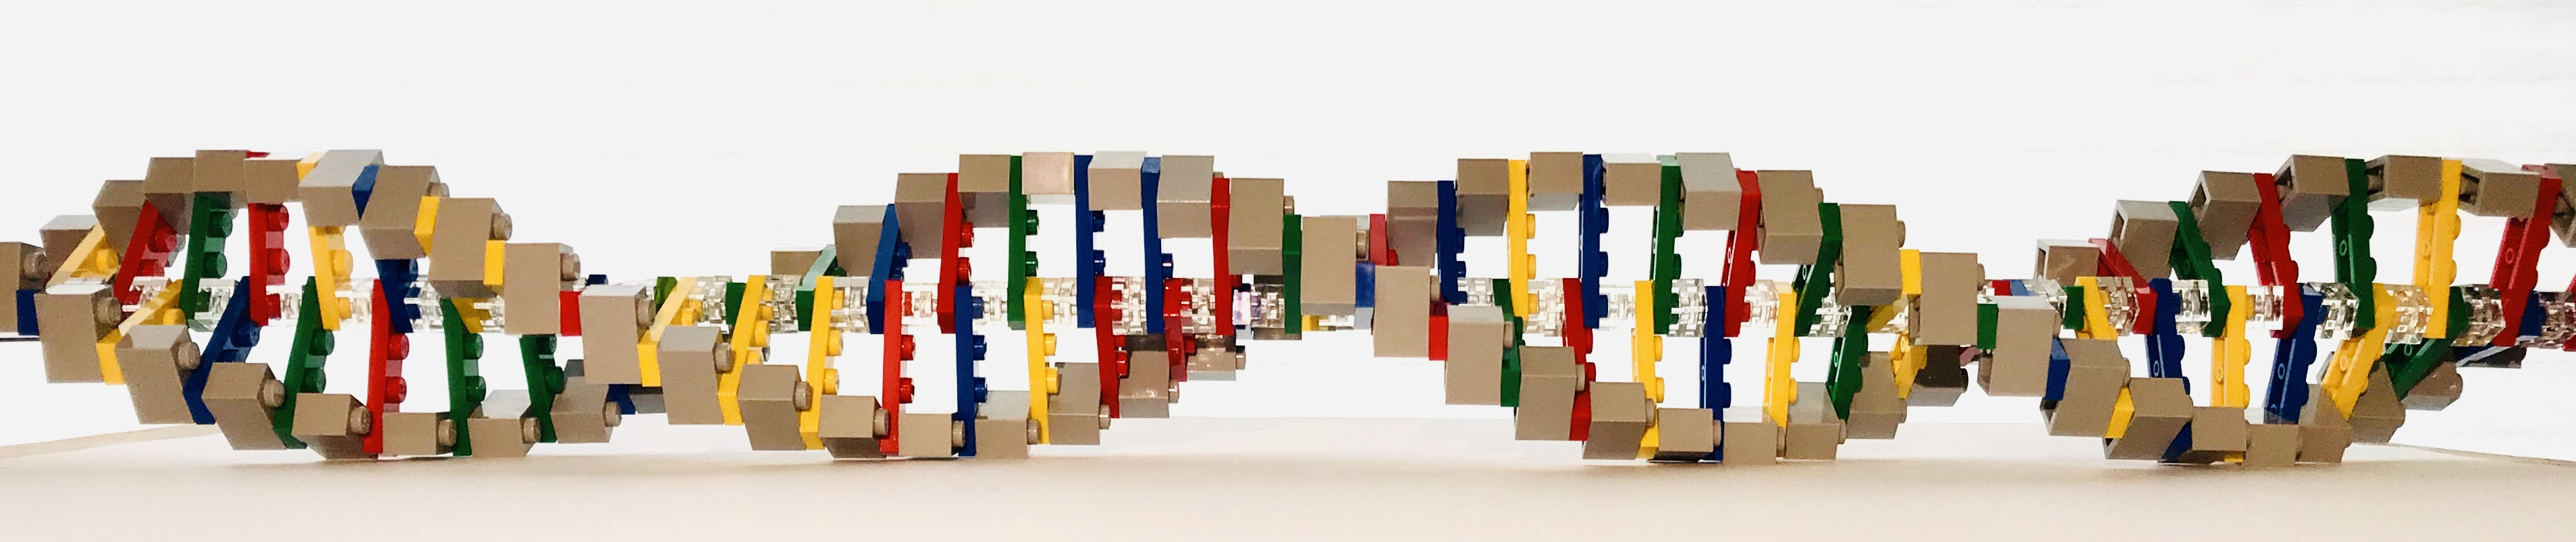
\includegraphics[width=1\linewidth]{static/images/DNA} \end{center}

First, I would like to acknowledge the Genome Education Partnership (\href{http://gep.wustl.edu/curriculum/introducing_genes}{GEP}) for inspiration. They created a resource for learning about Eukaryotic gene structure using the UCSC Genome Browser (Laakso et al.~2017). Their focus is on the \emph{Drosophila} genome. My focus is on the \emph{human} genome. My hope is that the skills learned within these pages and the saved sessions I have created (and will continue to curate) can be used as a springboard for continued exploration of the human genome.

© 2019, Maria Gallegos. All rights reserved.

\hypertarget{overview}{%
\section*{Overview}\label{overview}}
\addcontentsline{toc}{section}{Overview}

Throughout the semester, you will use a web-based visualization tool called a Genome Browser to explore gene structure and function in humans. We will focus on the human gene, BBS1. BBS1 has been implicated in Bardet Biedl Syndrome, a pleiotropic\footnote{pleiotropy is a condition in which a single gene influences more than one trait (Snustad).} disease with a variety of symptoms including blindness, obesity, polydactyly, cognitive impairment, renal abnormalities, infertility and anosmia. In addition to learning how to navigate through the genome browser, you will also learn how to

\begin{enumerate}
\def\labelenumi{\arabic{enumi}.}
\tightlist
\item
  Use the Genome Browser to examine gene structure within a genome (Chapter 3)
\item
  Use the Genome Browser to analyze RNA evidence pinpointing the location of genes (Chapters 4 and 5).
\item
  Identify DNA and RNA sequence motifs critical for gene expression (Chapters 6 and 7).
\item
  Identify and assess pathogenic and benign mutations (Chapter 8).
\item
  Analyze sequence conservation between human genes and genes in simpler model organisms (Chapter 9).
\end{enumerate}

\hypertarget{how-to-use-this-manual-efficiently}{%
\section*{How to use this manual efficiently}\label{how-to-use-this-manual-efficiently}}
\addcontentsline{toc}{section}{How to use this manual efficiently}

This manual can be viewed on a computer, tablet or phone. That said, navigating through the UCSC genome browser is much easier on a laptop or desktop computer. Moreover, the instructions I provide assume you are using one of the two. When on a computer, the table of contents (side bar) can be toggled in and out by typing ``s''. And the arrow keys can be used to move to later or earlier chapters.

All figures can be enlarged by clicking on an image of interest. To reduce the image back to its original size and continue reading, click on the enlarged image again.

Throughout this tutorial, you will come across footnotes. When you click on the link to a footnote, you will be taken to the end of the chapter to read it. To continue reading, click the return arrow at the end of the footnote. It is a good idea to read the footnotes and figure legends! These are provided to clear up confusion. They might also provide clues to answering ``Test Your Understanding'' questions (see below).

``Test your understanding'' (TYU) and ``For Discussion'' headings are all clickable and take you to the corresponding ``Google quiz'' in a new tab. That said, \textbf{you need to be logged into your horizon email account in order to access them}. Also, you will NOT receive response receipts. You can answer each quiz multiple times and after you submit you can check your accuracy. You will NOT receive an email confirmation with your answers to the questions. So long as you don't snap your computer shut before the form has been submitted, I will receive it. Your goal is to eventually figure out how to get the right answer. TYU questions are designed to see if you understand how to navigate through the genome AND if you understand what you are seeing. It is best to get the answers correct before moving on. I will be available during activity section to answer any questions you might have.

Finally, it is best to read this manual with a pen and notebook in hand for taking notes AND for recording your answers to TYU and ``For Discussion'' questions. If on the off chance your Google Quiz submission fails, you have your answers written down for an easy re-submission.

Also, if you spot any errors or typos. Please let me know via Slack. Thanks!

\hypertarget{before-you-get-started}{%
\section*{Before you get started}\label{before-you-get-started}}
\addcontentsline{toc}{section}{Before you get started}

Before you get started, you should create an account at the UCSC Genome Browser web site. Creating an account at the UCSC Genome Browser site is useful for a variety of reasons. For example, having an account will enable you to save your favorite settings into a named session, and then return to the named session later regardless of which computer you use. You can also share named sessions with other users (something I will do for you throughout the semester).

To create an account, go to the \href{https://genome.ucsc.edu/}{UCSC Genome Browser}. In the toolbar at the top of the page hover over ``My Data'' then choose ``My Sessions'' from the pulldown menu. At the top of the page click ``Create an Account''. Complete the form then click ``Sign Up''. You are done!

\hypertarget{an-introduction-to-genes-and-genomes}{%
\chapter{An Introduction to Genes and Genomes}\label{an-introduction-to-genes-and-genomes}}

\hypertarget{what-is-a-gene}{%
\section{What is a gene?}\label{what-is-a-gene}}

A \textbf{gene} is a segment of DNA that directs the production of a functional product. A significant number of eukaroytic genes are protein coding. Each protein-coding gene is used as a template to create an \textbf{RNA transcript} through a process called \textbf{transcription}. The RNA transcript is then processed into a messenger RNA (mRNA). The most notable change that occurs during RNA processing is that intron sequences are removed from the RNA transcript leaving behind exons. This processed mRNA is then exported from the nucleus and used as a template to make a protein in a process called \textbf{translation} (Figure \ref{fig:geneexpression}). Proteins do most of the work necessary to maintain cell structure, function and behavior.

\begin{figure}

{\centering 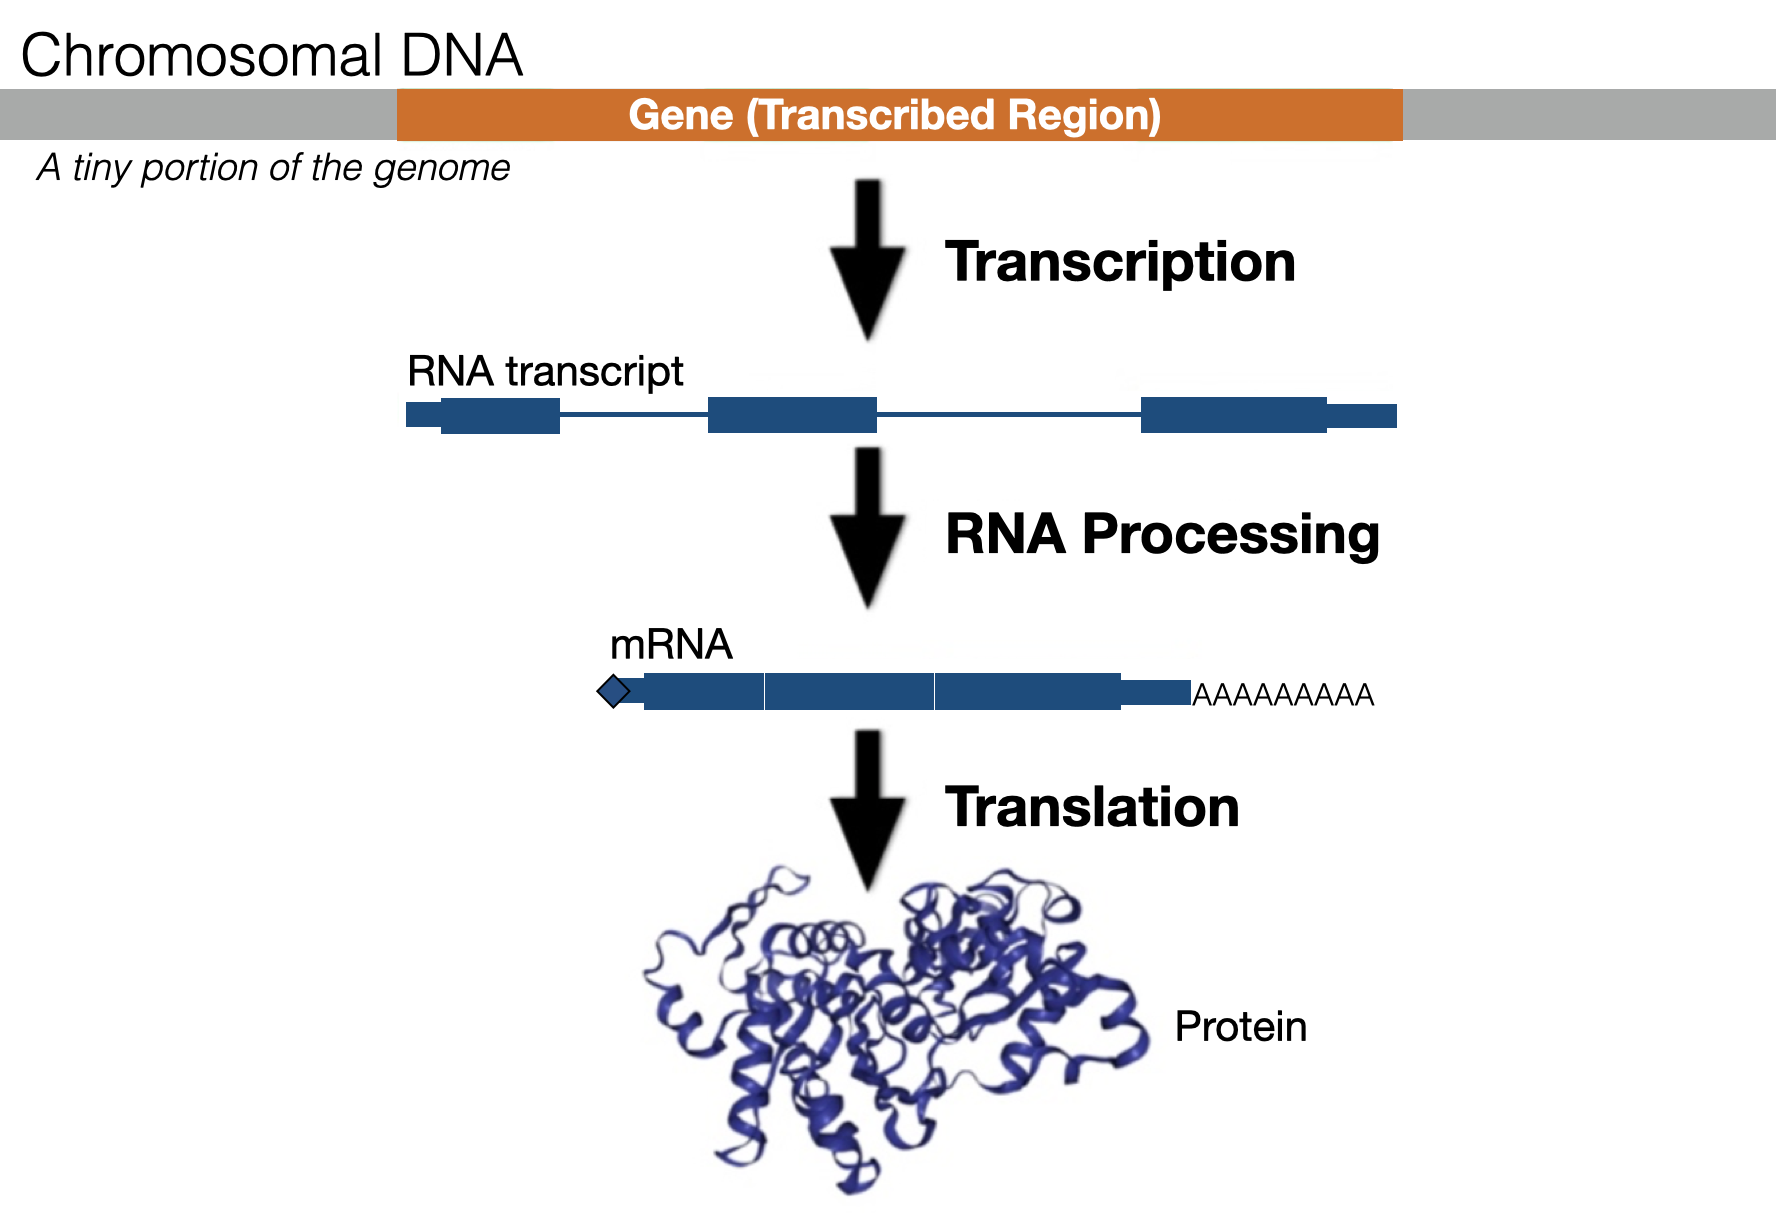
\includegraphics[width=0.75\linewidth]{static/images/gene}

}

\caption{An overview of Gene Expression. A small segment of DNA (light grey) containing a single gene (orange) is shown. The RNA transcript is highlighted in green (exons) and dark gray (introns).}\label{fig:geneexpression}
\end{figure}

Importantly, the size of a gene is usually defined by where transcription begins and ends. In fact, the site of \textbf{transcription initiation} and \textbf{transcription termination} define both the gene size (in the genome) and the RNA transcript size (but not the mRNA size which is typically shorter).

\hypertarget{what-is-a-genome}{%
\section{What is a genome?}\label{what-is-a-genome}}

These 24,000 protein coding genes are distributed linearly along chromosomes\footnote{a \href{https://www.nature.com/scitable/definition/chromosome-chromosomes-eukaryotic-chromosome-eucariotic-chromosome-procariotic-6/}{chromosome} is a single, long molecule of DNA} (Figure \ref{fig:genomesegment}).

\begin{figure}

{\centering 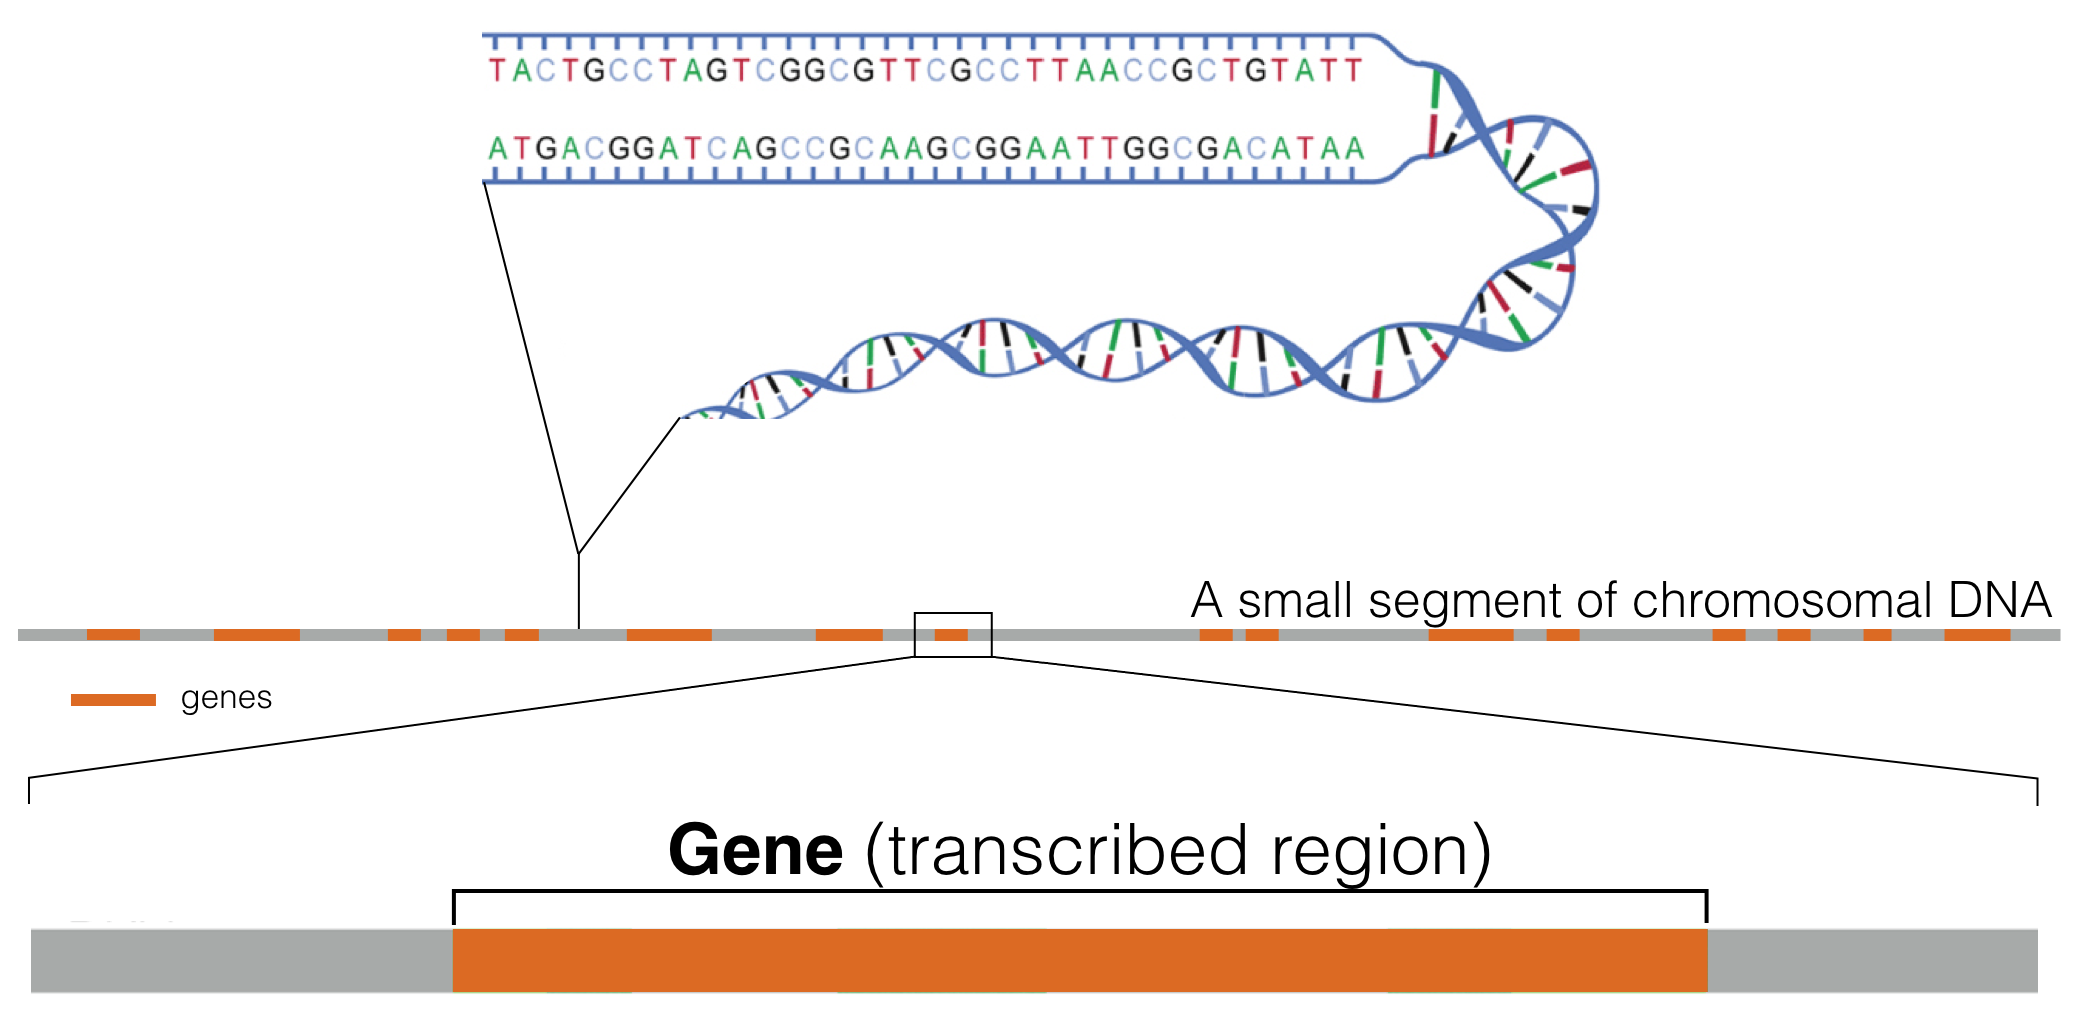
\includegraphics[width=1\linewidth]{static/images/partofgenome}

}

\caption{This schematic represents a hypothetical segment of a chromosome with orange rectangles representing genes distributed linearly along the DNA segment shown.}\label{fig:genomesegment}
\end{figure}

One complete set of genes/chromosomes inherited from a single parent makes up what we call the genome (sometimes called the ``haploid genome'')\footnote{While ``haploid genome'' is more precise, ``haploid'' is often omitted and simply assumed}. The haploid genome consists of 23 chromosomes in XX females and 24 in XY males. Each chromosome varies in length. For example, chromosome one is the longest. It is a double helix of 248,956,422 base pairs (bp) and is 82.7 mm in length \footnote{To calculate the length of each chromosome you multiple the length of the chromosome in base pairs (bp) by the length (in mm) of each bp (0.000000332).} (Figure \ref{fig:genome}).

\begin{figure}

{\centering 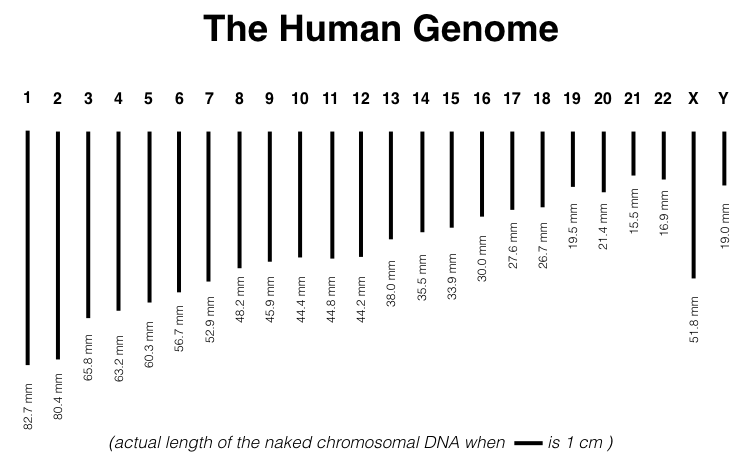
\includegraphics[width=0.9\linewidth]{static/images/humangenome}

}

\caption{Actual length of the human genome when scale bar equals one centimeter.}\label{fig:genome}
\end{figure}

In diploid organisms like humans, somatic cells (i.e.~skin, neurons etc) harbor \emph{two} complete sets of chromosomes. Thus, in total, there is just over two meters of DNA crammed into each somatic nucleus! The diameter of a mammalian nucleus is 6 microns or 0.006 of a millimeter (on average). How does all this DNA fit? First, the \emph{diameter} of a DNA double helix is tiny (only 2 angstroms) but also each chromosome is carefully packaged by proteins in a systematic and sterotypical manner (Figure \ref{fig:chromatin}).

\begin{figure}

{\centering 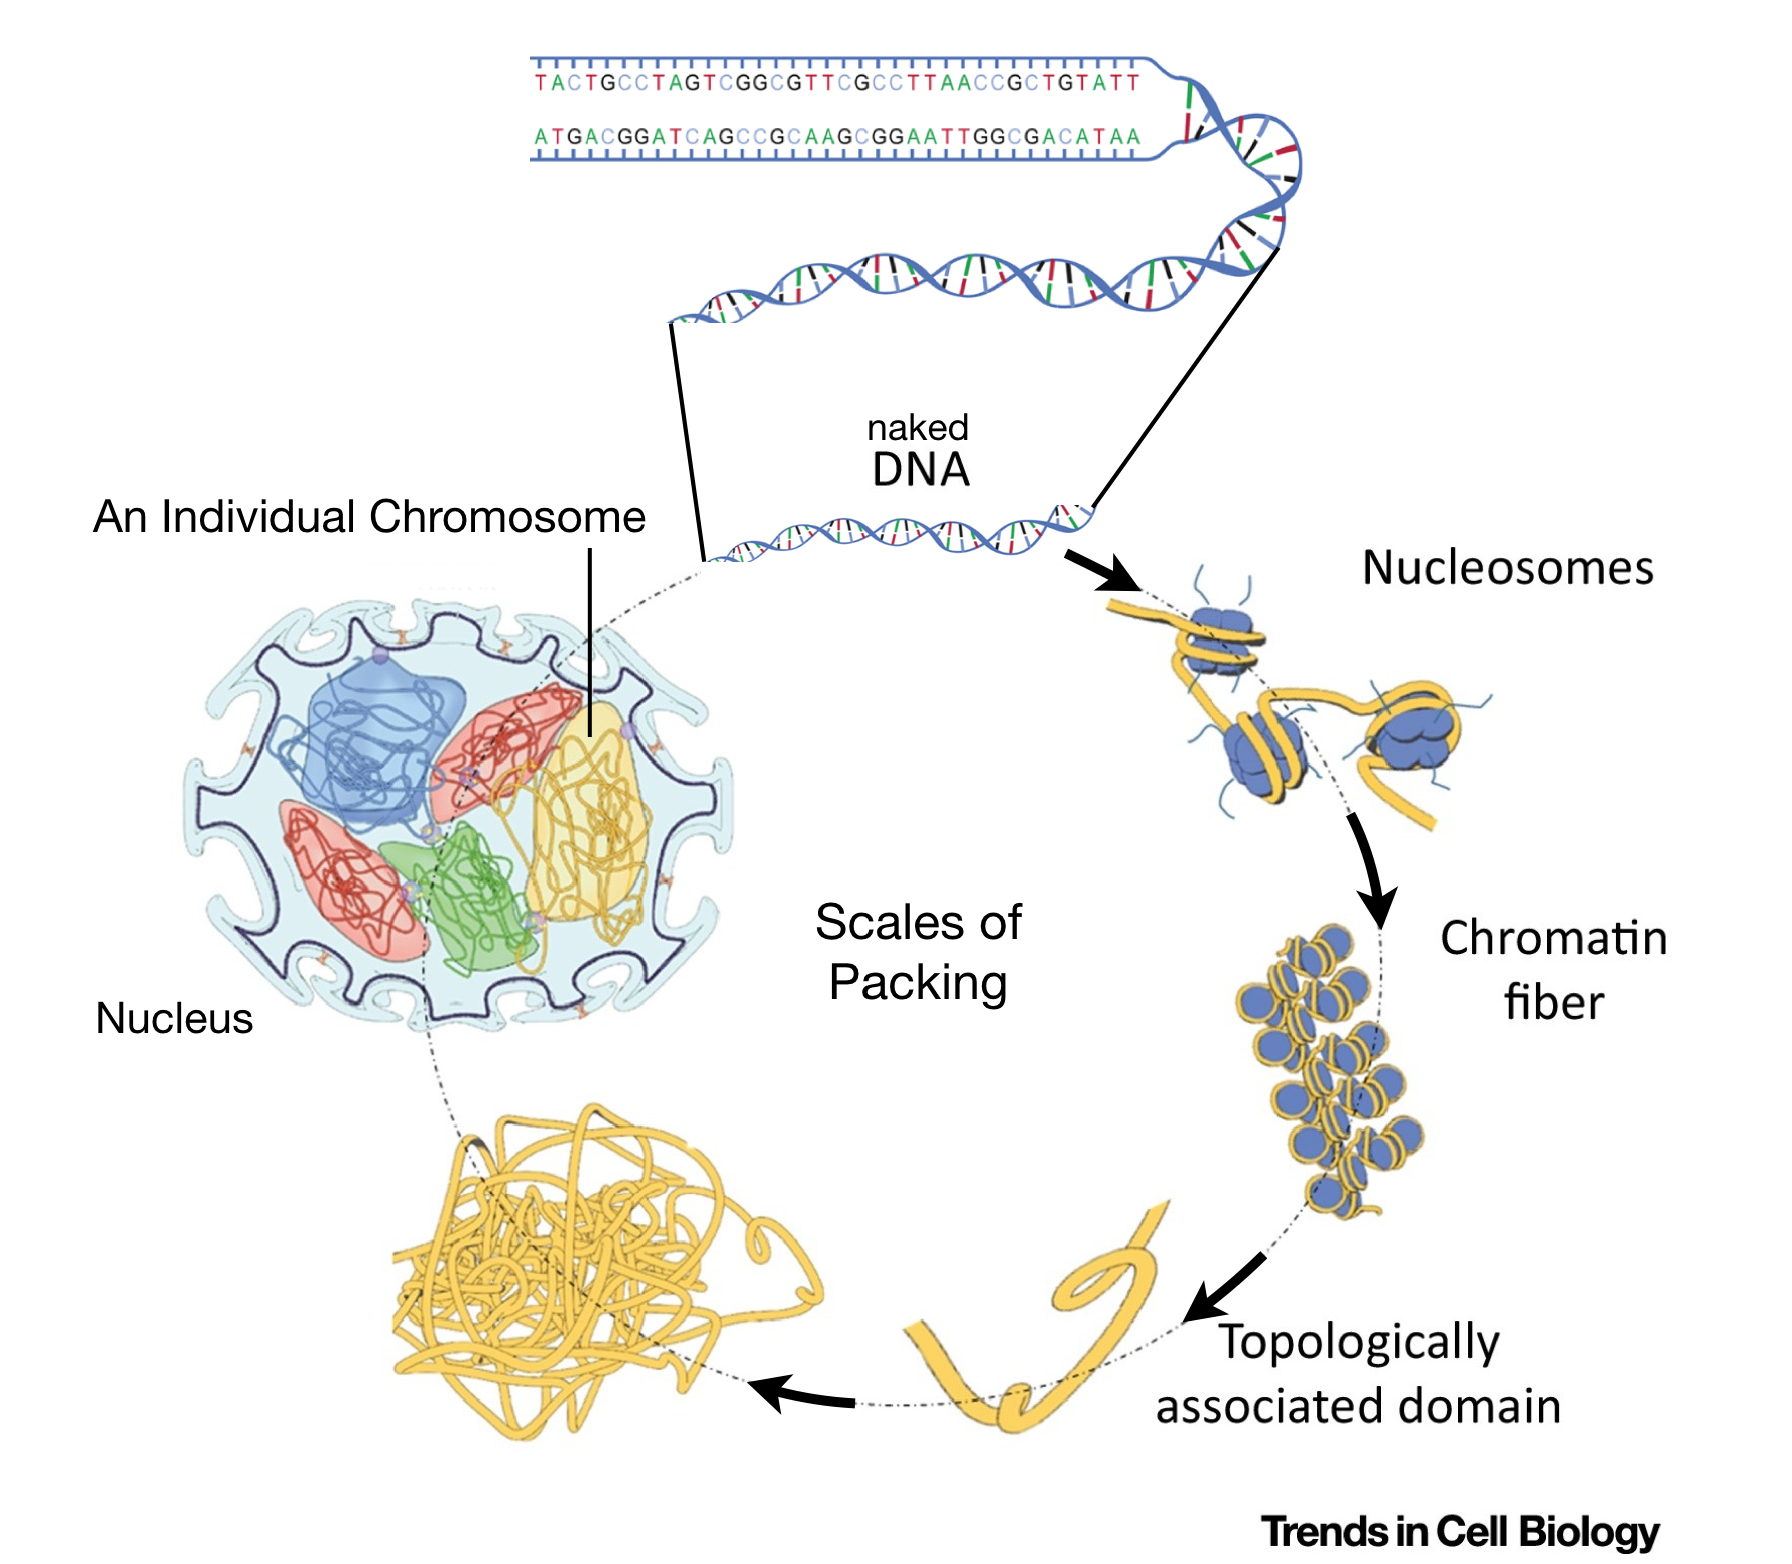
\includegraphics[width=0.9\linewidth]{static/images/interphasechromatin}

}

\caption{This image is modified from Uhler and Shivashankar, 2017. It shows the various levels of chromosome packing found in nuclei during interphase of the cell cycle. The first level of packing requires an octamer of histone proteins that assemble into a ball-like structure called a *nucleosome*. Naked DNA wraps around these octamers forming 'beads on a string'. Additional levels of packing into chromatin fibers and topological associated domains requires additional proteins. Individual chromosomes (23 pairs in humans) are then carefully orgnanized within the cell nucleus in a cell type-dependent manner.}\label{fig:chromatin}
\end{figure}

\hypertarget{test-your-understanding}{%
\subsection{\texorpdfstring{\href{https://docs.google.com/forms/d/e/1FAIpQLSe8eECUs8Zwm1bFPFWeCK5DKgM4zM0zaRyZNIYWvjbwk1XFAA/viewform?usp=sf_link}{Test Your Understanding}}{Test Your Understanding}}\label{test-your-understanding}}

\begin{itemize}
\tightlist
\item
  \emph{Which happens first (RNA processing, transcription or translation - written in alphabetical order)?}
\item
  \emph{Where does RNA processing occur?}
\item
  \emph{Where does transcription occur?}
\item
  \emph{Where does translation occur?}
\item
  \emph{TRUE or FALSE. If I told you the size of a mature mRNA transcript you would know the size of the gene in the genome?}
\item
  \emph{Chromosome 1 is the longest chromosome at 82.7 mm. How long is it in inches (round to the first decimal place)?}
\item
  \emph{The longest chromosome in C. elegans is chromosome V. It is 20,924,180 bp. How long is it in mm (round to the nearest whole mm)?}
\item
  \emph{In humans, there is just over two meters of DNA crammed into each somatic nucleus. What can you find around your house that is about two meters in length?}
\item
  \emph{Fill in the blank. The first level of chromosomal packing requires an octamer of histone proteins that assemble into a ball-like structure called a \_\_\_\_\_\_\_}
\item
  \emph{TRUE or FALSE. Each chromosome occupies its own 3-dimensional space within the nucleus. Chromosomes are NOT mixed together like a bowl of spaghetti.}
\end{itemize}

© 2019, Maria Gallegos. All rights reserved.

\hypertarget{an-introduction-to-the-ucsc-genome-browser}{%
\chapter{An Introduction to the UCSC Genome Browser}\label{an-introduction-to-the-ucsc-genome-browser}}

The UCSC genome browser harbors the sequence of a reference genome\footnote{``A reference genome (also known as a reference assembly) is a digital nucleic acid sequence database, assembled by scientists as a representative example of the set of genes in one idealized individual organism of a species. As they are assembled from the sequencing of DNA from a number of individual donors, reference genomes do not accurately represent the set of genes of any single individual organism. Instead a reference provides a haploid mosaic of different DNA sequences from each donor''. - from Wikipedia} (24 linear chromosomes and the mitochondrial genome). In this chapter, I explain how the UCSC Genome Browser is organized, how to open and configure evidence tracks and how to move through the Genome Browser. That said, we will mainly focus our Browser window on a single gene, BBS1.

\hypertarget{how-to-configure-the-genome-browser}{%
\section{How to Configure the Genome Browser}\label{how-to-configure-the-genome-browser}}

\begin{figure}

{\centering 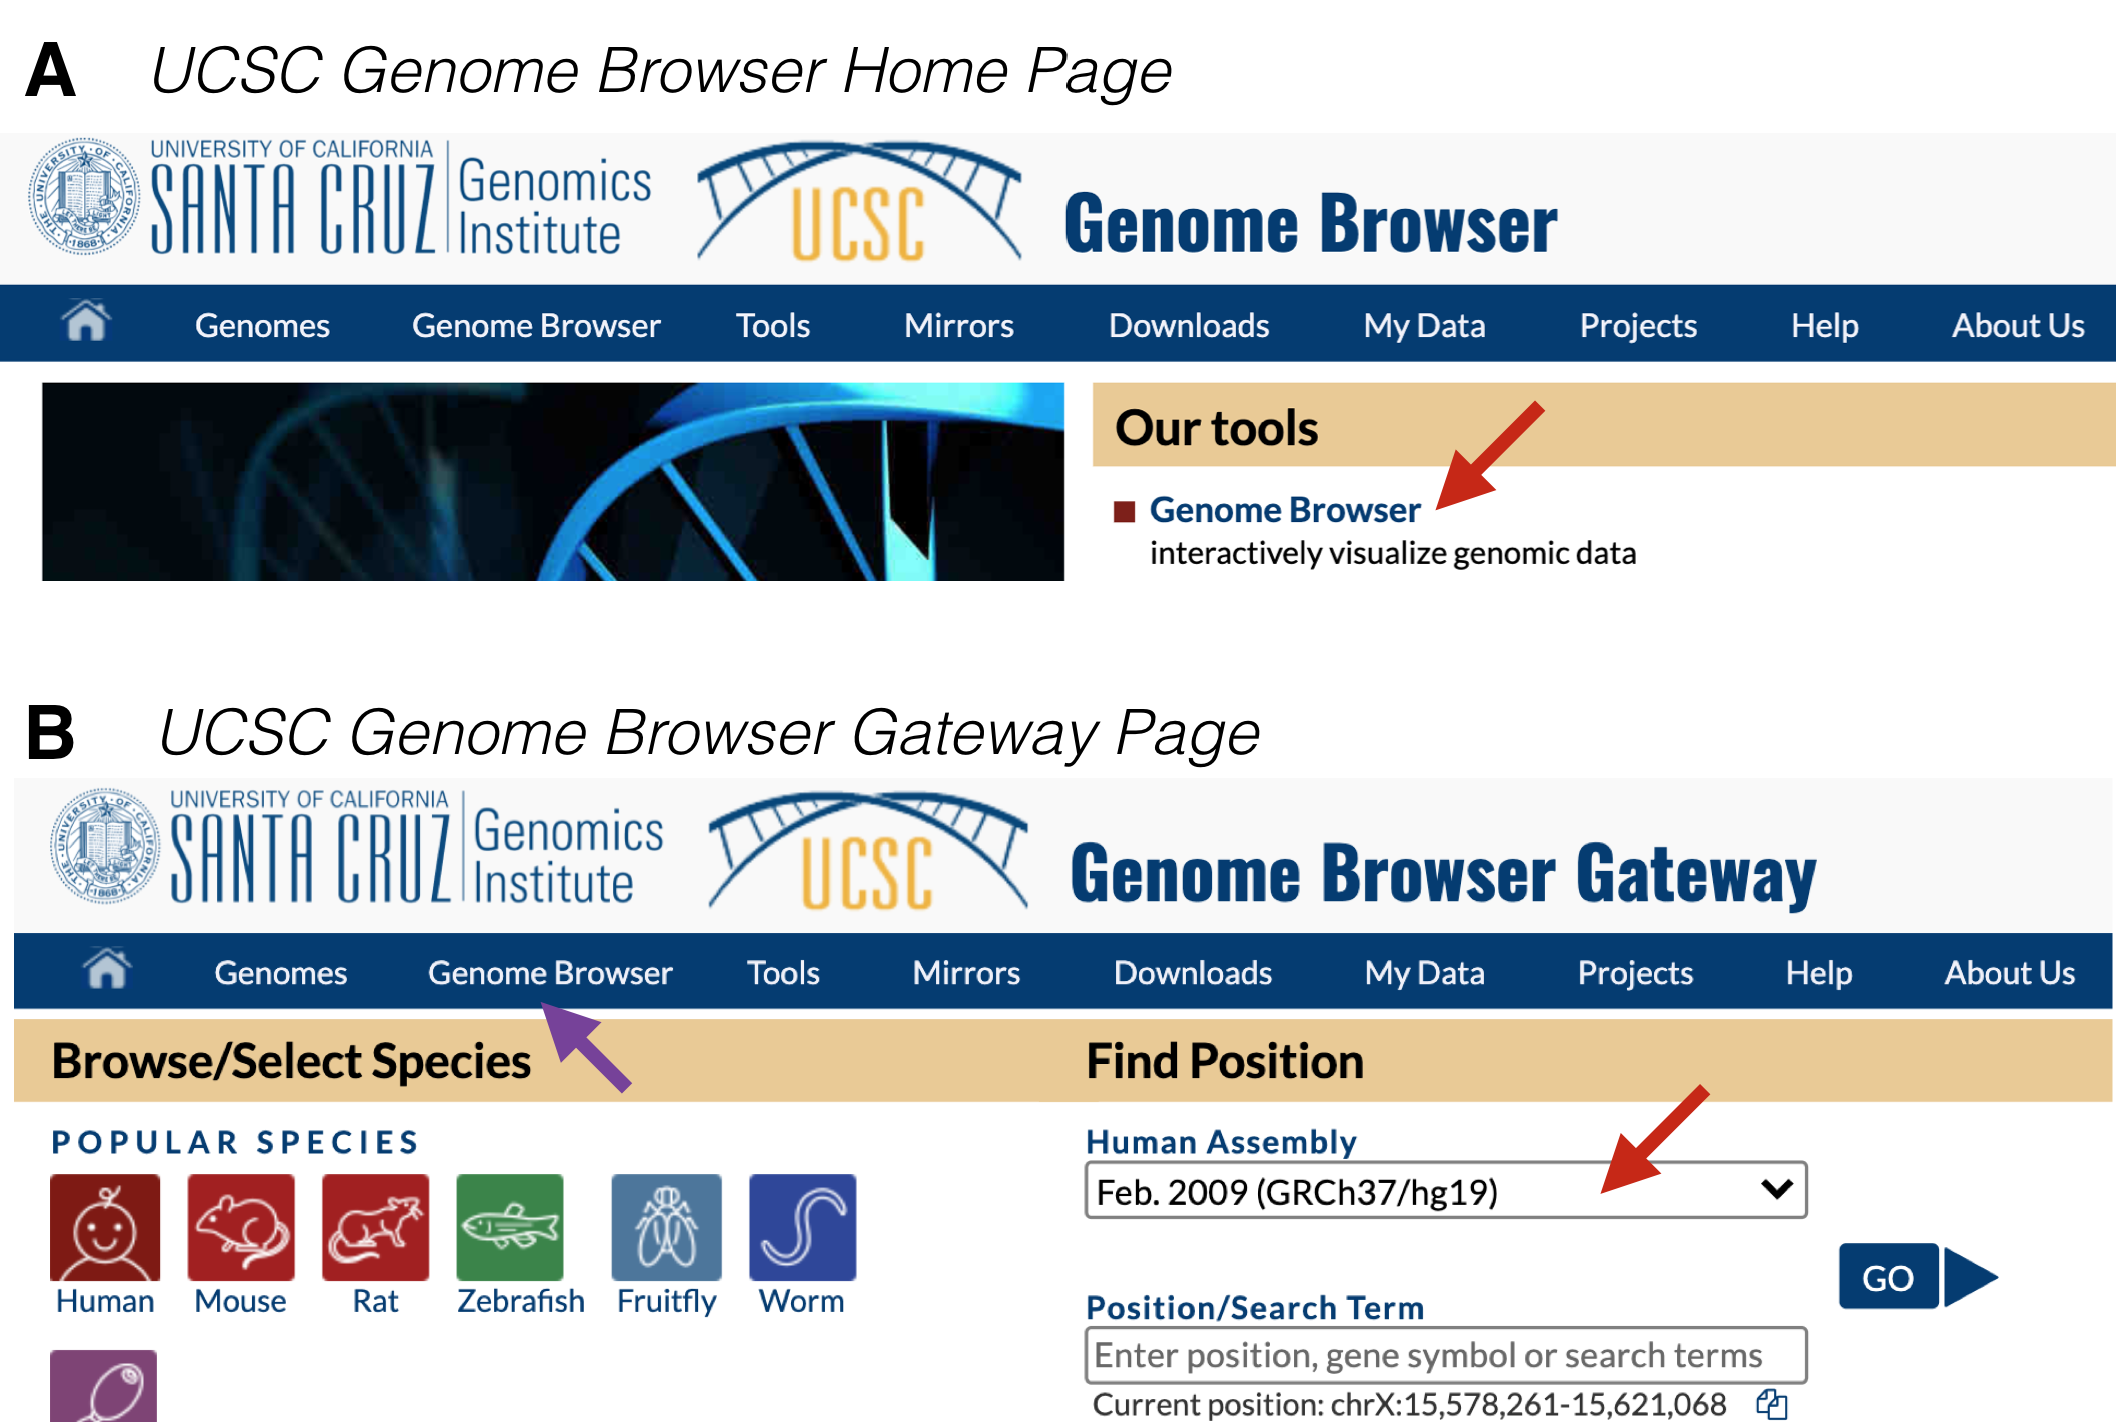
\includegraphics[width=0.5\linewidth]{static/images/browsergateway}

}

\caption{A) This is the UCSC Genome Browser Homepage. Click on *Genome Browser* (red arrow) to get to the Browser Gateway Page. B) This is the Browser Gateway Page. Choose the *Feb. 2009* Human assembly (red arrow) then click *Go*.}\label{fig:gateway}
\end{figure}

To begin from scratch, go to the \href{https://genome.ucsc.edu/}{UCSC Genome Browser}. At the home page, click on ``Genome Browser'' under ``Our Tools'' (Figure \ref{fig:gateway} A). Within the Genome Browser Gateway page, hover your mouse over ``Genome Browser'' in the tool bar (Figure \ref{fig:gateway} B, purple arrow) and click on ``Reset All User Settings''. Then click on the pull down menu under Human Assembly\footnote{A Genome Assembly is a whole genome sequence produced after chromosomes have been fragmented, sequenced, and the resulting sequences have been put back together (assembled). Each time the genome is sequenced, errors are corrected then uploaded as a new genome assembly. The Feb.~2009 is still the most popular assembly to date with the most useful evidence tracks.} and choose ``Feb.~2009 (GRCh37/hg19)'' (Figure \ref{fig:gateway} B, red arrow). Now click ``Go'' to be taken to the Human Genome Browser window.

Since you did not search for a specific gene, you have been taken to a default position within the genome, specifically, a small region on the \textbf{short arm} of the X chromosome where a gene called ACE2 resides (Figure \ref{fig:ACE2} A and B). Why here? This paragraph was written in 2020 when ACE2 became \emph{infamous}. Google ``ACE2'' and ``coronavirus'' to see why!

\begin{figure}

{\centering 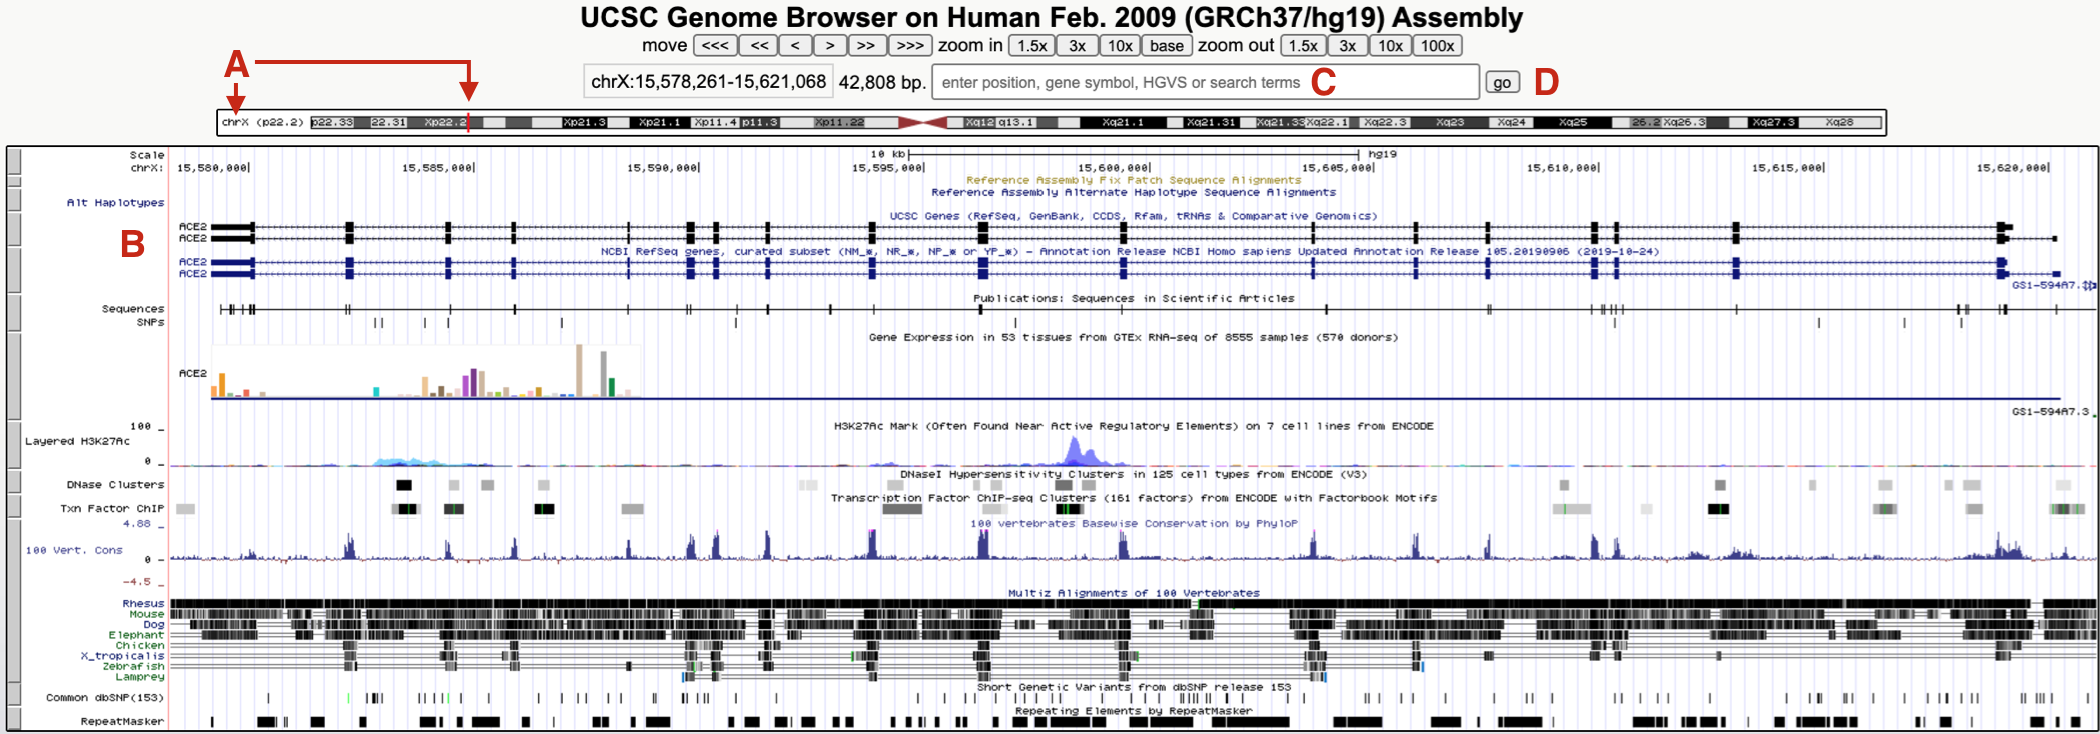
\includegraphics[width=1\linewidth]{static/images/ACE2gene}

}

\caption{The UCSC Genome Browser window focused on a small region of the X chromosome (A) on a gene called ACE2 (B). To hop to BBS1, use the search window (C) then click *Go* (D). See text for important details.}\label{fig:ACE2}
\end{figure}

To hop to where BBS1 resides, type BBS1 into the search window (Figure \ref{fig:ACE2} C). \textbf{As you type, a popup menu will appear with a short list of related genes}. Choose BBS1 then click ``GO'' (Figure \ref{fig:ACE2} D). If you \emph{do not} choose a gene from this list, you will be transported to a new page with a long list of related genes grouped according to sequence database (there are many). It might be easiest to go back and try again. Alternatively, scroll down until you find the ``NCBI RefSeq'' database\footnote{The ``NCBI RefSeq'' database is the one we will be using.} then click on the link for BBS1.

Your browser window should now jump to chromosome 11 (Figure \ref{fig:BBS1} A). The default genome browser window will now display a variety of so-called ``evidence tracks''. These are graphical representations of genome features or experimental data related to the region displayed. Nearly all evidence tracks include a centrally located title heading (Figure \ref{fig:BBS1} B) and all include a gray rectangle positioned on the left (Figure \ref{fig:BBS1} C). Three evidence tracks are highlighted in total. The one at the top is the \textbf{Base Position} track (Figure \ref{fig:BBS1} D). This is the only evidence track that \emph{does not have a track title}. This track displays the genome sequence itself. That said, you will only be able to see individual nucleotides when you zoom in close enough. Two \textbf{Gene Prediction} tracks are also highlighted. One is the ``UCSC Genes'' track (Figure \ref{fig:BBS1} E). Another is the ``NCBI Refseq genes'' track (Figure \ref{fig:BBS1} C). Notice the gene name is displayed on the left side of each schematic.

\begin{figure}

{\centering 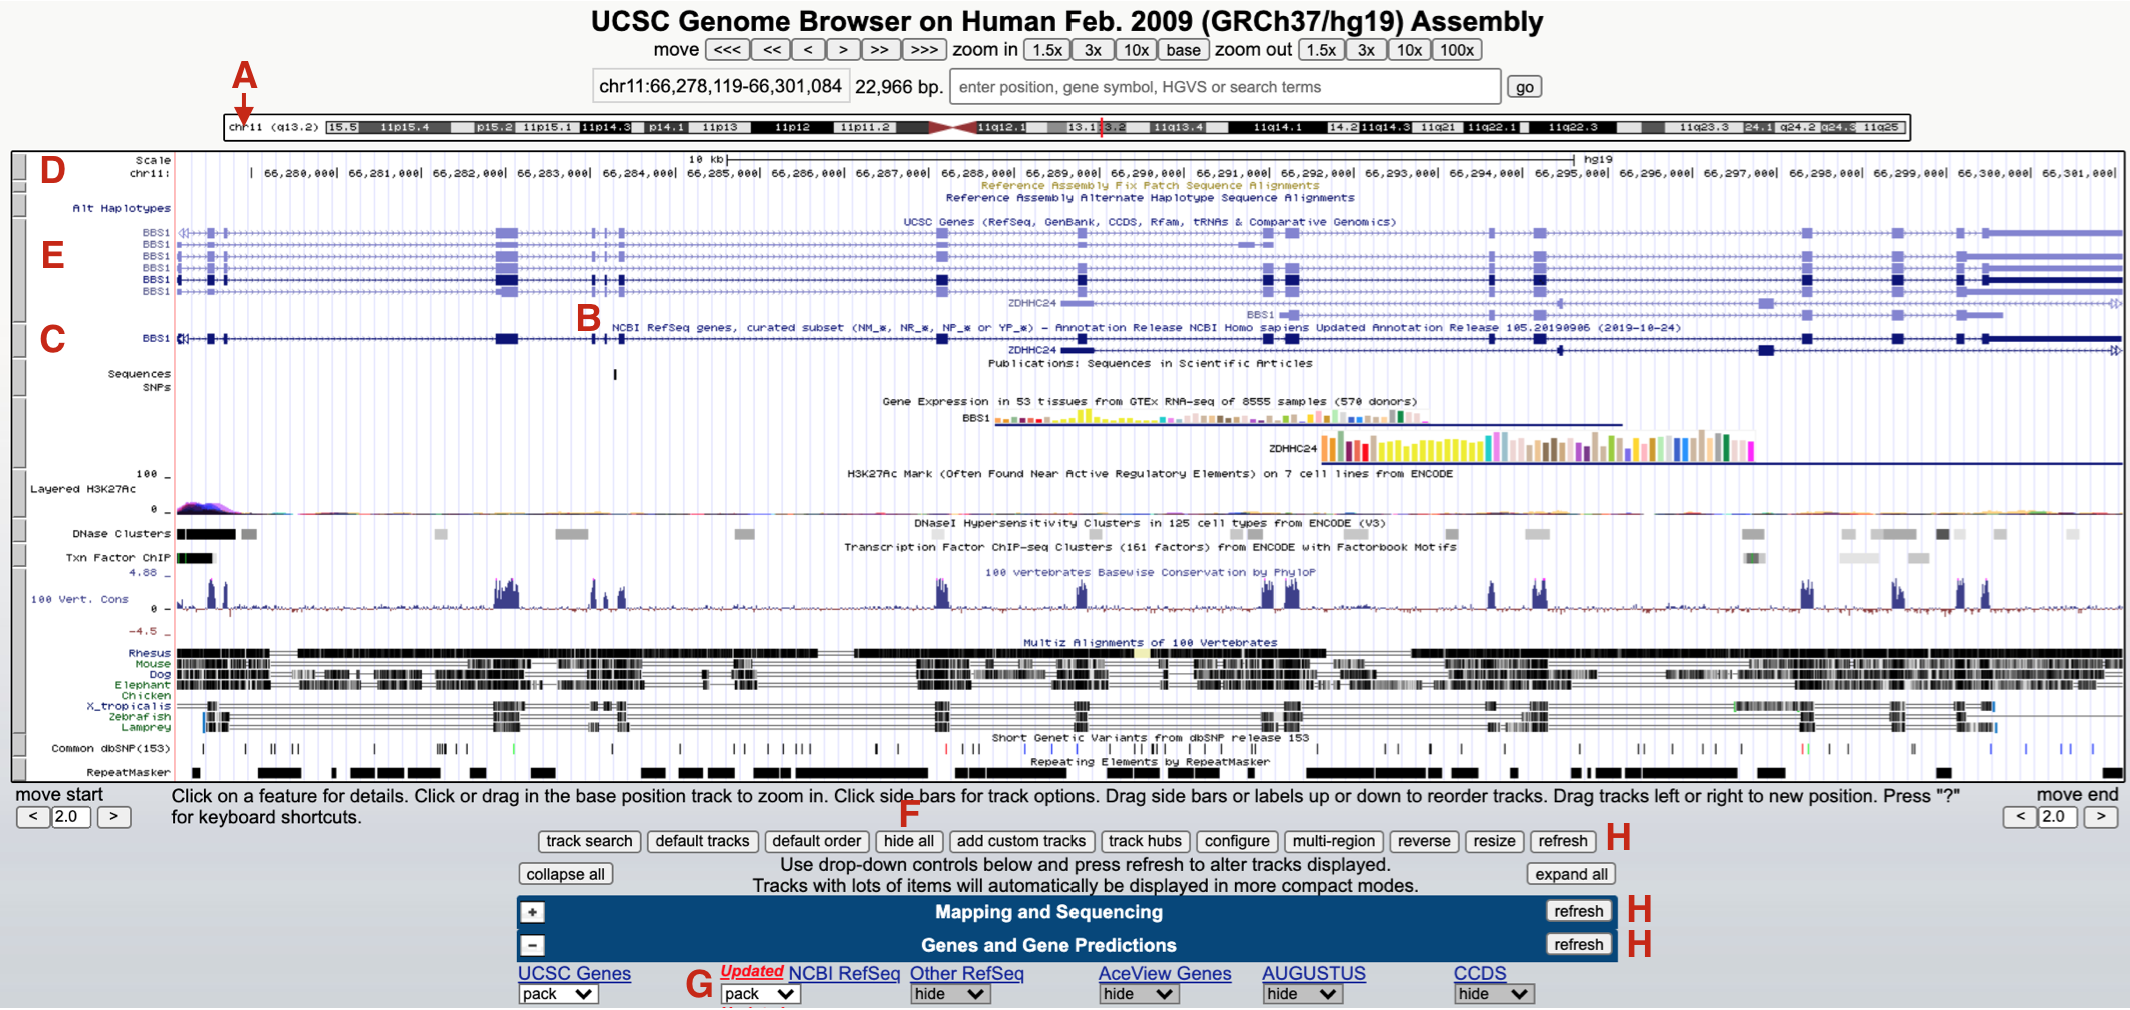
\includegraphics[width=1\linewidth]{static/images/BBS1gene}

}

\caption{The browser window now focused on a small region of chromosome 11 (A) where BBS1 resides (C and E). Each evidence track includes a track title (B) and is demarcated by a gray rectangle (D, E and C). To hide all tracks click *hide all* (F) and click *refresh* (H). To open the NCBI Refseq track change the pulldown menu from *hide* to *pack* (G).}\label{fig:BBS1}
\end{figure}

Each gray rectangle corresponding to an evidence track is clickable. Clicking on a gray rectangle will take you to a track settings page for that particular evidence track. Try it. Then click the back button to get back. Right clicking on a gray rectangle on the other hand will open up a small window for \emph{quick} formatting. For example, you can hide any evidence track that you don't need in this way. To hide all evidence tracks at once, scroll down to below the browser window and click ``hide all'' (Figure \ref{fig:BBS1} F). Everything but the Base Position track will disappear. Now scroll down to view the most commonly used evidence tracks below the browser window to confirm. All but the ``Base Position'' track found within the ``Mapping and Sequencing'' section should be set to hide. \textbf{Now change the ``NCBI Refseq'' evidence track (found within the ``Genes and Gene Predictions'' section) to ``pack''} (Figure \ref{fig:BBS1} G) \textbf{and click ``refresh''} (Figure \ref{fig:BBS1} H). You should now see only two gray rectangles on the left. The base position track on top and the ``NCBI refseq genes'' Gene Prediction track is below (Figure \ref{fig:BBS1simple}).

\begin{figure}

{\centering 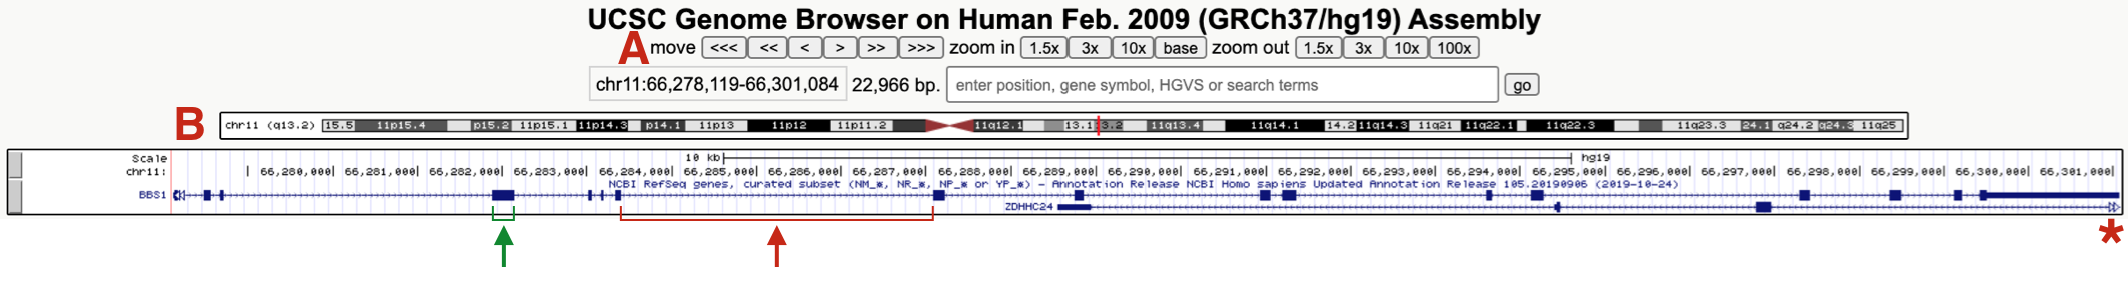
\includegraphics[width=1\linewidth]{static/images/BBS1genesimple}

}

\caption{This is what the *BBS1 Gene Structure* named session should look like. One example of an exon and intron are highlighted. The asterix points on the right highlights the open triangles extending from ZDHHC24 indicating that this gene extends further to the right. (A) highlights the navigational toolbar and (B) highights the schematic of the chromosome where BBS1 resides. One exon (green bracket) and one intron (red bracket) are also shown.}\label{fig:BBS1simple}
\end{figure}

Again, the ``NCBI Refseq genes'' evidence track includes a graphical representation of the BBS1 gene\footnote{Gene: Genome browsers provide a precise position for each gene, in reality, we don't really know where a gene truly begins or ends (there is sequence both upstream and downstream of the RNA transcript that is important for regulating gene expression). That said, we can experimentally determine the transcribed region of a gene. Thus, it makes most sense to equate the transcribed region of a gene to the gene itself even though we know more sequence is required for the gene to be transcribed properly.}. This gene schematic displays the position of BBS1 exons and introns (see red and green brackets in Figure \ref{fig:BBS1simple}). You may also notice that a second gene (ZDHHC24) partly overlaps BBS1. The open arrowheads at the far right of the graphical representation for ZDHHC24 (red asterisk, Figure \ref{fig:BBS1simple}) indicates that this gene extends farther to the right.

\hypertarget{creating-a-named-session}{%
\section{Creating a Named Session}\label{creating-a-named-session}}

Compare what you configured to my named session, \href{https://genome.ucsc.edu/s/megallegos/Biol\%20310\%20Module\%201}{BBS1 gene structure}. If they are identical, congratulations. If not, try again but don't stress too much. You can always use my link to get to a correctly formatted page. You are now ready to create your own named session based on the browser window you created (or mine). First, make sure your browser window looks the way you want it to. Next, make sure you are logged into your account. Hover your mouse over ``My Data'' then click on ``My Sessions''. Scroll down to the section entitled, ``Save Settings''. Within the window under ``Save current settings as named session'', input a reasonable name for this session (i.e.~``Gene and Base Prediction Tracks only''). Then hit submit. Now anytime you want to sit down at a computer (anywhere, any computer) to view BBS1 with only the base position and gene prediction tracks open, you simply need to log into your UCSC Genome Browser account, go into ``My Sessions'' and click on your named session. You won't need to rely on this manual for links. \textbf{You can also use this named session as a springboard to view any other gene by using the search window.}

\hypertarget{navigating-around-in-the-genome-browser}{%
\section{Navigating Around in the Genome Browser}\label{navigating-around-in-the-genome-browser}}

Above the browser window you will find the navigational toolbar (Figure \ref{fig:BBS1simple} A). You can use the buttons within the navigational toolbar to scroll left \textless\textless\textless{} or right \textgreater\textgreater\textgreater{} or zoom in or out. Directly below the navigational toolbar is a schematic representation of chromosome 11 where BBS1 is located (Figure \ref{fig:BBS1simple} B). The red vertical line (not easy to spot) indicates where the browser window is focused within this chromosome.

Practice navigating through the genome browser. Zoom in. Zoom out. Scroll left. Scroll right. Click on a random position within the chromosome schematic. Hover your mouse over various elements in the browser window to read pop-up messages. Click on any feature for more details. Click the gray rectangles on the left side to access track settings. Change track settings to see the impact. If/when you get hopelessly lost in the genome or the formatting changes in an undesirable way, use your named settings link to get back.

The most important navigational trick to learn is how to \textbf{``drag select or click to zoom''} from within the base position track. This trick will allow you to zoom in to a specific location within the browser window, a navigational trick we will use repeatedly. Master it now. Hover your mouse \emph{within} the base position track until a tiny ``drag select or click to zoom'' popup message displays. Now you are in the right place to ``click'' then ``drag'' (with your finger on the trackpad) to perform the ``Drag-and-Select'' trick. When you do it correctly, you will create a box around the portion of the gene you want to zoom into (red arrow, Figure \ref{fig:select}) AND you will open a ``Drag-and-Select'' window. Can't get ``click and drag'' to work? Hover your mouse \emph{within} the base position track until a tiny ``drag select or click to zoom'' popup message displays. Now you are in the right place to ``right click'' or ``click'' then drag to perform the ``Drag-and-Select'' trick.

\begin{figure}

{\centering 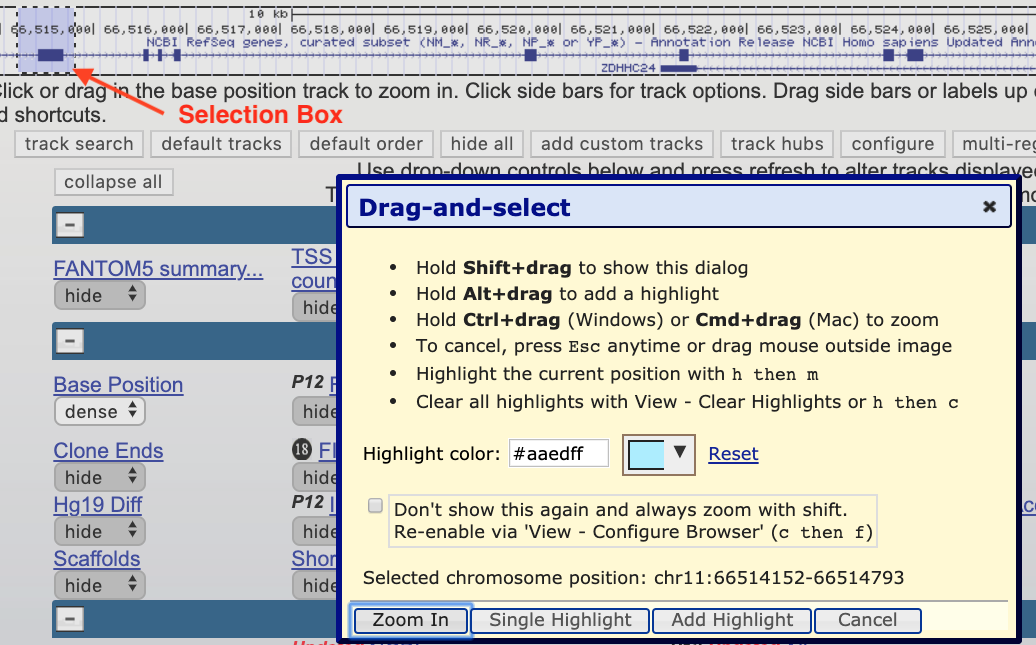
\includegraphics[width=1\linewidth]{static/images/dragnselect}

}

\caption{The drag select or click to zoom tool is very useful.}\label{fig:select}
\end{figure}

If you zoom in close enough you will begin to see the nucleotide sequence of the human genome. The exon intron boundaries are clearly aligned to this geneome sequence. For example, in Figure \ref{fig:zoomtosequence}, the exon shown begins with the sequence: G-A-C-C.

\begin{figure}

{\centering 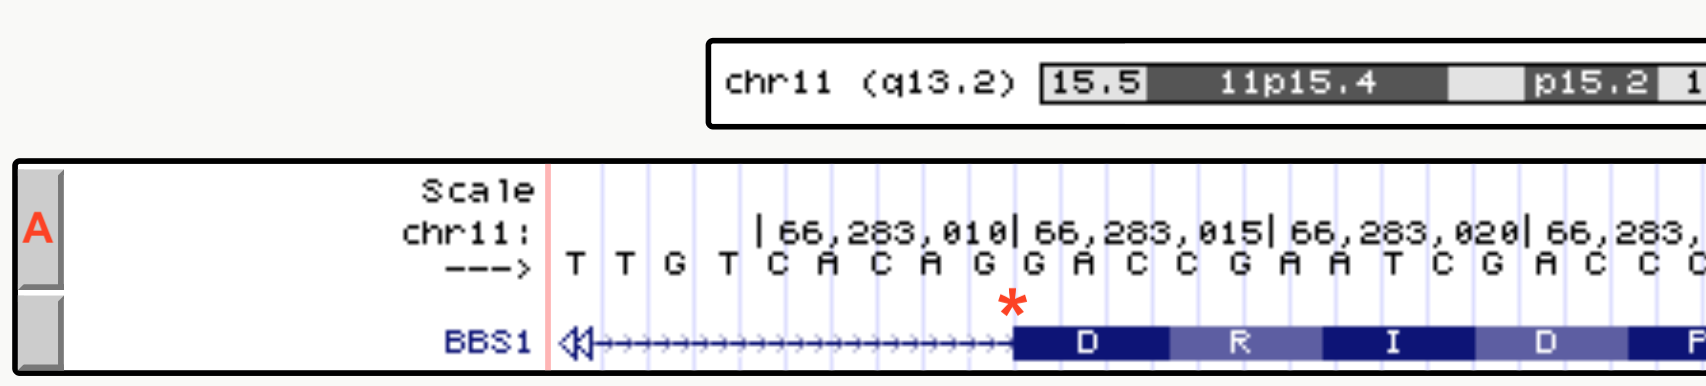
\includegraphics[width=0.5\linewidth]{static/images/BBS1zoomtosequence}

}

\caption{The drag-select tool was used to zoom in close to a small portion of an exon intron junction of BBS1. As you can see the first 4 nucleotides of the exon shown are G-A-C-C.}\label{fig:zoomtosequence}
\end{figure}

\hypertarget{test-your-understanding-1}{%
\subsection{\texorpdfstring{\href{https://forms.gle/LFvwBLFpZh5mQwiX7}{Test Your Understanding}}{Test Your Understanding}}\label{test-your-understanding-1}}

\begin{itemize}
\tightlist
\item
  \emph{What year was the most recent Human Genome Assembly uploaded to the UCSC genome browser?}
\item
  \emph{Go to the UCSC Genome Browser home page. Hover your mouse over the ``Genome Browser'' link in the toolbar at the top of the page. Choose ``Reset all User Settings'' in the pop up menu. Choose the Feb.~2009 Human Genome Assembly and click ``Go''. How many evidence tracks are displayed in the Browser window?}
\item
  \emph{Where is BBS1 located on chromosome 11, the long arm or the short arm?}
\item
  \emph{Search for the gene, SOD1. Which chromosome is it on?}
\item
  \emph{Where is SOD1 located? On the long arm or short arm of the chromosome?}
\item
  \emph{Search for the gene, ACVR1. Which chromosome is it on?}
\item
  \emph{Where is ACVR1 located? On the long arm or short arm of the chromosome?}
\item
  \emph{Fill in the blank. Have you noticed a trend? The short arm of each chromosome is always positioned on the \_\_\_\_\_\_\_?}
\item
  \emph{First, use my session link to jump to BBS1. Then use the Drag and Select tool to zoom into the beginning of exon 2 of BBS1. Continue to zoom in until you are close enough to see the genome sequence. What are the first four nucleotides?}
\end{itemize}

© 2019, Maria Gallegos. All rights reserved.

\hypertarget{an-introduction-to-gene-structure}{%
\chapter{\texorpdfstring{\emph{An Introduction to Gene Structure}}{An Introduction to Gene Structure}}\label{an-introduction-to-gene-structure}}

To follow along with the text and to answer the ``Test Your Understanding'' questions use the \href{https://genome.ucsc.edu/s/megallegos/Biol\%20310\%20Module\%201}{``BBS1 gene structure'' session} at the UCSC Genome Browser.

\hypertarget{exons-and-introns}{%
\section{Exons and Introns}\label{exons-and-introns}}

During gene expression, one continuous strand of genomic DNA is used as a template to produce a single-stranded RNA transcript. This process is called \textbf{transcription}. This RNA transcript is nearly an identical copy of of the nontemplate strand of genomic DNA\footnote{The only difference: uracil bases replace thymine bases}. In eukaryotes, internal segments of the RNA transcript are often removed. These internal segments are called \textbf{introns} (or \textbf{int}ervening \textbf{r}egi\textbf{ons}). The segments of RNA that remain are \emph{welded} back together (in order) and are called \textbf{exons} (or \textbf{ex}pressed regi\textbf{ons}). To view the exon/intron organization of the BBS1 RNA transcript, click on my named session entitled, \href{https://genome.ucsc.edu/s/megallegos/Biol\%20310\%20Module\%201}{BBS1 gene structure} and review the schematic within the NCBI RefSeq Gene Prediction Evidence Track. The BBS1 transcript consists of ``boxes'' connected by lines (Figure \ref{fig:BBS1transcript}). The boxes are exons (two examples are highlighted with a red asterix). The lines are introns (one example is highlighted with a purple asterix). Now, hover your mouse over various parts of the schematic (at the UCSC genome browser page). If you hover long enough a popup window will appear indicating which intron or exon you are pointing to!

\begin{figure}

{\centering 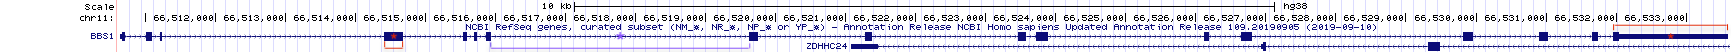
\includegraphics[width=1\linewidth]{static/images/exonintron}

}

\caption{Understanding gene prediction evidence track schematic. The boxes are exons (two examples are bracketed and highlighted with a red asterix). The lines are introns (one example is bracketed and highlighted with a purple asterix)}\label{fig:BBS1transcript}
\end{figure}

\hypertarget{test-your-understanding-2}{%
\subsection{\texorpdfstring{\href{https://forms.gle/V4fYwV2ZoiCVXfEv8}{Test your understanding}}{Test your understanding}}\label{test-your-understanding-2}}

\begin{itemize}
\tightlist
\item
  \emph{How many exons does BBS1 contain?}
\item
  \emph{How many introns does BBS1 contain?}
\item
  \emph{Which exon is the longest (as judged by eye)?}
\item
  \emph{Find SOD1 in the UCSC Genome Browser. Which SOD1 intron is the shortest (as judged by eye)?}
\end{itemize}

\hypertarget{one-gene-many-splice-variants}{%
\section{One gene, many splice variants}\label{one-gene-many-splice-variants}}

A single RNA transcipt is sometimes spliced in a variety of different ways to produce more than one unique mRNA. This is called \textbf{alternative splicing} and each mRNA produced is called a \textbf{splice variant}. Since each splice variant has the capacity to produce a unique protein or \textbf{isoform}, the 24,000 protein-coding genes present in the human genome can actually produce \emph{many more than} 24,000 unique proteins!

To see this for yourself, zoom out exactly \textbf{10X} to explore a larger section of chromosome 11\footnote{Notice that at this zoom level some exons look more like vertical lines. This is because, exons are typically shorter than introns (at least in mammals) and so at this zoom level exons look like lines instead of boxes}. Now more than one gene can be viewed in the browser window. Again, the name of each gene is given on the left side of each gene/transcript schematic. Regions of the genome that are transcribed to produce multiple mRNAs are indicated by a \emph{series} of box/line schematics that are \emph{stacked} vertically. How do I know these stacks represent a single gene? Each graphical representation in the stack has the \emph{same} gene name (Figure \ref{fig:zoom}).

\begin{figure}

{\centering 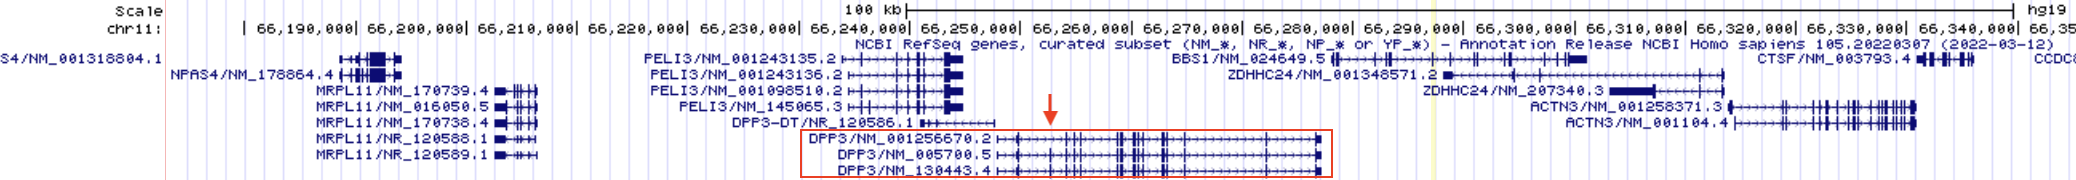
\includegraphics[width=1\linewidth]{static/images/10zoom}

}

\caption{The DPP3 gene produces three unique mRNAs. See the red box. One obvious difference is highlighted with a red arrow. The 2nd and 3rd splice form have an exon not included in the topmost splice form listed.}\label{fig:zoom}
\end{figure}

Alternative splicing is only one way multiple unique mRNAs are produced from a single region of DNA (a single gene)? There are three main methods: 1) Use of an alternative transcriptional start site (Figure \ref{fig:altinit}), 2) use of an alternative transcriptional termination site (Figure \ref{fig:altter}) and 3) alternatively splicing. For example, DPP3 begins and ends transcription at the same location but the RNA transcript that is produced is spliced in three distinct ways to produce three alternative splice forms (Figure \ref{fig:zoom}).

\begin{figure}

{\centering \includegraphics[width=1\linewidth]{static/images/altinitiation}

}

\caption{Transcription initiation for the LGALS12 gene can be found at two distinct places according to the NCBI RefSeq gene database. The red arrow points to the two transcription start sites}\label{fig:altinit}
\end{figure}

\begin{figure}

{\centering 
\includegraphics[width=1\linewidth]{static/images/alttermination}

}

\caption{Transcription termination for the TTC17 gene occurs at two different sites according to the NCBI RefSeq gene database. Each is highlighted with a red arrow}\label{fig:altter}
\end{figure}

Again, multiple mRNA isoforms from the same gene can (but don't always) produce multiple, unique protein isoforms. In some cases, these unique proteins differ enough to function distinctly. For a hilarious illustration of this concept see Figure \ref{fig:eat}.

\begin{figure}

{\centering 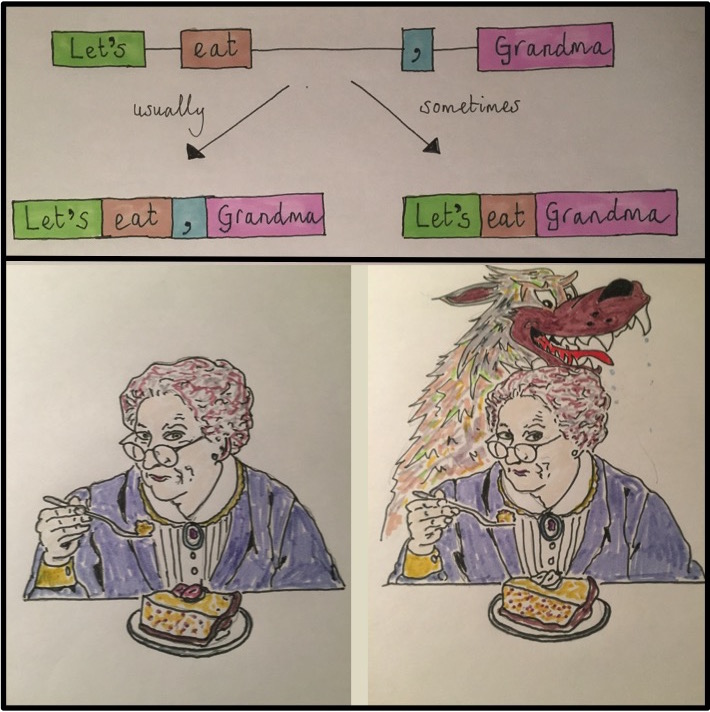
\includegraphics[width=0.5\linewidth]{static/images/eatgrandma}

}

\caption{Concept/Art by Allan James from the University of Glasgow}\label{fig:eat}
\end{figure}

\hypertarget{test-your-understanding-3}{%
\subsection{\texorpdfstring{\href{https://forms.gle/s1Ca2HyWLNyakJN38}{Test Your Understanding}}{Test Your Understanding}}\label{test-your-understanding-3}}

\begin{itemize}
\tightlist
\item
  \emph{How many unique mRNAs does PELI3 produce?}
\item
  \emph{Are the various mRNA forms produced by PELI3 the result of alternative splicing, alternative transcription initiation, alternative transcription termination or some combination?}
\item
  \emph{How many unique mRNAs does MRPL11 produce?}
\item
  \emph{Are the various mRNA forms the result of alternative splicing, alternative transcription initiation, alternative transcription termination or some combination?}
\item
  \emph{How many unique mRNAs does ACTN3 produce?}
\item
  \emph{Are the various mRNA forms the result of alternative splicing, alternative transcription initiation, alternative transcription termination or some combination?}
\end{itemize}

\hypertarget{coding-and-noncoding-exons}{%
\section{Coding and Noncoding Exons}\label{coding-and-noncoding-exons}}

The spliced transcript or messenger RNA (mRNA) is used as a template to create a polypeptide\footnote{A chain of amino acids linked together by peptide bonds. While the words ``protein'' and ``polypeptide'' are often used interchangeably, the term protein is more vague. It could refer to a single polypeptide or it might mean multiple polypeptides bound together in a complex. On the other hand, polypeptide always refers to a single sequence of amino acids}. This process is called translation and is mediated in part by the ribosome\footnote{A cytoplasmic machine (comprised of RNA and protein) which uses the mRNA to synthesize a polypeptide.}. The ribosome ``reads'' each codon\footnote{A set of three adjacent nucleotides in an mRNA molecule that specify the incorporation of an amino acid in a growing polypeptide chain or that signals the end of polypeptide synthesis. Codons with the latter function are called termination codons (Snustad).} within the mRNA to create a polypeptide. That said, an mRNA is more than just codons! In fact, codons \textbf{only occupy the central region of an mRNA}. The ends of the mRNA are called \textbf{noncoding regions} or untranslated regions (UTRs). The noncoding region at the 5' end is called the 5' untranslated region (5' UTR). While the noncoding region at the 3' end is called the 3' untranslated region (3' UTR). The transition from noncoding to coding and back to noncoding does \emph{not} coincide with exon boundaries. Thus, exons can be described as coding exons, noncoding exons or exons of mixed character. In fact, exon 1 of BBS1 is part noncoding (5' UTR) and part coding. The same is true of exon 17.

Let's see how the 5' UTR, coding and 3' UTR are illustrated in the UCSC Genome Browser. ``Drag-and-Select'' exon 1 of BBS1 until your window looks similar to Figure \ref{fig:topstrand}. You should now see the top strand of the genome sequence in the ``base position'' track. The predicted transcript begins with G-G-T-T etc. If you do not see sequence in the base position track, you have not zoomed in far enough. Zoom in farther. If you do not see the G-G-T-T sequence at the beginning of BBS1, you are in the wrong location.

How do I know this sequence is the top strand\footnote{The top strand of DNA is also referred to as the ``+ strand''} of this DNA segment? Because the arrow to the left of the genome sequence (see red Asterix, Figure \ref{fig:topstrand}) is pointing to the right (---\textgreater). In genetics and molecular biology, the blunt end of an arrow represents the 5' end of a DNA strand while the pointed end of an arrow represents the 3' end. \emph{Always}.

\begin{figure}

{\centering 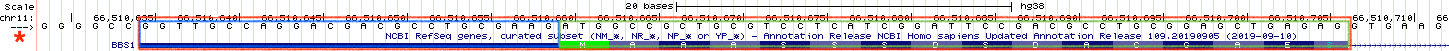
\includegraphics[width=1\linewidth]{static/images/topstrandexon1}

}

\caption{Exon 1 (red box) of BBS1 is part noncoding exon (blue box) and part coding exon (green box)}\label{fig:topstrand}
\end{figure}

At this zoom level, you should also be able to see the amino acid sequence that exon 1 codes for (Figure \ref{fig:topstrand}: M-A-A-A-S-S-S-D-S-D-A-C-G-A-E-S. Notice that the amino acid sequence does not start at the beginning of exon 1. Moreover, the noncoding portion of exon 1 is also not drawn as thick as the coding portion of exon 1. This thinner portion of exon 1 is the 5' untranslated region (5' UTR). This is because it contains no codons (it is noncoding) AND it is the 5' end of BBS1.

\hypertarget{test-your-understanding-4}{%
\subsection{\texorpdfstring{\href{https://forms.gle/DaZ8kh1EH7Bqi6Fr7}{Test your understanding}}{Test your understanding}}\label{test-your-understanding-4}}

\begin{itemize}
\tightlist
\item
  \emph{How long is the 5' UTR of BBS1 (manually count the number of nucleotides)?}
\item
  \emph{Consider this arrow: \textless--- representing a single strand of DNA. Is the 3' end of this DNA on the right or left?}
\item
  \emph{Search for the gene, MDM4 in the UCSC Genome Browser. What type of exon is exon 1 (noncoding, coding or both - of mixed character)?}
\end{itemize}

To view the entire BBS1 gene again, click on the named session link for \href{https://genome.ucsc.edu/s/megallegos/Biol\%20310\%20Module\%201}{BBS1 Gene Structure}. Notice the box representing the last exon of BBS1 also consists of both a thick and thin portion. The thin portion at the end of the BBS1 gene is also noncoding. Since this is the 3' end of BBS1, this portion of BBS1 is called the 3' untranslated region or 3' UTR. Now ``Drag-and-Select'' the \textbf{coding} portion of the last exon. If your view does not look like (Figure \ref{fig:lastexon}), you may have selected the \textbf{entire} last exon when you should have just selected the \textbf{coding} portion of the last exon. See the difference? Now you can clearly see that the amino acid sequence stops before the end of the last exon and the exon schematic transitions from thick to thin. NOTE: The stop codon is represented by an asterix. In many genes, the first and last exons consist of both noncoding and coding sequence while the central exons are coding only. As you explore more of the genome, you will see there are exceptions. Sometimes the \emph{first few} exons and/or the \emph{last few} exons are completely noncoding!

\begin{figure}

{\centering 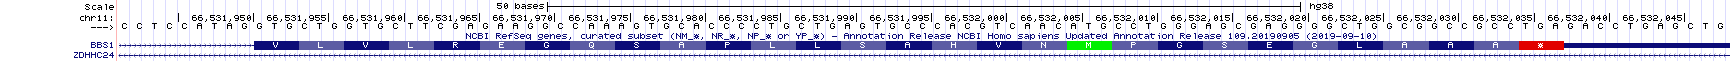
\includegraphics[width=1\linewidth]{static/images/lastcodingexon}

}

\caption{The coding portion of the last exon of BBS1}\label{fig:lastexon}
\end{figure}

\hypertarget{coding-exons-determine-protein-sequence}{%
\section{Coding Exons Determine Protein Sequence}\label{coding-exons-determine-protein-sequence}}

Polypeptides are a series of amino acids held together by peptide bonds. The amino acid sequence is determined by the order of codons present in the central portion of a mature mRNA, the coding exons. Each codon consists of a group of three consecutive bases. Since there are four nucleotides total (G, A, T and C), the equation, 4\^{}3, indicates that there are 64 possible codons. Most of the 64 codons code for an amino acid. Three do not and therefore act as STOP signals also known as termination codons. Figure \ref{fig:geneticcode} is one way to display the genetic code. In this graphic, codons are read from the \textbf{center} out to the periphery (from 5' to 3'). For example, G-C-A codes for Alanine. Ala and A are the standard three letter and single letter codes, respectively. In this genetic code, Uracil replaces Thymine as ribosomes scan mRNA molecules not DNA.

\begin{figure}

{\centering 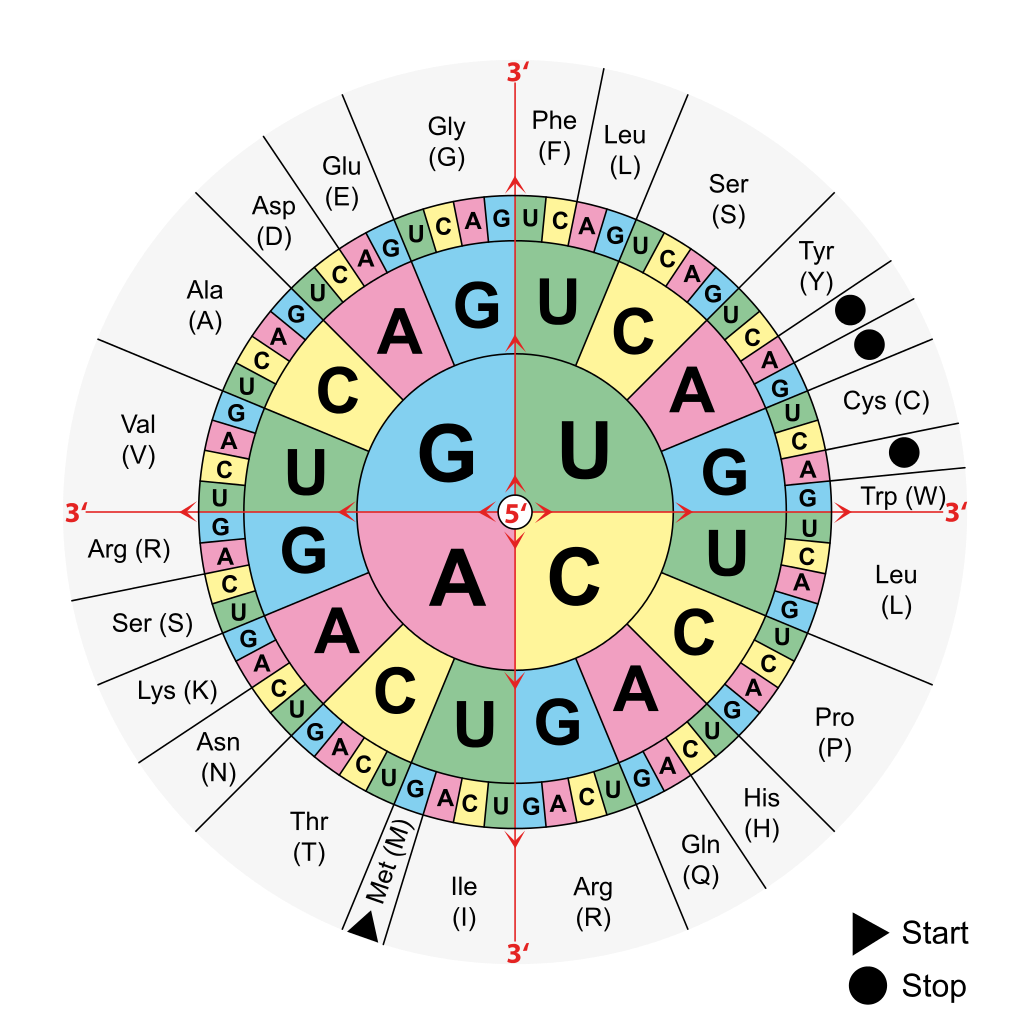
\includegraphics[width=0.75\linewidth]{static/images/circulargeneticcode}

}

\caption{[Image from wikipedia](https://commons.wikimedia.org/wiki/File:Aminoacids_table.svg)}\label{fig:geneticcode}
\end{figure}

Use whatever method you'd like to get back to a close-up view of exon 1 of BBS1 Figure \ref{fig:topstrand}. Notice that the first amino acid of the protein is a methionine (M) and is shaded in green. In fact, the first amino acid of all proteins should be methionine as the A-U-G codon is the start codon in most cases. You can confirm that this is true for BBS1 by looking at the three nucleotides positioned directly above the ``M'' (You should see ATG since you are viewing genomic DNA). The second codon is G-C-C. The third codon is G-C-T. Both code for Alanine (Ala, A).

In BBS1, it is clear that the codons are read from left to right in non-overlapping groups of three nucleotides. Since the codons are found in the top strand, you can also say that these codons are read from 5' to 3'. In fact, codons are always read from 5' to 3' in non-overlapping, groups of three nucleotides. Now let's re-examine the last \textbf{coding} exon of BBS1 (Figure \ref{fig:lastexon}. Notice that the stop codon at the end of BBS1 is represented by an ``*'' and highlighted in red.

\hypertarget{test-your-understanding-5}{%
\subsection{\texorpdfstring{\href{https://forms.gle/LUjW3ngaerH1ipeV6}{Test your understanding}}{Test your understanding}}\label{test-your-understanding-5}}

The codons below are written as a DNA sequence from 5' on the left to 3' on the right (5' to 3'). Use the genetic code found in Figure \ref{fig:geneticcode} to answer the top three questions (open in a new tab). Use the UCSC genome browser to answer the remaining questions.

\begin{itemize}
\tightlist
\item
  \emph{What amino acid does the codon, CGG, code for?}
\item
  \emph{What amino acid does the codon, TTC, code for?}
\item
  \emph{What amino acid does the codon, CAT, code for}
\item
  \emph{Write out the DNA sequence of the 5th codon for BBS1}
\item
  \emph{What does the 5th codon of BBS1 code for?}
\item
  \emph{Write out the DNA sequence of the 8th codon for BBS1}
\item
  \emph{What does the 8th codon of BBS1 code for?}
\item
  \emph{Write out the DNA sequence of the stop codon for BBS1}
\item
  \emph{EXTRA CREDIT! Write out the DNA sequence of the 16th codon}
\end{itemize}

\hypertarget{top-strand-and-bottom-strand-genes}{%
\section{Top strand and bottom strand genes}\label{top-strand-and-bottom-strand-genes}}

We learned in the last section that the codons for BBS1 can be read from within the top strand (+ strand) and they are read from left to right. For BBS1, this means that the top strand is the sense strand while the bottom strand is the template strand\footnote{For BBS1, the bottom strand is used as the template for transcription and by definition is complementary to the top strand}. Sometimes the sense strand is also called the nontemplate strand. \textbf{That said, the sense strand of a gene is not ALWAYS the top strand in a genome browser}. Click on the Named Session for \href{https://genome.ucsc.edu/s/megallegos/Biol\%20310\%20Module\%201}{BBS1 Gene Structure} then zoom out 3X to look at BBS1 and its neighboring genes. Your NCBI Refseq gene track should look something like (Figure \ref{fig:neighboringgenes}).

\begin{figure}

{\centering 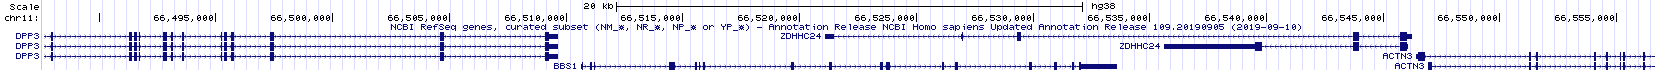
\includegraphics[width=1\linewidth]{static/images/neighboringgenes}

}

\caption{BBS1 and its neighboring genes. BBS1 is flanked by DPP3 on the left and ZDHHC24 on the right. DPP3 is upstream. ZDHHC24 is downstream. Click on the image to enlarge. Click again to resume reading.}\label{fig:neighboringgenes}
\end{figure}

Now ``Drag-and-Select'' the first half of BBS1 to zoom in somewhat. Notice there are ``orientation wedges'' spaced regularly along all introns ((Figure \ref{fig:orientationwedges}). They are either oriented to the right (red box) or to the left (green box). These ``orientation wedges'' indicate the orientation of the gene on the chromosome. They tell you where the 5' end of the gene is and they indicate which strand of chromosomal DNA is the sense strand for a given gene (top or bottom, + or -).

\begin{figure}

{\centering 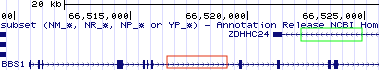
\includegraphics[width=0.6\linewidth]{static/images/orientationwedges}

}

\caption{The orientation wedges are visible within introns. When they point to the right (red box), the beginning of the gene is on the left and the gene is a top strand gene (plus strand). When they point to the left (green box), the beginning of the gene is on the right and the gene is a bottom strand gene (minus strand).}\label{fig:orientationwedges}
\end{figure}

When the orientation wedges point to the right, ``) ) ) )'' (i.e.~see BBS1),

\begin{enumerate}
\def\labelenumi{\arabic{enumi}.}
\tightlist
\item
  The beginning of the gene is on the left.
\item
  The top strand (+ strand) is the sense strand (nontemplate strand)
\item
  the bottom strand (- strand) is the template strand.
\end{enumerate}

When the orientation wedges point to the left, ``( ( ( ('', the reverse is true (i.e.~see ZDHHC24),

\begin{enumerate}
\def\labelenumi{\arabic{enumi}.}
\tightlist
\item
  The beginning of the gene is on the right.
\item
  The top strand (+ strand) is the template strand.
\item
  The bottom strand (-strand) is the sense strand (nontemplate strand)
\end{enumerate}

These orientation wedges not only represent the orientation of the gene on the chromosome but also the direction of transcription. The beginning of a gene (the 5' end) is always transcribed first. RNA polymerase, the enzyme that catalyzes RNA transcription, moves from the beginning of the gene towards the end of the gene. Thus, for BBS1, RNA polymerase moves from left to right using the bottom strand as a template. For ZDHHC24, RNA polymerase moves from right to left using the top strand as a template!

\hypertarget{test-your-understanding-6}{%
\subsection{\texorpdfstring{\href{https://docs.google.com/forms/d/e/1FAIpQLScgFkZWsytBOOLiaJeJi8fTler4YYHuWkDosv5gGORJIneT0w/viewform?usp=sf_link}{Test your understanding}}{Test your understanding}}\label{test-your-understanding-6}}

To answer the following set of questions, go to my \href{https://genome.ucsc.edu/s/megallegos/Biol\%20310\%20Module\%201}{BBS1 Gene Structure named session} then zoom out 10X.

\begin{itemize}
\tightlist
\item
  \emph{How are the various mRNA forms produced by the ZDHHC24 gene? Do they result from alternative splicing, transcription initiation, transcription termination or a combination of these events?}
\item
  \emph{Which strand (top or bottom) is the sense strand for ACTN3?}
\item
  \emph{Where is the beginning of the ACTN3 gene as displayed in the browser, on the left or right?}
\item
  \emph{Which direction does RNA polymerase travel along genomic DNA during transcription of ACTN3 (as displayed in the browser), to the left or to the right?}
\item
  \emph{Which strand (top or bottom) is the sense strand for DPP3?}
\item
  \emph{Where is the beginning of the DPP3 gene as displayed in the browser, on the left or right?}
\item
  \emph{Which direction does RNA polymerase travel along DPP3 during transcription (as displayed in the browser), to the left or to the right?}
\item
  \emph{Which strand (top or bottom is the sense strand for CTSF?}
\item
  \emph{Where is the beginning of the CTSF gene, on the left or right as displayed in the browser?}
\item
  \emph{Which direction does RNA polymerase travel along CTSF during transcription (as displayed in the browser), to the left or to the right?}
\end{itemize}

Now let's look at the beginning of the first coding exon for ZDHHC24 up close. First, click on my named session for \href{https://genome.ucsc.edu/s/megallegos/Biol\%20310\%20Module\%201}{BBS1 Gene Structure} then zoom out 3X to find the \textbf{beginning} of ZDHHC24. ``Drag-and-Select'' as many times necessary to zoom to the \textbf{first} half of the \textbf{first coding exon} for ZDHHC24. Your ``NCBI Refseq Gene Track should look something like Figure \ref{fig:firstcodingexonZDHHC24}. If not, you may have zoomed into the first half of exon 1 which is noncoding. Or maybe you are at the wrong end of the gene! Make sure you understand what went wrong and how to find the right spot.

\begin{figure}

{\centering 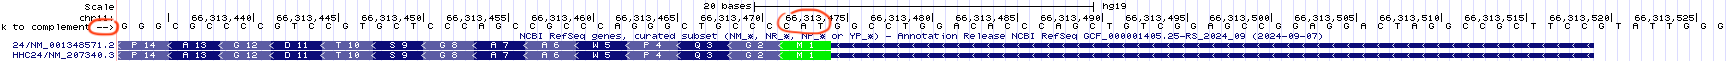
\includegraphics[width=1\linewidth]{static/images/firstcodingexonZDHHC24}

}

\caption{This is the first half of the first **coding** exon of ZDHHC24. The noncoding portion of exon 1 extends to the right this time because *ZDHHC24* is a bottom strand (or minus strand) gene. The red oval highlights the strand you are currently viewing. Since the arrow points to the right, the top strand (5' on the left) is displayed. You can toggle this arrow with your mouse.}\label{fig:firstcodingexonZDHHC24}
\end{figure}

\begin{figure}

{\centering \includegraphics[width=1\linewidth]{static/images/firstcodingexonZDHHC24bottom}

}

\caption{Again, this is the first half of the first **coding** exon of ZDHHC24. The red oval highlights the strand you are currently viewing. Since the arrow points to the left, the bottom strand (5' on the right) is displayed. Notice that the DNA sequence is gray. Compare to the top image. This is a visual reminder of which strand you are viewing.}\label{fig:firstcodingexonZDHHC24bottom}
\end{figure}

Look at the three nucleotides centered above the Methionine (colored in green on the right side of Figure \ref{fig:firstcodingexonZDHHC24}). Notice that the nucleotides listed from left to right is NOT an A-T-G as you might expect but instead C-A-T! This is because you are ``reading'' the top strand of DNA. ZDHHC24 is a \textbf{bottom} strand gene. To view the bottom strand of DNA, click on the far left arrow within the Base Position Track (See the red oval, Figure \ref{fig:firstcodingexonZDHHC24}). Notice the orientation of the arrow will flip and the genome sequence in your ``Base Position'' Track will transform into light gray (red oval, \ref{fig:firstcodingexonZDHHC24bottom}). Now there is an A-T-G directly above the Methionine (M) but instead of reading it from left to right, you must read it from right to left! This is because the bottom strand is oriented with 5' end on the right. \textbf{You ALWAYS read and write sequence from 5' to 3'}.

\hypertarget{test-your-understanding-7}{%
\subsection{\texorpdfstring{\href{https://docs.google.com/forms/d/e/1FAIpQLSeaojvlNdLiH-VjdFQA-tjv3U3-f8dCK1mZA2n4KQXwoCI5NQ/viewform?usp=sf_link}{Test your understanding}}{Test your understanding}}\label{test-your-understanding-7}}

\begin{itemize}
\tightlist
\item
  \emph{Write out the DNA sequence of the 3rd codon for ZDHHC24 (Always write sequence from 5' to 3').}
\item
  \emph{Write out the DNA sequence of the 5th codon for ZDHHC24.}
\item
  \emph{Write out the DNA sequence of the stop codon used by the \textbf{short} mRNA form of ZDHHC24.}
\item
  \emph{Write out the DNA sequence of the stop codon used by the \textbf{long} mRNA form of ZDHHC24 (Notice: the stop codon is not always in the last exon!).}
  HINT: To confirm that you have chosen your codon sequence correctly, use the \href{https://commons.wikimedia.org/wiki/File:Aminoacids_table.svg}{genetic code} to confirm that the codon you chose codes for the amino acid found at that position in the gene (NOTE: In general, genetics substitute U for T).
\end{itemize}

Don't forget, DNA is double-stranded. The two DNA strands anneal (hybridize) in an \textbf{antiparallel} orientation. The 5' end of the top strand is on the left. The 5' end of the bottom strand is on the right. Some genes, like BBS1 create an RNA transcript with a sequence that matches the top strand. Other genes, like ZDHHC24, create an RNA transcript with a sequence that matches the bottom strand.

\hypertarget{reading-frames}{%
\section{Reading Frames}\label{reading-frames}}

A reading frame begins with a start codon. This is the first codon ``read'' by the ribosome. All subsequent codons are read in \textbf{nonoverlapping groups} of three. Thus, the start codon ``sets'' the reading frame. A reading frame ends only when a stop codon is encountered that is in the same reading frame as the start codon. This is the last codon ``read'' by the ribosome.

Imagine you isolate and sequence a short random stretch of DNA pulled from the ocean. It is likely genomic DNA and you want to see if corresponds to a coding portion of a gene. Specifically, you want to see if this short stretch of DNA codes for a previously studied protein. Of course, you have no clue which strand might be used as a template for transcription nor where the start codon is. Here is a thought question: \textbf{\emph{What is the maximum number of unique polypeptides that a single segment of double-stranded DNA could theoretically produce?}} Your answer will be revealed below.

To view all possible reading frames associated with a given segment of DNA zoom into to the first exon of BBS1. Next, right click on the grey rectangle corresponding to the Base Position track (See arrow, Figure \ref{fig:basepositiondense}). A pop-up menu will appear. Choose ``full''.

\begin{figure}

{\centering 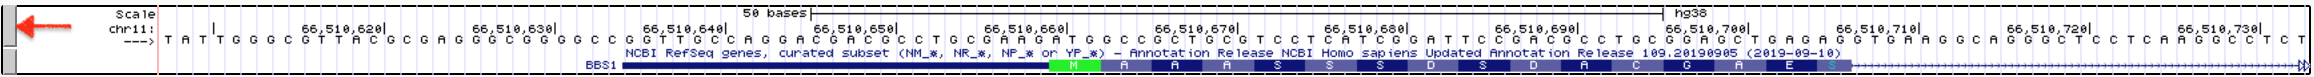
\includegraphics[width=1\linewidth]{static/images/basepositiondense}

}

\caption{How to view all three reading frames for a single strand of DNA. Right click on the gray rectangle on the left of the Base Position Track (red arrow). A pulldown menu will open. Choose Full.}\label{fig:basepositiondense}
\end{figure}

You should now see three reading frames displayed below the nucleotide sequence. Why three? This is the maximum number of unique polypeptides that can be theoretically produced from a given segment of the top strand of DNA. See what happens when you toggle to the bottom strand of DNA (click the arrow ---\textgreater{} on the far left of the DNA sequence). Now you can view the three reading frames that correspond to the bottom strand of DNA. Both views are shown one on top of the other in Figure \ref{fig:basepositionfullreverse}. Notice they are different.

\begin{center}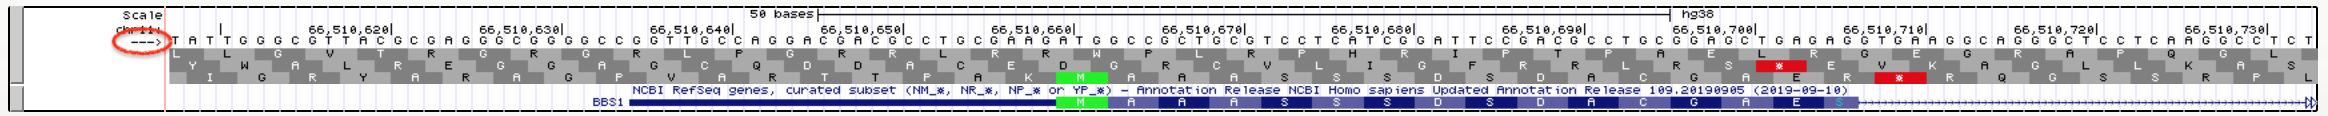
\includegraphics[width=1\linewidth]{static/images/basepositionfull} \end{center}

\begin{figure}

{\centering 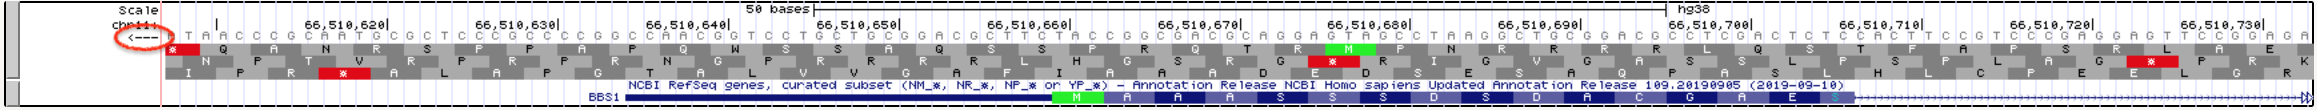
\includegraphics[width=1\linewidth]{static/images/basepositionfullreverse}

}

\caption{Once you change the base position track to **Full**, the three possible reading frames for a *single* DNA strand will be displayed. When the arrow points to the right, the three reading frames will be of the top strand (top image). Notice the start codon in green matches the start codon in the third reading frame and nearly all of the amino acids in exon one match the amino acids in the third reading frame. This is because *BBS1* is a top strand gene and we are viewing the three reading frames for the top strand. Now when the arrow points to the left, the three reading frames are for the bottom strand (bottom image). Now *none* of the amino acids in the three reading frames match the amino acids found in *BBS1*}\label{fig:basepositionfullreverse}
\end{figure}

The three reading frames corresponding to the top strand are numbered +1 (top), +2 (middle) and +3 (bottom). The three reading frames corresponding to the bottom strand (when shown) are numbered -1 (top), -2 (middle) and -3 (bottom). For convenience, the position of all possible start codons are highlighted in green and all possible stop codons (*) are highlighted in red.

Now, zoom out until you can see the first three exons of BBS1 (Figure \ref{fig:threeexons}). At this level of zoom, you should still be able to read the amino acid sequence within the gene schematic \emph{and} within the base position track. Notice there are many ``start'' and ``stop'' codons scattered throughout this segment of the genome (red and green boxes). This should not be surprising given that start and stop codons are only three nucleotides in length and they would simply occur by chance. \textbf{The ability of an ATG or TGA, TAA, TAG to function as a start or stop codon, respectively, depends on context}. For example, the real start codon for a given gene is typically the first start codon encountered in an mRNA as the Ribosome scans the mRNA from 5' to 3' (more about this later).\\

\begin{figure}

{\centering 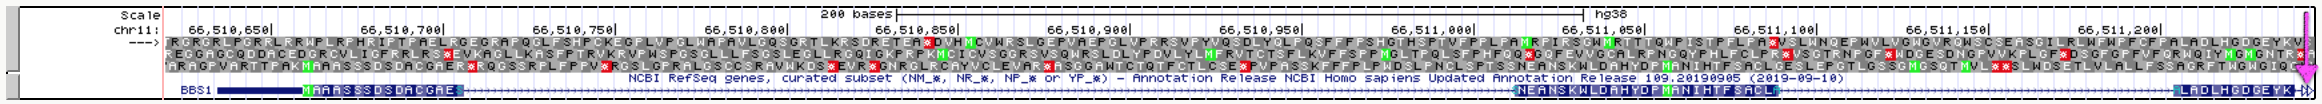
\includegraphics[width=1\linewidth]{static/images/firstthreeexons}

}

\caption{All ATG codons are colored green regardless if they function as a start codon or not. Similarly, all TGA, TAA and TAG codons are colored red regardless if they function as a stop codon. How these triplets function depends on context.}\label{fig:threeexons}
\end{figure}

Now, notice that the amino acid sequence within the BBS1 gene schematic always matches \textbf{one} of the three reading frames. For our example, the coding portion of exon 1 begins with a methionine (highlighted in green). The +3 reading frame also has a methionine in this same position. Compare a few more amino acids in BBS1 and the +3 reading frame. You should see that all match (except one). Thus, coding exon 1 utilizes the +3 reading frame! By the way, do you see the exception?

Which reading frame do the other coding exons utilize? Is it always the same reading frame? Or does it change from exon to exon. New trick: To easily view exons farther downstream (3' of), click on the open arrow head on the far right (See hot pink arrow at the far right of the image, Figure \ref{fig:threeexons}). Also, if you hover over the open triangle and don't click, a small pop up will appear with information about which exon you are jumping to! This may come in handy while answering the following questions.

\hypertarget{test-your-understanding-8}{%
\subsection{\texorpdfstring{\href{https://docs.google.com/forms/d/e/1FAIpQLSckMbKa16Rv7ZEFuQNP8Q1joHgU04UJx-oHZznrnbpaBOAqcQ/viewform?usp=sf_link}{Test your understanding}}{Test your understanding}}\label{test-your-understanding-8}}

Recall: The three reading frames corresponding to the top strand (plus strand) are called +1 (top), +2 (middle) and +3 (bottom). The three reading frames corresponding to the bottom strand (minus strand) are called -1 (top), -2 (middle) and -3 (bottom). Answer the following questions about BBS1 (a top strand gene) and ZDHHC24 (a bottom strand gene).

\begin{itemize}
\tightlist
\item
  \emph{Which reading frame does exon 2 of BBS1 use?}
\item
  \emph{Which reading frame does exon 3 of BBS1 use?}
\item
  \emph{Which reading frame does exon 4 of BBS1 use?}
\item
  \emph{Which reading frame does exon 5 of BBS1 use?}
\item
  \emph{Which reading frame does exon 1 of the long form of ZDHHC24 use?}
\item
  \emph{Which reading frame does exon 2 of the long form of ZDHHC24 use?}
\item
  \emph{Which reading frame does exon 3 of the long form of ZDHHC24 use?}
\item
  \emph{Which reading frame does exon 4 of the long form of ZDHHC24 use?}
\item
  \emph{Review your answers above. Are the reading frames used by BBS1 the same for each exon examined? Are the reading frames used by ZDHHC24 the same for each exon examined?}
\end{itemize}

\hypertarget{how-to-view-and-retrieve-gene-product-sequences}{%
\section{How to View and Retrieve Gene Product Sequences}\label{how-to-view-and-retrieve-gene-product-sequences}}

To retrieve BBS1 gene product sequences (or any gene product sequence) from the UCSC genome browser, click on the schematic for the BBS1 transcript in the ``Gene and Gene Predictions track''. The top half of the new page contains numerous links to pages that provide sequence information associated with this gene (Figure \ref{fig:geneinfo}). For example, to view information specifically about the BBS1 mRNA, click on the NM\_024649.5 link. To view information specifically about the protein sequence, click on the NP\_078925.3 link. NM\_024649.5 and NP\_078925.3 are known as accession codes. Accession codes that begin with NM\_ correspond to mRNA sequences. While those that begin with NP\_ correspond to protein sequences. Both sequence pages are in so-called ``Genbank format''. This format includes useful annotations that can be ``read'' by sequence analysis software programs. The mRNA or protein sequence is at the very bottom of the page. Scroll down. Alternatively, click the ``FASTA'' link to see the sequence in a simpler format. One thing you might notice: There are no uracil bases (U) in the mRNA sequence! Sequence databases do not expend any computational energy to convert thymines (T) to uracils (U) for display purposes only.

Finally, to get an overview of how BBS1 mRNA aligns with the genomic sequence, click on the ``View details of parts of alignment within browser window''. Read the text to determine what highlighting means although you may be able to deduce their meaning.

\begin{figure}

{\centering 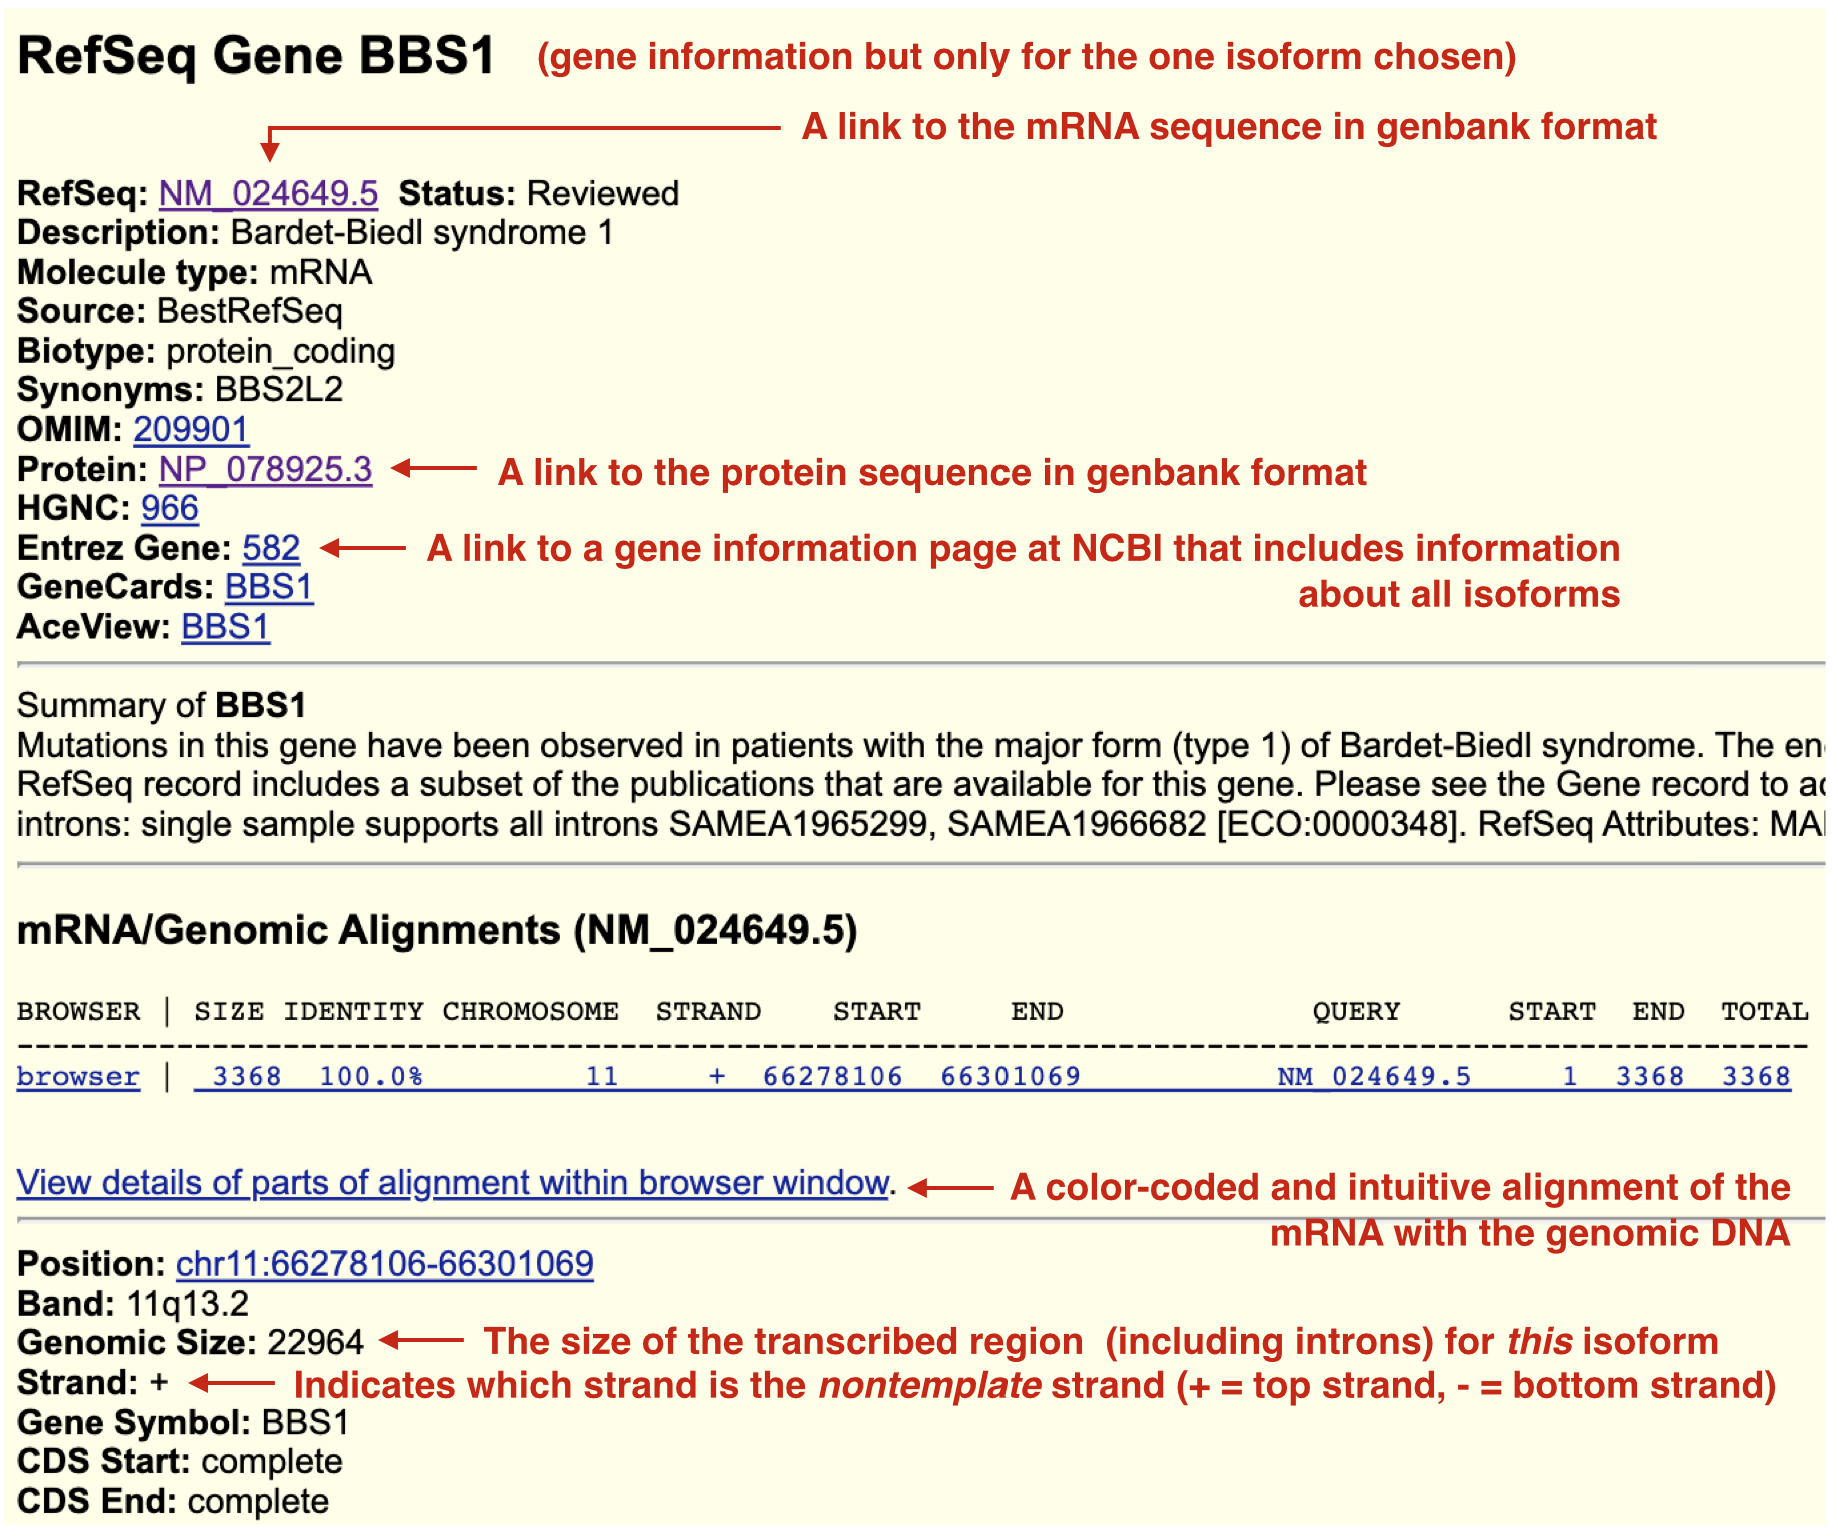
\includegraphics[width=1\linewidth]{static/images/GeneInformationPage}

}

\caption{When you click on a gene/transcript schematic in the gene prediction track you are taken to its gene information page. BBS1 only has one isoform and so there is only one gene information page. In other words, this information is transcript specific and depends on which isoform you click on. Useful links are highlighted. Some links will help you answer Test Your Understanding questions. Explore!}\label{fig:geneinfo}
\end{figure}

\hypertarget{test-your-understanding-9}{%
\subsection{\texorpdfstring{\href{https://docs.google.com/forms/d/e/1FAIpQLSdHCmDq82g5JPHIwzBtboqVw0SHCKUhkeLTWn-ZFTriPWsrhA/viewform?usp=sf_link}{Test Your Understanding}}{Test Your Understanding}}\label{test-your-understanding-9}}

\begin{itemize}
\tightlist
\item
  \emph{List the first four nucleotides of the BBS1 mRNA according to the accession record, NM\_024649.5 (Answer found in FASTA or Genbank format).}
\item
  \emph{How long (in bp) is the BBS1 spliced transcript (mRNA) according to the accession record, NM\_024649.5 (Answer found in Genbank format only)?}
\item
  \emph{List the first four amino acids of the BBS1 protein according to the accession record, NP\_078925.3 (Answer found in FASTA or Genbank format).}
\item
  \emph{How long (in amino acids) is the protein according to the accession record, NP\_078925.3 (Answer found in Genbank format only)?}
\item
  \emph{In general, what is the difference between FASTA and Genbank formats?}
\item
  \emph{EXTRA CREDIT!!! How long is the BBS1 unspliced transcript (the pre-mRNA)? (HINTS:You will find this information in the gene information page for BBS1 although you will not find the phrase ``unspliced transcript'' there. That said, the length of the unspliced transcript is equivalent to the length of the \_\_\_\_\_\_\_)}
\end{itemize}

\hypertarget{for-discussion}{%
\section{\texorpdfstring{\href{https://docs.google.com/forms/d/e/1FAIpQLSe7zNC1r8-TAGZXSN2-4BIDmX8gZ93CDlUUW0xzxQoiJVJcJA/viewform?usp=sf_link}{For Discussion}}{For Discussion}}\label{for-discussion}}

\begin{figure}

{\centering 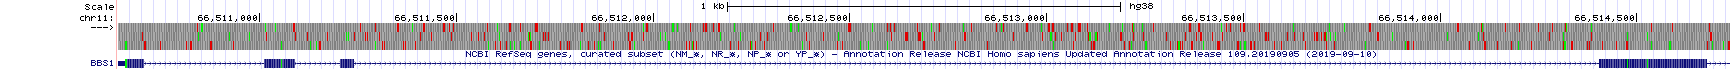
\includegraphics[width=1\linewidth]{static/images/exonsOnetoFour}

}

\caption{The first four exons of *BBS1* with the base position track set to full. All ATG codons are displayed in green. All stop codons are displayed in red.}\label{fig:fourexons}
\end{figure}

Figure \ref{fig:fourexons} above is focused on the first four exons of BBS1. It is formatted to display the three reading frames associated with the top strand. To see this section of BBS1 within the UCSC Genome Browser, click \href{https://genome.ucsc.edu/s/megallegos/FirstFourExons}{here}. Use the image or link to answer the following questions:

\begin{itemize}
\tightlist
\item
  \emph{What do you notice in general about the distribution of stop codons in introns? To see if there is a pattern, count the number of stop codons in each reading frame (+1, +2 and +3) within intron 1. Then do the same thing for intron 2 and so on. You are looking for trends. If you don't see any trends, you can review more introns and exons for BBS1.}
\item
  \emph{What do you notice in general about the distribution of stop codons in exons? To see if there is a pattern, count the number of stop codons in each reading frame (+1, +2 and +3) within exon 1. Then do the same thing for exon 2 and so on. Again, you are looking for trends.}
\item
  \emph{Do the same type of analysis but for start codons\footnote{I call them start codons but I really mean ATG codons. The only true start codon is the one where translation initiation begins. All others are simply codons for methionine. That said, all ATG codons are colored green}. Is the distribution pattern you observe for start codons similar or different than the pattern observed for stop codons?}
\end{itemize}

If you created a graph or table (in excel or by hand) to answer this, take a picture and save it. You can upload it \textbf{here}\footnote{link will appear shortly!} for extra credit.

\hypertarget{addendum}{%
\section{Addendum}\label{addendum}}

Now that you have more familiarity with gene structure, the following tutorials are highly recommended. They were created by the UCSC Genome Browser team. These are also worth revisiting before you embark on your \textbf{Independent Project} at the end of the term.

\begin{itemize}
\tightlist
\item
  \href{https://www.youtube.com/watch?v=NBDMNv2KFik\&feature=youtu.be\&list=UUQnUJepyNOw0p8s2otX4RYQ}{UCSC Genome Browser Basics. Part 1: Getting around in the Browser}
\item
  \href{https://www.youtube.com/watch?v=cYys5iXN0NY\&feature=youtu.be\&list=UUQnUJepyNOw0p8s2otX4RYQ}{UCSC Genome Browser Basics, Part 2: Configuring the Browser}
\item
  \href{https://www.youtube.com/watch?v=I25Q136d6NU\&feature=youtu.be\&list=UUQnUJepyNOw0p8s2otX4RYQ}{UCSC Genome Browser Basics. Part 3: Configuration + DNA navigation}
\item
  \href{https://www.youtube.com/watch?v=d5rHBLXwraM\&feature=youtu.be\&feature=player_detailpage\&v=8ATcoDTOc0g\&list=UUQnUJepyNOw0p8s2otX4RYQ}{Saving and Sharing Sessions on the UCSC Genome Browser}
\item
  \href{https://www.youtube.com/watch?v=jKix2B3hwnw\&feature=youtu.be\&feature=player_detailpage\&v=8ATcoDTOc0g\&list=UUQnUJepyNOw0p8s2otX4RYQ}{Controlling the visibility of data tracks on the UCSC Genome Browser}
\item
  and there is \href{https://genome.ucsc.edu/training/}{more}!
\end{itemize}

© 2019, Maria Gallegos. All rights reserved.

\hypertarget{gene-discovery-with-rna-seq}{%
\chapter{\texorpdfstring{Gene Discovery with \emph{RNA-seq}}{Gene Discovery with RNA-seq}}\label{gene-discovery-with-rna-seq}}

In this chapter, you will learn how RNA sequencing can be used to determine where genes are located in the genome. To follow along with the text and to answer the ``Test Your Understanding'' questions, start with the \href{https://genome.ucsc.edu/s/megallegos/Biol\%20310\%3A\%20Module\%202\%20RNA\%2Dseq}{``RNA-seq'' session} at the UCSC Genome Browser. You can also use this link as a starting point to view RNA-seq data for any gene of interest.

\hypertarget{gene-expression-reviewed}{%
\section{Gene expression Reviewed}\label{gene-expression-reviewed}}

For a cell to utilize a gene it must be \emph{expressed}. When it is expressed, it is either transcribed to produce a functional RNA (i.e.~tRNA) or transcribed \emph{and} translated to produce a functional polypeptide (i.e.~actin). In both cases, the first step in producing a gene product is \emph{ALWAYS} transcription. It logically follows that if you extract RNA from a cell, sequence it then find the regions in the genome with matching sequence, you have discovered regions of the genome that have been transcribed. Regions of the genome that are transcriptionally active pinpoint the position of genes. The most important take home message for this chapter: \textbf{\emph{RNA sequence provides important physical evidence to identify and locate genes in the genome}}.

\hypertarget{rna-seq}{%
\section{RNA-seq}\label{rna-seq}}

RNA sequencing allows one to determine which segments of the genome are transcriptionally active and thus serves as evidence for the existence of genes. The basic steps involved in RNA sequencing are outlined in Figure \ref{fig:rnaseq} with the focus on a single gene. In brief, mRNA is extracted from cells, fragmented into pieces then converted into double-stranded DNA (Figure \ref{fig:rnaseq}, see \emph{in vitro}). These short DNA fragments are then sequenced and computationally aligned to the genome sequence. Notice that the sequence reads only align to the exon portions of this gene in the genome. This is because mRNA was sequenced. mRNA typically contain intron sequences (see \emph{in vivo}\footnote{``in vivo'' is a Latin phrase biologists use to describe a process taking place inside a living organism (online dictionary)}). Conversion of mRNA to DNA \emph{typically} occurs after splicing is complete although sometimes intron fragments are sequenced.

\begin{figure}

{\centering 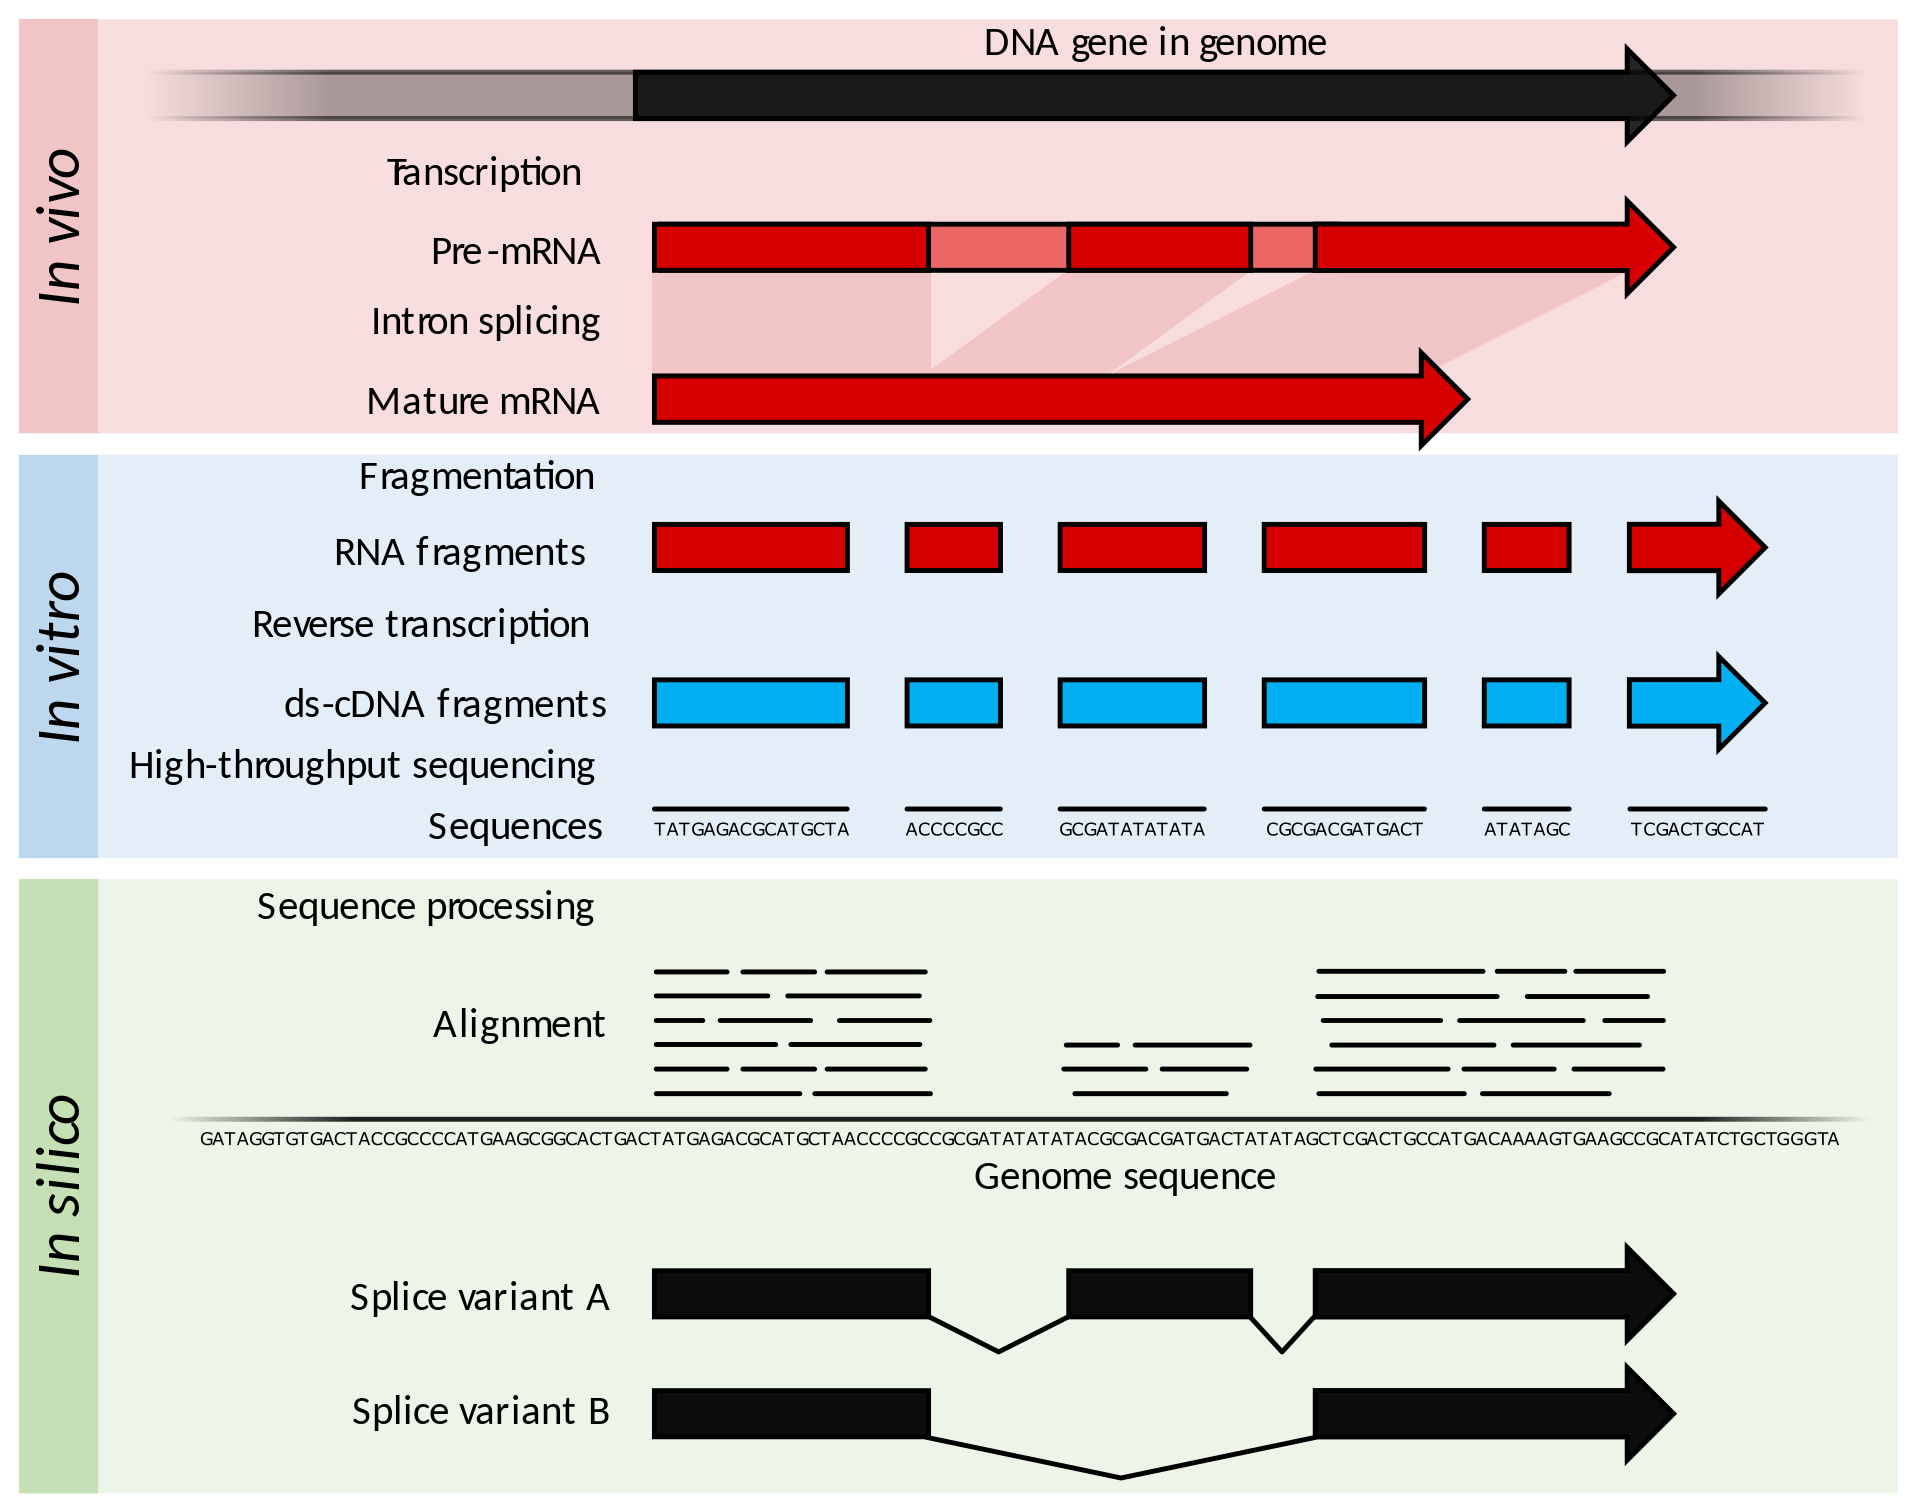
\includegraphics[width=1\linewidth]{static/images/rnaseqoutline}

}

\caption{Source: [Wikipedia](https://en.wikipedia.org/wiki/RNA-Seq)}\label{fig:rnaseq}
\end{figure}

Again, when mRNA is specifically collected for RNA-seq, this technique specifically identifies \emph{protein coding genes}. It also identifies exon-intron boundaries since introns are absent in mRNA and thus not sequenced\footnote{That said, it is impossible to remove \emph{all} pre-mRNA and so introns are occasionally sequenced as you will see when you examine the RNA seq data}. To enrich for mRNA, one can exploit one of two features unique to mRNA: All mRNAs possess a 5' cap structure and a 3' poly A tail (a string of adenines).

Figure \ref{fig:rnaextraction} demonstrates how the poly A tail can be used to purify mRNA from total RNA\footnote{\textbf{Total RNA} includes all the RNA molecule types that are found in cells. Total RNA includes mRNA (the only RNA type that is loaded into ribosomes and translated to make protein) and a wide variety of functional RNAs (i.e.~tRNA, rRNA, miRNA, piRNA, piwiRNA, 22G and 26G RNA).} for RNA-seq and other applications. In brief, mRNA (black) is separated from all other types of RNA (all other colors) through the use of oligo dT-magnetic beads. Oligo is short for oligonucleotide, a short strand of single stranded DNA. Oligo dT is a single-stranded oligo that consists only of thymines. As a result, only RNA molecules with poly A tails will bind (or hybridize) to the magnetic bead-linked oligo dT through base pairing.

\begin{figure}

{\centering 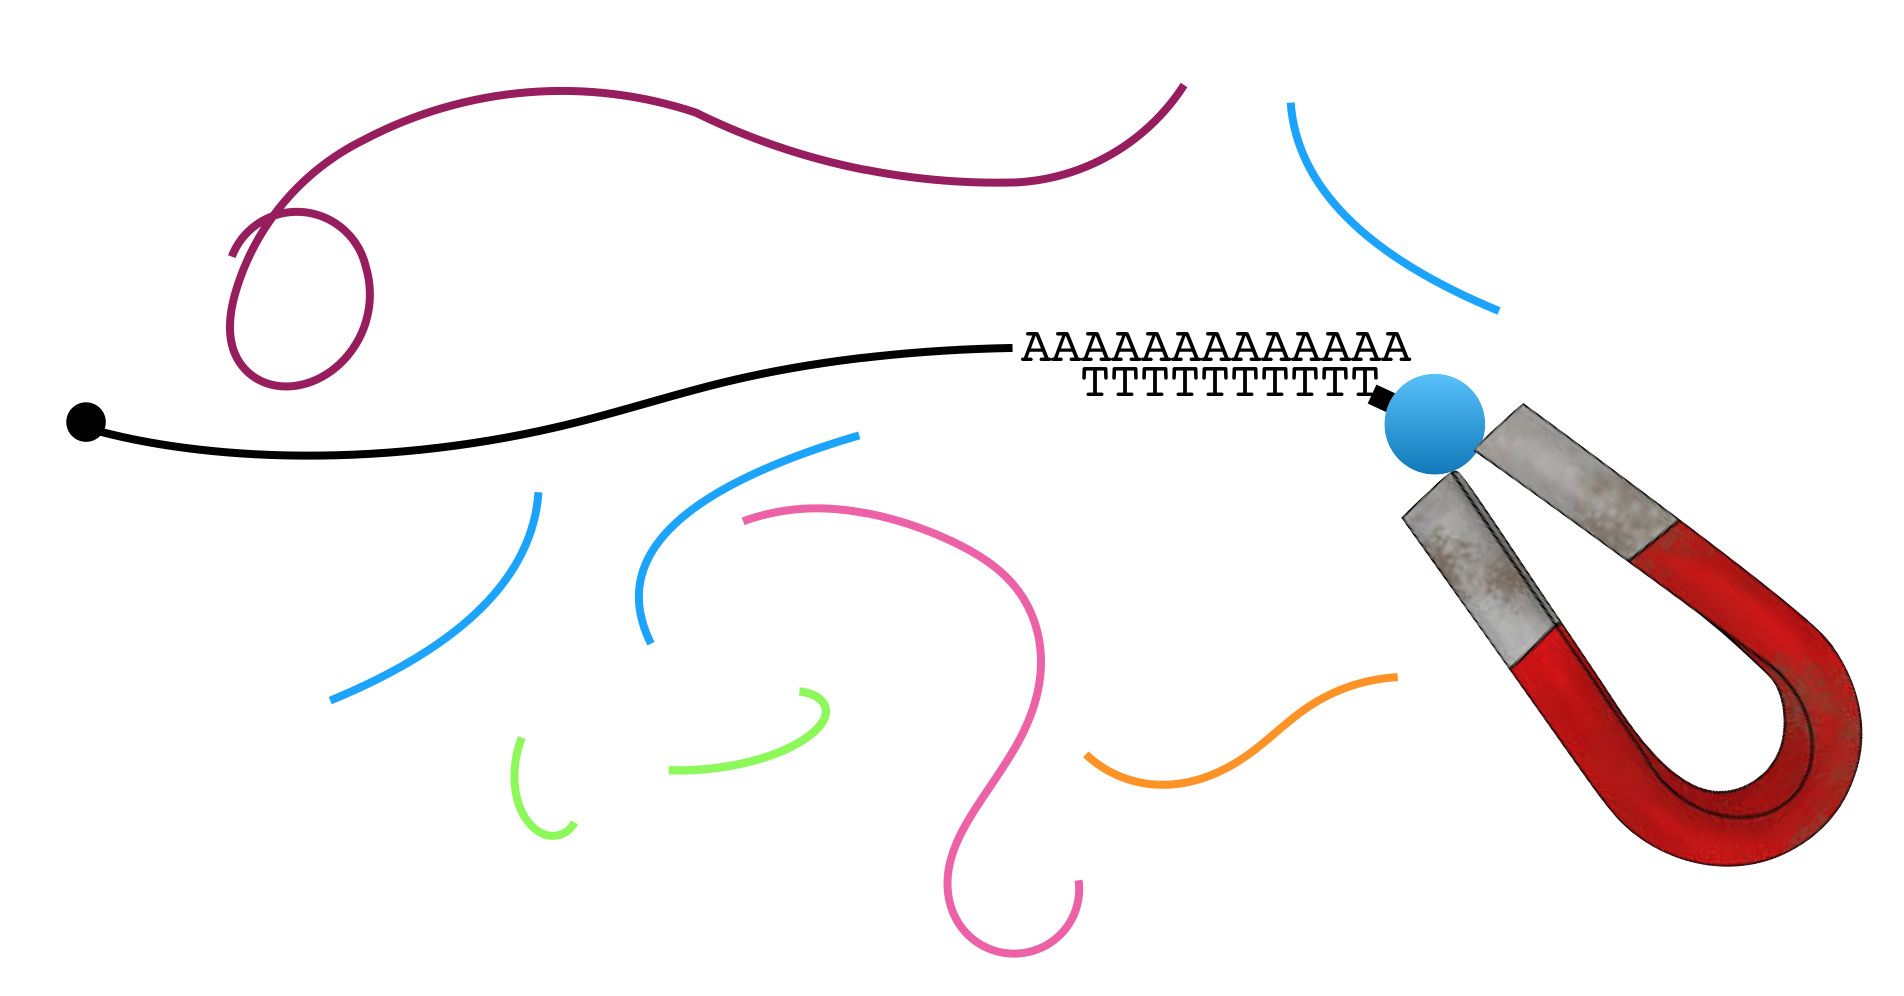
\includegraphics[width=1\linewidth]{static/images/mrnaextraction}

}

\caption{A common mRNA extraction method involves the use of magnetic beads attached to oligo dT. The oligo dT binds the poly A tail present on mRNA. The magnet captures the mRNA while the other types of RNA are removed during a washing step.}\label{fig:rnaextraction}
\end{figure}

The magnet holds on to the beads that are bound to mRNA (NOTE: Each bead actually has thousands of oligos attached and thus binds thousands of mRNA in the sample). All other RNAs can now be washed away. Then to separate the poly A+ mRNA from the oligo dT magnetic beads, gentle heat is applied. Once the mRNA has been collected, it can be broken into fragments in a variety of ways. In one methods, a light treatment with an enzyme called RNAse III is used. RNase III cleaves at random to break phosphodiester bonds in RNA chains.

Next the RNA fragments are converted into DNA. But how? Most DNA polymerases are so-called \emph{DNA-dependent, DNA polymerases} and by definition cannot use RNA as a template for DNA synthesis. Luckily, retroviruses encode a unique type of DNA polymerase known as reverse transcriptase, which is an \emph{RNA-dependent DNA polymerase}! Like most DNA polymerases, however, reverse transcriptase can only add new nucleotides to the 3' end of a pre-existing chain. Thus, a primer is needed. There are two options: 1) the use of so-called random primers \footnote{random primers are a mixture of oligonucleotides representing all possible sequence for a given size (i.e.~hexamers are common). Random Primers can be used to prime cDNA synthesis (modified from Bioline).} which will anneal at `random' along the fragmented RNA molecules to prime DNA synthesis or 2) the use of a sequence specific primer that has been designed to anneal to an RNA oligo that had been ligated to the 3' end of all the fragmented RNAs.
Whichever method is used to prime DNA synthesis, the resulting DNA produced is called complementary DNA or cDNA (it is complementary to the template RNA). The millions of unique cDNA molecules converted from RNA fragments are then sequenced using a high throughput sequencing method (i.e.~Illumina or Ion Torrent). All the millions of short ``sequence reads'' obtained are then computationally aligned (Figure \ref{fig:rnaseq}, \emph{in silico}\footnote{\textbf{\emph{in silico}} is an expression meaning ``performed on computer or via computer simulation'' in reference to biological experiments}) to a reference genome assembly. In Figure \ref{fig:alignmentread}, you can get a sense for what it means to align sequence reads to a reference genome\footnote{A reference genome (also known as a reference assembly) is a digital nucleic acid sequence database, assembled by scientists as a representative example of the set of genes in one idealized individual organism of a species (wikipedia definition).}. So long as a sequence read is long enough you can align it to a \emph{single} region of the genome with confidence.

\begin{figure}

{\centering 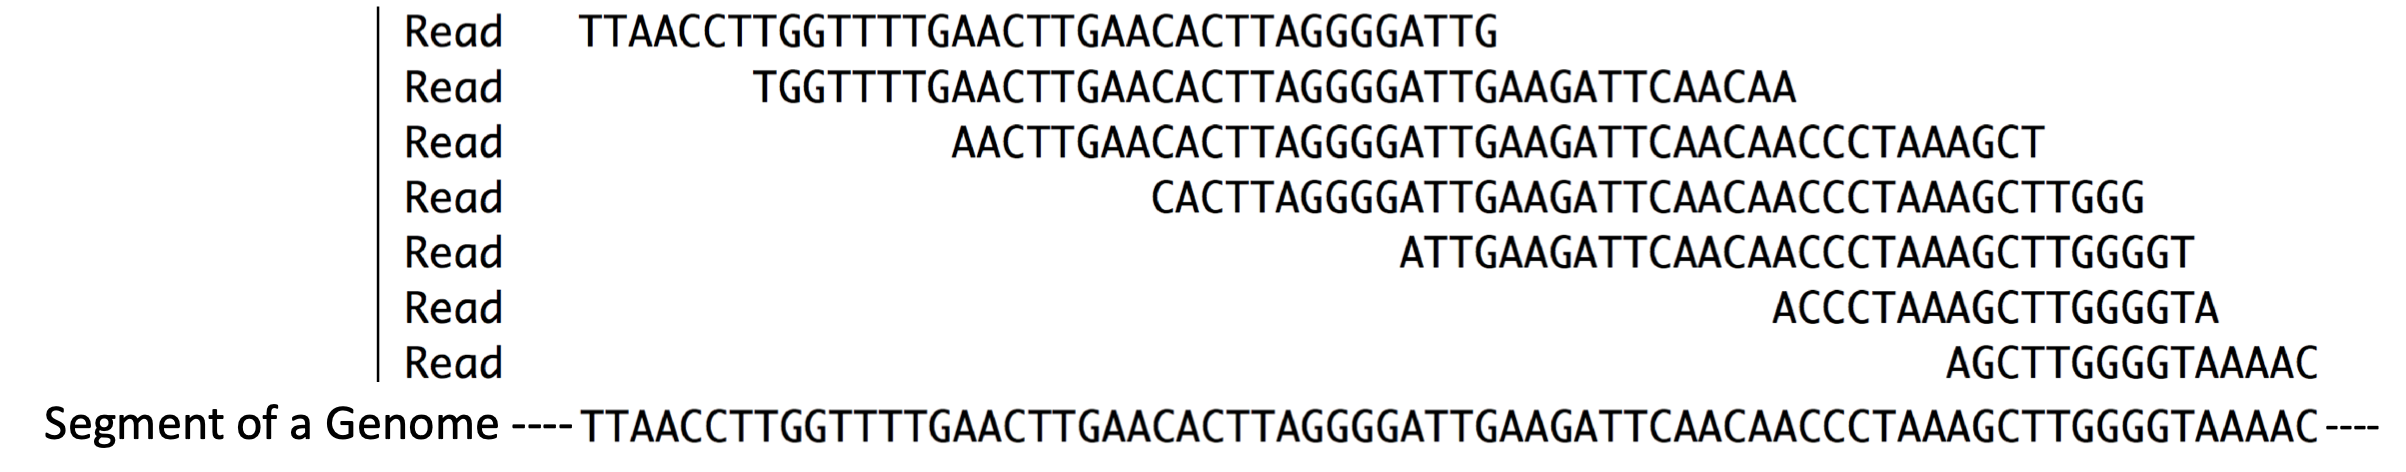
\includegraphics[width=1\linewidth]{static/images/readalignment}

}

\caption{Reads = Sequence reads. They are typically short. These sequence reads align (match) the short segment of genome shown below. Compare the sequences that are placed directly above one another.}\label{fig:alignmentread}
\end{figure}

In summary, RNAseq provides \emph{unbiased}, experimental evidence that a given segment of a genome is transcriptionally ``active'' and thus harbors a gene. Why do I say ``unbiased''? No prior knowledge about the gene sequence or location of the gene in the genome is necessary for a gene to be identified. Moreover, RNAseq can reveal \emph{how} transcriptionally active a gene is in a given RNA sample by keeping track of the \emph{number of reads} that map to a specific site in the genome. Genes that are highly transcribed are expected to produce on average more sequence reads than a gene that transcribed to lower levels. That said, the absence of sequence reads for a given segment of genomic DNA does NOT indicate the absence of a gene in that region of the genome. After all, muscle tissue is not expected to express the same set of genes as brain tissue. That said, more and more genes will be identified by RNA-seq as more and more RNA-seq experiments are performed using RNA extracted from different types of samples (and different environmental conditions).

\textbf{The take home messages}: RNAseq is a misnomer, RNA is \textbf{NOT} sequenced directly. Only DNA that is made using RNA as a template is sequenced!

\hypertarget{test-your-understanding-10}{%
\subsection{\texorpdfstring{\href{https://docs.google.com/forms/d/e/1FAIpQLSewKpJdsq0wm_uRGAblrKawwG5mvWVZieFe2sh1cH8FHjEpOg/viewform?usp=sf_link}{Test Your Understanding}}{Test Your Understanding}}\label{test-your-understanding-10}}

\begin{itemize}
\tightlist
\item
  \emph{RNA-sequencing involves the sequencing of which molecule (DNA, RNA or protein)?}
\item
  \textbf{True or False}: \emph{In order to purify mRNA for RNA-seq (not tRNA, rRNA etc) you can use magnetic beads covered in random primers.}
\item
  \textbf{True or False}: \emph{In order to purify mRNA for RNA-seq (not tRNA, rRNA etc) you can use magnetic beads covered in oligo dT primers.}
\item
  \emph{What type of polymerase is Reverse Transcriptase?}
\item
  \emph{What purpose does RNAse III serve in the RNA-sequencing method?}
\item
  \emph{In general, where can RNAseq reads map (given high levels of gene expression)?}
\end{itemize}

\hypertarget{understanding-the-encode-rna-seq-evidence-track}{%
\section{Understanding the Encode RNA-seq Evidence Track}\label{understanding-the-encode-rna-seq-evidence-track}}

The UCSC Genome Browser contains numerous evidence tracks containing RNA-seq data from a variety of labs and institutes. Again, these tracks are useful for visualizing regions of the genome that are transcriptionally active. We will focus on one evidence track entitled, ``Encode RNA-seq\ldots{}'' that maps RNA sequencing data from the ENCODE project. The overall goal of the ENCODE project is to identify and characterize transcribed regions of the human genome. I like this evidence track because it lets you see the alignment of individual sequence reads to the reference genome.

To load the Encode RNA-seq evidence track focused on BBS1, click on the \href{https://genome.ucsc.edu/s/megallegos/Biol\%20310\%3A\%20Module\%202\%20RNA\%2Dseq}{``RNA-seq'' session link}. Your evidence track display window will look like Figure @ref(fig:seqreads (excluding my annotations in red). Scroll down to the ``Expression'' category to see that the ``Encode RNA-seq\ldots{}'' evidence track is now set for ``show''. Also, notice we are viewing the 2009 Genome Assembly. This is because the ``Encode RNA-seq\ldots{}'' evidence track is only available for this genome assembly and not the newer 2013 genome assembly. Why? Evidence tracks are curated by real people (groups of scientists). When scientists change jobs or move to new projects they may not always be available to update an evidence track so that it can be used with more recent genome assemblies.

\begin{figure}

{\centering 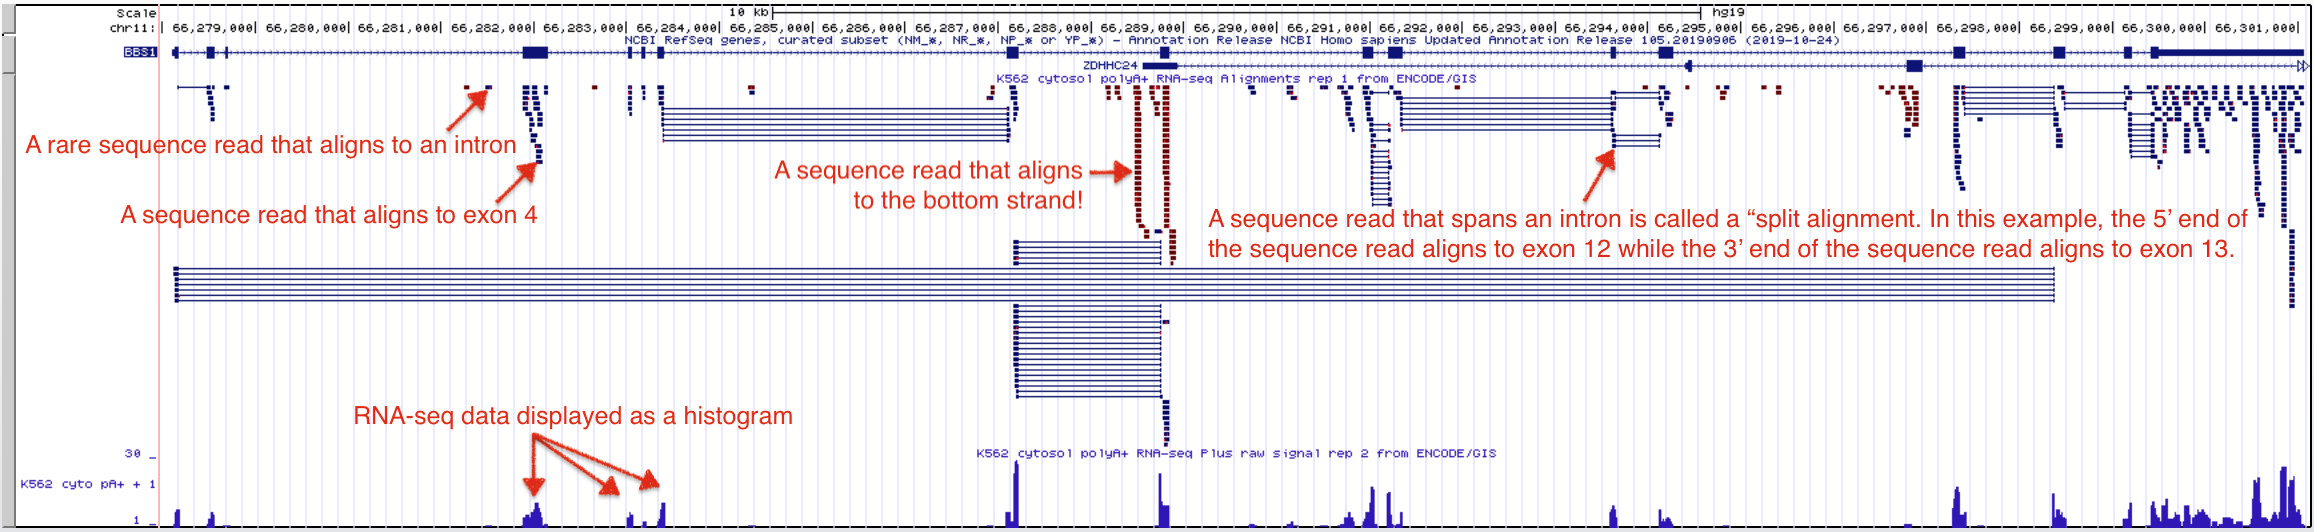
\includegraphics[width=1\linewidth]{static/images/sequencereads}

}

\caption{The Encode evidence track here shows high throughput sequencing of RNA samples from the K562 immortal cell line. The Alignment view on top shows where the sequence reads align to the genome including alignments that map to a single exon and *split alignments* that are interrupted by an intron. Sequences determined to be transcribed on the positive strand are shown in blue. Sequences determined to be transcribed on the negative strand are shown in red. Click on the image to enlarge.}\label{fig:seqreads}
\end{figure}

The RNA-seq data displayed in Figure \ref{fig:seqreads} corresponds to an RNAseq experiment performed at the Genome Institute of Singapore in 2009. In this experiment, RNA was extracted from K562 cells, an immortal cell line that was established in 1970 from fluid that built up around the lungs of a 53-year-old woman with chronic myelogenous leukemia. The extracted RNA was purified over a column containing oligo dT magnetic beads aimed at enriching for polyA+ RNA (mRNA) and removing contaminants (e.g.~rRNA, tRNA, DNA, protein etc.). The mRNA was then fragmented into small, random-sized pieces then converted into cDNA by reverse transcriptase. This cDNA library\footnote{\textbf{Library}: There are many types of libraries in molecular biology including cDNA and genomic libraries. A cDNA library is a complex mixture of cDNA representing all the genes that were transcriptionally active at the time of RNA collection. A genomic library is a complex mixture of genomic DNA fragments that in sum include all the genomic DNA for a given species. The DNA fragments are stored in DNA vectors such that each vector contains a unique insert of DNA.} were amplified by PCR\footnote{the Polymerase Chain Reaction or PCR is a powerful molecular technique designed to make multiple copies of any DNA sequence below a certain size} then sequenced. Short, 35 bp sequence reads were collected and computationally aligned to the genome assembly. How did I know all this? Right click on the gray rectangle at the far left of the Encode RNA-seq evidence track to view its ``Track Settings'' page. Scroll down to read the ``Methods'' then when you are done click on the K562 link to learn more about the cell line used in the study. The UCSC Genome Browser is rich with information worth exploring. If you ever get lost down a rabbit hole simply click the the \href{https://genome.ucsc.edu/s/megallegos/Biol\%20310\%3A\%20Module\%202\%20RNA\%2Dseq}{``RNA-seq'' session link} to get back to the beginning.

The RNA-seq data is displayed in the UCSC Genome Browser in two ways: as individual sequence read alignments and as a histogram. In the top half of the evidence track, the sequence read alignments are displayed in blue or red. The tiny blue horizontal lines represent reads that align and match the top strand (these sequence reads align to BBS1, a top strand gene), while the tiny, red lines represent sequence reads that align and match the bottom strand (these sequence reads align to the position of bottom strand genes). Notice that some sequence read alignments are interrupted by a very thin, horizontal line. These are called ``split alignments''.

Split alignment sequence reads are less intuitive. Recall that this RNA-seq experiement involved the sequencing of fragmented mRNA (not tRNA, rRNA, pre-mRNA etc.). Since mRNAs lack introns and the RNA fragmentation process is random, a single sequence reads can align to \textbf{two} adjacent exons in the genome. To indicate that a single sequence read aligns to two adjacent exons, they are connected by a thin line. These types of sequence reads are particularly useful because they provide information about the position of exon-intron junctions. Review Figure \ref{fig:splitalign} to view an example of a split alignment spanning a particularly short intron found in a gene called PLXNA3. In this figure I provide the actual sequence of a sequence read and a pairwise alignment to the genome. You can see this type of information for yourself by clicking on any individual sequence read. This action takes you to the sequence read information page.

\begin{figure}

{\centering 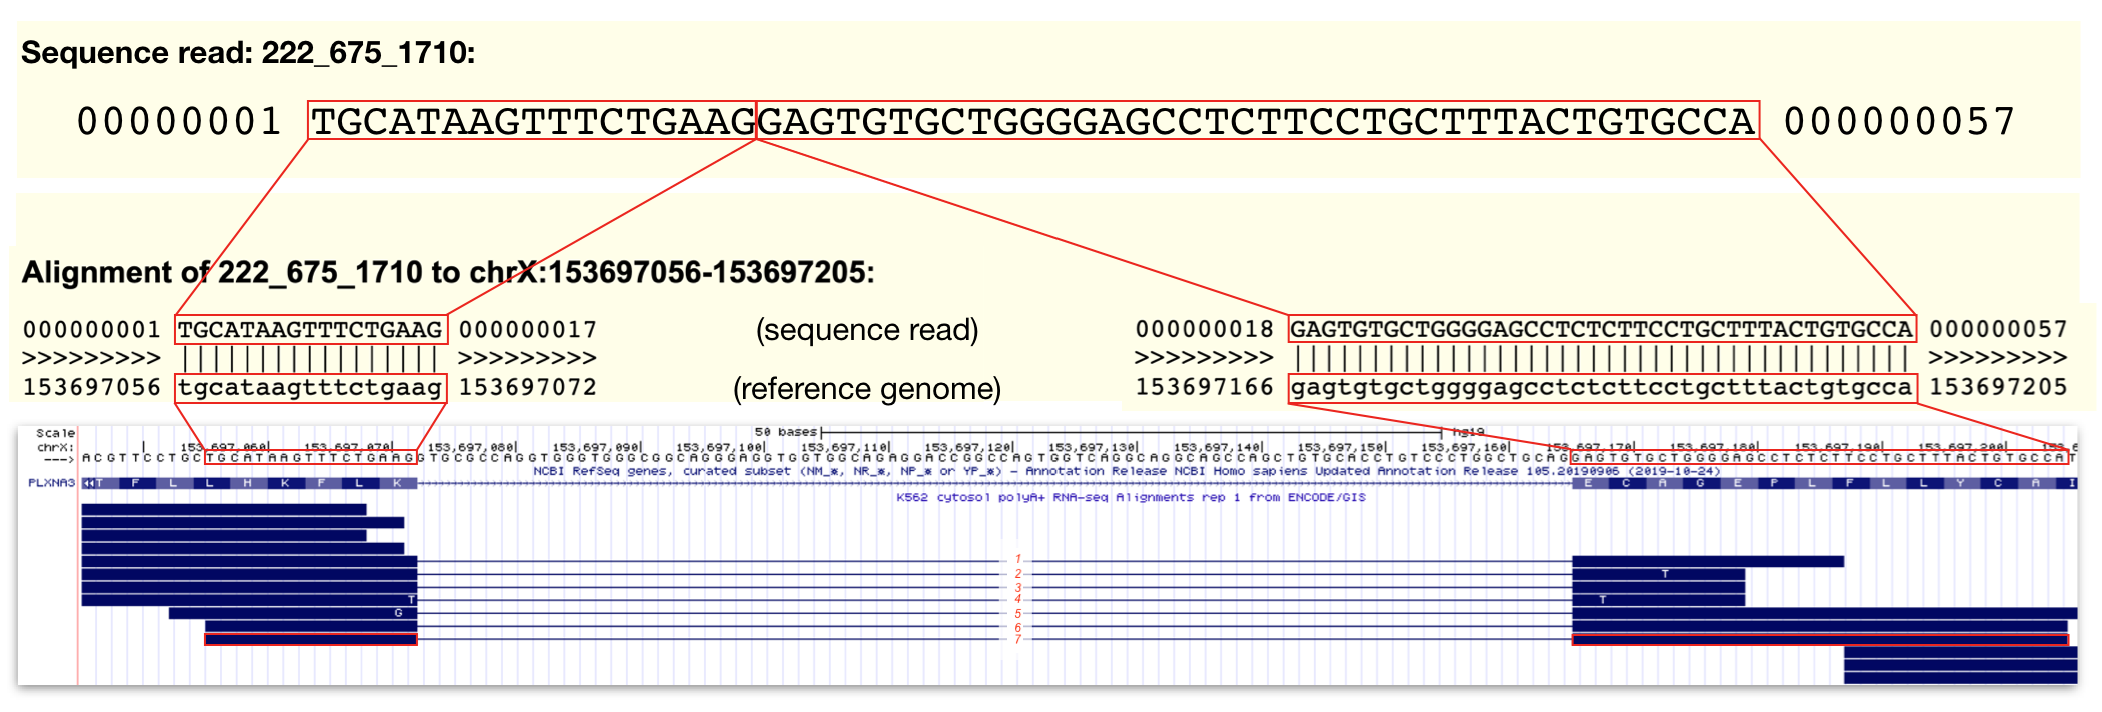
\includegraphics[width=1\linewidth]{static/images/splitalignment}

}

\caption{The top panel contains the sequence data for a single sequence read (read ID: 222_675_1710). The middle panel displays the alignment between this sequence read and the reference genome. Regions identical in sequence are boxed and connected by lines. Notice that the alignment is *split*. **This is because the sequence read does NOT align to one single contiguous stretch of genomic DNA**. The bottom panel is a display of all the sequence read alignments that map to a small region of PLXNA3 including 222_675_1710 outlined in red. In this region, I count 6 split alignments that span intron 24 of PLXNA3. Click image to enlarge.}\label{fig:splitalign}
\end{figure}

The bottom section of the Encode RNA-seq window shows the sequence read data as a \textbf{histogram} (Figure \ref{fig:seqreads}). As in all histograms, the Y-axis represents frequency (in this specific case, it represents the number of ``reads'' counted or ``read counts'') and the X-axis represents chromosomal position (in bp). In general, the histogram graphically describes how many sequence reads are found to align to a given nucleotide position in the genome. The taller the peak, the more ``reads'' that are counted for that particular nucleotide. You should know our evidence track is configured so that the histogram data for the bottom strand is hidden \emph{and} the maximum number of reads found in the window is shown on the Y axis. To better understand how to read the RNA-seq histogram data, zoom into exon 4 of BBS1. Your view should look like Figure \ref{fig:histogramannotated}. At this level of resolution, you can better count individual sequence reads. Notice the maximum number of reads in the Y-axis has changed to 11 (used to be 58). Also, notice that the number of reads for any given nucleotide position along exon four varies depending on the number of read counts for that nucleotide.

\begin{figure}

{\centering 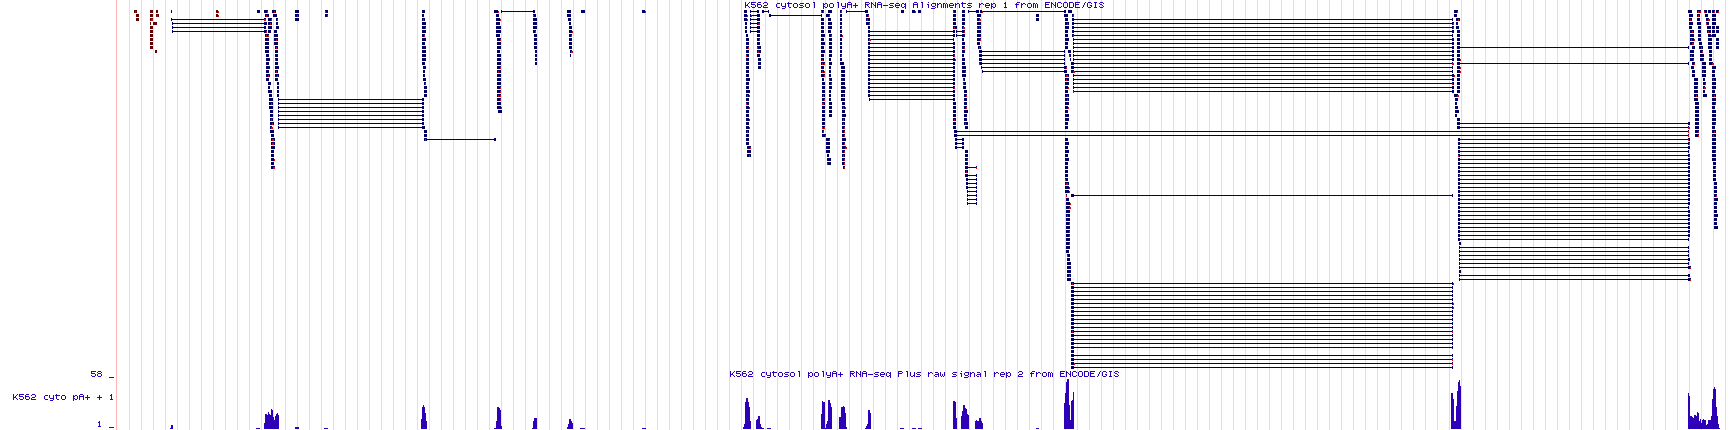
\includegraphics[width=1\linewidth]{static/images/histogram}

}

\caption{A close up view of exon 4 of BBS1. Notice the Y axis for the histogram indicates that the maximum number of sequence reads that map to this region is 11. The height for any given region of the histogram is determined by the number of reads counted. On the left, I highlight a region of exon 4 that has 5 total reads. On the right I highlight a region of exon 4 that has 2 total reads. Click image to enlarge.}\label{fig:histogramannotated}
\end{figure}

\hypertarget{test-your-understanding-11}{%
\subsection{\texorpdfstring{\href{https://docs.google.com/forms/d/e/1FAIpQLScSof7sO3S_09-Ulow0qixD-qie0n7pTp2NdDonfaV8waKO-A/viewform?usp=sf_link}{Test Your Understanding}}{Test Your Understanding}}\label{test-your-understanding-11}}

The following questions correspond to the RNAseq data collected from K562 cells -- start with the \href{https://genome.ucsc.edu/s/megallegos/Biol\%20310\%3A\%20Module\%202\%20RNA\%2Dseq}{``RNA-seq'' session link}. Submit your answers online but also write them down so that you can compare them to your answers in the next set of questions below.

\begin{itemize}
\tightlist
\item
  \emph{How many sequence reads map to exon 6 of BBS1}
\item
  \emph{How many split alignment reads connect exons 16 and 17 of BBS1?}
\item
  \emph{Search for the neighboring gene, ZDHHC24 (zoom out or search by name). Are there a significant number of sequence reads that align to ZDHHC24 (more than say 1-2)? NOTE: Before you answer, think about how you would recognize them given this is a negative strand gene.}
\item
  \emph{Search for the neighboring gene, ACTN3 (zoom out or search by name). Are there a significant number of sequence reads that align to ACTN3 (more than say 1-2)?}
\end{itemize}

You have been evaluating RNAseq data collected from K562 cells. Let's look at a different RNAseq experiment. \textbf{To switch data sets}, click on the gray rectangle (at left) corresponding to the ``Encode RNA-seq'' evidence track to view the track settings page. Within track settings, unclick the K562 data set and click on the \textbf{H1-hESC} data set. To see what type of cells these are, click on the ``H1-hESC'' link. Copy (control C) the information in the description column. Now hit ``Submit'' to go back to the browser display window.

\hypertarget{test-your-understanding-12}{%
\subsection{\texorpdfstring{\href{https://docs.google.com/forms/d/e/1FAIpQLSf4fcc57bfhUFKRBDyqeUTgSEvr4B9TKqiK8-EKO1P3AWJAgA/viewform?usp=sf_link}{Test Your Understanding}}{Test Your Understanding}}\label{test-your-understanding-12}}

The following questions are about the RNAseq data collected from H1-hESC cells. Submit your answers online but also write them down and compare these answers to the ones you completed above.

\begin{itemize}
\tightlist
\item
  \emph{What kind of cells are h1-hESC (Copy and paste your answer from the web to avoid typos)?}
\item
  \emph{How many sequence reads map to exon 6 of BBS1}
\item
  \emph{How many split alignment reads connect exons 16 and 17 of BBS1?}
\item
  \emph{Zoom out 10X to find the downstream gene, ZDHHC24. Are there any sequence reads aligning to ZDHHC24?}
\item
  \emph{Find another downstream gene, ACTN3. Are there any sequence reads aligning to ACTN3?}
\item
  \emph{How does the RNAseq data compare between the two cell types (K562 cells vs h1-hESC)?}
\end{itemize}

\hypertarget{for-discussion-1}{%
\subsection{\texorpdfstring{\href{https://docs.google.com/forms/d/e/1FAIpQLSfvvzUFBLKvVkvlxCiw_rfX5ykAsYTjVueqoJR14zbL4wplJg/viewform?usp=sf_link}{For Discussion}}{For Discussion}}\label{for-discussion-1}}

\begin{enumerate}
\def\labelenumi{\arabic{enumi}.}
\tightlist
\item
  When BBS1 is transcribed, full length mRNA molecules are produced (from exon 1 to 17). And so one might expect that the number of sequence reads that map to different parts of the gene would be produced at a more or less equal number. They are not. For example, compare the number of sequence reads that align to exon 5 to the number of sequence reads that align to exon 6. Alternatively, compare the number of \emph{split alignments} that link exons 1 to 2 to the number of split alignments that link exons 11 to 12. Why do you think the number of sequence reads and/or split alignments varies along the length of a single gene?
\item
  What about differences between data sets? Why do you think there was such a profound difference between the RNA-seq data collected from H1-hESC cells compared to K562 cells?
\item
  Finally, compare the exon-intron junctions in the gene prediction track (NCBI Refseq genes) to all the split alignments found experimentally (by RNA sequencing of K562 cells or H1-esc). There is at least one \emph{unexpected} split alignment read in BBS1 that suggests that there may be an alternative splice form not predicted by the NCBI Refseq gene prediction track. Do you see the same \emph{unexpected} split alignment read in the H1-ESC data set? Describe the alternative splice form as precise as possible. Do you think this alternatively splice form is real or an artifact of the RNA-seq method? Look at each unexpected split alignment read sequence before you answer.
\end{enumerate}

\hypertarget{take-home-messages}{%
\section{Take Home Messages}\label{take-home-messages}}

\begin{itemize}
\tightlist
\item
  RNA-seq data shows which parts of the genome are transcriptionally active (and how active!).
\item
  Because mostly mRNA is ``sequenced'' (at least that is the goal), RNA-seq reads mostly map to exonic regions (only pre-mRNA has introns).
\item
  Due to gene density in some parts of the genome and because mammlian introns can be long, RNA-seq data alone is not always able to define where a transcript begins and ends.\\
\end{itemize}

© 2019, Maria Gallegos. All rights reserved.

\hypertarget{gene-discovery-with-tss-seq}{%
\chapter{\texorpdfstring{\emph{Gene Discovery with TSS-seq}}{Gene Discovery with TSS-seq}}\label{gene-discovery-with-tss-seq}}

TSS stands for Transcriptional Start Site, also known as the +1 position of transcription\footnote{The +1 position marks the position of the first \emph{templated} nucleotide of the transcript. You may already know that a 5' cap is added to the mRNA. As a result, the +1 position of transcription becomes the second nucleotide of the mRNA.}. In this module, you will learn how RNA sequencing near transcriptional start sites (TSS-seq) is done, how the sequence data is displayed in the UCSC Genome Browser and how this data can be used to surmise where the \emph{beginning} of genes are located in the genome. You will also see how TSS-seq together with RNA-seq (Chapter 4) provides a more complete picture of where individual genes are located. To follow along with the text and to answer ``Test Your Understanding'' questions, begin with the \href{https://genome.ucsc.edu/s/megallegos/Biol\%20310\%3A\%20Module\%202\%20TSS\%2Dseq}{``TSS-seq''} session at the UCSC Genome Browser.

\hypertarget{how-tss-seq-is-done.}{%
\section{How TSS-seq is done.}\label{how-tss-seq-is-done.}}

How might one identify the transcriptional start sites of most genes in the genome without prior knowledge of where those start sites are located? Recall that mRNA has \emph{two} unique features: 1) a 5' cap and 2) a 3' poly A tail. While both can be exploited to purify mRNA away from all other RNA types, the 5' cap can be used specifically to pinpoint the transcriptional start site (TSS) as it is only added to the \emph{beginning} of a message (mRNA) By sequencing only that portion of the mRNA that is next to the 5' cap you can identify the TSS! Dubbed TSS-seq, these sequence reads are then aligned to a reference genome as is done for RNA-seq.

The steps necessary to prepare mRNA for TSS-seq are outlined in Figure \ref{fig:TSSseqsteps}. First, poly-A containing RNA (mRNA) is extracted from an organism, tissue or cell of interest as described previously (Figure \ref{fig:rnaextraction}). Due to the fragility of RNA in general, RNA extractions typically include full length mRNA (with a 5' cap) and partially degraded mRNA (with a 5' phosphate instead). You do not want to sequence the 5' ends of partially degraded mRNA as these molecules do not pinpoint the location of the TSS but instead map to the interior of a gene.

\begin{figure}

{\centering 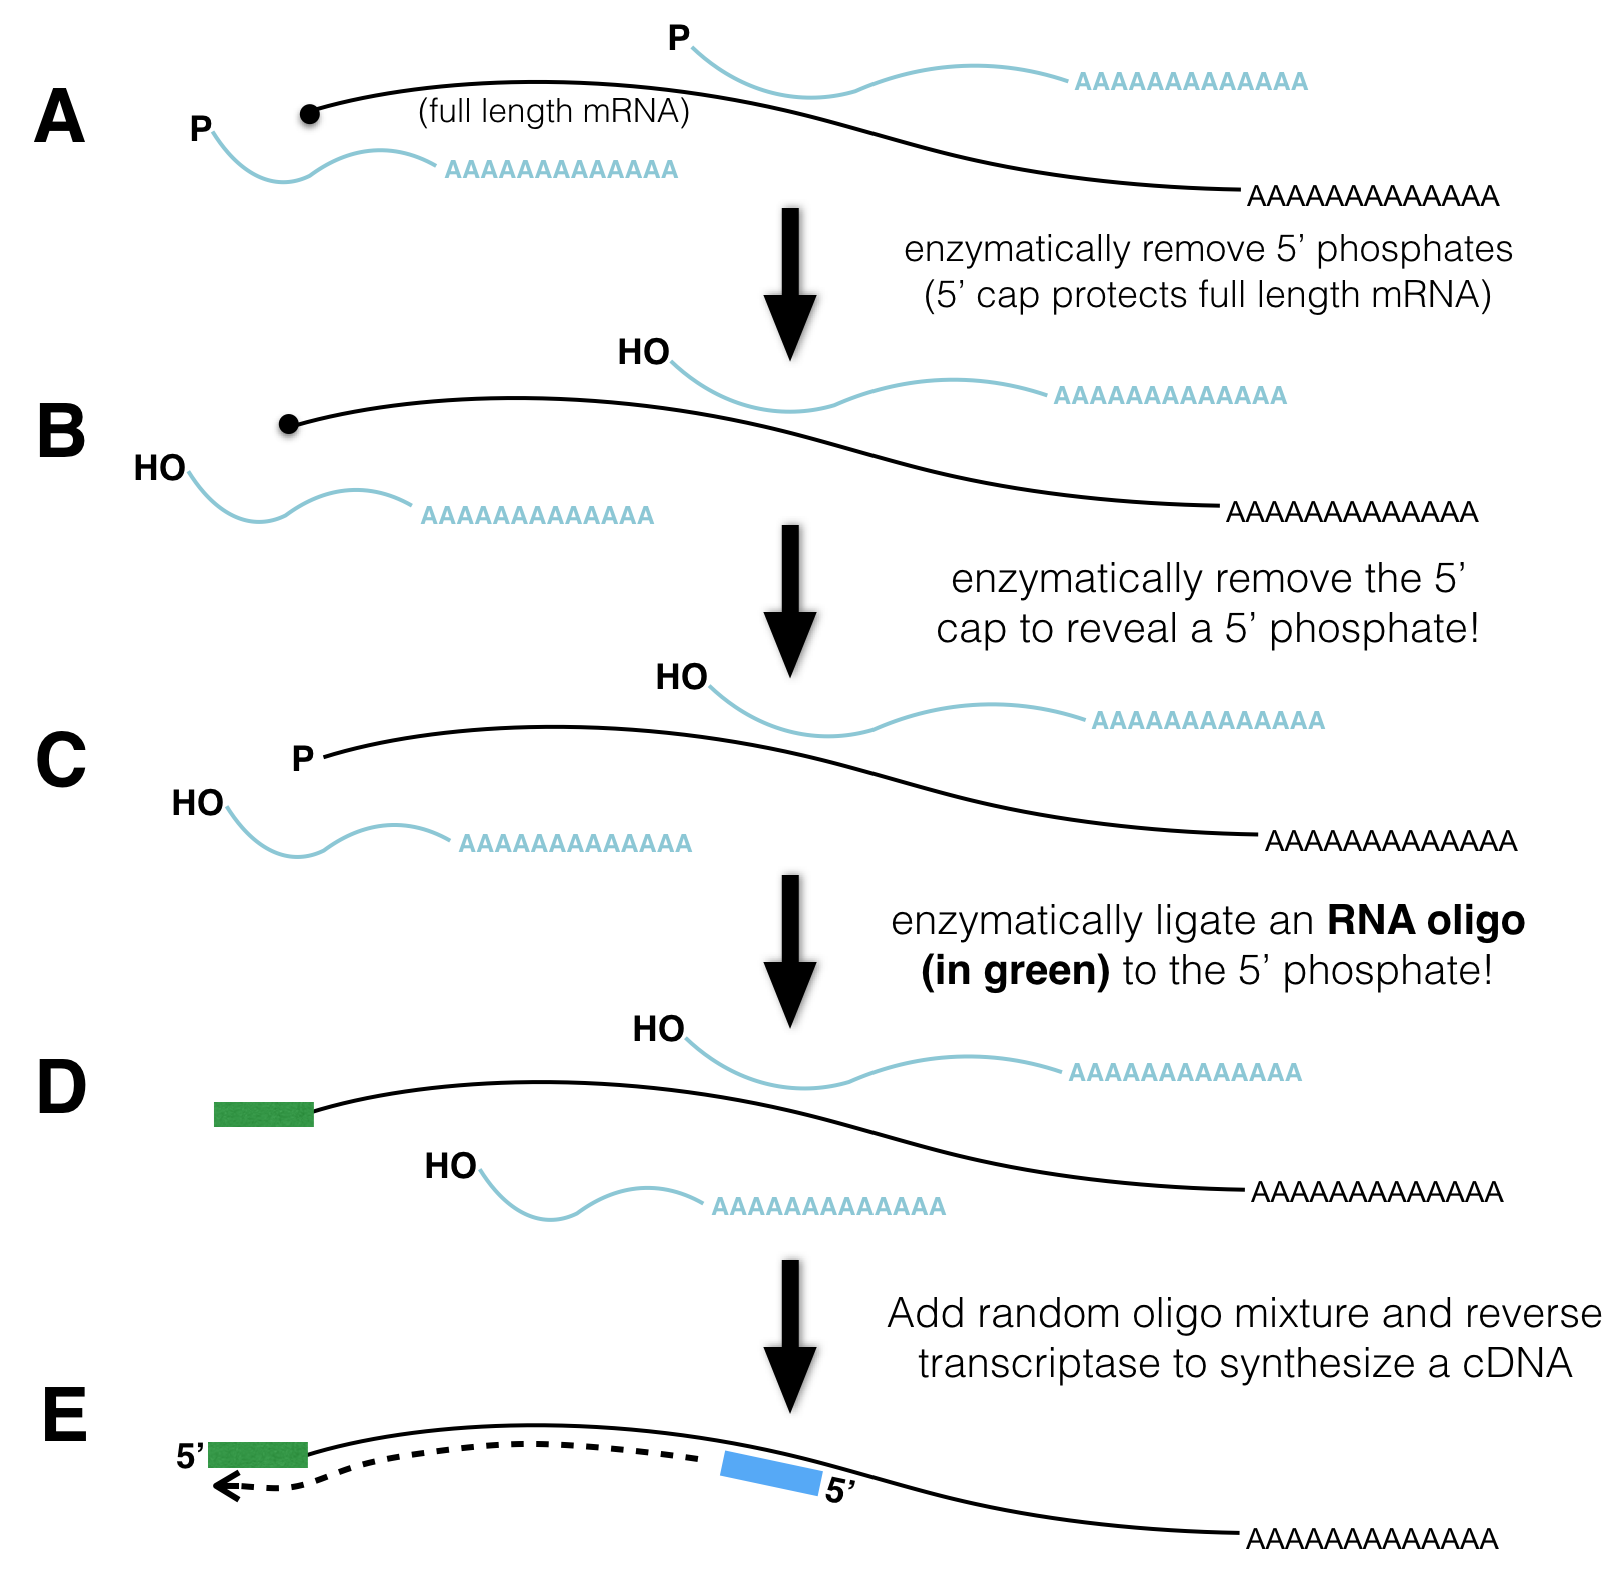
\includegraphics[width=0.75\linewidth]{static/images/TSSseqmethod}

}

\caption{TSSseq protocol. A) All mRNA possessing a poly A tail is separted from total RNA. The resulting sample contains both full length mRNA with a 5' cap and partially degraded mRNA with a 5' phosphate (P-). B) An enzyme that removes 5' phosphates is added. See the P change to OH. C) An enzyme is added that removes the 5' cap structure. See the black circle change to a P. D) RNA ligase attaches an RNA oligo (green rectangle) to all RNAs that had a 5' phosphate in C). E) The addition of reverse transcriptase and random oligos produce cDNA fragments. Those cDNA fragments that once had a 5' cap all have the same sequence at their 3' ends.}\label{fig:TSSseqsteps}
\end{figure}

How can one distinguish full length mRNA from partially degraded fragments? Scientists have devised a clever method: First, they add an enzyme that removes 5' phosphates from \emph{all} partially degraded RNA molecules in the tube. Full-length, capped mRNAs do not possess a 5' phosphate and are thus impervious to\footnote{not affected by} this step. Next, they add an enzyme that removes the 5' cap from full length mRNAs. Now the full-length mRNAs that were once capped possess a 5' phosphate instead\footnote{At this point, full length mRNA possess a 5' phosphate while partially degraded mRNA posses a 5' hydroxyl - so they are still different and distringuishable}! Next, RNA ligase\footnote{\textbf{RNA ligase} is similar to DNA ligase in that both require a 5' phosphate and a 3' hydroxyl to form a phosphodiester bond between two nucleic acid chains. The main difference: RNA ligase links two RNA chains together while DNA ligase links two DNA chains together} is used to attach a single-stranded \textbf{RNA} oligo\footnote{Short single-stranded RNA chain} to the 5' end of only those RNAs that have 5' phosphates. Finally, \emph{all} the RNA in the tube is converted into cDNA using a reverse transcriptase and random primer (as described previously). Importantly, only those cDNAs that once had a 5' cap are tagged with the specific primer sequence at their 3' end (NOTE: Do you understand why this primer sequence is now at the 3' end of the DNA?). This 3' sequence tag can now be exploited for sequencing as the sequencing reaction is primed with a DNA oligo that base pairs\footnote{The phrase ``base pairs'' here is used as a verb to mean ``hybridizes to'' or ``anneals to''} to the sequence tag. The short sequence reads that are collected (about 35 bp in length) are then computationally aligned to the genome and counted as described previously (chapter 4).

\hypertarget{why-tss-seq-is-useful}{%
\section{Why TSS-seq is useful}\label{why-tss-seq-is-useful}}

As we just saw, RNA-Seq data can identify segments of the genome that are transcribed \emph{and} remain in mRNA (introns are transcribed but removed from mRNA). In other words, this type of data is excellent for identifying the position of \textbf{exons}. Often, RNA-seq data will also reveal how exons are linked together (with split alignments). That said, it is not always sufficient for gene identification purposes. To identify an individual transcription unit (a single gene) with more confidence, it is better to know the position of the exons \emph{and} the TSS. To see this for yourself, review RNAseq data corresponding to a small region of the genome (Figure \ref{fig:RNAseqdataonly}). The NCBI Refseq gene prediction track is hidden on purpose. As you can see, the histogram and sequence read alignments including the split alignments are displayed. How many genes do you think are in this region? What is your rationale?

\begin{figure}

{\centering 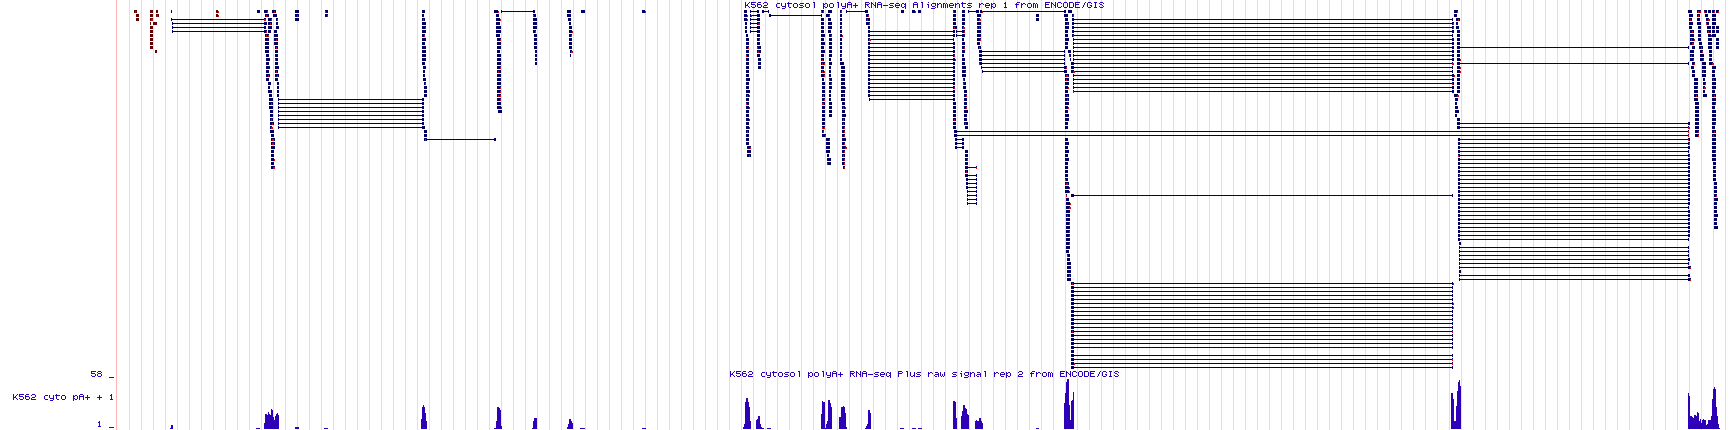
\includegraphics[width=1\linewidth]{static/images/histogram}

}

\caption{RNAseq data corresponding to a small region in the genome with the base position and gene prediction tracks hidden. Guess how many genes you think map to this region of the human genome.}\label{fig:RNAseqdataonly}
\end{figure}

In Figure \ref{fig:RNAseqdataonly}, there are two main groups of split alignments. It would be reasonable to guess that there are two genes in this region. To see the true number of genes click \href{https://genome.ucsc.edu/s/megallegos/DPP3}{here}. This link takes you to the same genome region as in Figure \ref{fig:RNAseqdataonly} but with the gene prediction and base position tracks visible. If you guessed wrong, do you see why you were misled?

\hypertarget{understanding-the-tss-seq-evidence-track}{%
\section{Understanding the TSS-seq Evidence Track}\label{understanding-the-tss-seq-evidence-track}}

The UCSC Genome Browser contains numerous evidence tracks displaying TSS-seq data. We will focus on one that was generated by the FANTOM5 Consortium of labs in Japan (FANTOM stands for Functional Annotation of the Mammalian Genome). Click the link to learn more about \href{http://fantom.gsc.riken.jp/}{FANTOM5}. FANTOM5 is a custom evidence track that I added by clicking on ``Add Custom Tracks'' then searching for ``FANTOM5''. To view this evidence track click the link for the \href{https://genome.ucsc.edu/s/megallegos/Biol\%20310\%3A\%20Module\%202\%20TSS\%2Dseq}{TSS-seq} session. You can also use this link as a starting point for questions related to TSS-seq data for any gene.

Your genome browser should now display the ``Max Counts of CAGE\footnote{CAGE is short for ''\textbf{C}ap \textbf{A}nalysis \textbf{G}ene \textbf{E}xpression''} reads'' evidence track for BBS1. This evidence track displays TSS-seq data in histogram form only (Figure \ref{fig:TSSseqforBBS1}). The track settings are configured such that that the Y-axis is set at 350 read counts. This can be changed at the track settings page for this evidence track. Setting the Y-axis at 350 is sufficient for most genes. For some highly expressed genes it is better to set the Y-axis to ````. Go to the track settings page. Scan down until you see''Data view scaling:``. Change the pulldown menu from''use vertical viewing range setting'' to ``autoscale to data view''. Then click submit. If you do this for BBS1, the Y-axis should end at 69.0667. Before you move on, change the Y-axis back to ``use vertical viewing range setting''.

\begin{figure}

{\centering 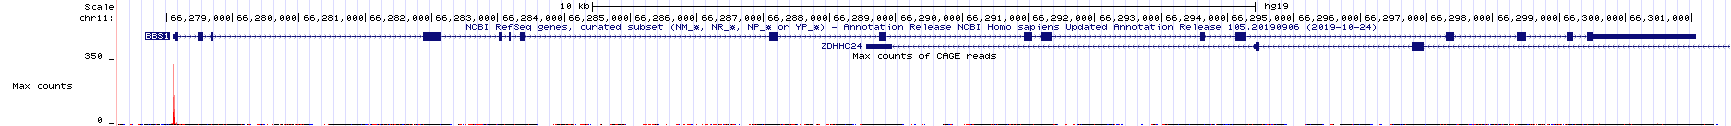
\includegraphics[width=1\linewidth]{static/images/TSSseqBBS1}

}

\caption{TSSseq data for BBS1.}\label{fig:TSSseqforBBS1}
\end{figure}

Zoom out 10X. The genome browser window is now focused on a larger portion of the genome surrounding BBS1 (Figure \ref{fig:TSSseqfor10X}). Notice that there are both red peaks and blue peaks. There are also tall peaks and tiny peaks.

Recall that genes can be found on the top strand or the bottom strand as RNA polymerase can use either strand as template for transcription. If RNA polymerase uses the bottom strand as template then it moves from left to right (5' to 3') and produces an mRNA that \emph{matches} the top strand sequence and is complementary to the bottom strand. If RNA polymerase uses the top strand as template then it moves from right to left (also 5' to 3' relative to the bottom strand) and produces an mRNA that matches the \emph{bottom strand} sequence. Histrogram peaks displayed in \textbf{red} represent the TSS of top strand genes. Histogram peaks displayed in \textbf{blue} represent the TSS of bottom strand genes.

The taller a histrogram peak at a given location, the more sequence reads that map to that region. The more read counts, the more reliable the data and the more likely the data represents a true TSS. In fact, the tiny peaks observed in Figure \ref{fig:TSSseqfor10X} (find each red asterix) likely reflect background noise\footnote{Molecular biology is messy. Each enzymatic step listed in Figure \ref{fig:TSSseqsteps} is not likely to achieve 100\% success. For example, partial mRNAs that fail to have their 5' phosphates removed can be sequenced along side all the true full-length mRNAs.} and may not represent the position of a TSS at all. That said, the \emph{absence} of a peak at a location where one was predicted to exist does not mean that the gene prediction is incorrect. This might be an instance where a gene was not expressed in the tissue sample that was used to generate the TSS-seq data. There is a common saying, ``Absence of evidence is not evidence of absence''.

\begin{figure}

{\centering 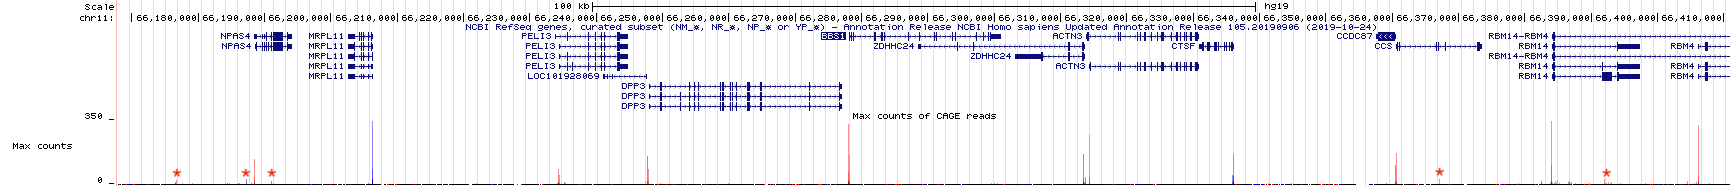
\includegraphics[width=1\linewidth]{static/images/TSSseq10X}

}

\caption{TSSseq data of a larger region surrounding BBS1. Each asterix (my annotation) highlights sequence reads that are not likely to represent true transcriptional start sites.}\label{fig:TSSseqfor10X}
\end{figure}

Now zoom in to the TSS for BBS1 (Figure \ref{fig:TSSclose}). You can see that the majority of experimentally defined TSSs are located at the predicted transcriptional start site. This is not always the case. Also, notice that there are a range of TSSs for BBS1. This is normal.

\begin{figure}

{\centering 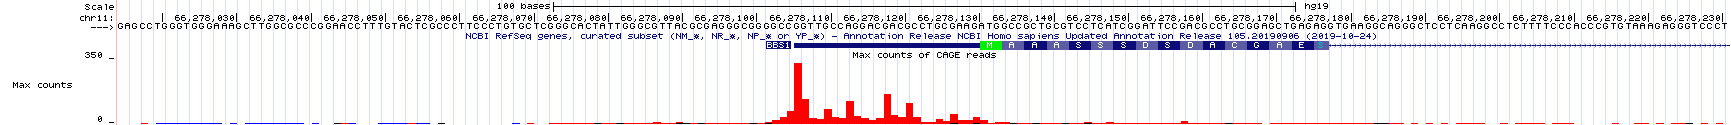
\includegraphics[width=1\linewidth]{static/images/TSSBBS1close}

}

\caption{A close up view of the TSS-seq histogram data surrounding the predicted **transcriptional** start site for BBS1 (as defined by the NCBI refseq evidence track). The **translational** start site of BBS1 is shown in green.}\label{fig:TSSclose}
\end{figure}

If you zoom in even farther you can determine the \emph{exact} nucleotide position of the TSS used most often in BBS1. \textbf{The first templated ribonucleotide of BBS1 is the ``G'' at position 66,278,106 on chromosome 11} (Figure \ref{fig:TSScloser}). To see how the nucleotide position is aligned to the nucleotide and the TSS-seq histogram data in the UCSC genome browser window, see the same image but annotated (Figure \ref{fig:TSScloserwithannotation}).

\begin{figure}

{\centering 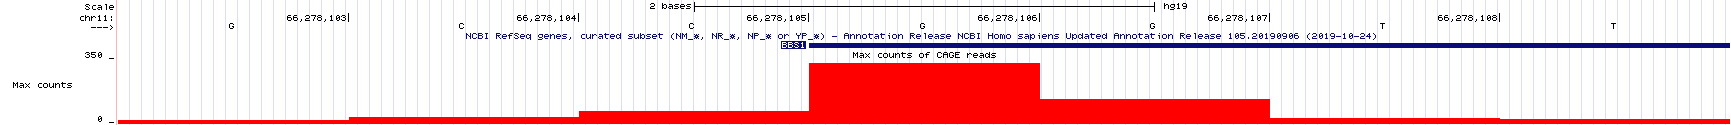
\includegraphics[width=1\linewidth]{static/images/TSSBBS1closer}

}

\caption{An even closer view of the TSS-seq histogram data surrounding the predicted transcriptional start site for BBS1. At this zoom level, the genome sequence *and* individual nucleotide positions are notable}\label{fig:TSScloser}
\end{figure}

\begin{figure}

{\centering 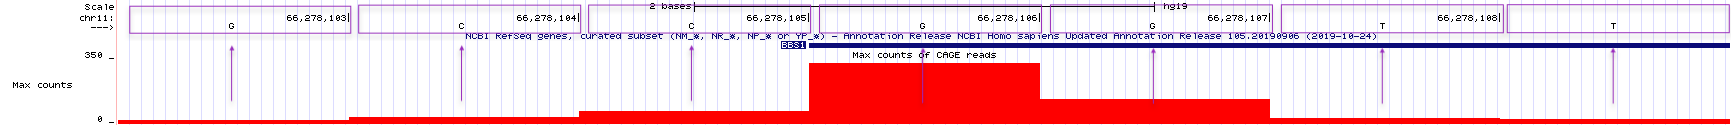
\includegraphics[width=1\linewidth]{static/images/TSSBBS1closerannotated}

}

\caption{An annotated version of the same view of BBS1 as above.}\label{fig:TSScloserwithannotation}
\end{figure}

Again, this is a great example of an evidence track that provides unbiased experimental evidence for the existence of a gene. It provides the position of all transcriptional start sites (TSS) within the genome. Each TSS identified by TSS-seq was not predicted to exist but was experimentally determined without prior knowledge (no bias).

That said, TSSseq data is not sufficient to determine the number of individual genes in a given region of the genome. For example, review the histrogram data in (Figure \ref{fig:TSSdataalone}) and try to predict the number of genes in this region. Again, I have omitted the gene prediction track. Moreover, there are individual genes that utilize alternative transcription initiation sites (Review chapter 3, ``One gene, many splice variants'')!

\begin{figure}

{\centering 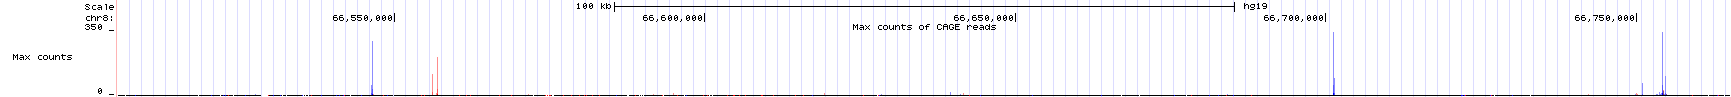
\includegraphics[width=1\linewidth]{static/images/TSSdataonly}

}

\caption{This is an image of the TSSseq evidence track for a small region of the human genome. All other tracks have been hidden. Count the number of transcription starts sites then guess how many genes you think these TSS peaks correspond to.}\label{fig:TSSdataalone}
\end{figure}

Only when a sufficient amount of RNAseq data \textbf{combined with} TSSseq data is available can one determine the number of genes in a given genomic region with confidence. Click \href{https://genome.ucsc.edu/s/megallegos/TSSproblem2}{here} to review the gene prediction track and RNAseq data for the genomic region shown in Figure \ref{fig:TSSdataalone} to see how the RNAseq data combined with the TSS seq data provides a more complete picture of the true number of genes present. How does this differ from what you thought? Do you see why you were misled?

\hypertarget{test-your-understanding-13}{%
\subsection{\texorpdfstring{\href{https://docs.google.com/forms/d/e/1FAIpQLSdoZhdWlHjqL4CDLwYROE0EiyIVDlYp0qbOYrwDt0HGiG7Dcg/viewform?usp=sf_link}{Test Your Understanding}}{Test Your Understanding}}\label{test-your-understanding-13}}

\textbf{The first three questions require the TSS-seq data displayed in the figure below.}

\begin{center}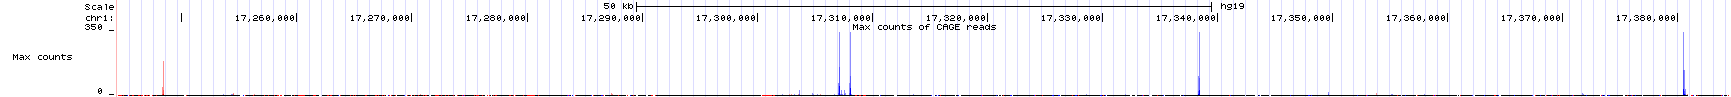
\includegraphics[width=1\linewidth]{static/images/TSSdataonlyTYU} \end{center}

\begin{itemize}
\tightlist
\item
  \emph{How many prominent transcription start sites (\textgreater50 Max Count Reads) can be found in the genome region displayed above?}
\item
  \emph{Among the TSS peaks displayed in the figure above, how many use the top strand as a template for transcription?}
\item
  \emph{Among the TSS peaks displayed in the figure above, how many involve RNA polymerase traveling from left to right?}
\end{itemize}

\textbf{Search for a gene called, DPF2. Then zoom into the region where transcription initiation occurs MOST prominently}.

\begin{itemize}
\tightlist
\item
  \emph{Where is this experimentally defined TSS peak relative to the predicted TSS for DPF2? To find the experimentally defined TSS, look at the TSS-seq data. By predicted TSS, look at the NCBI Refseq gene prediction track\footnote{NOTE: The UCSC gene prediction track may also open. This is a bug. If the added clutter is distracting, right click on its corresponding gray rectangle and choose ``hide''.}.}
\item
  \emph{Now determine the exact nucleotide position where transcription initiation occurs most often for DPF2 (enter a specific number).}
\item
  \emph{Now determine the first templated nucleotide (G A U or C) for DPF2. Choose the one that is observed most often.}
\end{itemize}

\hypertarget{test-your-understanding-14}{%
\subsection{\texorpdfstring{\href{https://docs.google.com/forms/d/e/1FAIpQLSewgrAT0bWLa87TPlI-dcFIbXBKRn0yrZw9ELWU6JgWWg9V_g/viewform?usp=sf_link}{Test Your Understanding}}{Test Your Understanding}}\label{test-your-understanding-14}}

\textbf{Search for a gene called, ANO9 then zoom into the region where transcription initiation occurs MOST prominently}.

\begin{itemize}
\tightlist
\item
  \emph{Where is this experimentally defined TSS peak relative to the predicted TSS for ANO9? To find the experimentally defined TSS, look at the TSS-seq data. By predicted TSS, look at the NCBI Refseq gene prediction track\footnote{NOTE: The UCSC gene prediction track may also open. This is a bug. If the added clutter is distracting, right click on its corresponding gray rectangle and choose ``hide''.}.}
\item
  \emph{Now determine the exact nucleotide position where transcription initiation occurs most often for ANO9 (enter a specific number).}
\item
  \emph{Now determine the templated nucleotide (G A U or C) for ANO9 that occurs most often.}
\end{itemize}

\textbf{Search for a gene called, ZDHHC24 then zoom into the region where transcription initiation occurs MOST prominently}

\begin{itemize}
\tightlist
\item
  \emph{Where is this experimentally defined TSS peak relative to the predicted TSS for ZDHHC24? To find the experimentally defined TSS, look at the TSS-seq data. By predicted TSS, look at the NCBI Refseq gene prediction track\footnote{NOTE: The UCSC gene prediction track may also open. This is a bug. If the added clutter is distracting, right click on its corresponding gray rectangle and choose ``hide''.}.}
\item
  \emph{Now determine the exact nucleotide position where transcription initiation occurs most often for ZDHHC24 (enter a specific number).}
\item
  \emph{Now determine the templated nucleotide (G A U or C) for ZDHHC24 that occurs most often.}
\end{itemize}

\hypertarget{for-discussion-2}{%
\subsection{\texorpdfstring{\href{https://docs.google.com/forms/d/e/1FAIpQLSeR06s09E1L8aZKmYzKyJwuSNjVxeYzn7mpXPM555K0qOM9Xw/viewform?usp=sf_link}{For Discussion}}{For Discussion}}\label{for-discussion-2}}

\begin{enumerate}
\def\labelenumi{\arabic{enumi}.}
\tightlist
\item
  What surprised you the most as you reviewed the TSS-seq data (there are no correct answers)?
\item
  Explain in your own words, why I say that RNA-seq and TSS-seq are \textbf{unbiased} molecular techniques that can be used to pinpoint the position of genes.
\item
  Explain in your own words, why TSS-seq data alone can be misleading when attempting to identify genes in a given region of the genome.
\item
  Explain in your own words, why RNA-seq data alone can be misleading when attempting to identify genes in a given region of the genome.
\end{enumerate}

\hypertarget{take-home-messages-1}{%
\section{Take Home Messages}\label{take-home-messages-1}}

\begin{itemize}
\tightlist
\item
  TSS-seq data is similar to RNA-seq data but with TSS-seq only the mRNA segment closest to the 5' cap is sequenced.
\item
  Thus, TSS-seq data identifies transcription start sites (TSS).
\item
  Finally, TSS-seq data combined with RNA-seq data is able to identify each transcription unit with more confidence.
\end{itemize}

© 2019, Maria Gallegos. All rights reserved.

\hypertarget{dna-motifs-for-transcription-initiation}{%
\chapter{\texorpdfstring{\emph{DNA motifs for transcription initiation}}{DNA motifs for transcription initiation}}\label{dna-motifs-for-transcription-initiation}}

The expression of a gene starts with \textbf{transcription}. During transcription, one contiguous segment of genomic DNA is used to make a single RNA transcript. But how does the transcription machinery know where transcription should begin? This chapter reviews what we know about DNA sequences that promote transcription initiation and how these sequences provide bioinformatic evidence (albeit weak) for the position of genes in the genome. To follow along in the text and to answer ``Test Your Understanding'' questions, use the saved \href{https://genome.ucsc.edu/s/megallegos/Biol\%20310\%3A\%20Module\%202\%20TSS\%2Dseq}{``TSS-Seq'' Session} link I created for you.

\hypertarget{the-core-promoter}{%
\section{The Core Promoter}\label{the-core-promoter}}

There are five different RNA polymerases that catalyze transcription in eukaryotes (RNA Pol I, II, III IV and V). Transcription of protein coding genes, like BBS1, require RNA Pol II and will be our focus. Transcription begins once RNA pol II binds near a transcriptional start site (TSS) of a gene. But RNA polymerase II on its own cannot recognize a TSS. Transcription initiation also requires a number of so-called General Transcription Factors or GTFs \footnote{GTFs for RNA polymerase II include TFIIA, B, D, E, F and H. Each GTF is a complex of proteins. For example, TFIID consists of 15 individual polypeptides encoded by 15 genes} and a core promoter sequence.

A core promoter is defined as the minimal DNA sequence that directs accurate initiation of transcription. There are two main types of core promoters: focused and dispersed (Danino et al.~2015). A focused core promoter (also called a ``sharp peak'' or ``narrow peak'' promoter) contains a single predominant TSS that is confined to a small number of nucleotides. A dispersed promoter, by contrast, contains a large number of transcriptional start sites of equal potency that are dispersed over a 50 to 100 nucleotide region. This type of promoter is also called a ``broad peak'' or ``wide peak'' promoter. Both terms ``sharp peak'' and ``broad peak'' essentially describe the shape of TSS-seq histrogram data (See Chapter Four). In reality, TSS-seq data and other genome-wide studies of transcription initiation indicate that these two types of core promoters are in fact two ends of a continuum. In other words, promoter types cannot be categorized easily and also include promoters of mixed character (i.e.~``broad with peak'') (Figure \ref{fig:promotertypes}).

\begin{figure}

{\centering 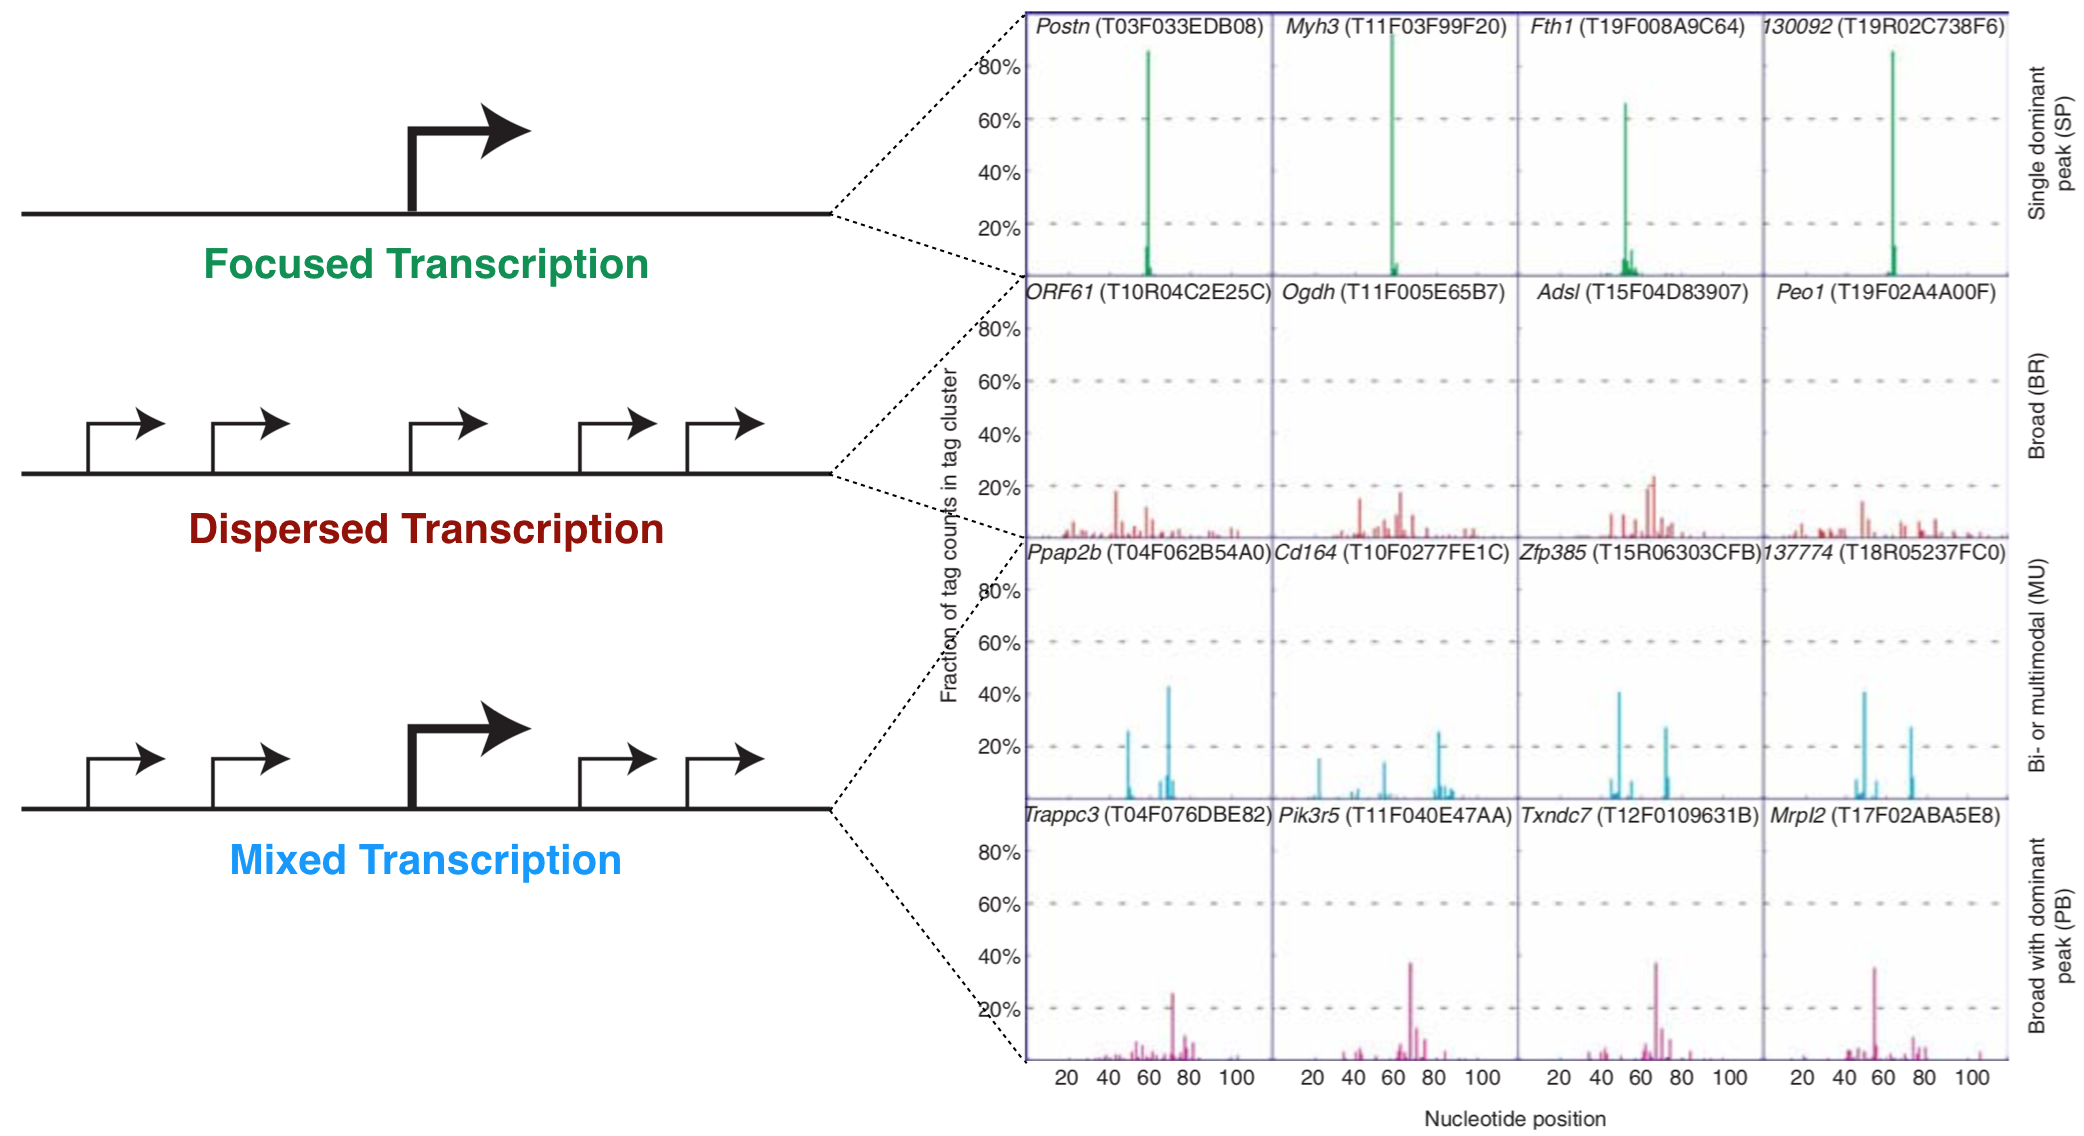
\includegraphics[width=1\linewidth]{static/images/TypesofPromoters}

}

\caption{The left schematic from Vo ngoc et al. 2017 illustrates the three main types of promoters that are found in animals: Focused, Dispersed and Mixed. The right image from Carninci et al. 2006 displays TSS seq data for a number of genes that illustrate each type of promoter.}\label{fig:promotertypes}
\end{figure}

Focused core promoters were the first described and are the best understood. In humans, they are about 80 nt in length and flank\footnote{extend both upstream and downstream of the TSS} the TSS, the so-called +1 position of transcription (Figure \ref{fig:80nt}). Each includes a set of short, DNA sequences called core promoter motifs\footnote{Sequence motifs are short, recurring patterns in DNA that are presumed to have a biological function. Often they indicate sequence-specific binding sites for proteins - D'haeseleer 2006}. These DNA motifs serve as binding sites for a subset of GTFs (namely TFIID and TFIIB). Once TFIID and TFIIB bind a focused core promoter, they recruit and stabilize other GTFs which together recruit and stabilize RNA polymerase II to the TSS. This large, multiprotien complex (called the preinitiation complex or PIC) initiates \textbf{basal levels of transcription}\footnote{formally defined as the level of transcription observed in an \emph{in vitro} transcription system where only DNA containing a core promoter, an RNA polymerase II and GTFs are added. In other words, the level of transcription that is detected in the absence of other proteins that enhance or repress transcription (so called transcription factors).}. In fact, GTFs are also called Basal Transcription Factors.

\begin{figure}

{\centering 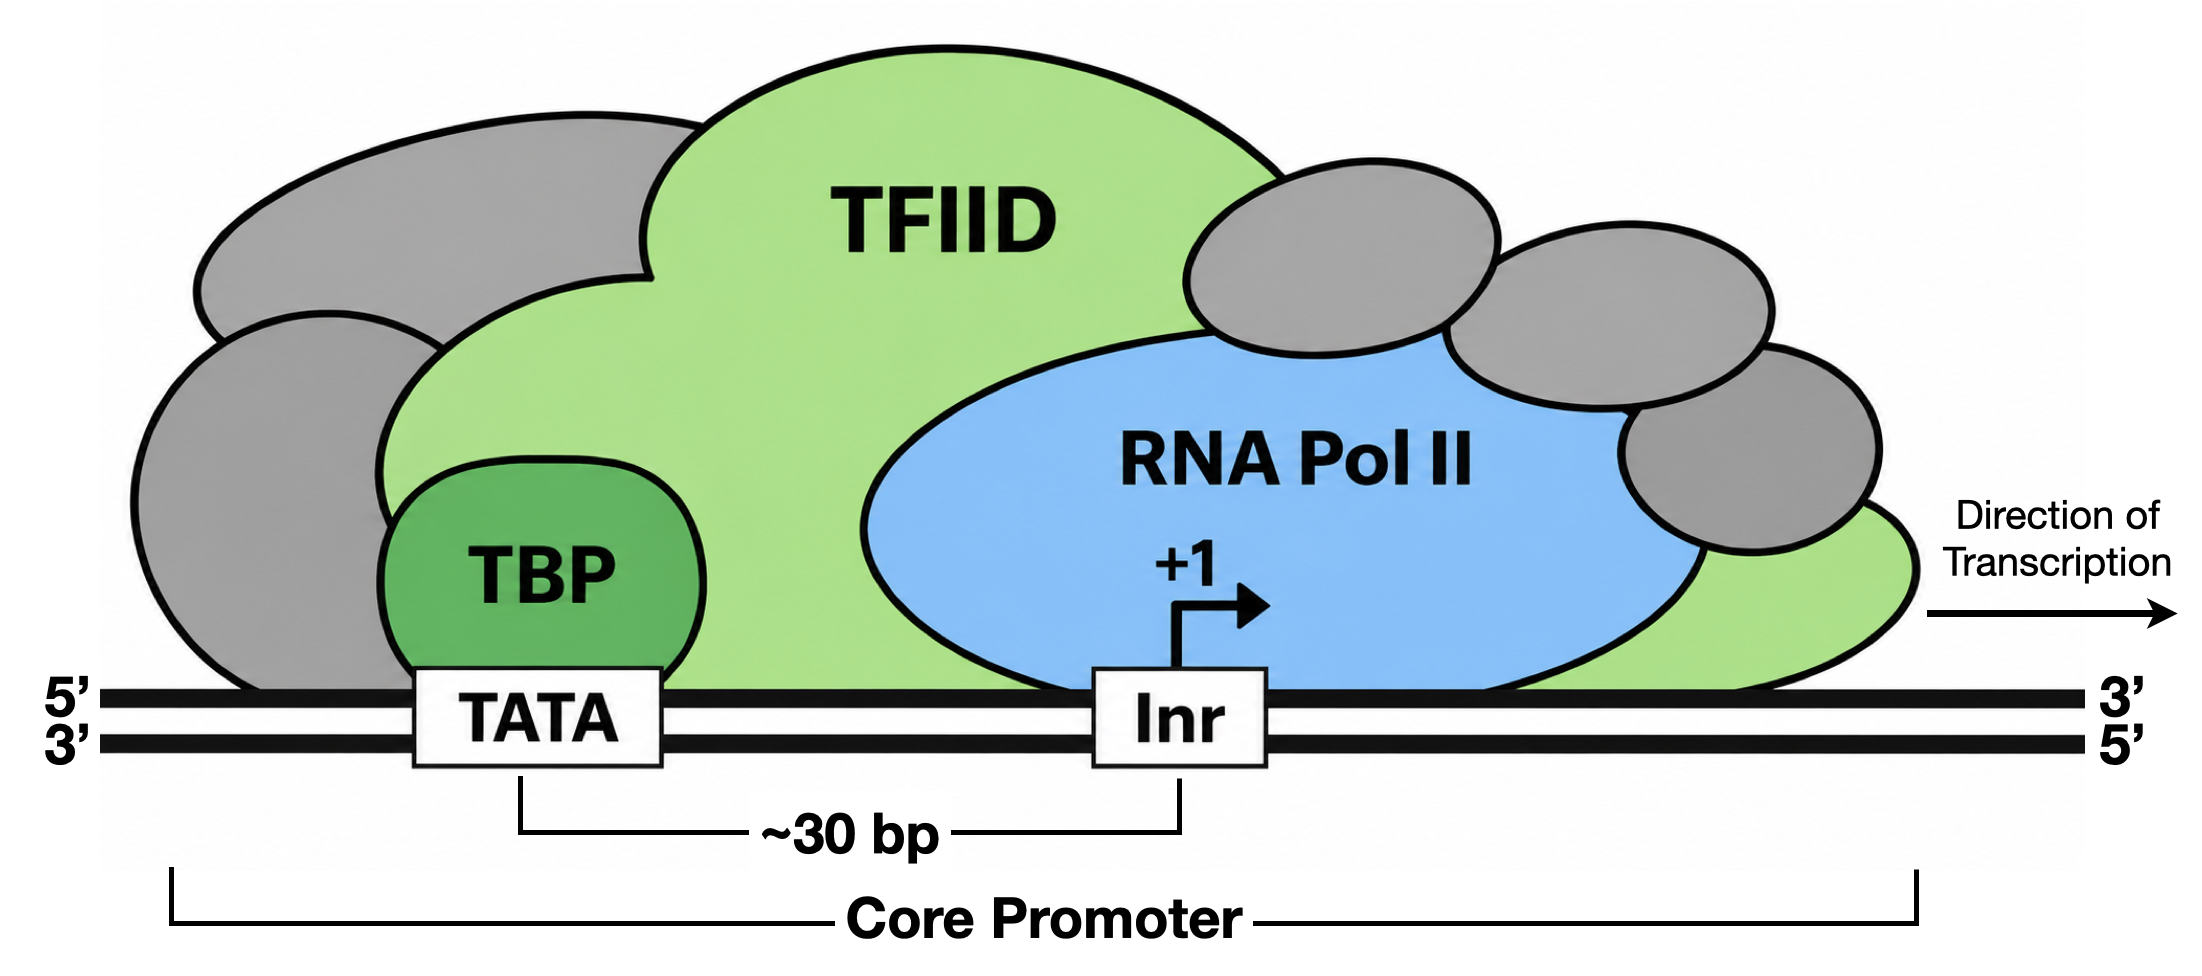
\includegraphics[width=0.75\linewidth]{static/images/FCorePromoter}

}

\caption{A schematic of a focused core promoter and the GTFs/RNA polymerase II that bind to it. The horizontal line is the genomic DNA. **TATA**, **Inr**, **MTE** and **DPE** are DNA sequence motifs positioned along the core promoter as shown. The **Inr** spans the TSS (+1) while the **TATA-box** is upstream and the **MTE** and **DPE** motifs are downstream.  Image from Danino et al. 2015.}\label{fig:80nt}
\end{figure}

The first core promoter motif identified was the \textbf{TATA-box}. The TATA-box recruits TFIID to the core promoter. Initially, the TATA-box was thought to be an essential motif that \emph{all} core promoters possess (Read any textbook). We now know they are only present in a minority of core promoters. For example, only 24\% of human genes have a TATA-box. The core promoter motif found \emph{most often} is the \textbf{Initiator} (Inr). This DNA motif spans the TSS and also recruits TFIID. That said, nearly half of human promoters lack both a TATA-box \emph{and} an Inr! The take home message? \textbf{\emph{There are no universal sequence motif required for transcription initiation in Eukaryotes.}} Not only that, but the sequence of each core promoter motif (i.e.~Inr) is somewhat variable. For example, the TATA-box in ACTA2 is \textbf{TATATAA} while the TATA-box in HERPUD1 is \textbf{TATAAAA} (two distinct human genes).

\hypertarget{what-is-a-consensus-sequence}{%
\section{What is a Consensus Sequence?}\label{what-is-a-consensus-sequence}}

By aligning a large number of well-characterized sequence motifs, one can search for sequence patterns and/or regions of sequence conservation\footnote{In evolutionary biology, conserved sequences are identical or similar sequences (DNA RNA or protein) across species (orthologous sequences) or within a genome (paralogous sequences). Conservation can indicate that a sequence has been maintained by natural selection. A highly conserved sequence suggests that it has remained relatively unchanged far back up the phylogenetic tree, and hence far back in geological time - paraphrased from the ``Conserved sequence'' article from Wikipedia}. Any region of conservation or pattern observed can then be written as a \textbf{consensus sequence}. A consensus sequence (also known as a \textbf{canonical sequence}) is defined as the ``the most frequent residues, either nucleotide or amino acid, that is found at each position in a multiple sequence alignment'' (Wikipedia). For a simple example, see Figure \ref{fig:consensusonly}. Notice that the multiple sequence alignment contains only G, A, T and C while the consensus sequence contains additional letters (Y, N and R). Y,N and R belong to an agreed upon list of \href{https://www.bioinformatics.org/sms/iupac.html}{\textbf{IUPAC nucleotide codes}} also known as IUPAC ambiguity codes. Here, Y = C or T, N = any nucleotide and R = G or A.

\begin{figure}

{\centering 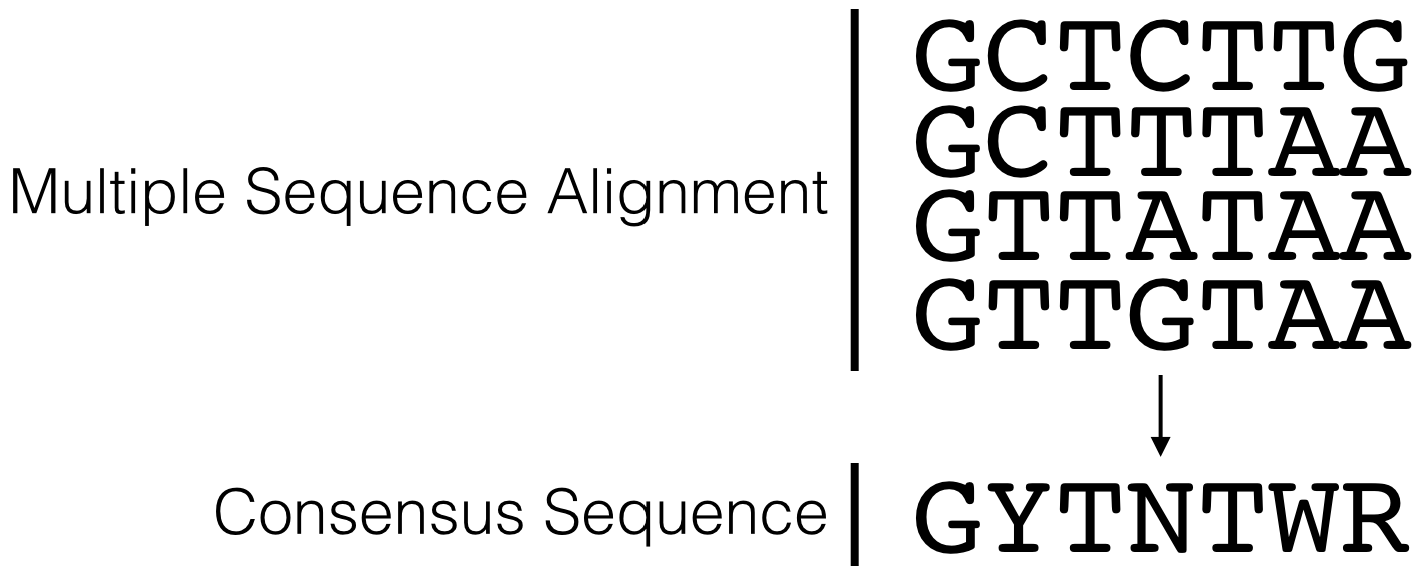
\includegraphics[width=0.5\linewidth]{static/images/MSA_Consensus}

}

\caption{This is a simple multiple sequence alignment (MSA) that includes only 4 sequences. The consensus sequence corresponding to this alignment is written directly below. It was created by examining the observed frequency of each nucleotide present in each column of sequence in the MSA.}\label{fig:consensusonly}
\end{figure}

Figure \ref{fig:CoreConsensus} lists the consensus sequences for each core promoter motif bound by TFIID in mammals. In this figure the \textbf{Inr} consensus sequence is listed as \textbf{BBCA(+1)BW} (where B = C, G or T; W= A or T and the A is at the +1 position of the TSS). That said, there have been so many exceptions to this consensus sequence that some argue it should be reduced to YR where Y = C or T and R is at the +1 position of the TSS (Haberle and Stark 2018)\footnote{The consensus sequence can vary depending on the size and quality of the sequence motif set used to create the multiple sequence alignment}!

\begin{figure}

{\centering 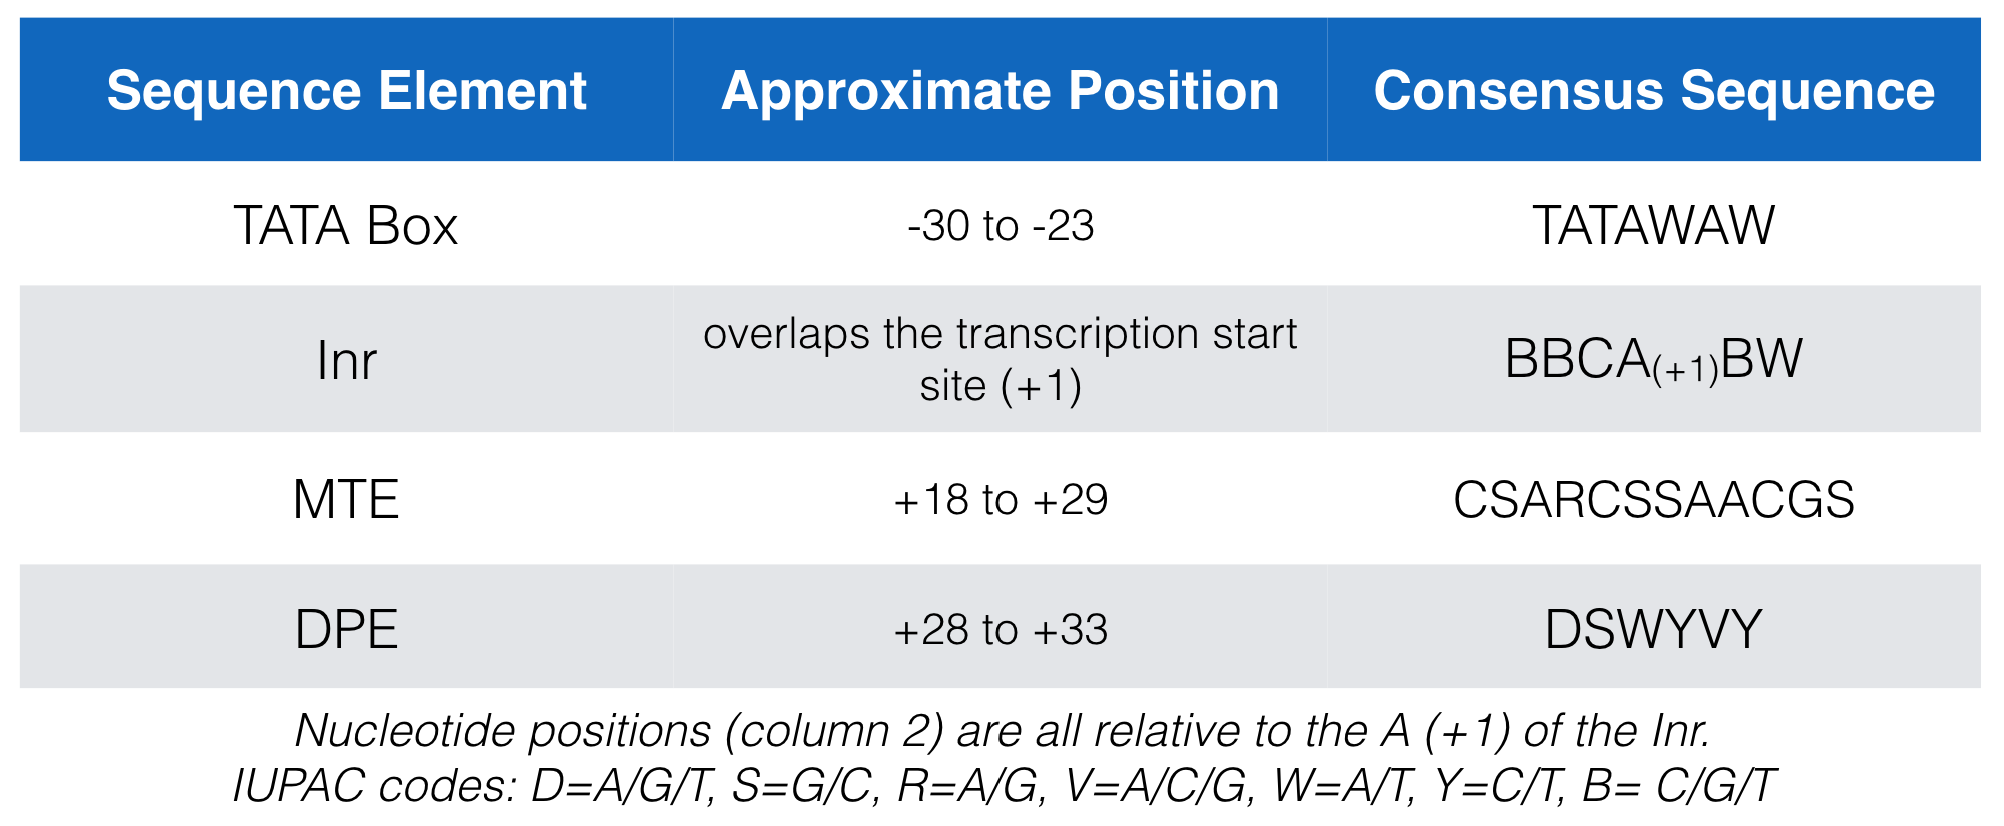
\includegraphics[width=0.75\linewidth]{static/images/CoreConsensusHuman}

}

\caption{A list of the consensus sequences for each core promoter motif bound by TFIID in mammals.}\label{fig:CoreConsensus}
\end{figure}

\hypertarget{searching-for-a-consensus-sequence}{%
\section{Searching for a consensus sequence}\label{searching-for-a-consensus-sequence}}

You can search for a consensus sequence containing IUPAC codes using an evidence track called, ``Short Match''. Before you open Short Match, open the saved \href{https://genome.ucsc.edu/s/megallegos/Biol\%20310\%3A\%20Module\%202\%20TSS\%2Dseq}{``TSS-Seq'' Session} then zoom in to view the sequence surrounding the TSS for BBS1. Now scroll down to find an evidence track entitled, \textbf{``Short Match''} (1) within the section entitled, \textbf{``Mapping and Sequencing''} (Figure \ref{fig:ShortMatch}). Change this evidence track from ``hide'' to ``pack'' and click ``refresh'' (2). A new evidence track will open (3). Click on the gray rectangle at left to open the track settings page for this track (4).

\begin{figure}

{\centering 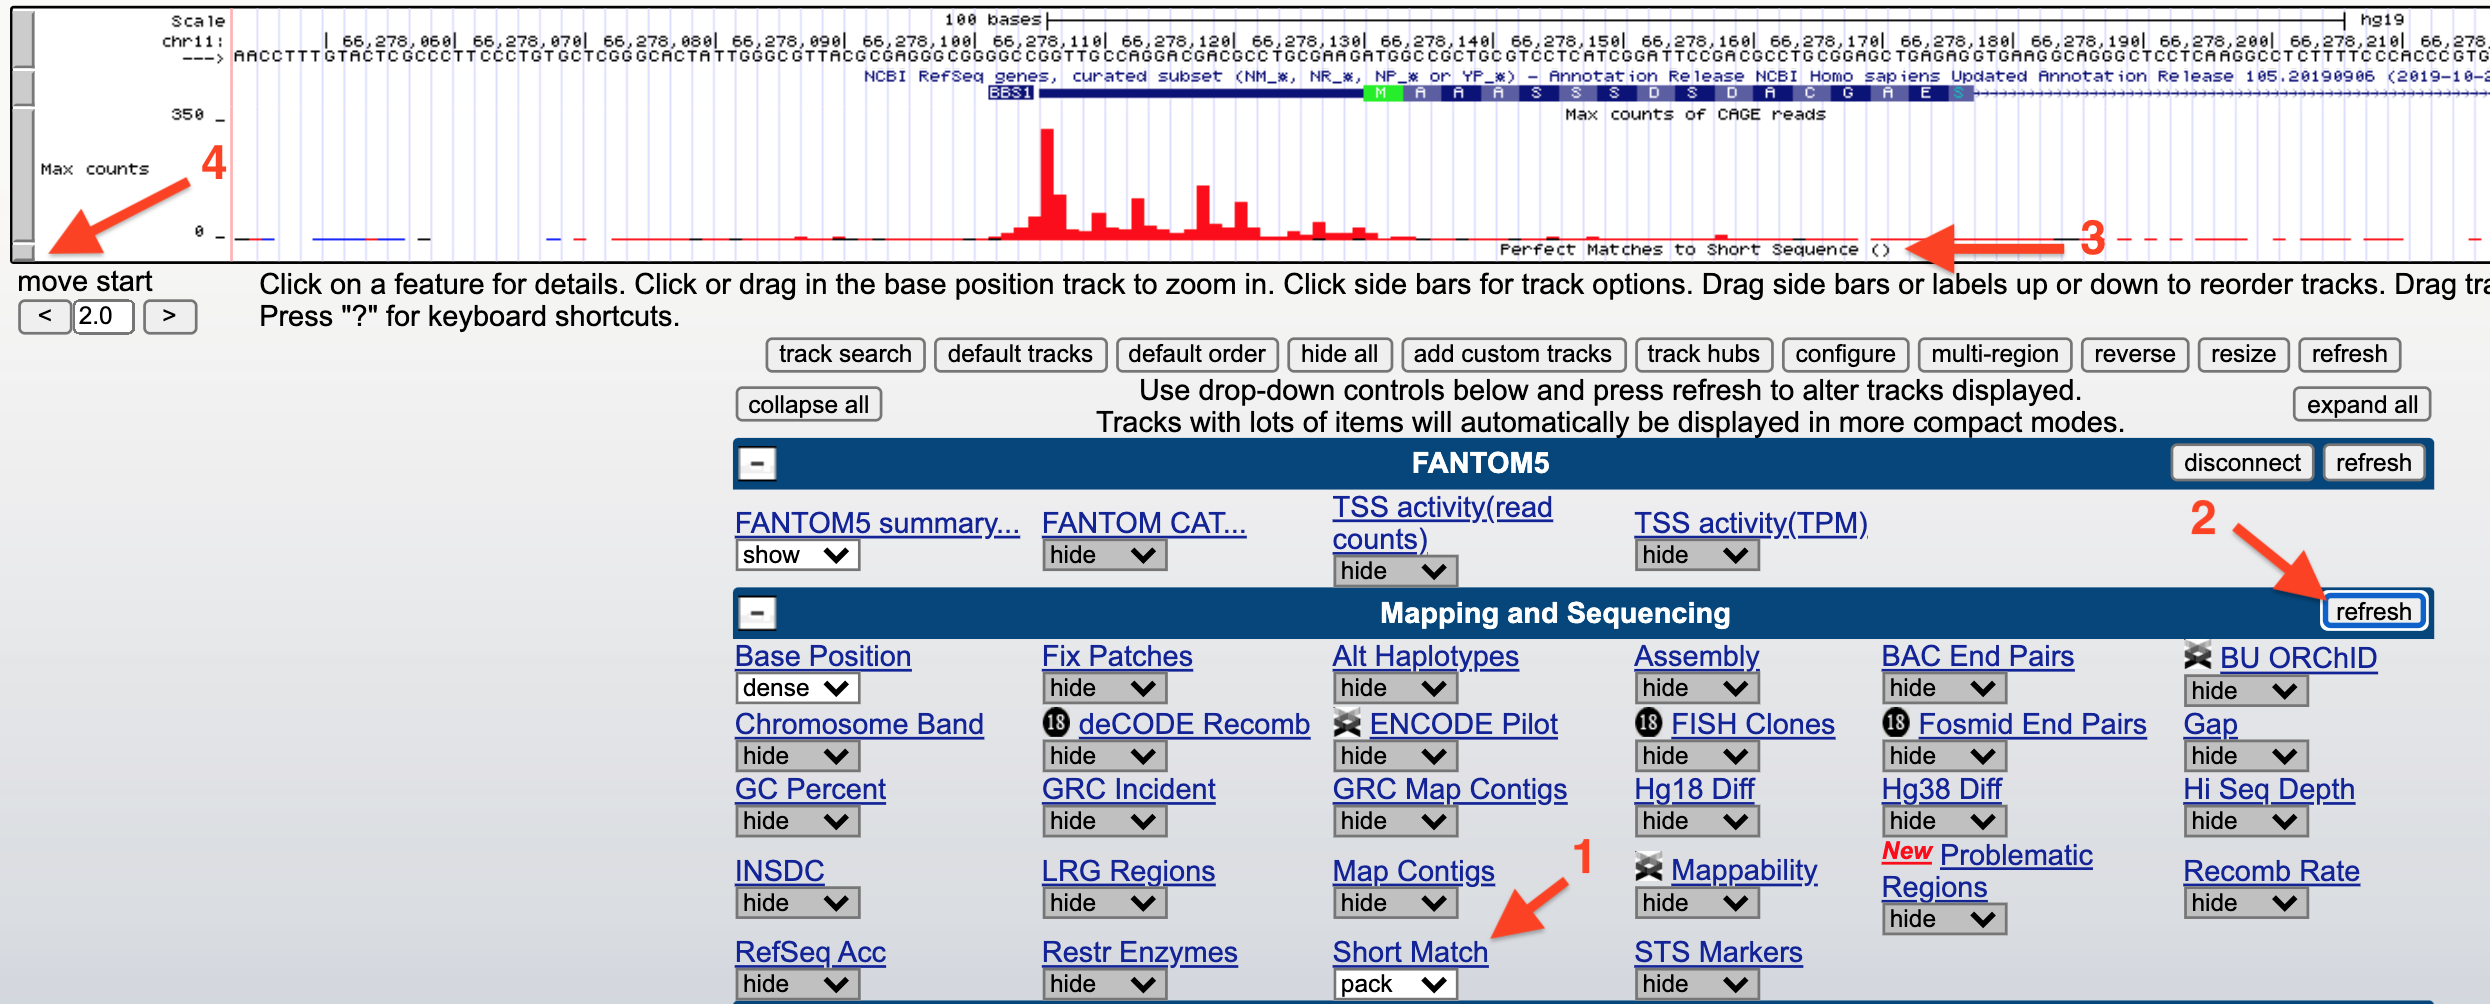
\includegraphics[width=1\linewidth]{static/images/ShortMatchSetup}

}

\caption{How to search for a consensus sequence: 1) change the **Short Match** evidence track from **hide** to **pack**. 2) Click **Refresh**. 3) A new evidence track will open. 4) Click on the gray rectangle to open the track settings page. Now see figure below.}\label{fig:ShortMatch}
\end{figure}

Finally, input any sequence (i.e.~ATG) into the search window (1) provided at the Track Settings page for Short Match (Figure \ref{fig:ShortMatchWindow}) then hit ``Submit'' (2).

\begin{figure}

{\centering 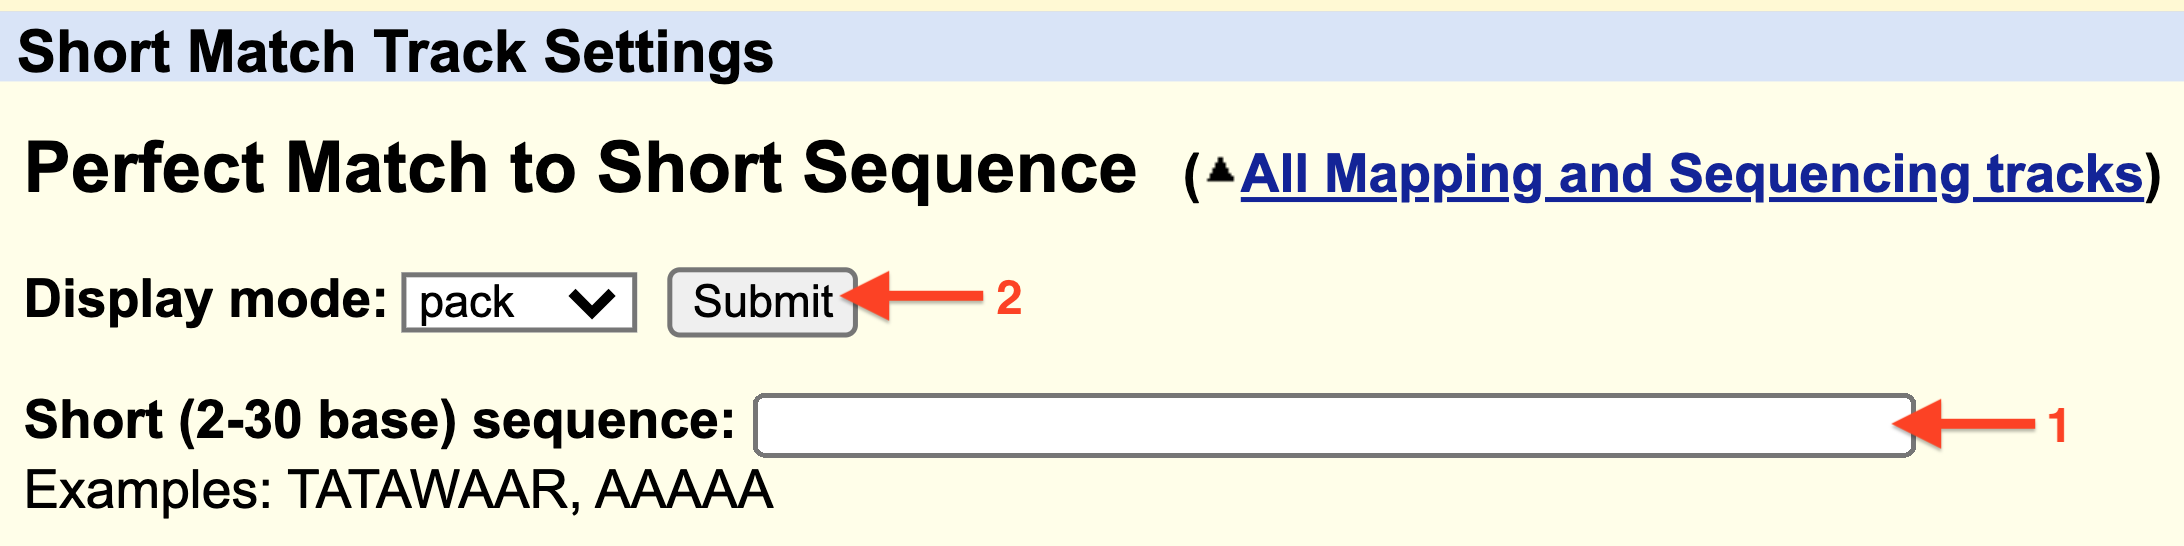
\includegraphics[width=0.6\linewidth]{static/images/EnterConsensus}

}

\caption{1) Enter a consensus sequence in the window provided. 2) Click Submit.}\label{fig:ShortMatchWindow}
\end{figure}

In Figure \ref{fig:InrEx}, I searched for the \textbf{Inr} consensus sequence, BBCA(+1)BW, in the genomic region surrounding the human gene (CCT2) TSS. Each match is displayed in the Short Match evidence track as a thick black line. The position (i.e.~69,979,214) and orientation (- or +) of each match is written on the left of each line. In this example, the putative\footnote{potential, possible, not experimentally proven without a doubt but some evidence in support of the possibility} Inr is the one highlighted with a red asterisk. What is my evidence? This is the only Inr consensus sequence that spans the predicted and experimentally-defined TSS at position 69,979,236. It is also found on the plus strand of the genomic DNA and CCT2 is a plus strand gene. Finally, the ``A'' of the consensus sequence is positioned at the predicted \emph{and} experimentally defined TSS (See red circle in Figure \ref{fig:InrEx}).

\begin{figure}

{\centering 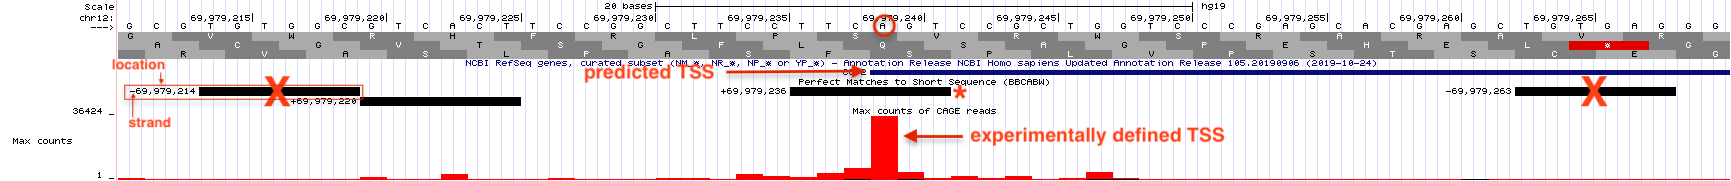
\includegraphics[width=1\linewidth]{static/images/Inr_Example}

}

\caption{Horizonatal black bars within the 'Short Match' evidence track describe the position of each consensus sequence (BBCA(+1)BW) found within this genomic region. Information about the precise nucleotide position and orientation is provided on the left (see boxed consensus on the left). The putative Inr for CCT2 is highlighted with a red asterix. This consensus sequence is found on the plus strand (same as CCT2) and is positioned directly below the experimentally defined TSS at 69,979,236 with the A at the putative +1 position.}\label{fig:InrEx}
\end{figure}

Now look what happens when I search for the degenerate \textbf{Inr} consensus sequence (YR). This is an extremely short consensus sequence and so many are expected to be present in any genomic region just by chance. That said, ALL the motifs found by Short Match are labeled as + strand!!! You should know intuitively this is impossible. There MUST be YR sequences on the bottom strand, too. In fact, Y (C/T) is complementary to R (G/A). Thus, where a YR sequence is found on the plus strand a YR sequence will \emph{always} be found on the bottom strand. You can see this for yourself in Figure \ref{fig:YR}. Remember to read the bottom strand from right to left (5' to 3'). For example, a CA dinucleotide in the top strand is a YR consensus sequence but so is its complementary sequence in the bottom strand: TG.

\begin{figure}

{\centering 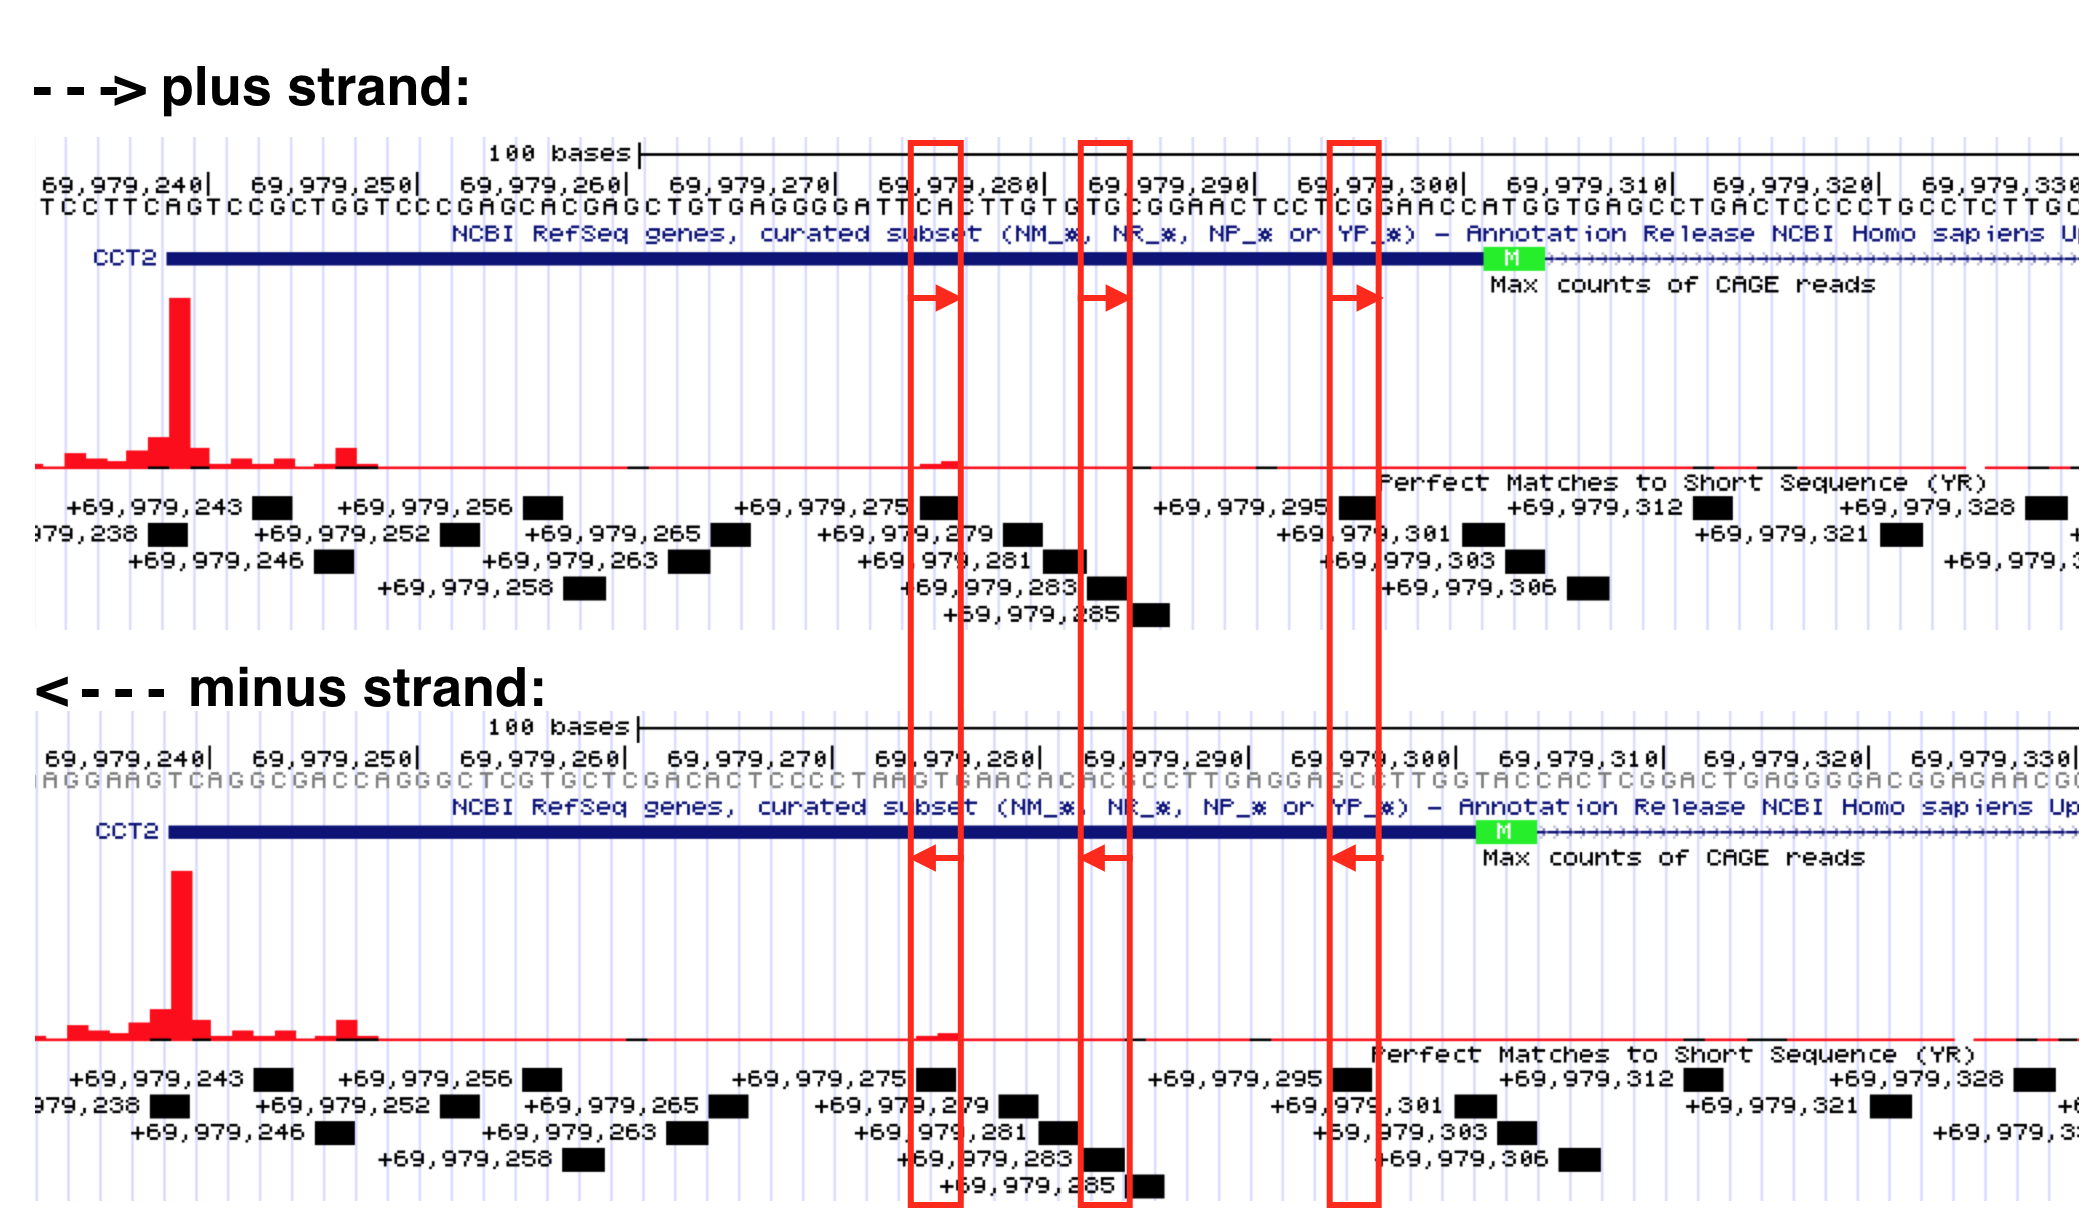
\includegraphics[width=1\linewidth]{static/images/YRcomp}

}

\caption{Select YR consensus sequences identified by the Short Match evidence track are boxed in red. Recall, Y = C or T while R=G or A. If you read the top strand sequence (from left to right) you can confirm that each is a YR consensus sequence. If you read the sequence (from right to left) for the exact same position in the minus strand, you will see it is also a YR sequence. Why do they label all YR Short Matches as plus strand? Convenience? I don't know.}\label{fig:YR}
\end{figure}

\hypertarget{test-your-understanding-15}{%
\subsection{\texorpdfstring{\href{https://docs.google.com/forms/d/e/1FAIpQLSc4NEqD8He-jer_Qa2zWL5ruhK_J8FJxp5MJ8DOL14UpEimDA/viewform?usp=sf_link}{Test your understanding}}{Test your understanding}}\label{test-your-understanding-15}}

\begin{itemize}
\tightlist
\item
  \emph{Use \href{https://www.bioinformatics.org/sms/iupac.html}{IUPAC nucleotide codes} to rewrite the following consensus sequence: T/A, G/A/C, A, G/A, C/T, T, G/A/T/C, T (where ``/'' = ``or'').}
\end{itemize}

\textbf{For the following questions start with the \href{https://genome.ucsc.edu/s/megallegos/Biol\%20310\%3A\%20Module\%202\%20TSS\%2Dseq}{``TSS-Seq''} session link, zoom into the region containing the BBS1 TSS then change the Short Match evidence track from ``hide'' to ``pack''. Remember the core promoter is defined as the region that includes the TSS plus 40 nt upstream and downstream (80 nt in total).}

\begin{itemize}
\tightlist
\item
  \emph{Use the ShortMatch evidence track to search for a canonical TATA-box consensus sequence (TATAWAW) within the BBS1 core promoter region. If one or more are found,}
  -- \emph{Are any on the plus strand as expected?}
  -- \emph{Are any of the plus strand motifs positioned approximately 30 nt upstream of the predicted TSS as expected?}
\item
  \emph{Use the Short Match evidence track to search for a canonical Inr consensus sequence (BBCABW) within the BBS1 core promoter region. If one or more are found,}
  -- \emph{Are any on the plus strand as expected?}
  -- \emph{Do any of the plus strand motifs span the TSS as expected?}
\item
  \emph{If a BBCABW consensus sequence is NOT found spanning the the TSS of BBS1, is there a degenerate Inr consensus sequence (YR) spanning the TSS as expected?}
\item
  \emph{Use the Short Match evidence track to search for a canonical MTE consensus sequence (CSARCSSAACGS) within the BBS1 core promoter region. If one or more are found,}
  -- \emph{Are any on the plus strand as expected?}
  -- \emph{Are any of the plus strand motifs positioned downstream of the TSS as expected?}
\item
  \emph{Use the Short Match evidence track to search for a canonical DPE consensus sequence (DSWYVY) within the BBS1 core promoter region. If one or more are found,}
  -- \emph{Are any on the plus strand as expected?}
  -- \emph{Are any of the plus strand motifs positioned downstream of the TSS as expected?}
\end{itemize}

\hypertarget{test-your-understanding-16}{%
\subsection{\texorpdfstring{\href{https://docs.google.com/forms/d/e/1FAIpQLSfMGNjfgSnl-GVNBXiKnLIA0yDvAZKE9kAO11CqdXAPRDa3Gw/viewform?usp=sf_link}{Test your understanding}}{Test your understanding}}\label{test-your-understanding-16}}

\textbf{For the following questions start with the \href{https://genome.ucsc.edu/s/megallegos/Biol\%20310\%3A\%20Module\%202\%20TSS\%2Dseq}{``TSS-Seq''} session link, zoom into the region containing the MYH3 TSS then change the Short Match evidence track from ``hide'' to ``pack''. Remember the core promoter is defined as the region that includes the TSS plus 40 nt upstream and downstream (80 nt in total). Also, MYH3 is a minus strand gene.}

\begin{itemize}
\tightlist
\item
  \emph{Use the ShortMatch evidence track to search for a canonical TATA-box consensus sequence (TATAWAW) within the MYH3 core promoter region. If one or more are found,}
  -- \emph{Are any on the minus strand as expected?}
  -- \emph{Are any of the minus strand motifs positioned approximately 30 nt upstream of the predicted TSS as expected?}
\item
  \emph{Use the Short Match evidence track to search for a canonical Inr consensus sequence (BBCABW) within the MYH3 core promoter region. If one or more are found,}
  -- \emph{Are any on the minus strand as expected?}
  -- \emph{Do any of the minus strand motifs span the TSS as expected?}
\item
  \emph{If a BBCABW consensus sequence is NOT found spanning the the TSS of MYH3, is there a degenerate Inr consensus sequence (YR) spanning the TSS as expected?}
\item
  \emph{Use the Short Match evidence track to search for a canonical MTE consensus sequence (CSARCSSAACGS) within the MYH3 core promoter region. If one or more are found,}
  -- \emph{Are any on the minus strand as expected?}
  -- \emph{Are any of the minus strand motifs positioned downstream of the TSS as expected?}
\item
  \emph{Use the Short Match evidence track to search for a canonical DPE consensus sequence (DSWYVY) within the MYH3 core promoter region. If one or more are found,}
  -- \emph{Are any on the minus strand as expected?}
  -- \emph{Are any of the minus strand motifs positioned downstream of the TSS as expected?}
\end{itemize}

\hypertarget{sequence-logos}{%
\section{Sequence Logos}\label{sequence-logos}}

Sequence conservation, trends and patterns revealed by a multiple sequence alignment (MSA) can also be visualized with a ``sequence logo'' where the predominant residue is drawn as the tallest and placed at the top among all the residues found at a given position in an alignment. For example, let's say at position 3 of an MSA there is a T in every single sequence (For a simple example see Figure \ref{fig:MSAdisplays}). In a sequence logo, this would be displayed as a T of maximum height (illustrating that the T in that position is invariant and important). Now let's say position 6 has an A in 75\% of the sequences and a T in the remaining 25\%. At this position of a sequence logo you would see an A on top of the T, the A would be proportionally larger than the T but the overall height of the two letters combined would be shorter than the T in position 3. And in the extreme case where G, A, T or C are found in equal proportion that position in the sequence logo would be left blank (see position 4 in Figure \ref{fig:MSAdisplays})! This indicates that that position of the alignment is utterly uninformative. In a traditional consensus sequence using IUPAC codes, this would be written as ``N'' for any nucleotide. One can also draw a sequence logo using \emph{frequency} for the Y-axis. This type of sequence logo is more intuitive but many think it is less able to emphasize important sequence trends. What do you think?

\begin{figure}

{\centering 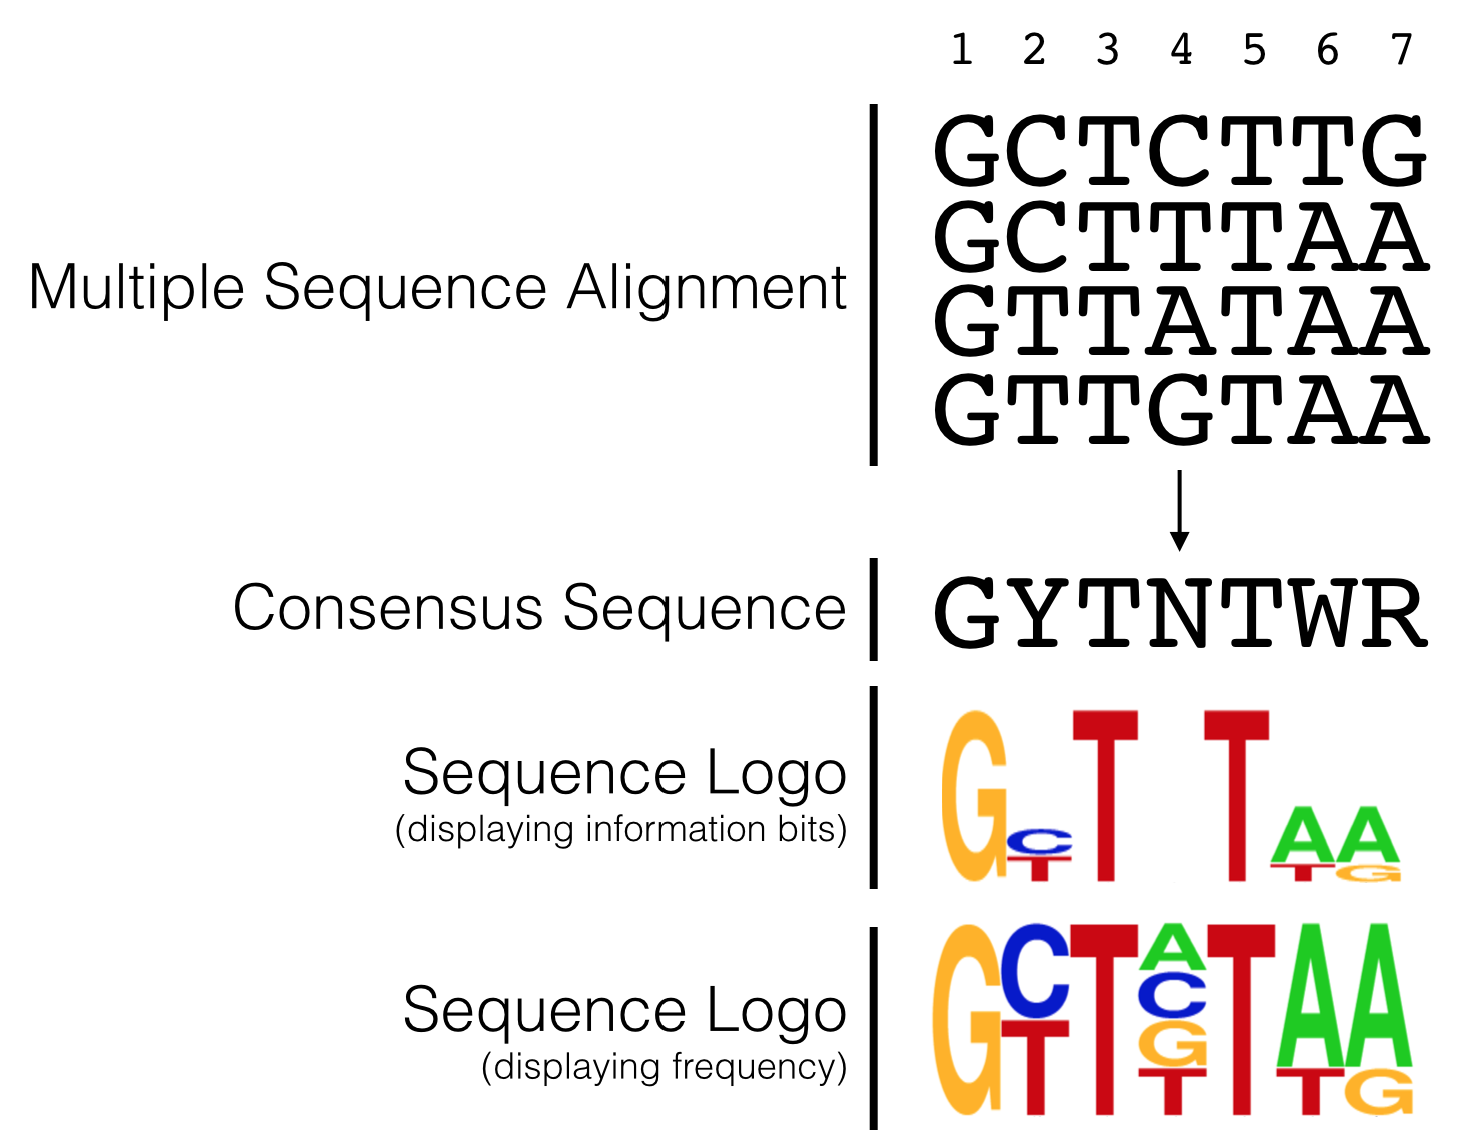
\includegraphics[width=0.5\linewidth]{static/images/MSA_Con_SeqLogo}

}

\caption{The hypothetical multiple sequence alignment is redrawn as a consensus sequence including IUPAC codes, or as a sequence logo with either information bits or frequency as the Y axis.}\label{fig:MSAdisplays}
\end{figure}

In 2006, Carninci et al.~performed an unbiased, systematic analysis of \emph{all} core promoter sequences identified by TSS-seq data obtained from RNA extracted multiple human tissue types. In their analysis confirmed the diversity of promoter types classifying them into four discrete categories (Figure \ref{fig:promotertypes}) including the two extremes: Single Predominant Peak (SP) and Broad Peak (BR). They aligned core promoter sequences by category, placing the +1 position of the TSS in a single column then adding the surrounding sequences to create a large multiple sequence alignment. They then created a sequence logo for each multiple sequence alignment (MSA). Two are displayed in Figure \ref{fig:SequenceLogo}. As you can see, the SP promoters are more likely to contain a TATA-box-like sequence about 30 nt upstream of the so-called Inr and there is a strong bias for a purine (G or A) at the +1 position of the TSS. Broad Peak (BR) promoters were found to be similar to SP promoters only in that they have a a strong bias for a purine at the +1 position of the TSS but they clearly lack a TATA-box and are enriched overall with Gs and Cs. Take home message: \textbf{There are no universal promoter motifs. There may be sequence trends but there is a tremendous amount of sequence diversity at the core promoter.} Clearly it would be very difficult to identify genes based solely on the presence of conserved core promoter sequence motifs.

What I have not discussed in this chapter is how a cell ``knows'' when and which tissue a gene should be transcribed. That requires far more than the core promoter sequence and can sometimes involves DNA sequence on other chromosomes! This is a topic for another course.

\begin{figure}

{\centering 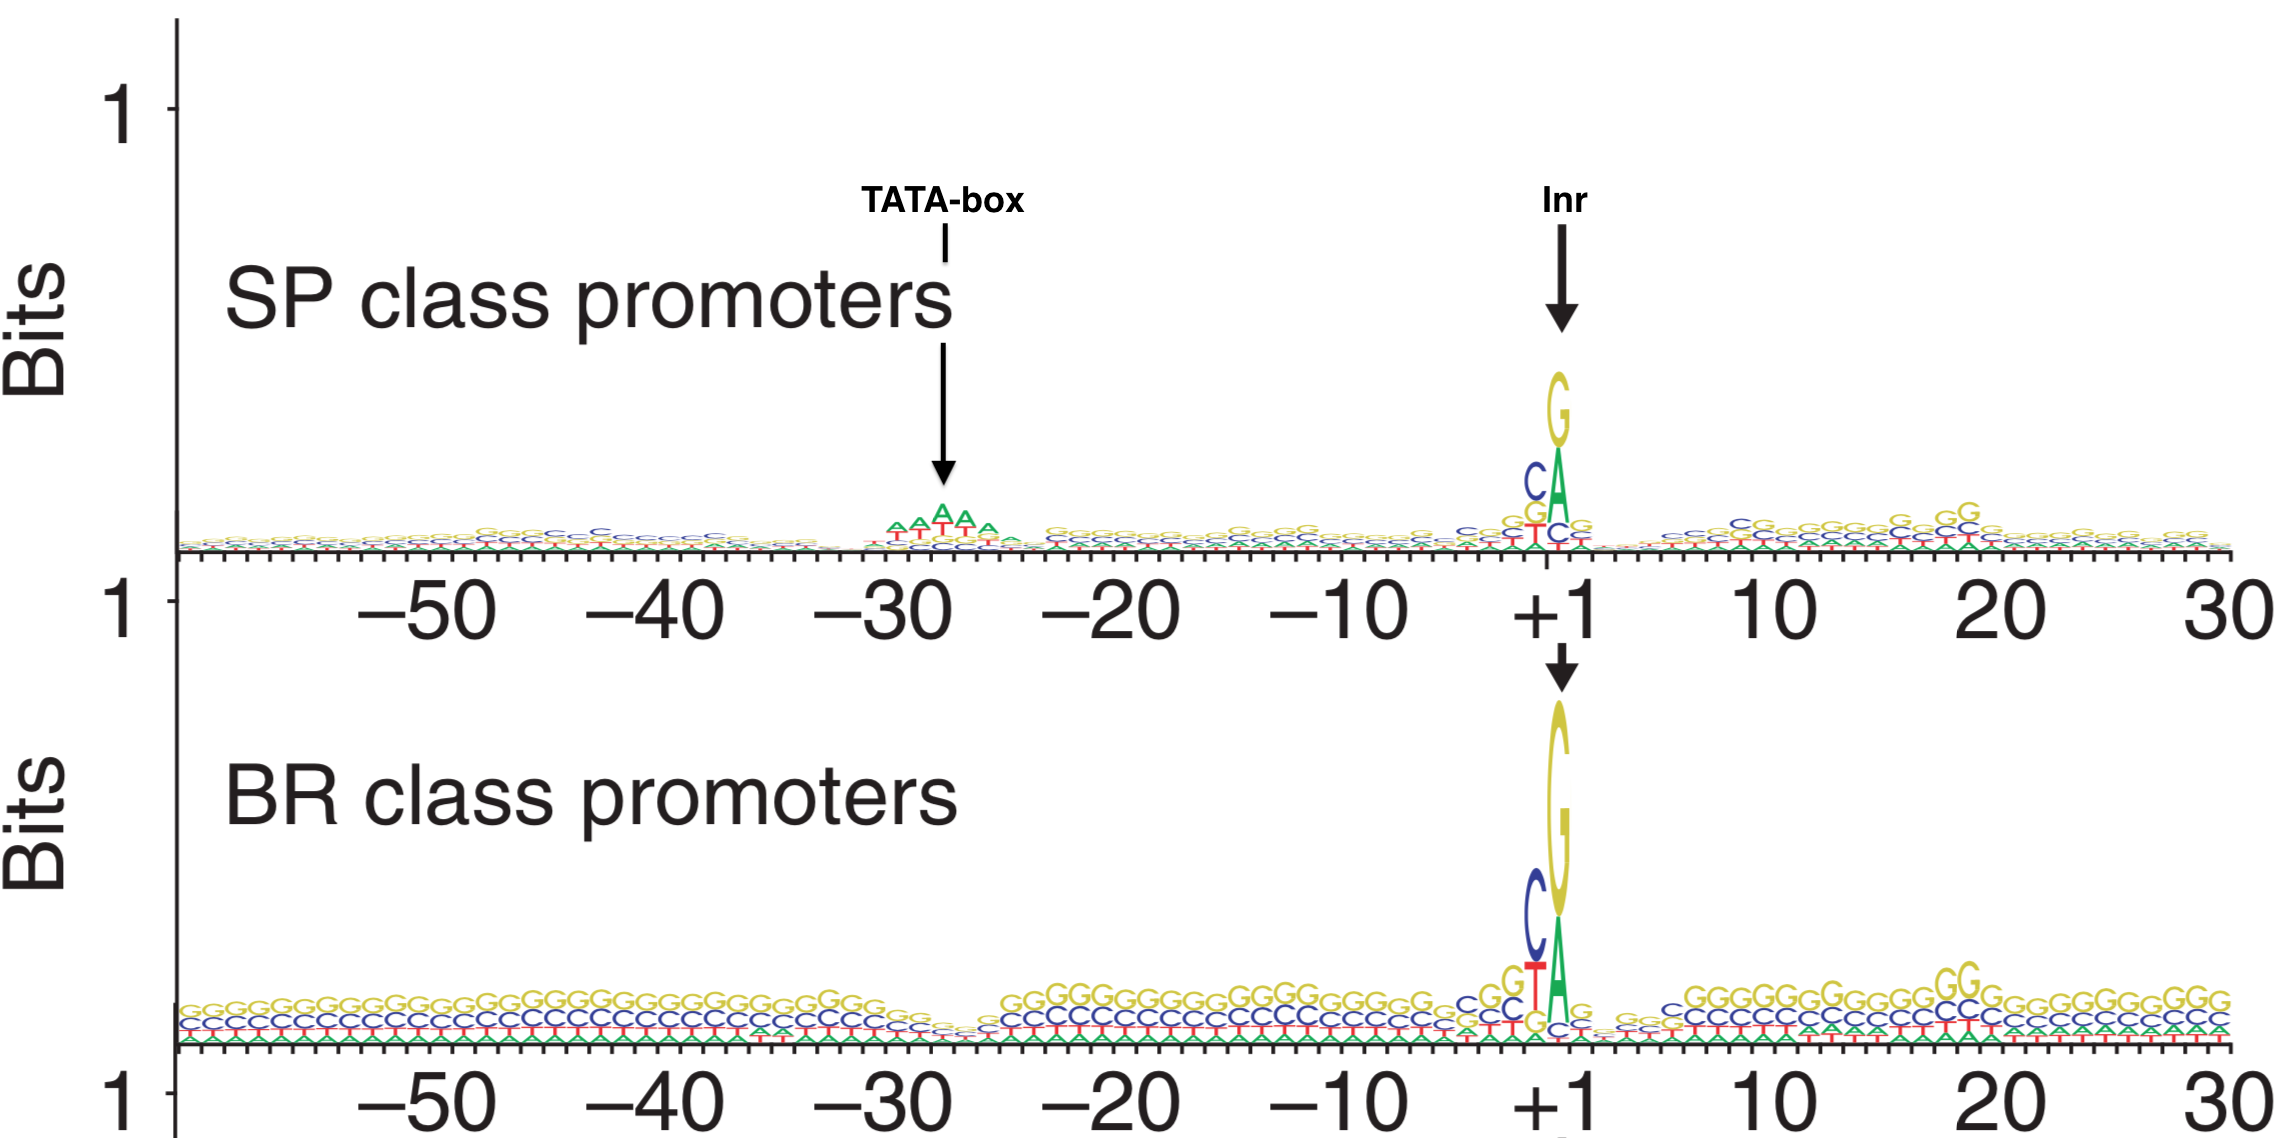
\includegraphics[width=1\linewidth]{static/images/SequenceLogo_SP_BR}

}

\caption{Sequence Logos for Single Predominent Peak (SP) and Broad Peak (BR) promoter types. The position of the TATA-box and Inr are highlighted in the SP class of promoters. The +1 represents the TSS.}\label{fig:SequenceLogo}
\end{figure}

\hypertarget{test-your-understanding-17}{%
\subsection{\texorpdfstring{\href{https://docs.google.com/forms/d/e/1FAIpQLScT6tA9iWRqeRGbT3ELUc-RedNhDYg2LuCceRZeTSsNX0A6_g/viewform?usp=sf_link}{Test Your Understanding}}{Test Your Understanding}}\label{test-your-understanding-17}}

\textbf{Below is a sequence logo drawn from a multiple sequence alignment (MSA) involving a subset of well-characterized metazoan TATA-boxes\footnote{metazoan means animal} (Haberle and Stark, 2018).}

\begin{center}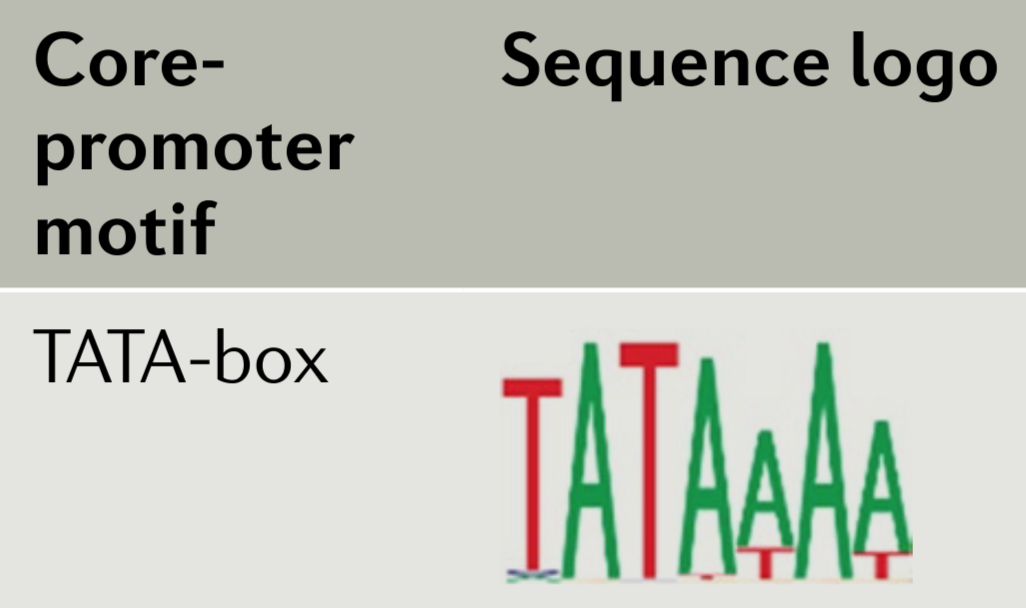
\includegraphics[width=0.3\linewidth]{static/images/SeqLogoTATA} \end{center}

\begin{itemize}
\tightlist
\item
  \emph{In this manual, I write the consensus sequence for the TATA-box as TATAWAW. It has also been written as TATAWAAR with an A in the 7th position (Kadonaga 2012). Based on the sequence logo above, which consensus sequence is a better match (ignore the ``R'' in TATAWAAR when you answer this question as the sequence logo above is only 7 nt long)}
\item
  \emph{In both consensus sequences (TATAWAW and TATAWAAR), an A is placed in the fourth position. Given the sequence logo above what other letter is sometimes present in that position?}
\item
  \emph{In the fifth position of both consensus sequences is a W. This implies that a T or A are possible at this position. Given the sequence logo how frequently is the T vs the A observed?}
\end{itemize}

© 2019, Maria Gallegos. All rights reserved.

\hypertarget{rna-motifs-for-rna-processing-and-translation}{%
\chapter{\texorpdfstring{\emph{RNA motifs for RNA processing and translation}}{RNA motifs for RNA processing and translation}}\label{rna-motifs-for-rna-processing-and-translation}}

An RNA transcript cannot be \textbf{translated} as is. It must first be modified to produce a mature messenger RNA (mRNA). This modification process is called \textbf{pre-mRNA processing} and includes:

\begin{enumerate}
\def\labelenumi{\arabic{enumi}.}
\tightlist
\item
  The addition of a 5' methyl guanosine cap (\textbf{5' cap}).
\item
  The removal of introns (\textbf{splicing}).
\item
  \textbf{RNA cleavage} (to terminate transcription) and
\item
  The addition of a \textbf{poly(A) tail}.
\end{enumerate}

In fact, pol II transcription and RNA processing are closely coordinated with mRNA transport out of the nucleus. This ensures that only fully processed mRNAs make it to the cytoplasm for translation. In this chapter, we will learn about RNA sequence motifs that are required for pre-mRNA processing (in the nucleus) \emph{and} translation (in the cytoplasm). Again we will focus on BBS1 as our model gene to answer the question: Does BBS1 have all the sequence elements required for these processes. Let's see. To follow along with the text and to answer ``Test Your Understanding'' questions, start with the \href{https://genome.ucsc.edu/s/megallegos/Biol\%20310\%20Module\%201}{``Gene structure''} session.

\hypertarget{the-addition-of-a-5-guanosine-cap}{%
\section{The Addition of a 5' guanosine cap}\label{the-addition-of-a-5-guanosine-cap}}

The first step in pre-mRNA processing involves the addition of a 5' cap structure. A modified guanosine ribonucleotide is covalently attached to the first \emph{templated} ribonucleotide of all pre-mRNA transcripts once the 5' end of the nascent\footnote{new, just coming into existence} RNA chain dissociates from the genomic DNA (Figure \ref{fig:5cap}). There are no specific sequences required for this event to occur. As a result, all mature mRNAs begin with a ribonucleotide G. Now let's review the mRNA sequence of a random human gene: SPTBN2 (\href{https://www.ncbi.nlm.nih.gov/nuccore/NM_006946.4?report=fasta}{NM\_006946.4}). Notice that the mRNA sequence (displayed in FASTA format) begins with an A! Wait! Didn't I just say that all mRNAs are capped with a modified guanosine ribonucleotide? While this is true, sequence databases start mRNA sequence with the first \emph{templated} ribonucleotide instead. They assume you know a ``G'' is added to the 5' end of the emerging RNA during transcription.

\begin{figure}

{\centering 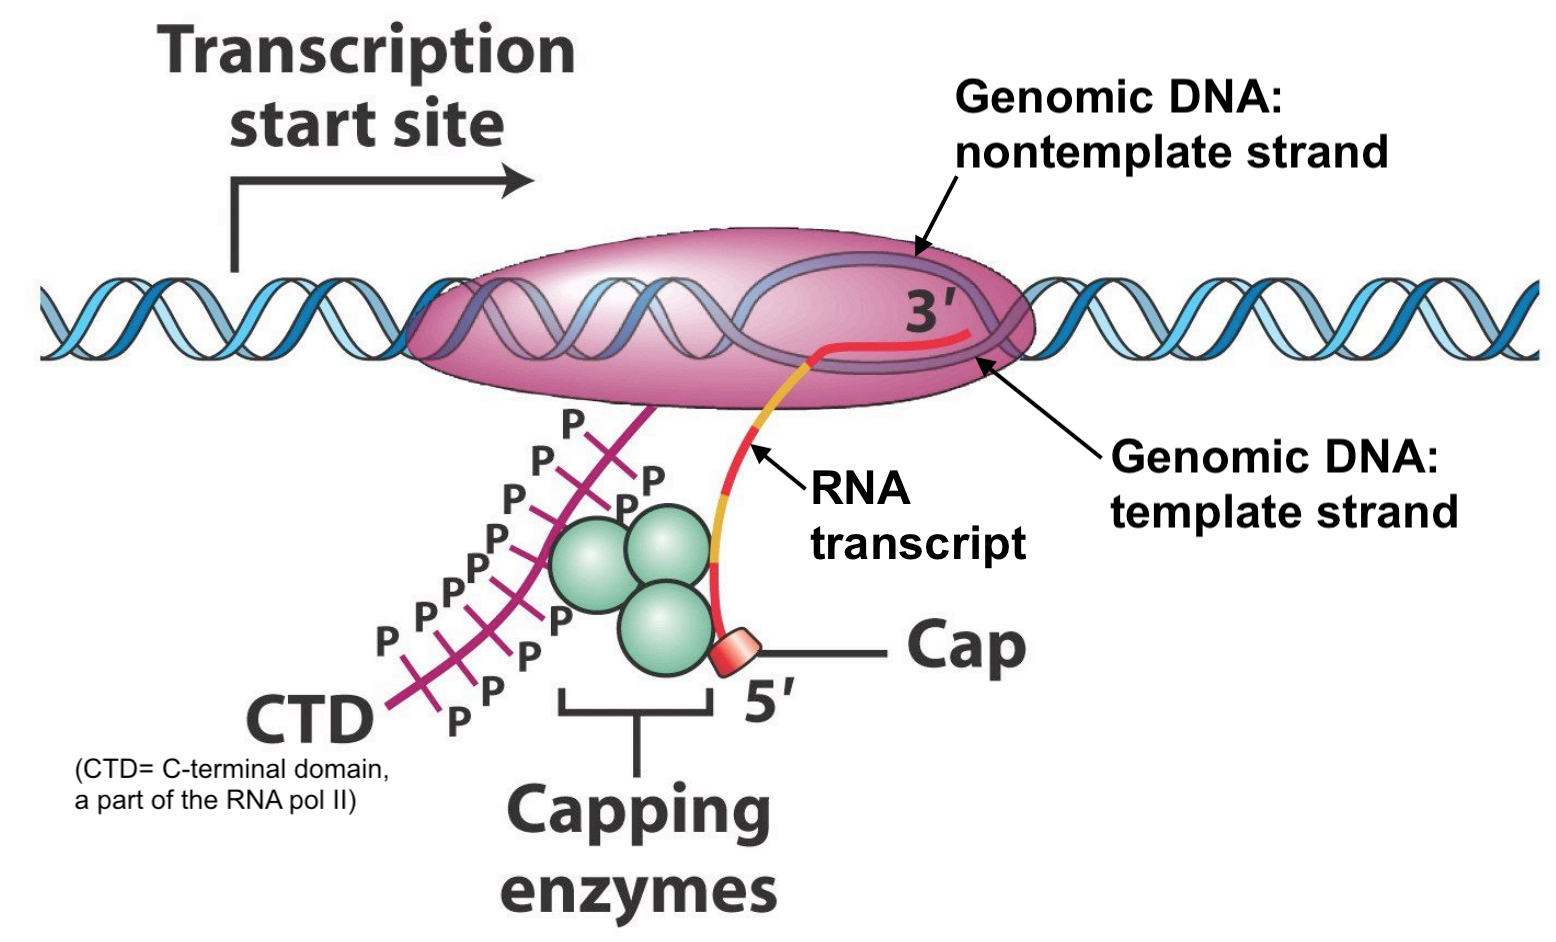
\includegraphics[width=0.5\linewidth]{static/images/capping}

}

\caption{Original image from Peter J. Russell, iGenetics: Copyright © Pearson Education, Inc., publishing as Benjamin Cummings. Additional annotation added here for clarity.}\label{fig:5cap}
\end{figure}

\hypertarget{splicing}{%
\section{Splicing}\label{splicing}}

The second step in pre-mRNA processing is the removal or splicing out of introns and the merging or joining of adjacent exons. Introns are spliced out by the splicing machinery also known as the \textbf{spliceosome}, a large complex of proteins and RNAs. To initiate splicing, the spliceosome must recognize and bind to the 5' and 3' ends of each intron in the RNA transcript\footnote{also known as splice site junctions}. Then the spliceosome pulls the two adjacent exons together to facilitate the excision of the intron and fusion of the two exons (Figure \ref{fig:splicingmachinery}).

\begin{figure}

{\centering \includegraphics[width=0.5\linewidth]{static/images/splicing}

}

\caption{From Schneider et al. 2010. The spliceosome includes the U1, U2, U4, U5 and U6 small nuclear ribonucleoproteins (snRNPs). SR proteins (in red) and splicing enhancer sequences within the exon are also utilized for accurate splicing. THis is particularly important with long introns.}\label{fig:splicingmachinery}
\end{figure}

To see if specific RNA motifs are required for splicing, scientists aligned the 5' and 3' ends of thousands of introns one on top of the other creating a multiple sequence alignment to allow patterns of sequence conservation to emerge. The result of one such analysis is displayed below as a sequence logo (Figure \ref{fig:intronsequencelogo}). This particular sequence logo was created by aligning the 5' and 3' ends of \emph{all} human introns below a certain size. Do you see which nucleotides are invariant? This sequence logo clearly illustrates that splicing DOES require specific sequences for the spliceosome to recognize the 5' and 3' ends of the intron.

\begin{figure}

{\centering 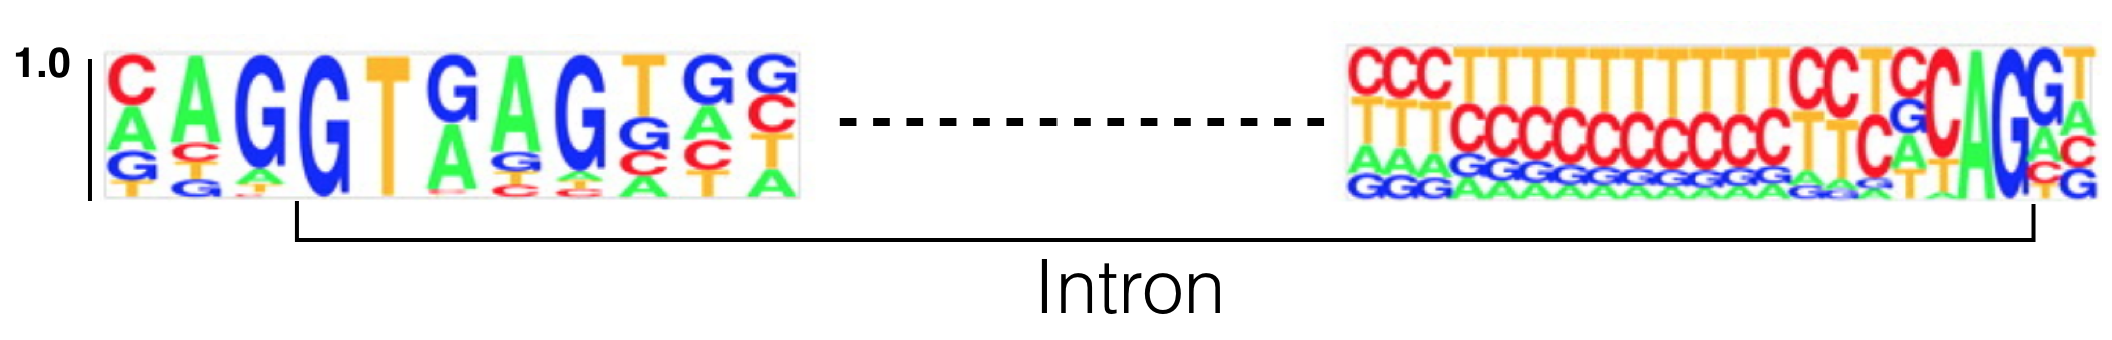
\includegraphics[width=1\linewidth]{static/images/intronlogo}

}

\caption{This sequence logo was created by aligning 5' and 3' splice site junctions of *all* human introns below a certain size. The Y axis represents frequency. The intron is bracketed as shown. Modified from Lim and Burge 2001.}\label{fig:intronsequencelogo}
\end{figure}

\hypertarget{test-your-understanding-18}{%
\subsection{\texorpdfstring{\href{https://docs.google.com/forms/d/e/1FAIpQLSdLNDxLkxtahAy52dMlJSxcah4fFO6CYDbCJRAqizq7ux14IQ/viewform?usp=sf_link}{Test Your Understanding}}{Test Your Understanding}}\label{test-your-understanding-18}}

\textbf{Use the sequence logo in Figure \ref{fig:intronsequencelogo} to answer the following questions (Note: The Y axis represents frequency):}

\begin{itemize}
\tightlist
\item
  \emph{Based on what you know so far about how sequence is typically displayed, where is the 5' splice site? On the left or right side of the figure?}
\item
  \emph{This sequence logo demonstrates that there are two nucleotides that are found at the 5' end of nearly 100\% of all introns. This is called the 5' splice site (5' SS or 5' donor site). Based on this sequence logo, what is the sequence of the 5' splice site?}
\item
  \emph{This sequence logo demonstrates that there are two nucleotides that are found at the 3' end of nearly 100\% of all introns. This is called the 3' splice site (3' SS or 3' acceptor site). Based on this sequence logo, what is the sequence of the 3' splice site?}
\item
  \emph{Based on this sequence logo, what is the probability of observing a G immediately 5' (upstream) of the 5' splice site?}
\item
  \emph{Based on this sequence logo, what is the probability of observing a T immediately 3' (downstream) of the 5' splice site?}
\item
  \emph{Based on this sequence logo, what is the probability of observing a A immediately 3' (downstream) of the 3' splice site?}
\end{itemize}

As you discovered, the first and last two nucleotides of nearly \emph{all} eukaryotic introns are GT and AG, respectively. The GT (or GU as it is found in the unspliced RNA) is at the 5' end of the intron and is called the 5' splice site (SS) or splice donor site. The AG is at the 3' end of the intron and is called the 3' splice site (SS) or splice acceptor site. This \emph{nearly} universal sequence conservation at these two sites suggests the following: 1) The process of splicing arose early during the evolution of the first Eukaryote and 2) The GT and AG sequences are \emph{required} for proper splicing. In fact, we now know that RNA components of the spliceosome hybridize to the 5' and 3' splice sites. Moreover, mutations that map to the 5' and 3' splice sites in genes known to cause human disease are typically \textbf{pathogenic}\footnote{disease causing}.

\hypertarget{intron-position---anything-is-possible}{%
\section{Intron position - Anything is possible}\label{intron-position---anything-is-possible}}

A common misconception about splicing is that introns are positioned \textbf{between} codons. Not true. When introns first ``invaded'' the genome during early eukaryotic evolution, introns were ``blind'' to the concept of a codon. In fact, the first intron of BBS1 splits the last codon of exon 1 at position +2\footnote{A codon is 3 nucleotides in length. When an intron splits a codon at the +2 position this means that the intron is positioned after the \emph{second} nucleotide of the codon. An intron can split a codon at the +1 or the +2 position. When an intron is positioned \emph{between} codons one can say is at the 0 or +3 position. A decision has to be made about which should be used}. How can you see this for yourself in the UCSC genome browser? First, open the link to \href{https://genome.ucsc.edu/s/megallegos/Biol\%20310\%20Module\%201}{Gene Structure Session} then change the ``Base Position'' Track to ``Full'' (See ``Reading Frames'' in Module One for a reminder how to do this). Now zoom way in to view the last few codons of exon 1 (Figure \ref{fig:codonsplit}). They code for amino acids C-G-A-E-S (If you do you not see the amino acids within the gene prediction track as shown in Figure \ref{fig:codonsplit}, your track settings may have changed. (Figure \ref{fig:colortrack}) describes how to fix that problem.

Now review the three possible reading frames for this segment of genomic DNA, you can see that the BBS1 amino acids match the +3 reading frame (last row). Now compare the amino acid sequence in the +3 reading frame to the amino acid sequence in BBS1. There is an S in BBS1 protein after the E while there is an R in the +3 reading frame! This is because only the \textbf{first two} nucleotides (A-G) of the codon coding for Serine comes from exon 1. \textbf{The last nucleotide of this codon is found at the \emph{beginning} of exon 2!} Again, one would say that the intron splits this codon at position +2 (XX-intron-X, where XXX is a single codon).

\begin{figure}

{\centering 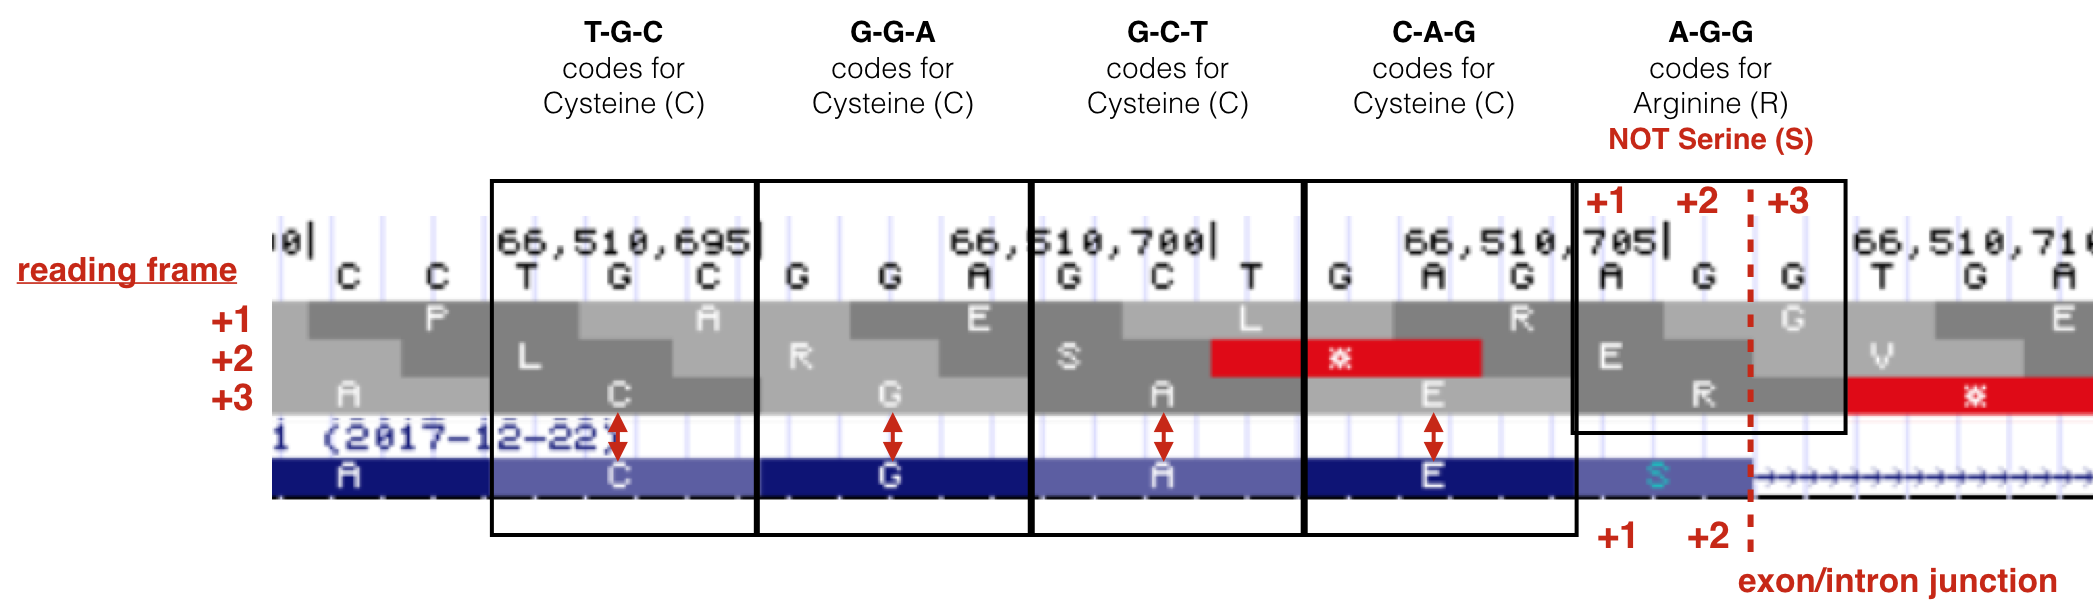
\includegraphics[width=0.75\linewidth]{static/images/splitcodon}

}

\caption{Modified from Lim and Burge 2001}\label{fig:codonsplit}
\end{figure}

\begin{figure}

{\centering 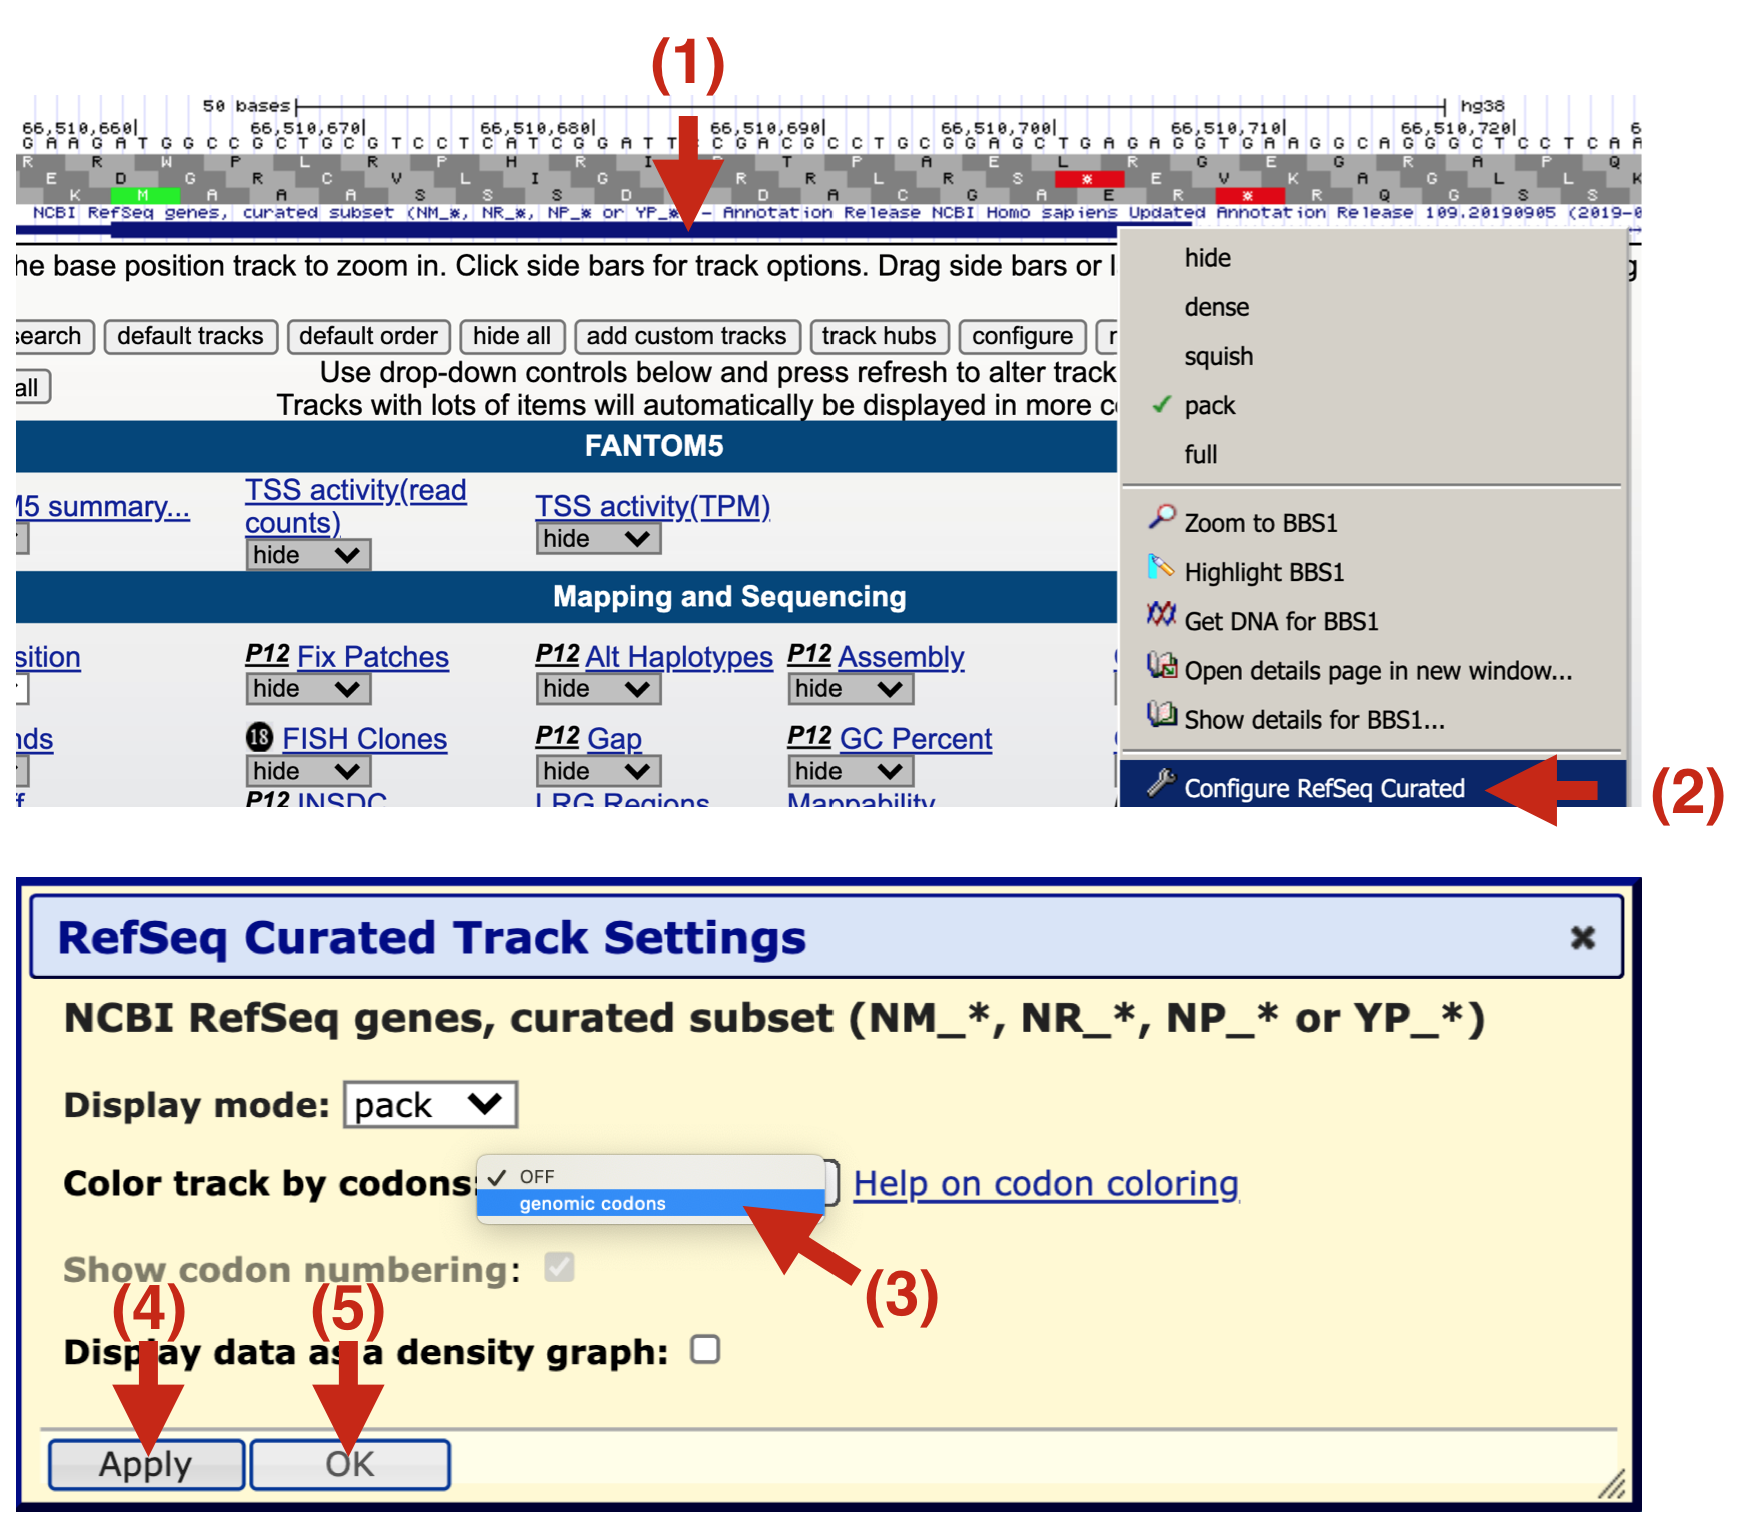
\includegraphics[width=0.75\linewidth]{static/images/colortrackon}

}

\caption{If your gene prediction track does not have the amino acids displayed (See 1 and compare to the figure above), then you will need to configure it anew as described here. 2) Right click on the gene prediction schematic and a pull down menu will appear. Choose 'Configure Refseq Curated'. 3) A new yellow box will appear. Click on the pulldown menu for Color track by codons and choose 'genomic codons'. 4) Click 'Apply' then 5) Click 'OK'}\label{fig:colortrack}
\end{figure}

\hypertarget{test-your-understanding-19}{%
\subsection{\texorpdfstring{\href{https://docs.google.com/forms/d/e/1FAIpQLSfHgaIissZpkT3FqjhWg-1wXB6vjbXZlTz9kqK_OFqTmUTNMw/viewform?usp=sf_link}{Test Your Understanding}}{Test Your Understanding}}\label{test-your-understanding-19}}

\begin{itemize}
\tightlist
\item
  \emph{The last codon in exon 1 of BBS1 is split by intron 1. This split codon normally codes for Serine (S). What is the sequence of this codon once splicing is complete?}
\item
  \emph{If splicing were to fail (intron 1 is not removed), what amino acid would be added after the ``E'' in the sequence C-G-A-E- at the end of exon 1?}
\item
  \emph{If splicing were to fail (intron 1 is not removed), how many amino acids would be added after the ``E'' before a stop codon is encountered? (NOTE: This is the same E as the one mentioned in the above question)}
\item
  \emph{The last codon in exon 2 of BBS1 is split by intron 2. This split codon normally codes for alanine. What is the sequence of this codon once splicing is complete?}
\item
  \emph{At what position is the last codon of exon 2 split by intron 2? The +1 or the +2?}
\item
  \emph{If splicing were to fail (intron 2 is not removed), what amino acid would be added after the ``L'' in the sequence S-A-C-L at end of exon 2?}
\item
  \emph{If splicing were to fail (intron 2 is not removed), how many amino acids would be added after the ``L'' before a stop codon is encountered? (NOTE: This is the same L as the one mentioned in the above question)}
\item
  \emph{Where is intron 3 of BBS1 positioned (at position +1 of a codon, at position +2 of a codon or between codons)?}
\item
  \emph{If splicing were to fail (intron 3 is not removed), how many incorrect amino acids would be added until a stop codon is encountered?}
\item
  \emph{Where is intron 7 of BBS1 positioned (at position +1 of a codon, at position +2 of a codon or between codons)?}
\item
  \emph{If splicing were to fail (intron 7 is not removed), how many incorrect amino acids would be added until a stop codon is encountered?}
\item
  \emph{Where is intron 9 of BBS1 positioned (at position +1 of a codon, at position +2 of a codon or between codons)?}
\item
  \emph{If splicing were to fail (intron 9 is not removed), how many incorrect amino acids would be added until a stop codon is encountered?}
\end{itemize}

In general, a codon can be split by an intron at any position: the +1 position, the +2 position or between codons. In Chapter 3, you learned that exons within a single gene can jump from one reading frame to another. The act of splicing brings these exons back into a \emph{single} reading frame. \emph{Thus, it is critical that splicing is accurate}. One mistake and the reading frame of an mRNA will get out of whack. The protein sequence will change and will most likely be shorter than normal. This explains why splice site mutations are often pathogenic in human disease genes. 86

\hypertarget{cleavage-and-polyadenylation}{%
\section{Cleavage and Polyadenylation}\label{cleavage-and-polyadenylation}}

Termination of transcription involves two coupled reactions: 1) \textbf{RNA cleavage} to release the RNA transcript from the RNA polymerase machinery and 2) \textbf{addition of a poly(A) tail}\footnote{polyadenylation} to the 3' end of the newly released message. Proper cleavage creates a transcript of the correct length. Addition of the poly A tail helps transport the mRNA out to the cytoplasm and improves stability and translation efficiency.

Like splicing, cleavage and polyadenylation requires specific RNA sequence motifs. These RNA motifs recruit the cleavage and polyadenylation machinery\footnote{a large multiprotein complex} to the RNA. Sequence motifs important for cleavage flank\footnote{are found on either side of} the cleavage site (Figure \ref{fig:cleavage}a). The best conserved motif is called the Poly A Site (or PAS), a sequence consisting of six ribonucleotides positioned 15-30 nucleotides upstream of the cleavage site \emph{within} the 3' UTR. A sequence logo of aligned PAS sequences from humans and flies illustrates this high level of conservation (Figure \ref{fig:cleavage}b) and reveals the consensus sequence as it would be found in the nontemplate strand of the genome\footnote{For a plus strand gene like BBS1, the nontemplate strand of the genome \emph{is} the plus strand}: AWTAAA (where W = T/A).

\begin{figure}

{\centering 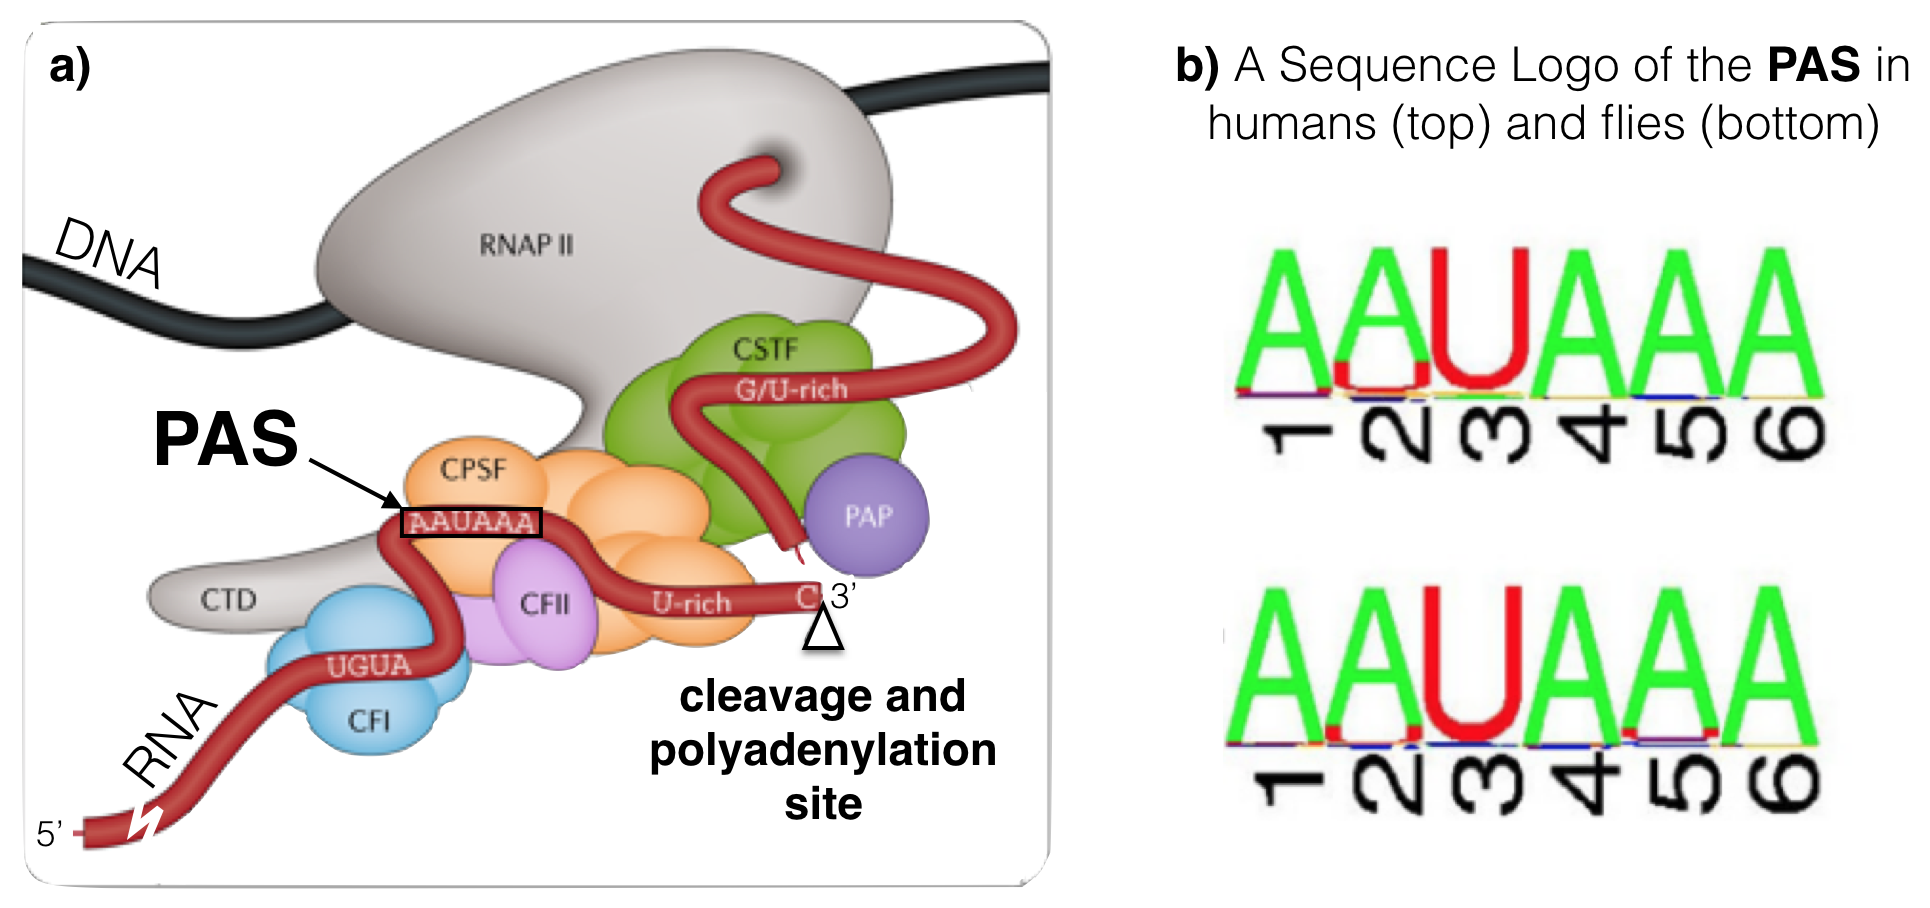
\includegraphics[width=1\linewidth]{static/images/PAS}

}

\caption{a) A schematic of an RNA (in red) just after cleavage but before polyadennylation. The 5' end of the RNA extends to the bottom left. An open triangle points to the site of cleavage. Notice that the PAS (AAUAAA) is upstream of the cleavage site. The G/U-rich region is downstream. CTD, CFI, CFII, CPSF, CSTF and PAP make up the cleavage and polyadenylation machinery. The **PAP** is the **P**oly **A** **P**olymerase, the enzyme that adds adenine ribonucleotides to the 3' end of the message. b) These sequence logos illustrate how conserved the PAS really is even between humans (top) and flies (bottom). }\label{fig:cleavage}
\end{figure}

\hypertarget{test-your-understanding-20}{%
\subsection{\texorpdfstring{\href{https://docs.google.com/forms/d/e/1FAIpQLSeLBjNg4Tjg5PpnU6SFMB9PcJzJvLEg6s9iwJKgzQR97Qtftw/viewform?usp=sf_link}{Test Your Understanding}}{Test Your Understanding}}\label{test-your-understanding-20}}

The following questions ask you to locate then describe the PAS for a variety of genes. To begin, open the \href{https://genome.ucsc.edu/s/megallegos/Biol\%20310\%20Module\%201}{``Gene structure''} session and use the Short Match evidence track to search for a PAS consensus sequence (AWTAAA).

\begin{itemize}
\tightlist
\item
  \emph{Search the 3' UTR of BBS1 for a PAS consensus sequence (AWTAAA). Write out your PAS sequence from 5' to 3' as it would be found in the nontemplate strand of the genome.}
\item
  \emph{How many nucleotides are there between the putative BBS1 PAS identified above and the cleavage site (for the putative position of cleavage, review the gene prediction evidence track).}
\item
  \emph{Is the putative BBS1 PAS upstream or downstream of the cleavage site?}
\item
  \emph{Is the putative BBS1 PAS located where it should be?}
\item
  \emph{Search the 3' UTR of ZDHHC24 (long isoform) for a PAS consensus sequence (AWTAAA). Don't forget! This is a minus strand gene nearby BBS1. Write out your PAS sequence from 5' to 3' as it would be found in the nontemplate strand of the genome.)}
\item
  \emph{How many nucleotides are there between the putative ZDHHC24 (long isoform) PAS and the cleavage site (for the position of cleavage, review the gene prediction evidence track).}
\item
  \emph{Is the putative ZDHHC24 (long isoform) PAS upstream or downstream of the cleavage site?}
\item
  \emph{Is the putative ZDHHC24 (long isoform) PAS located where it should be?}
\item
  \emph{Search the 3' UTR of ZDHHC24 (short isoform) for a PAS consensus sequence (AWTAAA). Write out your PAS sequence from 5' to 3' as it would be found in the nontemplate strand of the genome.)}
\item
  \emph{How many nucleotides are there between the putative ZDHHC24 (short isoform) PAS and the cleavage site (for the position of cleavage, review the gene prediction evidence track).}
\item
  \emph{Is the putative ZDHHC24 (short isoform) PAS upstream or downstream of the cleavage site?}
\item
  \emph{Is the putative ZDHHC24 (short isoform) PAS located where it should be?}
\item
  \emph{Find the MYH3 gene and check which strand it is on. Then search the 3' UTR of MYH3 for a PAS consensus sequence (AWTAAA). Write out your PAS sequence from 5' to 3' as it would be found in the nontemplate strand of the genome.)}
\item
  \emph{How many nucleotides are there between the putative MYH3 PAS and the cleavage site (for the position of cleavage, review the gene prediction evidence track).}
\item
  \emph{Is the putative MYH3 PAS upstream or downstream of the cleavage site?}
\item
  \emph{Is the putative MYH3 PAS located where it should be?}
\end{itemize}

Take home message: Splicing, cleavage and polyadenlyation are distinct from cap addition. The capping enzyme does not require a specific DNA or RNA sequence for 5' cap addition to occur. On the other hand, splicing, cleavage and polyadenylation do require specific sequence motifs. These sequences are present in the \textbf{nontemplate} or \textbf{sense} strand of the genome\footnote{For a plus strand gene, like BBS1, the nontemplate or sense strand is the plus strand.} but are recognized by the RNA processing machinery as RNA.

\hypertarget{translation-initiation}{%
\section{Translation Initiation}\label{translation-initiation}}

Once processed, mRNA exits the nucleus to be used as a template to create a polypeptide via a process called \textbf{translation}. Translation is mediated in part by the ribosome\footnote{The ribosome is comprised of two large complexes (one large and one small) made up of protein and RNA. Translation also requires tRNAs and of course, amino acids!}. In eukaryotes, the small ribosomal subunit and associated factors first assemble at the mRNA cap structure then scan along the 5' UTR until a start codon is found. Choosing the correct start codon is critical as it determines the reading frame and thus the polypeptide sequence! During the scanning process, ribosomal proteins within the small ribosomal subunit search for then interact with specific nucleotides both upstream and downstream of the start codon (Llacer et al.~2018). \textbf{In other words, context matters.}

The importance of context in start codon selection by the ribosome was first suggested by Marilyn Kozak. She aligned 699 well-characterized start codons derived from a set of vertebrate genes to search for sequence conservation upstream and downstream of the ATG (Kozak 1987). She then converted this large multiple sequence alignment into a nucleotide frequency table\footnote{Sequence logos were not ``invented'' until 1990 by Schneider and Stephens} (Figure \ref{fig:humankozak}A). The most frequent nucleotides she found at each position from -6 to +4 is called the Kozak consensus sequence: GCCACC\textbf{ATG}G.

Now we have sequence for entire genomes! In 2015, Cenik et al.~created a sequence logo for a similar region surrounding the start codon for all protein coding genes in the human genome (Figure \ref{fig:humankozak}B). The results are surprisingly similar. Again, the fact that sequence conservation exists suggests that the sequence surrounding the ATG plays an important role in translation initiation.

\begin{figure}

{\centering 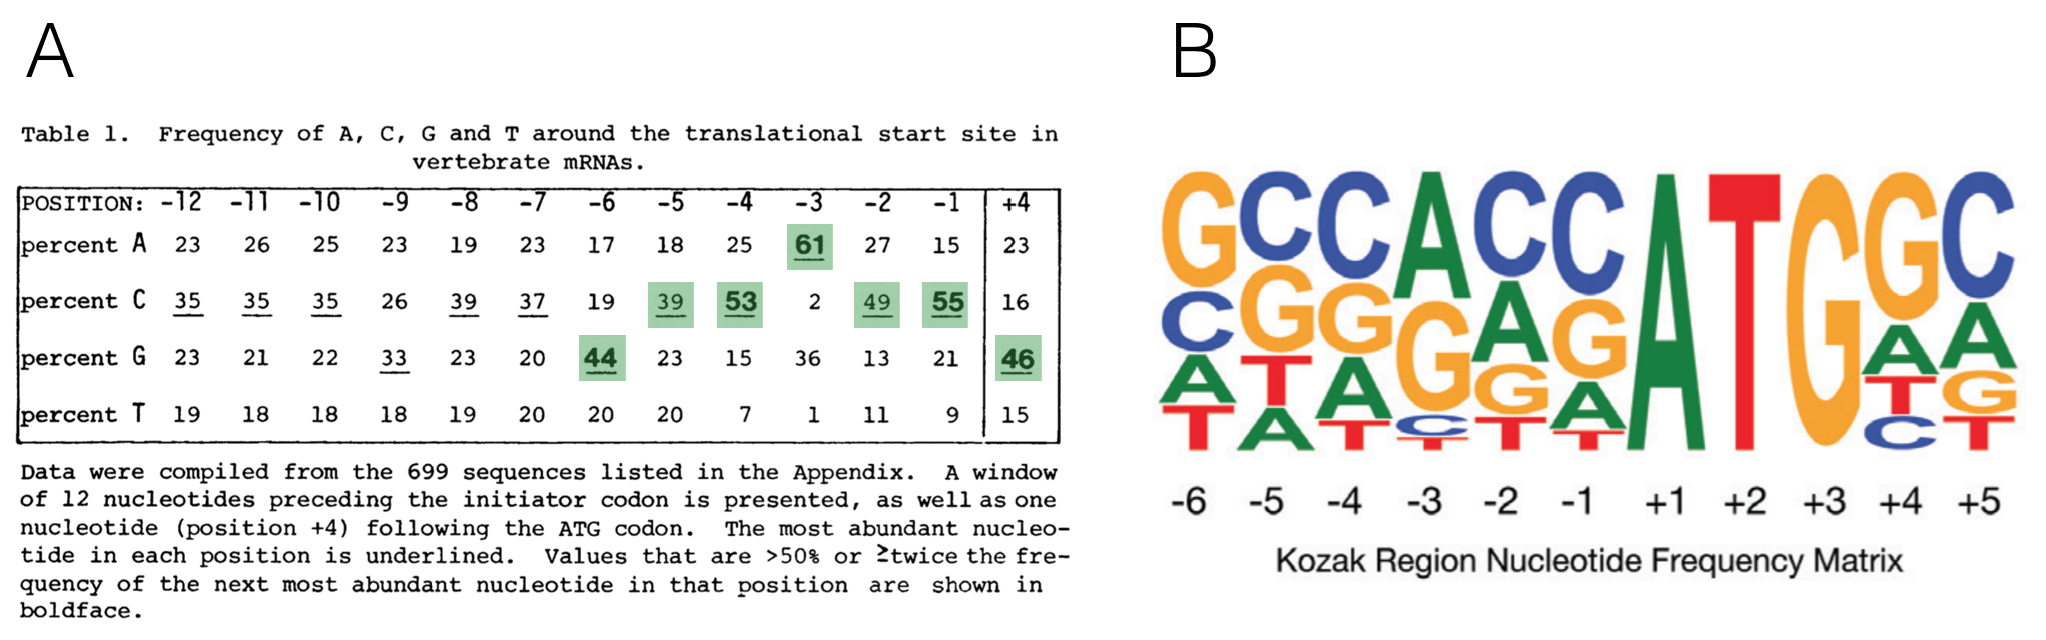
\includegraphics[width=1\linewidth]{static/images/humanseqlogo}

}

\caption{A) A multiple sequence alignment of 699 vertebrate genes displayed as a nucleotide frequency table (The ATG is not included since it is invariant). This schematic is from Kozak, 1987 with the most frequently observed nucleotides at positions -6 to +4 highlighted in green. B) This sequence logo was created 28 yeats later from the complete set of human protein coding genes. Notice the similarities!}\label{fig:humankozak}
\end{figure}

A recent study in zebrafish supports this hypothesis. In this study, Grzegorski et al.~inserted the Kozak consensus sequence (GCCACC\textbf{ATG}G) into a reporter gene\footnote{In molecular biology, reporter genes are those that can easily be visualized by eye when translated into protein. For example, lacZ is a good reporter because its gene product, B-galactosidase, turns one of its substrates blue. Importantly, there is a linear relationship between the amount of blue pigment produced and the amount of B-galactosidase produced. GFP is also a good reporter which can be visualized by fluorescence microscopy. Reporter genes are used for a large variety of purposes but in this study it was used to measure translation efficiency} then measured the efficiency of translation by visualizing the amound of reporter gene product made. This was the control. They then compared the expression of this control reporter gene to ones with other translation initiation sequences (i.e.~GCAAAC\textbf{ATG}G, GCAGTC\textbf{ATG}G, CTTTCT\textbf{ATG}C or CGGTGT\textbf{ATG}C). They discovered that a reporter gene fused to a translational initiation sequence found \emph{less frequently} in the genome than the canonical Kozak consensus sequence (GCCACC\textbf{ATG}G) was translated to lower levels than the control. By contrast, a reporter gene containing a translational initiation sequence found \emph{more frequently} in the genome than the Kozak consensus was translated to higher levels than the control. Their results are shown in Figure \ref{fig:startcodonreporter}.

\begin{figure}

{\centering 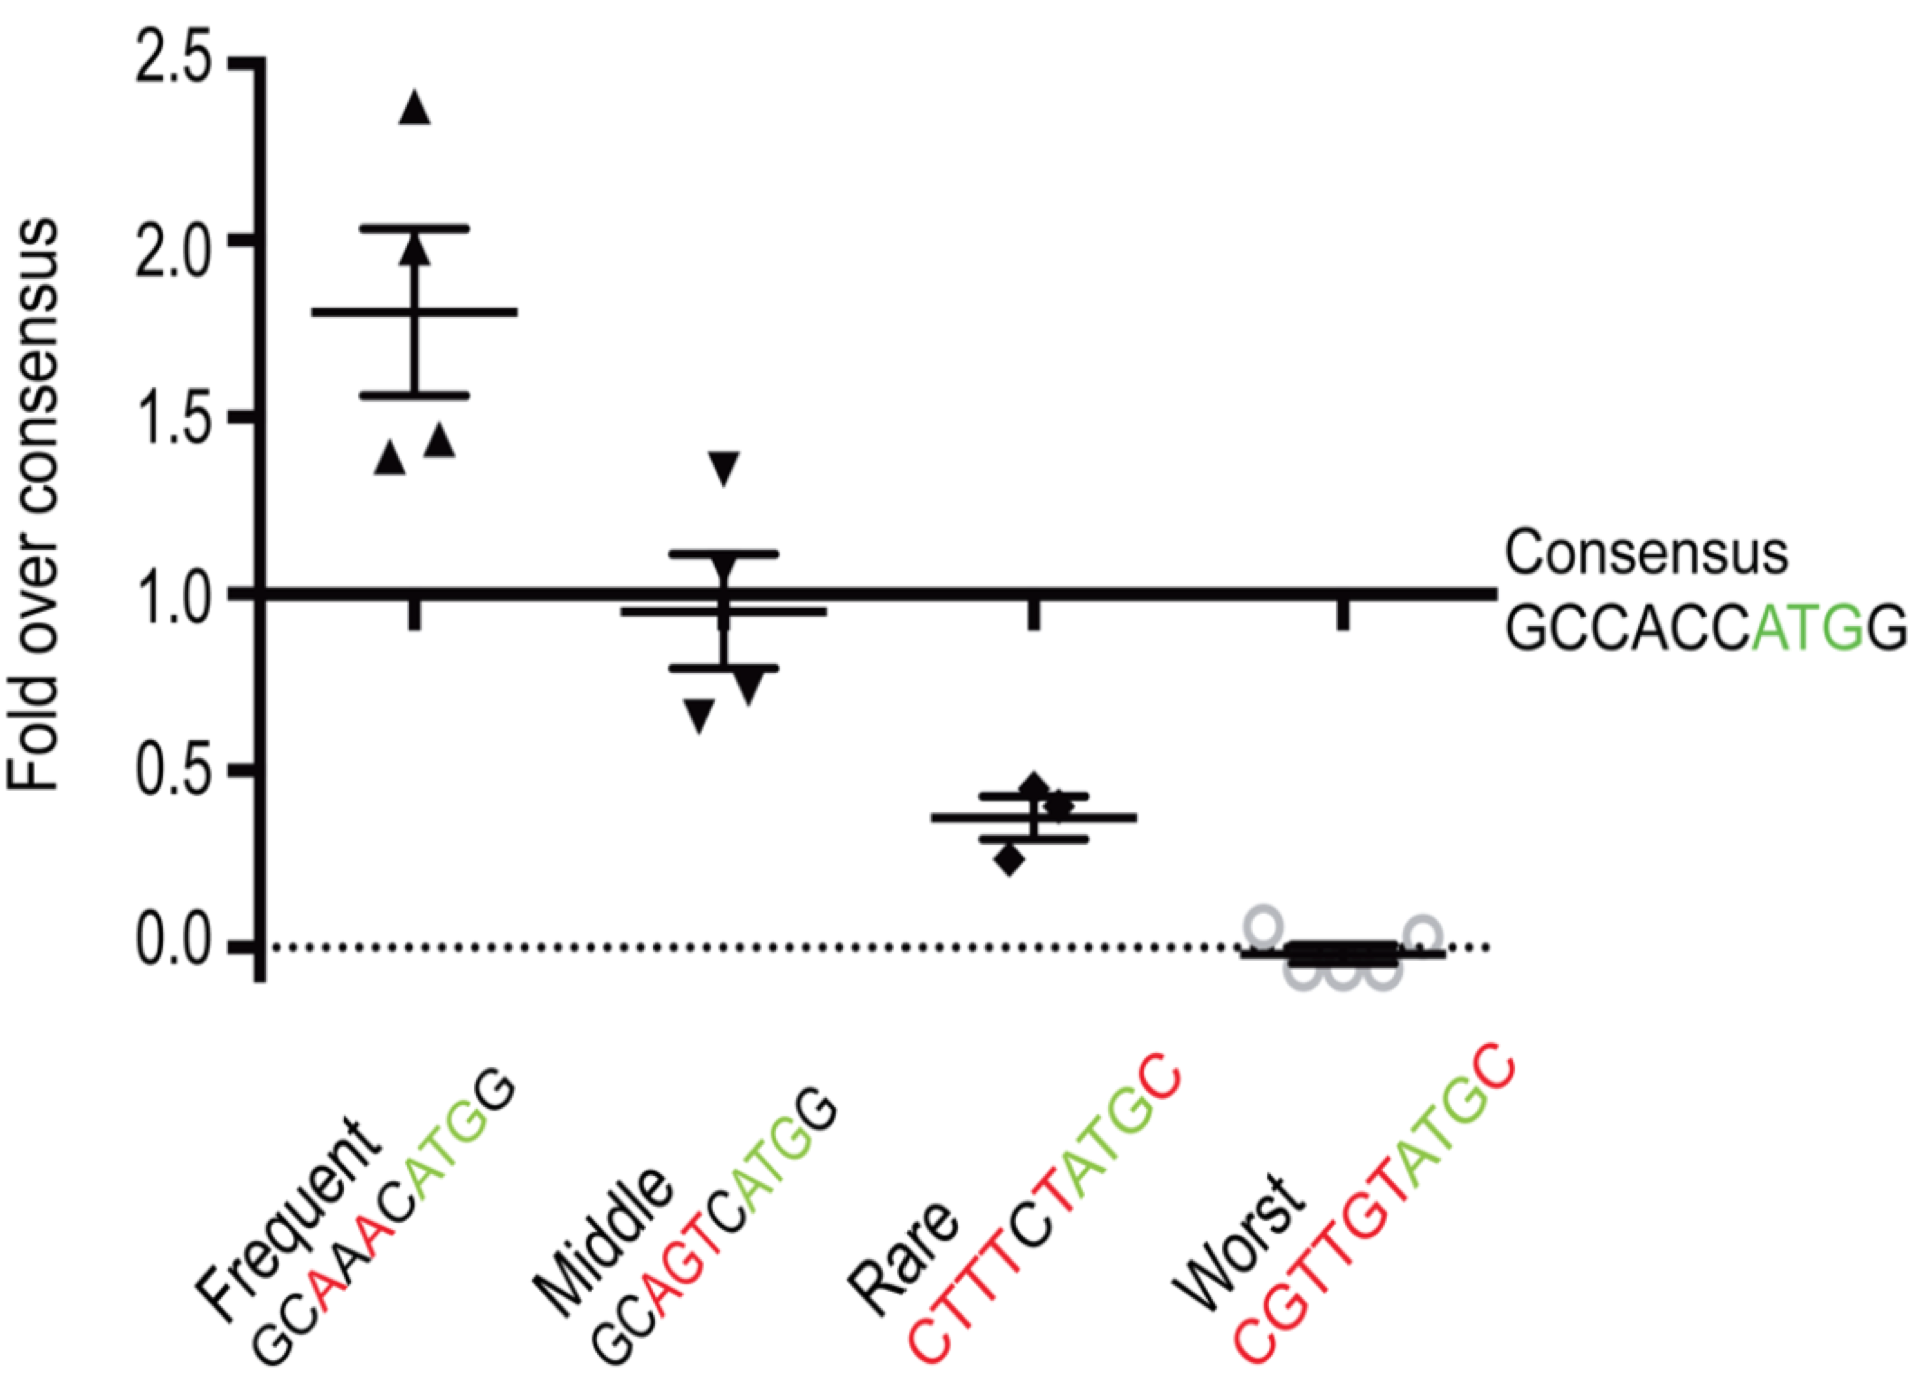
\includegraphics[width=0.5\linewidth]{static/images/ATGreporter}

}

\caption{Figure taken from Grzegorski et al. 2014. The Y-axis represents expression levels of the experimental reporter gene divided by expression levels of the control reporter gene containing the canonical kozak consensus sequence }\label{fig:startcodonreporter}
\end{figure}

Additional studies found that nucleotides in two highly conserved positions exert the strongest effect: a G residue following the ATG codon (position +4) and a purine three nucleotides upstream (position -3). Thus, overall, a good start codon is one found in the following context: RNNATGG (Where R is a purine and N is any nucleotide). Whereas an adequate start codon is RNNATGY or YNNATGG (where Y is a pyrimidine) (Kozak 1997).

\hypertarget{test-your-understanding-21}{%
\subsection{\texorpdfstring{\href{https://docs.google.com/forms/d/e/1FAIpQLSdUb7zLFClMM3JsMUwTKL2YQxSfFQnefExu2x7GsDg02Tz0WQ/viewform?usp=sf_link}{Test Your Understanding}}{Test Your Understanding}}\label{test-your-understanding-21}}

The following questions ask you to evaluate the predicted start codon for a variety of genes. To identify the predicted start codon, review the gene prediction track.

\begin{itemize}
\tightlist
\item
  \emph{Is the predicted BBS1 start codon found in a good context (RNN\textbf{ATG}G), adequate context (RNN\textbf{ATG}Y or YNN\textbf{ATG}G) or neither?}
\item
  \emph{Now, find the DPP3 gene just upstream of BBS1. Is the predicted DPP3 start codon found in a good context (RNN\textbf{ATG}G), adequate context (RNN\textbf{ATG}Y or YNN\textbf{ATG}G) or neither?}
\item
  \emph{Now, find the ZDHHC24 gene just downstream of BBS1. Is the predicted ZDHHC24 start codon found in a good context (RNN\textbf{ATG}G), adequate context (RNN\textbf{ATG}Y or YNN\textbf{ATG}G) or neither?}
\item
  \emph{Now, find the MYH3 gene (use the search window). Is the predicted MYH3 start codon found in a good context (RNN\textbf{ATG}G), adequate context (RNN\textbf{ATG}Y or YNN\textbf{ATG}G) or neither?}
\end{itemize}

\hypertarget{uorfs}{%
\section{uORFs}\label{uorfs}}

uORF stands for upstream Open Reading Frame (pronounced you-orf). A gene is said to have a uORF if it has a start codon in the putative 5' UTR followed by an \textbf{in-frame} stop codon that precedes the \textbf{end} of the main coding sequence or so-called primary ORF (Figure \ref{fig:uORFdefined}).

\begin{figure}

{\centering 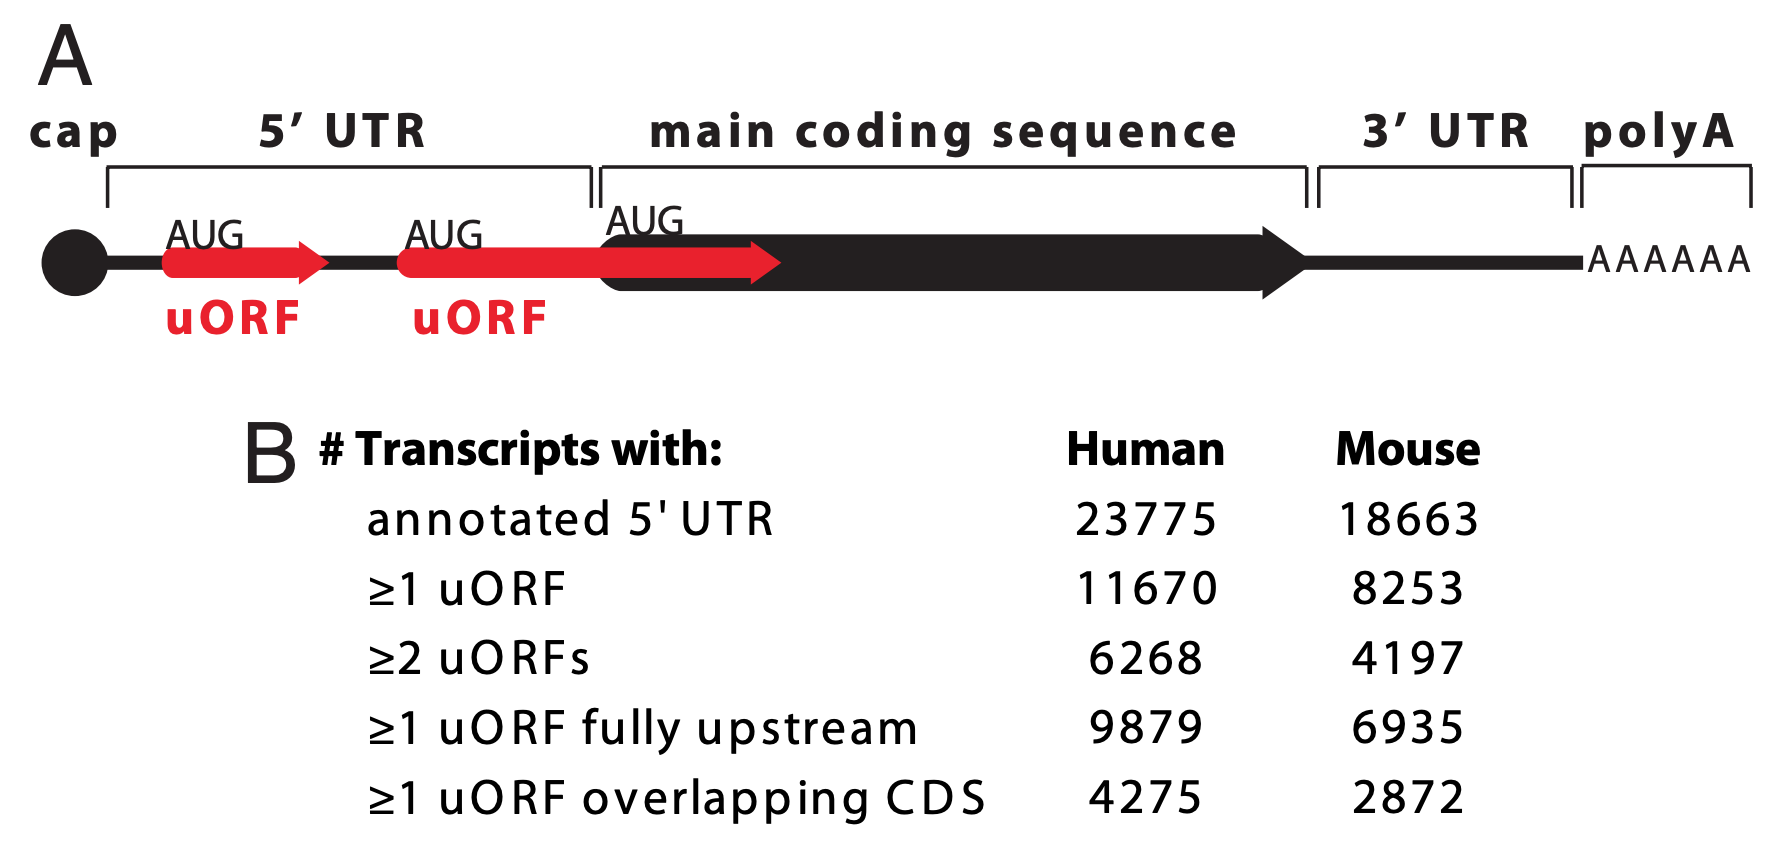
\includegraphics[width=0.7\linewidth]{static/images/uORFdefinition}

}

\caption{Paraphrased from Calvo et al. 2009. A) A schematic representation of an mRNA transcript with two uORFs (red arrows), one fully upstream and one overlapping the main coding sequence (black arrow). uORFs were defined by Calvo et al. as a start codon (AUG) in the 5' UTR followed by an in-frame stop codon (arrowhead) that precedes the **end** of the main coding sequence. Calvo et al. 2009 further refines the definition to only include uORFs that code for a minimum peptide length of 3 amino acids (or a coding sequence minimum length of 9 nt). (B) Number of uORFs in human and mouse RefSeq transcripts.}\label{fig:uORFdefined}
\end{figure}

uORFs, in general, have the capacity to reduce translation initiation from the bonafide start codon (Calvo et al.~2009). Since they are found in a large number of protein coding genes (nearly 50\% of human genes are thought to have a uORF), this is thought to be ``by design''. In other words, it is thought that the presence of a uORF has an important purpose and is subject to positive selection during evolution as a way to keep gene expression levels appropriately low. Two examples are described in Figure \ref{fig:uORFregulation}.

\begin{figure}

{\centering 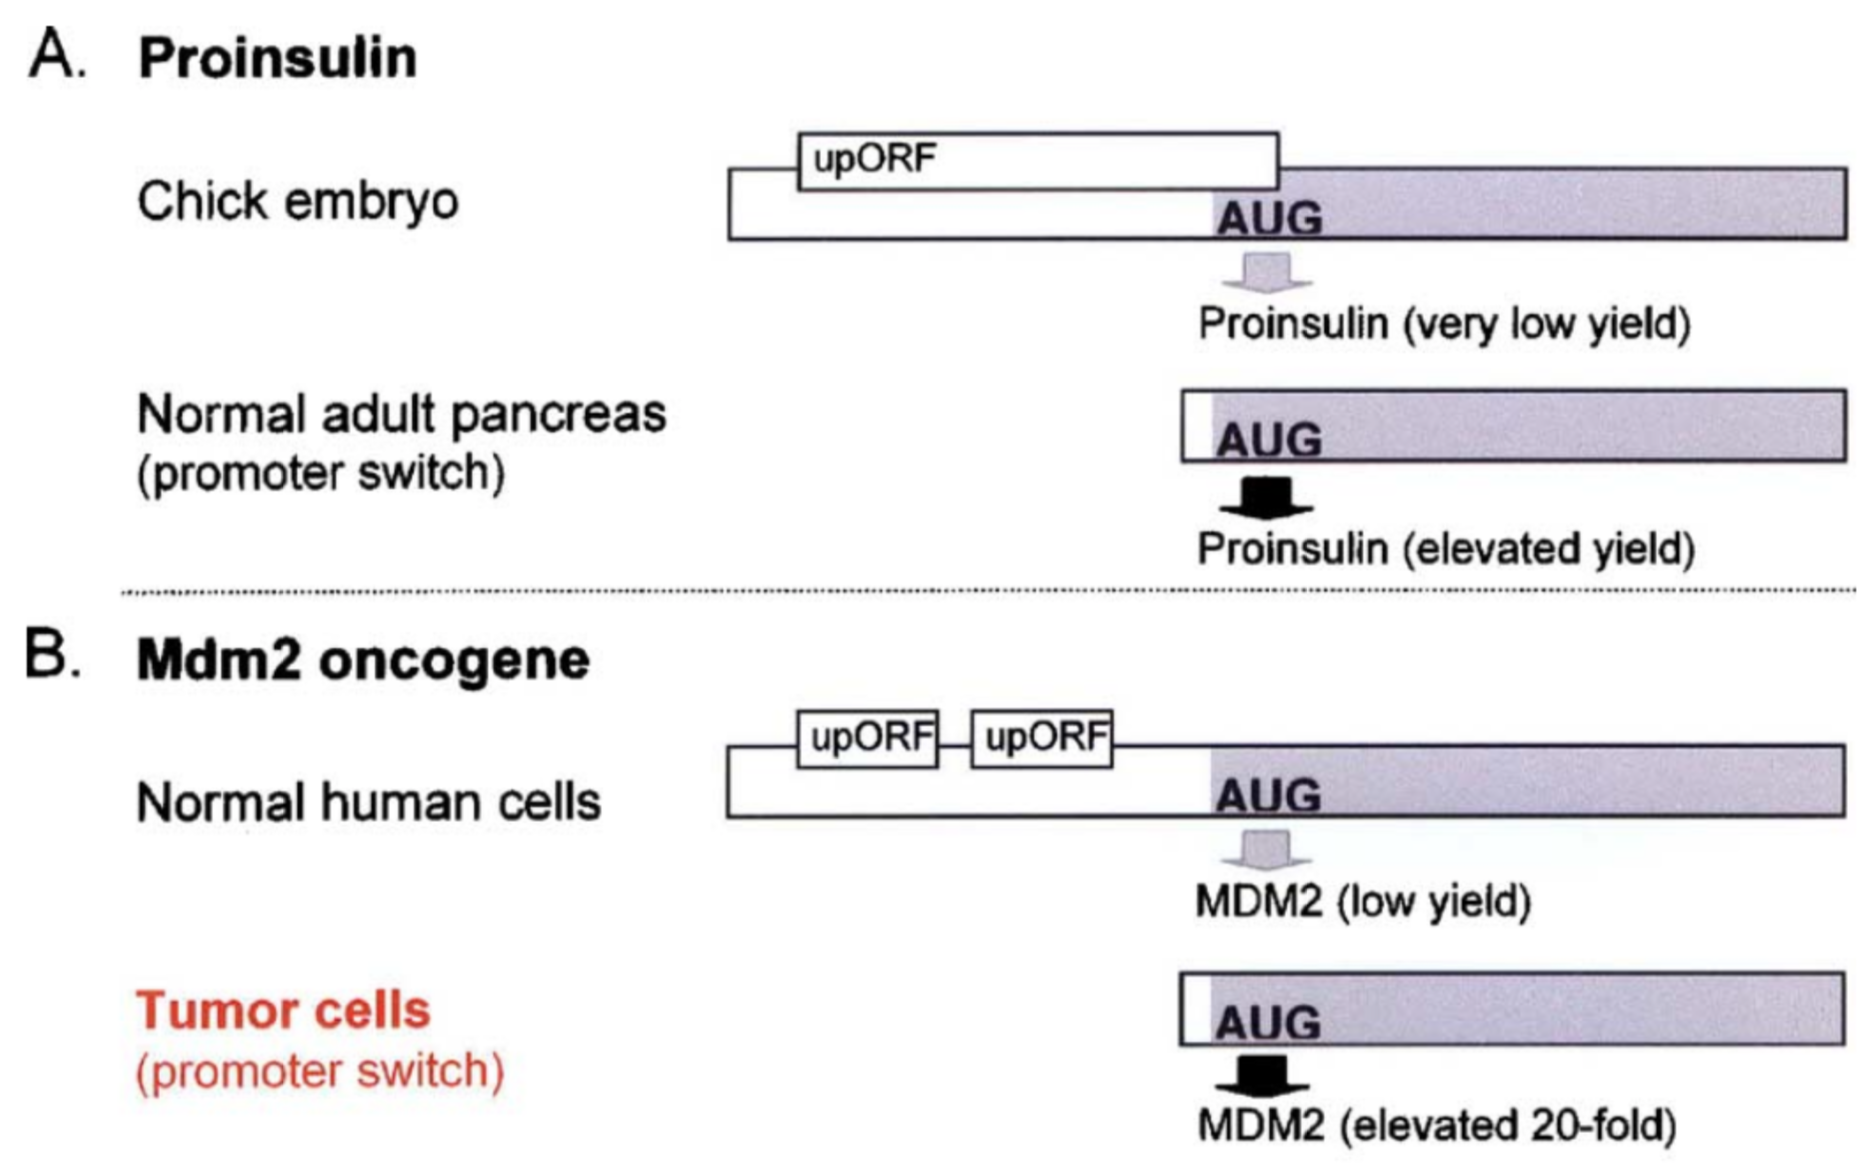
\includegraphics[width=0.7\linewidth]{static/images/uORFexamples}

}

\caption{Paraphrased from Kozak, 2005. Small upstream ORFs or uORFs are thought to down-regulate translation by imposing an inefficient reinitiation mechanism. This constraint on translation ensures against harmful overproduction of potent or toxic proteins. Two examples are described here. A) The presence of an overlapping uORF allows only low-level production of proinsulin in chick embryos. In the adult pancreas where more proinsulin protein is needed, a more efficiently translated form of mRNA is produced via a downstream promoter. B) The human mdm2 oncogene has the ability to cause cancer when it is overexpressed. Overexpression of the mdm2 oncogene in tumor cells is caused by a switch in the transcriptional start site which eliminates two small uORFs, thereby elevating translation 20-fold. The first example illustrates a naturally occuring, developmental switch in gene expression. The second example only occurs in the disease state. In fact, the expression from the crytpic downstream promoter results from the presence of a p53-responsive promoter region that is preferentially utilized when p53 levels increase, a common occurance in tumor cells (Landers 1997)}\label{fig:uORFregulation}
\end{figure}

\hypertarget{recognizing-uorfs}{%
\section{Recognizing uORFs}\label{recognizing-uorfs}}

To determine if a gene of interest (GOI) has a uORF in its 5' UTR, you need to focus your genome browser on the 5' UTR of your GOI then make sure your base prediction track is set to full. So long as you are zoomed in close enough to see the green boxes (start codons) and red boxes (stop codons) in the three reading frames, you can recognize uORFs. For an example of what a uORF would look like, see Figure \ref{fig:MDM2uORF}. At some point you may come across a gene with an intron in the 5' UTR (it's rare). Just keep in mind that these 5' UTRs are more difficult to assess because the uORF may switch reading frames if it spans the intron.

\begin{figure}

{\centering 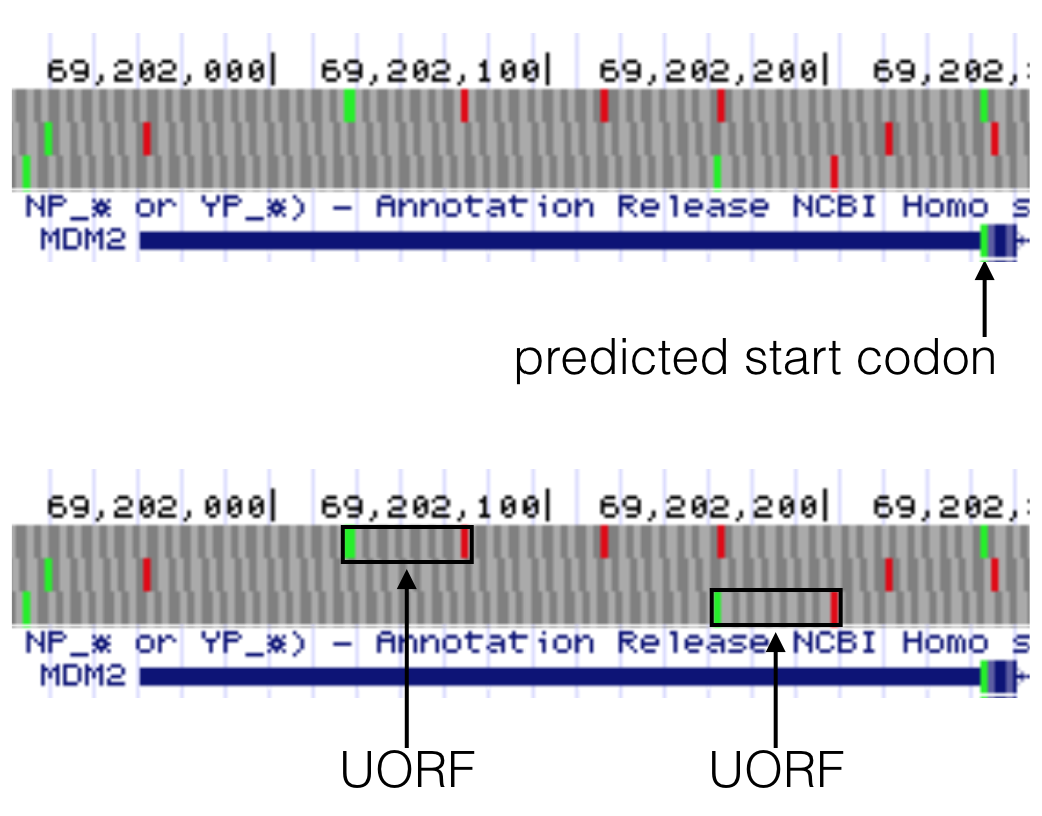
\includegraphics[width=0.5\linewidth]{static/images/Recognizing_uORFs}

}

\caption{MDM2 has two uORFs in the 5' UTR as highlighted here in the bottom image. Both uORFs by definition are upstream of the predicted start codon as highlighted in the top image. Notice a uORF is defined as a start codon in the 5' UTR that is followed by a stop codon **in the same reading frame**.}\label{fig:MDM2uORF}
\end{figure}

\hypertarget{test-your-understanding-22}{%
\subsection{\texorpdfstring{\href{https://docs.google.com/forms/d/e/1FAIpQLSe-oas9GK1E-KqyOOzGnrdZGzwiY6GRGVgwlce4FB7GHzW1zg/viewform?usp=sf_link}{Test Your Understanding}}{Test Your Understanding}}\label{test-your-understanding-22}}

\begin{itemize}
\tightlist
\item
  \emph{Does BBS1 have a uORF in the 5' UTR?}
\item
  \emph{If yes, is the uORF found in a good context (RNN\textbf{ATG}G), adequate context (RNN\textbf{ATG}Y or YNN\textbf{ATG}G) or neither?}
\item
  \emph{Search for the gene, TAS2R3. It has a uORF in its 5' UTR that is known to impact translation of the primary ORF (Calvo et al.~2009). Is the ATG of the uORF found in a good context (RNN\textbf{ATG}G), adequate context (RNN\textbf{ATG}Y or YNN\textbf{ATG}G) or neither?}
\item
  \emph{Search for the gene, SFXN3. It has a uORF in its 5' UTR that is known to impact translation of the primary ORF (Calvo et al.~2009). Is the ATG of the uORF found in a good context (RNN\textbf{ATG}G), adequate context (RNN\textbf{ATG}Y or YNN\textbf{ATG}G) or neither?}
\item
  \emph{Search for the gene, ADH5. It has a uORF in its 5' UTR that is known to impact translation of the primary ORF (Calvo et al.~2009). There are two start codons in-frame with a downstream stop codon within the 5' UTR. Evaluate the context of these two start codons to determine if these start codons are found in a good context (RNN\textbf{ATG}G), adequate context (RNN\textbf{ATG}Y or YNN\textbf{ATG}G) or neither.}
\item
  \emph{Search for the gene, UCP2. It has a uORF in its 5' UTR that is known to impact translation of the primary ORF (Calvo et al.~2009). There are three start codons in frame with a downstream stop codon. Evaluate the context of these three start codons to determine if these start codons are found in a good context (RNN\textbf{ATG}G), adequate context (RNN\textbf{ATG}Y or YNN\textbf{ATG}G) or neither.}
\end{itemize}

\hypertarget{for-discussion-3}{%
\section{\texorpdfstring{\href{https://docs.google.com/forms/d/e/1FAIpQLScUUIanAotTGMtaVZY51ZcYjrJF1qkbuy08SwycPIQrdn8raA/viewform?usp=sf_link}{For Discussion}}{For Discussion}}\label{for-discussion-3}}

\begin{enumerate}
\def\labelenumi{\arabic{enumi}.}
\tightlist
\item
  How did you go about identifying a uORF when you answered your ``Test Your Understanding'' questions above?
\end{enumerate}

\hypertarget{homework}{%
\section{Homework}\label{homework}}

Create your own consensus sequence and sequence logo.

\textbf{If the first letter of your last name falls within A-M:}

Part 1. Click the appropriate link to download a \href{https://drive.google.com/file/d/1d0c37m7lQloME0VEw_z_fILAdVX7DrgH/view?usp=sharing}{DOCX file} or a \href{https://drive.google.com/file/d/1NPnzu2LG8kIRGlXKBQVJdWZG3PSGzKvs/view?usp=sharing}{PDF file}. Complete the \textbf{left side} of the table (Figure \ref{fig:intronMSA}). Instructions are included in the file. Review Figure \ref{fig:BBS1transcript} to remind yourself what an intron looks like and Figure \ref{fig:exonjumpingtips} to see how I completed the second row of the table.
Part 2. Create a \textbf{sequence logo} for the multiple sequence alignment you built using the \href{https://weblogo.berkeley.edu/logo.cgi}{web logo} website. See (Figure \ref{fig:weblogopage}) for instructions on how to use the weblogo site.

\textbf{If the first letter of your last name falls within N-Z:}

Part 1. Click the appropriate link to download a \href{https://drive.google.com/file/d/1d0c37m7lQloME0VEw_z_fILAdVX7DrgH/view?usp=sharing}{DOCX file} or a \href{https://drive.google.com/file/d/1NPnzu2LG8kIRGlXKBQVJdWZG3PSGzKvs/view?usp=sharing}{PDF file}. Complete the \textbf{right side} of the table (Figure \ref{fig:intronMSA}). Instructions are included in the file. Review Figure \ref{fig:BBS1transcript} to remind yourself what an intron looks like and Figure \ref{fig:exonjumpingtips} to see how I completed the second row of the table.
Part 2. Create a \textbf{sequence logo} for the multiple sequence alignment you built using the \href{https://weblogo.berkeley.edu/logo.cgi}{web logo} website. See (Figure \ref{fig:weblogopage}) for instructions on how to use the weblogo site.

DM your files directly to your instructor via SLACK.

\begin{figure}

{\centering 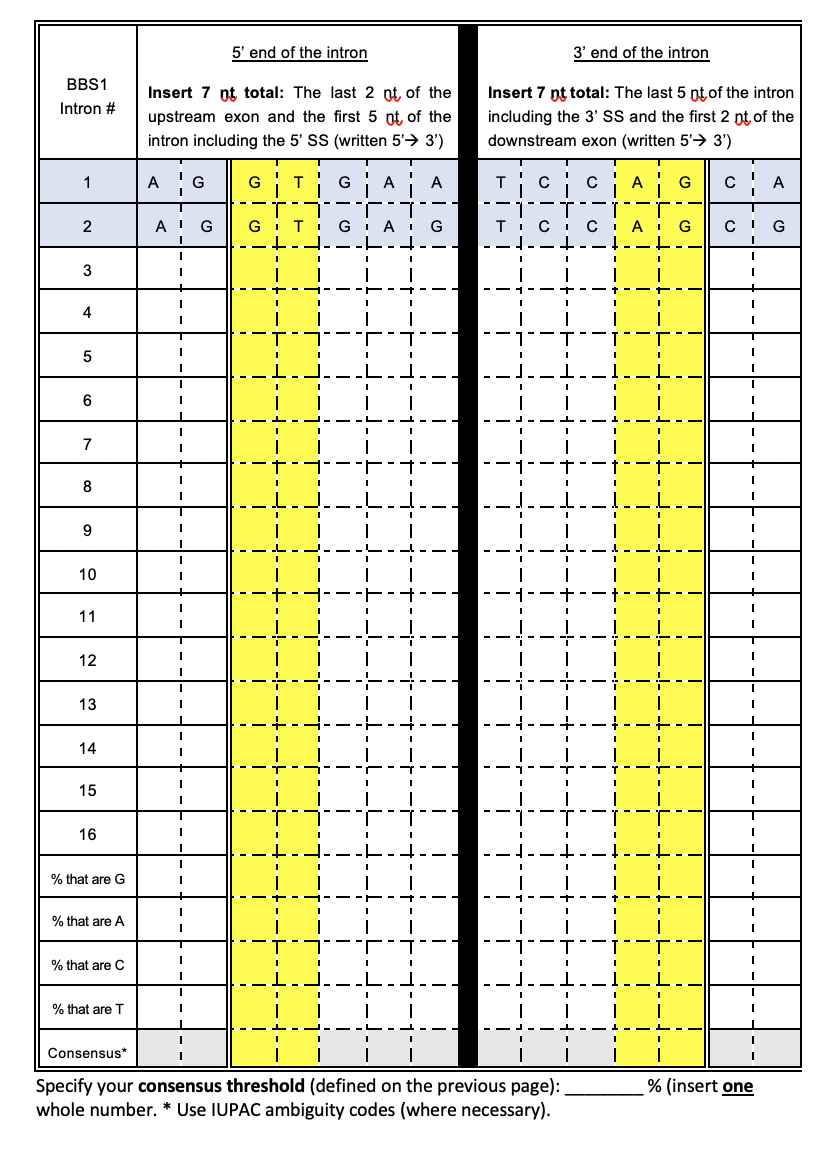
\includegraphics[width=0.5\linewidth]{static/images/IntronMSAhomework}

}

\caption{Complete either the left half or right half of the table (depending on the first letter of your last name - see below for more detailed instructions). The first two rows have been completed for you. Make sure you understand where this sequence comes from. The columns highlighted in yellow correspond to the 5' splice site (left half) or 3' splice site (right half). Links to the assignment can be found below.}\label{fig:intronMSA}
\end{figure}

\begin{figure}

{\centering 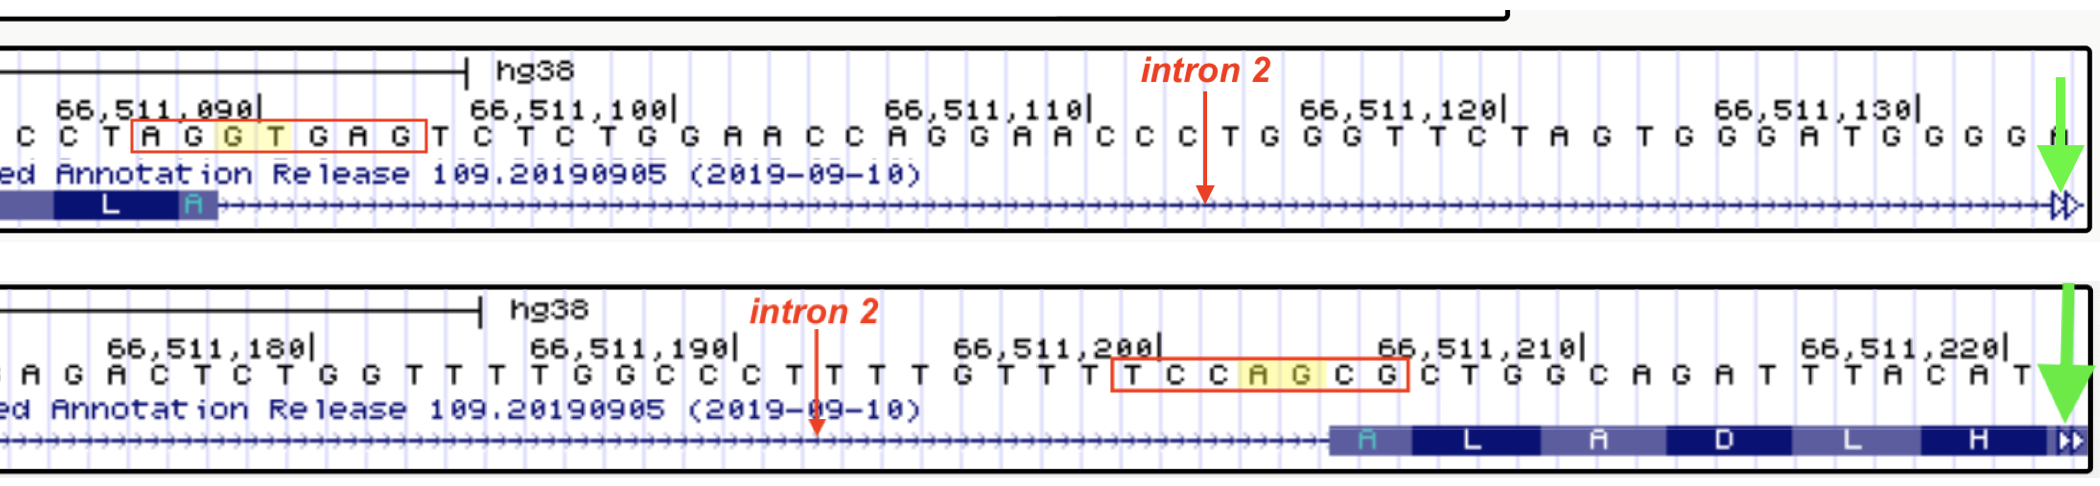
\includegraphics[width=1\linewidth]{static/images/5primeSS}

}

\caption{The exon-intron junctions of intron two are shown here. The sequences boxed in red outline the sequence that were input into row 2 of the table above. The top image includes the 5' end of intron 2. The bottom image includes the 3' end of intron 2. The 5' (top) and 3' (botom) splice sites are highlighted in yellow. To quickly jump to the next intron-exon junction, click on the open arrowhead on the far right (green arrows point to the open arrowheads). Another way to quickly view 5’ and 3’ splice site sequences is by clicking on the gene schematic in the NCBI Refseq track and then by clicking on the 'View details of parts of alignment within browser window' link.}\label{fig:exonjumpingtips}
\end{figure}

\begin{figure}

{\centering 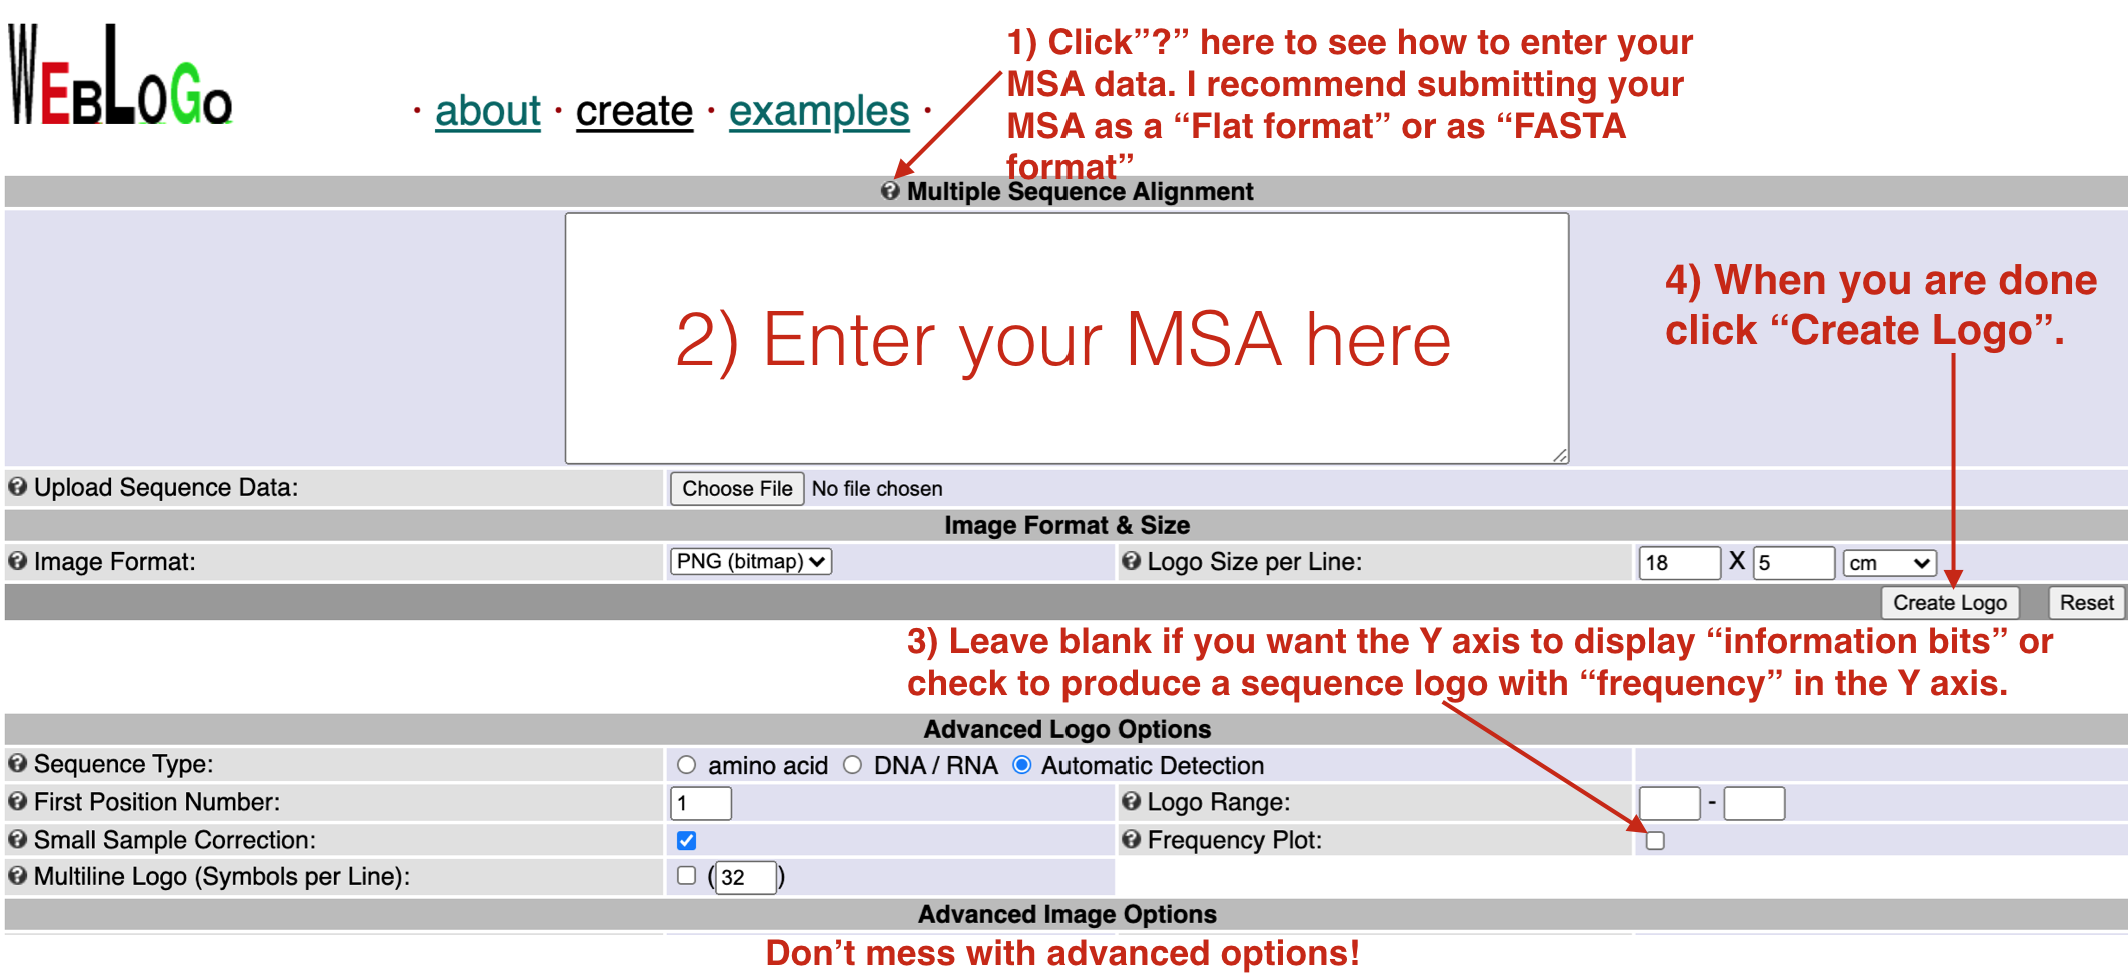
\includegraphics[width=1\linewidth]{static/images/weblogoInstructions}

}

\caption{To use the Weblogo site successfully, follow the instructions as outlined above.}\label{fig:weblogopage}
\end{figure}

© 2019, Maria Gallegos. All rights reserved.

\hypertarget{gene-discovery-using-pathogenic-sequence-variants}{%
\chapter{Gene discovery using pathogenic sequence variants}\label{gene-discovery-using-pathogenic-sequence-variants}}

A \textbf{Sequence variant}\footnote{Everyone's genome contains millions of sequence variants (small differences in sequence), that make each person unique. Most variants have unknown effects. Some contribute to differences between humans like eye color and blood type while a small number cause disease. Common variants are often described as single-nucleotide polymorphisms (SNPs) while rare variants that lead to disease are sometimes called mutations. That said, it does not make sense to use the word ``mutant'' when humans are discussed. This word is typically reserved for genetic model systems or laboratory animals that are known to be inbred} that leads to disease (or any measurable change in an organism's phenotype) provides evidence for the existence of a gene. When a sequence variant is mapped to the genome, the location of the gene is also discovered.

To follow along with the text and to answer ``Test Your Understanding'' questions, you will be using the \href{https://genome.ucsc.edu/s/megallegos/Biol\%20310\%3A\%20Module\%204\%3A\%20Mutational\%20Analysis}{``Sequence Variants''} session for this chapter.

\hypertarget{one-gene-two-definitions}{%
\section{One Gene: Two Definitions}\label{one-gene-two-definitions}}

A gene can be defined as a segment of DNA that is transcribed. To prove a gene exists using this definition, one can search for physical evidence: the gene product itself. In chapters four and five, we looked at RNA as physical evidence. A gene is also defined as ``a \emph{functional} unit of inheritance''. To prove a gene exists using this definition one can look for a phenotypic change that is passed from one generation to the next. Heritable phenotypic changes are caused by sequence variants that fall \emph{within genes}. Thus, a sequence variant that causes a phenotypic change can be used as physical evidence, pinpointing the location of a gene.

That said, \emph{every} gene cannot be identified in this way even if a DNA variant renders a gene inactive. Why? Some genes when inactive do not produce a measurable phenotypic change. Why you ask? Perhaps you don't know where to look or what to measure. Or there might be more than one gene with the same function (genetic redundancy\footnote{In engineering the word redundancy is used to describe the inclusion of extra components which are not strictly necessary to functioning, but are there in case of failure of other components. In genetics, genetic redundancy is a term used to describe situations where a given biochemical function is encoded by two or more genes that perform the same function. In these cases, mutations (or defects) in one of these genes will have a smaller effect on the fitness of the organism than expected from the genes' known function. Paraphrased from Wikipedia}) and thus inactivating one gene may not lead to a phenotypic change because another similar gene is still functional.

\hypertarget{understanding-dna-variants}{%
\section{Understanding DNA variants}\label{understanding-dna-variants}}

Open the \href{https://genome.ucsc.edu/s/megallegos/Biol\%20310\%3A\%20Module\%204\%3A\%20Mutational\%20Analysis}{``Sequence Variants''} session to view DNA variants that map to BBS1. Each variant is colored according to its known clinical significance: red for pathogenic, green for benign and gray for uncertain significance. Each mutation is also coded according to type (i.e.~substitution or InDel). See (Figure \ref{fig:MutationCodes}) for a list of DNA variant codes you are likely to encounter.

\begin{figure}

{\centering 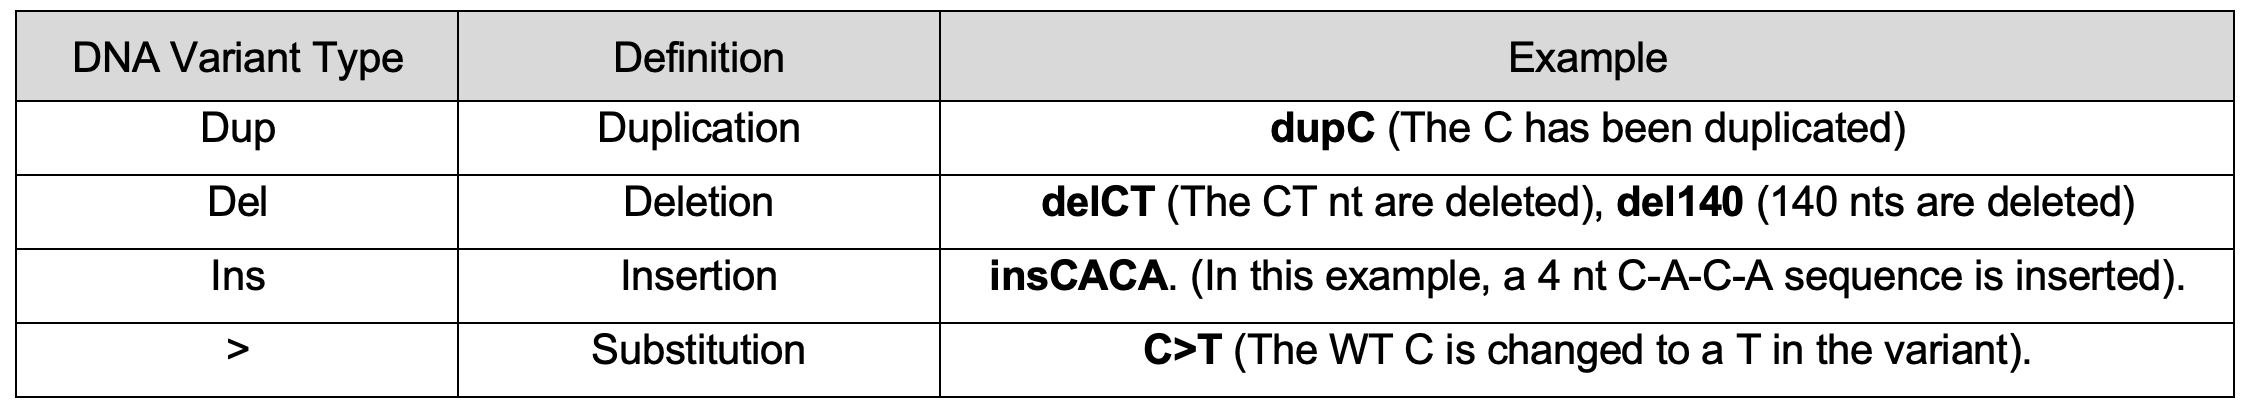
\includegraphics[width=1\linewidth]{static/images/MutationCodesTable}

}

\caption{The most common DNA varient abbreviations you are likely to see.}\label{fig:MutationCodes}
\end{figure}

The evidence track we are using to view these sequence variants is called ``Clinvar Short Variants \textless{} 50 bp''. It can be found in the ``Phenotype and Literature'' section within the list of evidence tracks below the browser window. I have it set to ``pack''. What is Clinvar? \href{https://www.ncbi.nlm.nih.gov/clinvar/}{ClinVar} is a freely accessible, public archive that reports the relationship between sequence variants in humans (DNA substitutions or indels\footnote{An small insertion or deletion mutation}) and phenotypes (benign or pathogenic). ClinVar contains submissions by clinicians \emph{and} research scientists about patients or human research subjects concerning the clinical significance of sequence variants. Some are described as pathogenic (cause disease) while others are described as benign. It's important to keep in mind that not all submissions have been verified. In other words, some data displayed in this evidence track may be inaccurate. In any case, information about short variants (\textless{} 50 bp) identified in human genes has been uploaded from the Clinvar archive into the UCSC genome browser.

Now zoom into \emph{coding} exon 1 then click on any variant. This will take you to a new page that describes the sequence variant in more detail including how the impact the sequence variant has on the nucleotide sequence (Nucleotide HGVS), the protein sequence (Protein HGVS). It may also describe any phenotype associated with the sequence variant and its clinical significance (if any).

\begin{figure}

{\centering 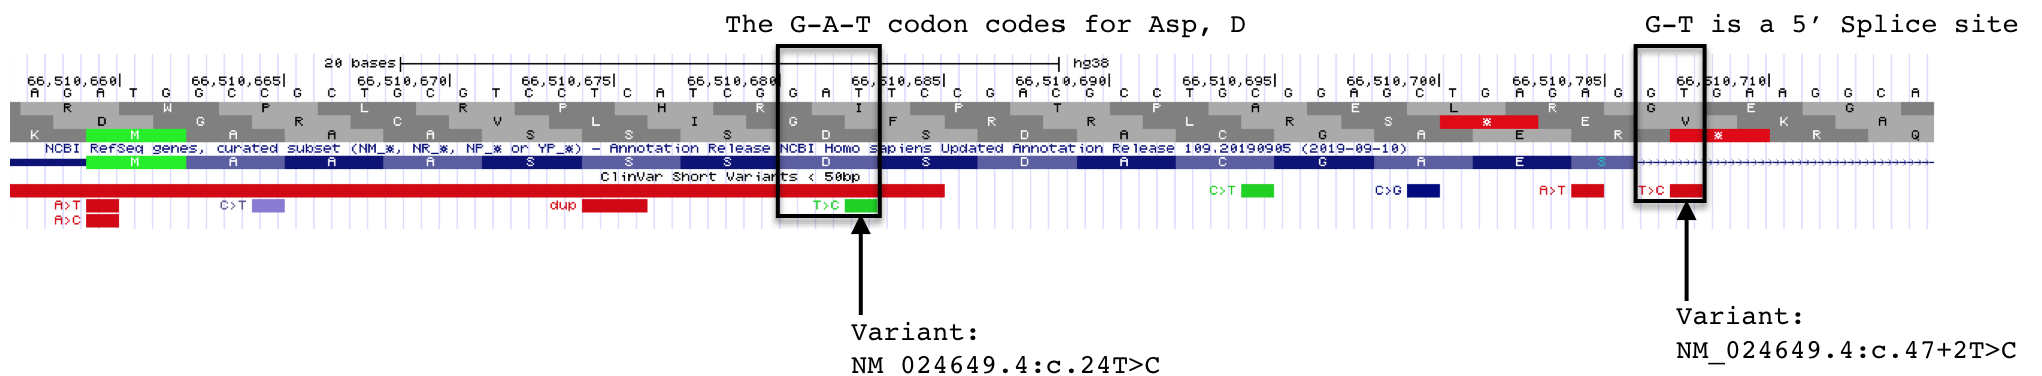
\includegraphics[width=1\linewidth]{static/images/TtoCvariant}

}

\caption{Two variants that are described in detail in the text.}\label{fig:TtoC}
\end{figure}

Now click on the the green T\textgreater C variant highlighted on the left in Figure \ref{fig:TtoC}. Notice that the ``Nucleotide HGVS'' is \textbf{NM\_024649.5:c.24T\textgreater C} (confirm for yourself so you know where you should be looking). This means that at \textbf{position 24} of the BBS1 mRNA sequence described in \href{https://www.ncbi.nlm.nih.gov/nuccore/NM_024649.5?report=GenBank}{\textbf{NM\_024649.5}}\footnote{An accession number is provided because, as you know, some genes produce multiple unique mRNAs and so the position of a given nucleotide is \emph{isoform dependent} and must be stated explicitly. In this example, you will find a T at position 24 of the sequence provided in the accession code. See for yourself! A link to the sequence was provided in the main text}, the thymine (T) is changed to cytosine (C). This is a DNA substitution. Also, the ``Protein HGVS'' is \textbf{NP\_078925.3:p.Asp8=}. This means that at \textbf{position 8} of the BBS1 protein sequence described in \href{https://www.ncbi.nlm.nih.gov/protein/NP_078925.3}{NP\_078925.3}\footnote{Again, an accession number ID is provided because some genes produce multiple unique mRNAs and thus multiple protein isoforms. So the position of a given amino acid is \emph{isoform dependent} and must be stated explicitly. In this example, you will find a D at position 8 of the sequence provided in the accession code. Again, a link to the sequence is provided in the main text}, the Asparagine (Asp, D) still codes for asparagine (=). This is a \textbf{silent} mutation (indicated with ``=''). You can confirm this by looking at the mutation in context. The \textbf{reference} codon\footnote{The reference codon is most easily defined as the ``wildtype'' version of the codon found (as is) in the genome browser. That said, it does not make sense to use the word ``wildtype'' when humans are discussed (for the same reason it does not make sense to use the word mutant). Moreover, the genome sequence uploaded to the UCSC genome browser was derived from multiple people. The word ``wildtype'' is typically only used to describe genetic model systems that are known to be inbred.} for Asparagine (Asp, D) at this position is G-A-T (Figure \ref{fig:TtoC}). In the variant, the codon changes to G-A-C (this is a T\textgreater C substitution). If you consult the genetic code (Chapter 3, Figure \ref{fig:geneticcode}) you will see that both codons code for Asparagine, Asp, D. This is also consistent with the fact that this variant is shaded green (benign). (Figure \ref{fig:HGVScodes}, includes a list of HGVS codes that describe the various impacts a mutation can have on the DNA and the protein. And click \href{http://www2.csudh.edu/nsturm/CHEMXL153/DNAMutationRepair.htm}{here} for a reminder of how to classify DNA mutations in general.

\begin{figure}

{\centering 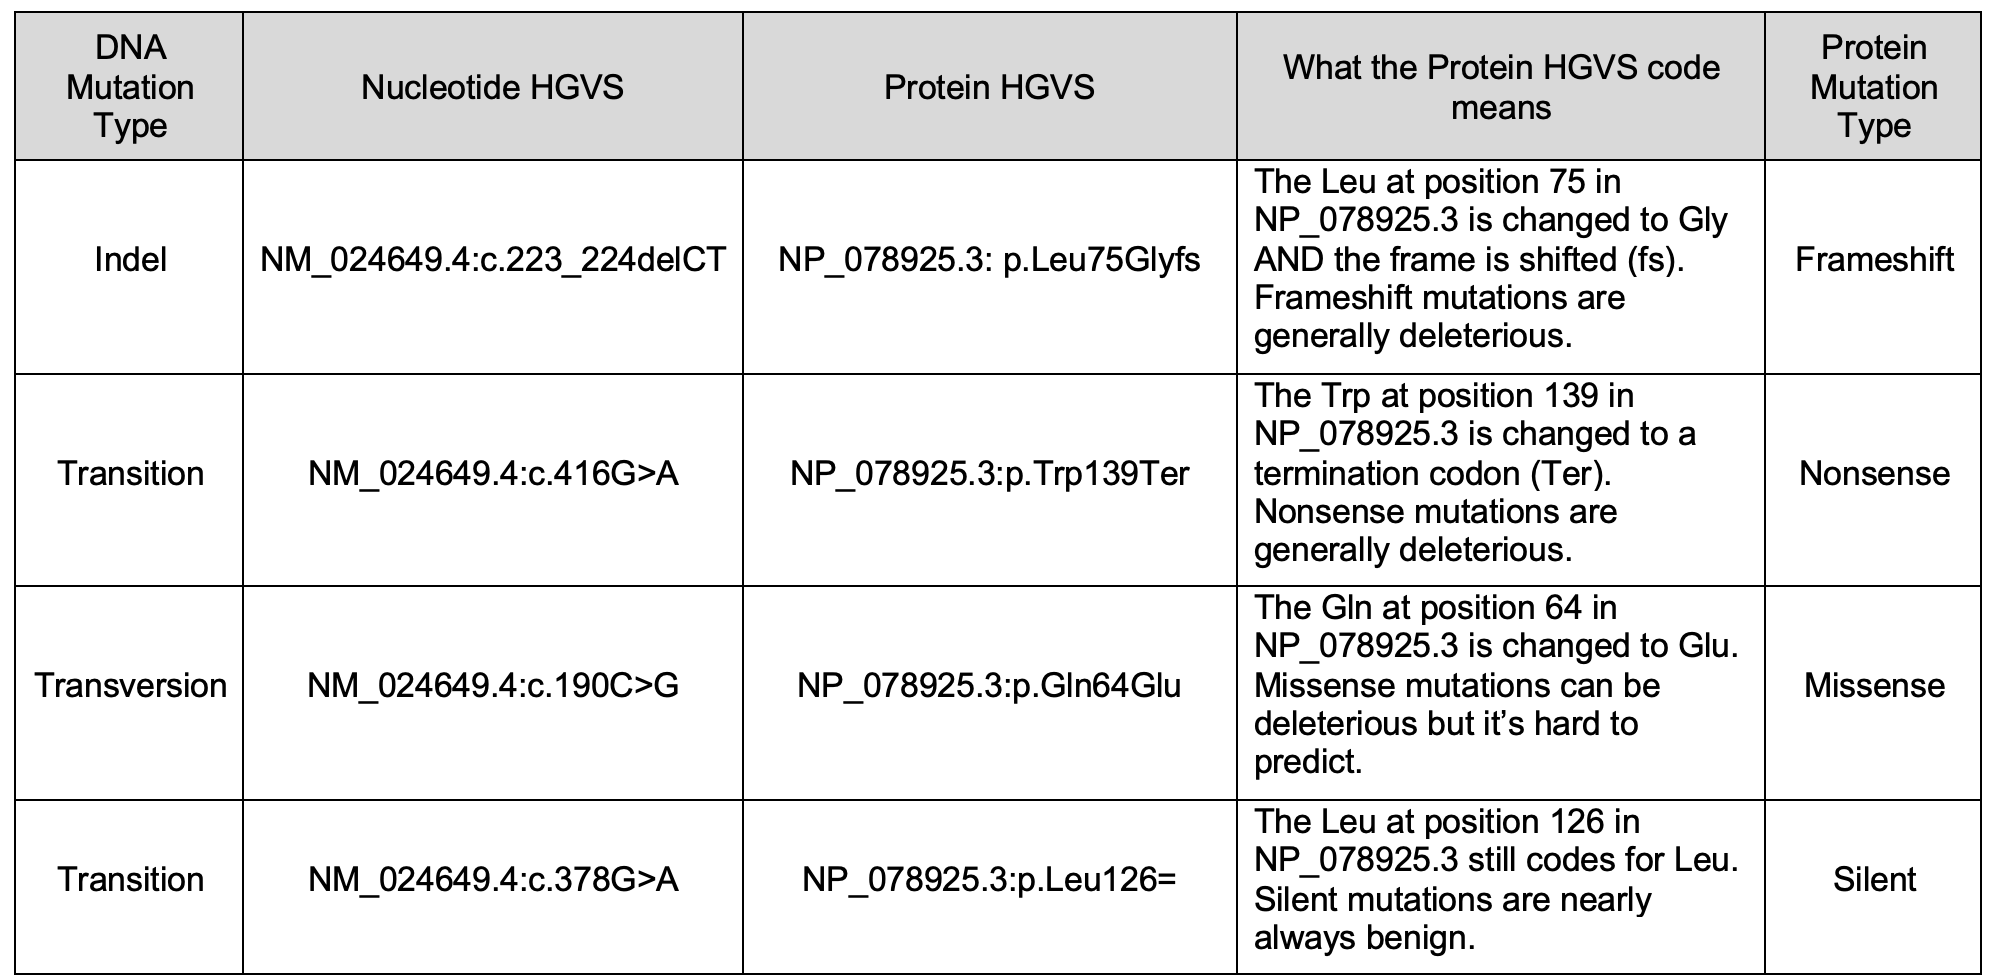
\includegraphics[width=1\linewidth]{static/images/HGVStable}

}

\caption{For examples of DNA variants and their assocated Nucleotide and Protein HGVS codes.}\label{fig:HGVScodes}
\end{figure}

Sometimes the Protein HGVS row is blank. This is often the case for splice site mutations as it is near impossible to predict what impact this type of mutation will have on the protein sequence. Will the intron remain in the mature mRNA? Will the an exon be skipped during splicing? Moreover, the position of the mutation is difficult to describe using the NM\_ code as by definition mRNAs lack introns! The following is an example of a Nucleotide HGVS description for a splice site mutation: NM\_024649.5:c.47+2T\textgreater C. In this example, position 47 is the last nucleotide of exon 1. Thus the mutation is found at 47+2 position (2nd nucleotide in the intron). In other words, the highly conserved T in the G-\textbf{T} of the 5' SS of intron 1 is mutated to a C.

Importantly, you can search for a specific variant in the UCSC genome browser using ``Nucleotide HGVS'' info (i.e.~NM\_024649.5:c.24T\textgreater C), or the ``Protein HGVS'' (i.e.~NP\_078925.3:p.Asp8=) or the ``ClinVar Variation Report'' (i.e.~NM\_024649.5(BBS1):c.24T\textgreater C (p.Asp8=)). This knowledge will come in handy when you test your understanding!

\hypertarget{test-your-understanding-23}{%
\subsection{\texorpdfstring{\href{https://docs.google.com/forms/d/e/1FAIpQLSe4661QFvixviLrC9nB5QxVFjC19_k_mI_aMwXnhcu0bFhP4Q/viewform?usp=sf_link}{Test Your Understanding}}{Test Your Understanding}}\label{test-your-understanding-23}}

To answer the following ``Test Your Understanding'' questions, use the \href{https://genome.ucsc.edu/s/megallegos/Biol\%20310\%3A\%20Module\%204\%3A\%20Mutational\%20Analysis}{``Sequence Variants''} session. You may also need to consult Figure \ref{fig:aminoacids} below to remember how amino acids are grouped according to the functional properties associated with their side chains (hydrophobic, polar uncharged etc).
Consider the coding variant \textbf{NM\_024649.5:c.235G\textgreater T} to answer the following questions:

\begin{itemize}
\tightlist
\item
  \emph{Copy and paste Nucleotide HGVS description from above into the Genome Browser window. What type of sequence variant is this (i.e.~transition, transversion or indel)?}
\item
  \emph{What is the sequence of the reference codon impacted by the G\textgreater T mutation?}
\item
  \emph{What amino acid does the reference codon code for?}
\item
  \emph{What does the reference codon become in the NM\_024649.5:c.235G\textgreater T variant?}
\item
  \emph{What amino acid does the variant codon code for (if any)?}
\item
  \emph{What type of protein variant is this?}
\end{itemize}

\begin{figure}

{\centering 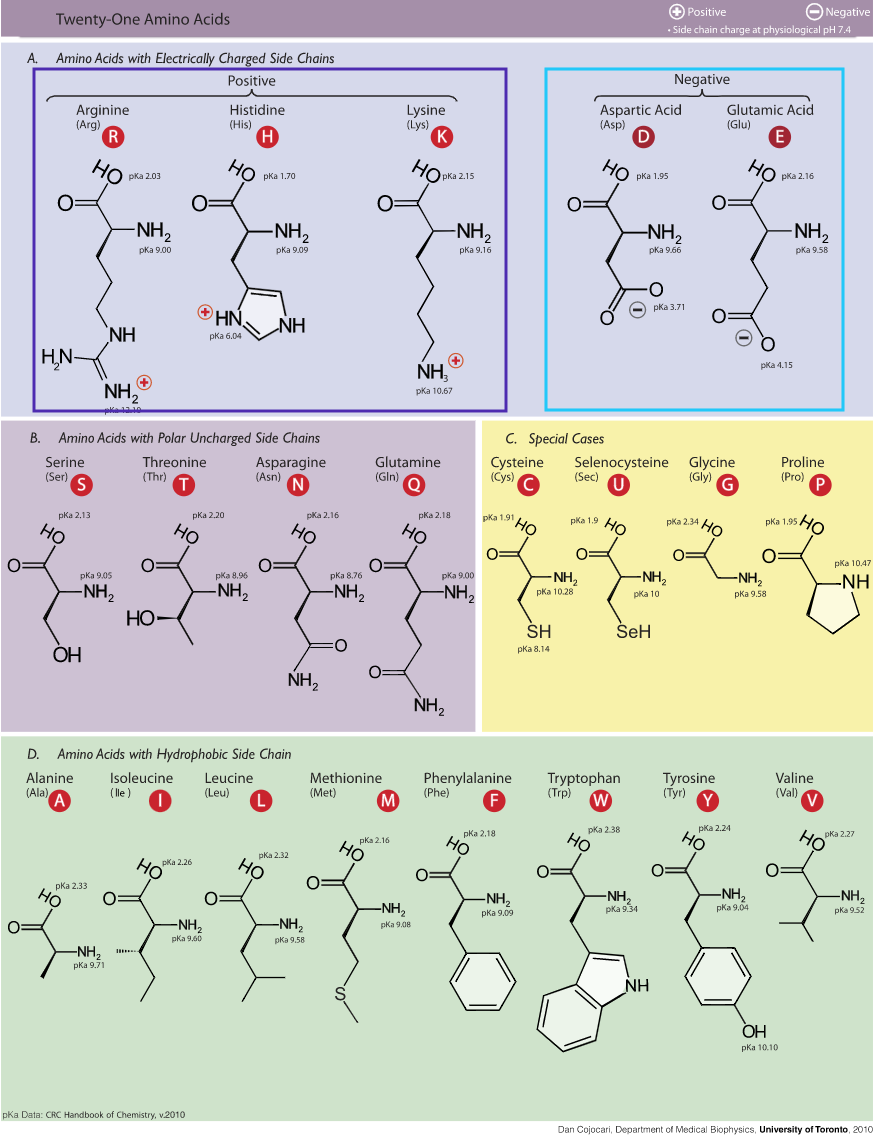
\includegraphics[width=0.75\linewidth]{static/images/aminoacidgroups}

}

\caption{Amino acid side chains can be grouped according to chemical properties. This image illustrates one way amino acids can be grouped. Image credit: [Dan Cojocari](https://commons.wikimedia.org/w/index.php?curid=9179304).}\label{fig:aminoacids}
\end{figure}

\hypertarget{test-your-understanding-24}{%
\subsection{\texorpdfstring{\href{https://docs.google.com/forms/d/e/1FAIpQLSeFPVWrhrsiNtMIHhQF2eNraOkg3sjLqcY-q8y9FtL7H_N5eA/viewform?usp=sf_link}{Test Your Understanding}}{Test Your Understanding}}\label{test-your-understanding-24}}

To answer the following ``Test Your Understanding'' questions, use the \href{https://genome.ucsc.edu/s/megallegos/Biol\%20310\%3A\%20Module\%204\%3A\%20Mutational\%20Analysis}{``Sequence Variants''} session.
Now consider the coding variant \textbf{NM\_024649.5:c.41C\textgreater G} to answer the following questions:

\begin{itemize}
\tightlist
\item
  \emph{Copy and paste Nucleotide HGVS description from above into the Genome Browser window. What type of sequence variant is this (i.e.~transition, transversion or indel)?}
\item
  \emph{What is the sequence of the reference codon impacted by the C\textgreater T mutation?}
\item
  \emph{What amino acid does the reference codon code for?}
\item
  \emph{What does the reference codon become with the NM\_024649.5:c.41C\textgreater G variant?}
\item
  \emph{What amino acid does the variant codon code for (if any)?}
\item
  \emph{What type of protein variant is this?}
\end{itemize}

Now consider the coding variant \textbf{NM\_024649.5:c.240C\textgreater T} to answer the following questions:

\begin{itemize}
\tightlist
\item
  \emph{Copy and paste Nucleotide HGVS description from above into the Genome Browser window. What type of sequence variant is this (i.e.~transition, transversion or indel)?}
\item
  \emph{What is the sequence of the reference codon impacted by the C\textgreater T mutation?}
\item
  \emph{What amino acid does the reference codon code for?}
\item
  \emph{What does the reference codon become with the NM\_024649.5:c.240C\textgreater T variant?}
\item
  \emph{What amino acid does the variant codon code for (if any)?}
\item
  \emph{What type of protein variant is this?}
\end{itemize}

General Questions about mutations.

\begin{itemize}
\tightlist
\item
  \emph{What type of sequence variants lead to a frameshift mutation (transition, transversion, indel)?}
\item
  \emph{By definition, where must frameshift mutations be located (i.e.~exons, introns, 5' UTR, 3' UTR, promoter)?}
\item
  \emph{By definition, where must splice site mutations be located (i.e.~exons, introns, 5' UTR, 3' UTR, promoter)?}
\item
  \emph{By definition, where must nonsense mutations be located (i.e.~exons, introns, 5' UTR, 3' UTR, promoter)?}
\end{itemize}

Step back and look at a larger region surrounding BBS1. Specifically, click on the link for \href{https://genome.ucsc.edu/s/megallegos/Biol\%20310\%3A\%20Module\%204\%3A\%20Mutational\%20Analysis}{``Sequence Variants''} session then zoom out 10X. This region now includes neighboring genes including MRPL11, DPP3, BBS1, ZDHHC24, ACTN3 and CTSF.

\begin{itemize}
\tightlist
\item
  \emph{Copy and paste a nucleotide HGVS code for any frameshift mutation that maps to BBS1}
\item
  \emph{Pathogenic sequence variants map to two genes in this region. Choose the two among MRPL11, DPP3, BBS1, ZDHHC24, ACTN3 and CTSF?}
\end{itemize}

\hypertarget{for-discussion-4}{%
\section{\texorpdfstring{\href{https://docs.google.com/forms/d/e/1FAIpQLSda-6Xh3SbF8zzKhoQVZ6biWLkzigculLabj8y3Jg1I4Yc5KA/viewform?usp=sf_link}{For Discussion}}{For Discussion}}\label{for-discussion-4}}

\begin{enumerate}
\def\labelenumi{\arabic{enumi}.}
\tightlist
\item
  Some genes don't have any variants associated with them. Why do you think this is? More than one answer is possible.
\item
  Find the sequence variant that maps to the gene, CCS (Nucleotide HGVS: NM\_005125.2:c.487C\textgreater T). It suggests that it might lead to neurodegeneration but it is rated as ``uncertain significance''. How likely do you think it is that this is a pathogenic allele. Use any tool (including Google searches, your knowledge of genetics and reasoning abilities) to argue one way or the other (there are no right answers).
\end{enumerate}

\hypertarget{homework-1}{%
\section{\texorpdfstring{\href{https://drive.google.com/file/d/11T71xL2ylto_hP32Uo560bUnb0kbLp61/view?usp=sharing}{Homework}}{Homework}}\label{homework-1}}

© 2019, Maria Gallegos. All rights reserved.

\hypertarget{orthology-and-disease-models}{%
\chapter{\texorpdfstring{\emph{Orthology and Disease Models}}{Orthology and Disease Models}}\label{orthology-and-disease-models}}

Genetic model organisms like yeast, worms, flies, fish and mice play a critical role in the advancement of biomedical research (Figure \ref{fig:modelorganisms}). Each offers unique advantages and all allow the opportunity to investigate gene function and model human disease in an organism that is amenable to genetic, molecular and biochemical studies. Moreover, research in model organisms is cheaper, faster and more ethical than research on humans! A list of advantages and disadvantages for each of the most common species studied today are shown in Figure \ref{fig:modelsystems}.

\begin{figure}

{\centering 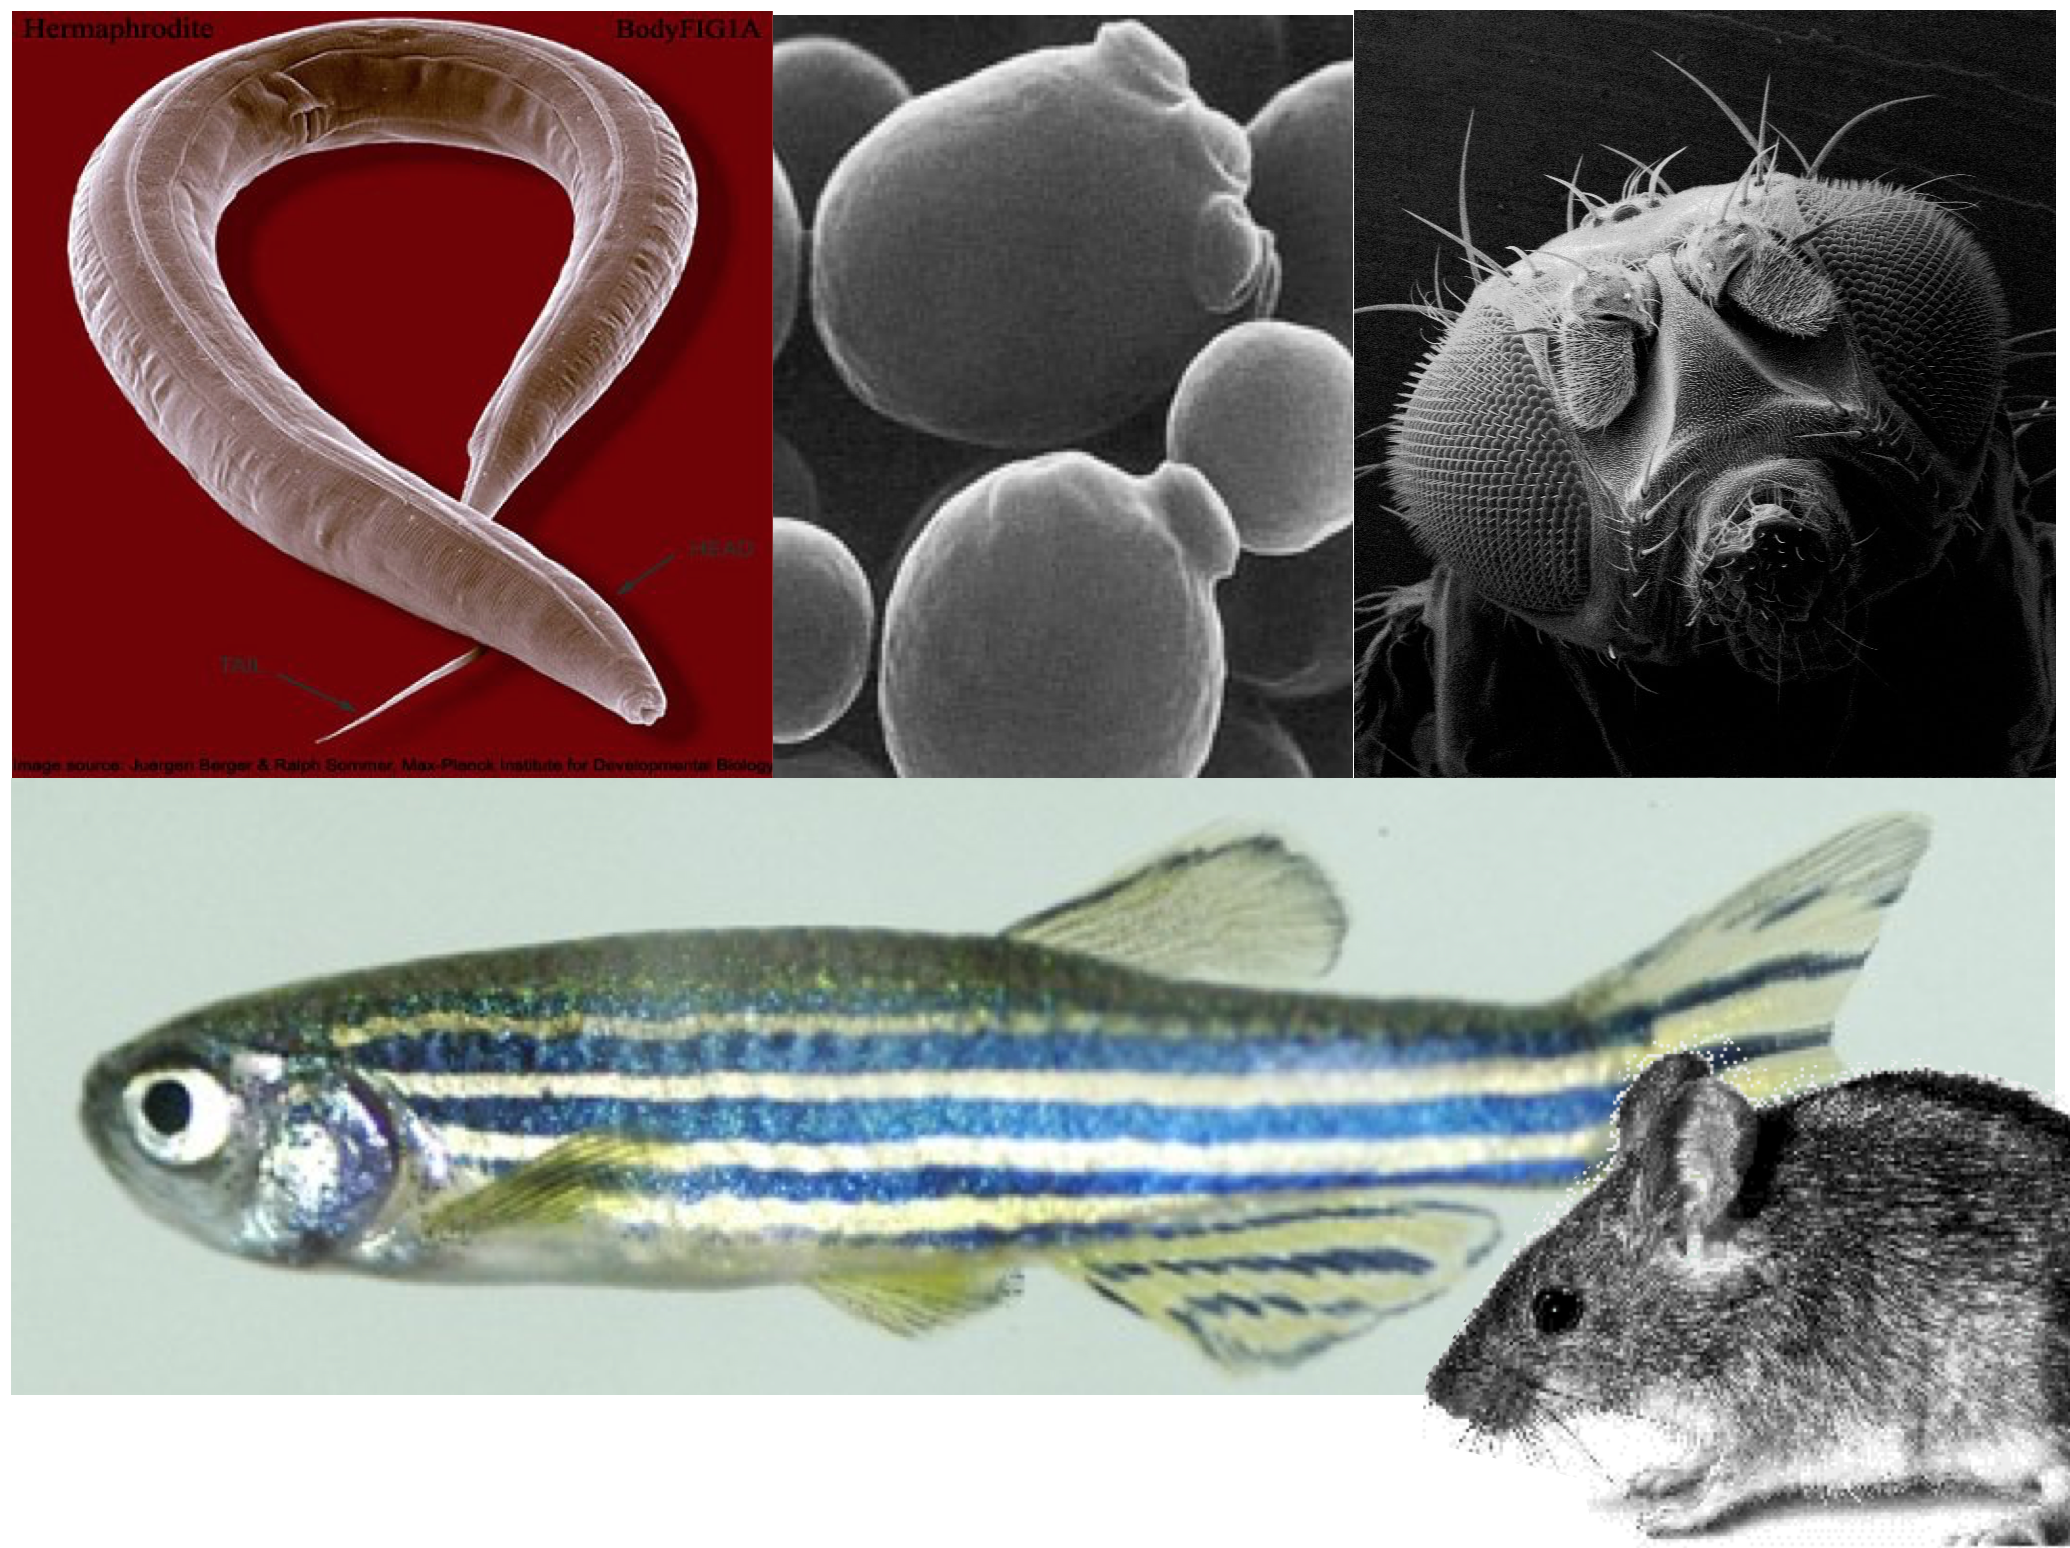
\includegraphics[width=0.6\linewidth]{static/images/modelsystems}

}

\caption{Popular model organisms used in genetic research. Clockwise from top left: *Caenorhaditis elegans* (round worm), *Saccharomyces cerevisiae* (budding yeast), *Drosophila melanogaster* (fruit fly), *Mus musculus*, (house mouse) and *Danio rerio* (zebrafish). Image sources: worm image from [Wormatlas](https://www.wormatlas.org/hermaphrodite/introduction/Introframeset.html), yeast image by Alan Wheals, University of Bath, UK., fly, mouse and fish image sources unknown.}\label{fig:modelorganisms}
\end{figure}

\begin{figure}

{\centering 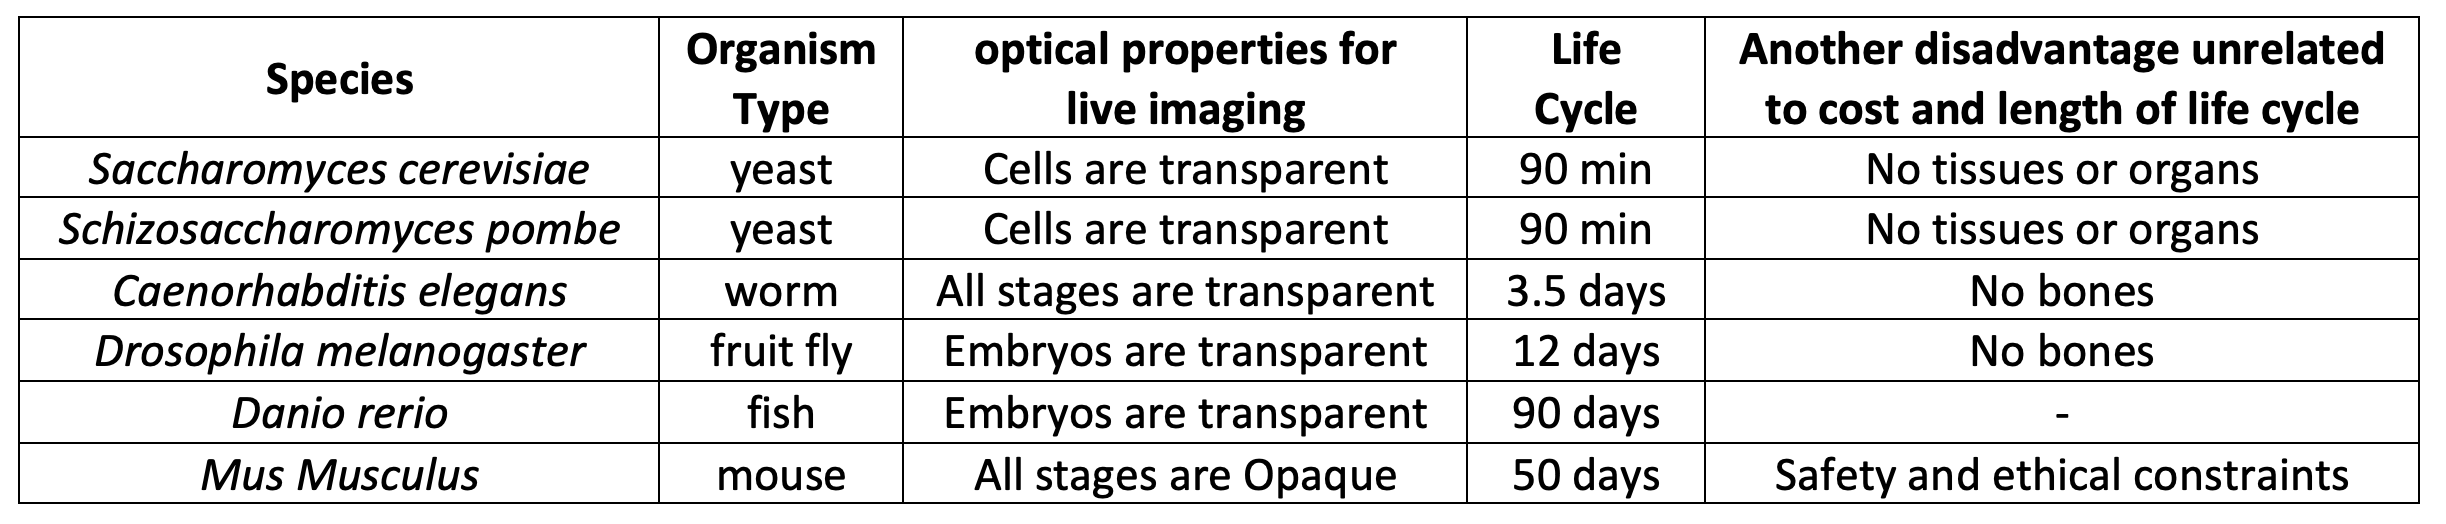
\includegraphics[width=1\linewidth]{static/images/modelorganisms}

}

\caption{Advantages and disadvantages of the common model organisms used in genetic research listed from cheapest (yeast) to most expensive (mice).}\label{fig:modelsystems}
\end{figure}

While at the surface humans appear to have little in common with mice, fish, flies, worms or fungi, this approach works. Why? \href{https://en.wikipedia.org/wiki/Cell_theory\#:~:text=All\%20known\%20living\%20things\%20are,total\%20activity\%20of\%20independent\%20cells.}{Cell Theory} states that ``all cells come from pre-existing cells''. And in fact, a significant percentage of genes from these ancestral cells persist in some form in Eukaryotes today. Despite nearly 1 billion years of evolution, many gene products are recognizable at the amino acid sequence level and in some cases are functionally interchangeable!

For example, a human gene called BCL2 was found that inhibits \textbf{programmed cell death} in human cells grown in a dish (Vaux et al.~1988). Programmed cell death is a biological process that has been observed in all animals studied to date. When certain cells are no longer needed, they ``commit suicide'' by activating an intracellular death program. But programmed cell death must be kept under control. Too much death is also problematic. In 1992, Vaux et al.~discovered that if you inject human \emph{BCL2} fused downstream to a worm heat-shock promoter\footnote{A promoter that is activated by heat. With heat shock, the promoter will initiate high levels of transcription!} its progeny\footnote{offspring or descendants of an animal, or plant - online dictionary} not only expressed the human gene when heat shocked but also had \textbf{\emph{less}} programmed cell death! See Figure \ref{fig:BCL2rescue} A and B.

\begin{figure}

{\centering 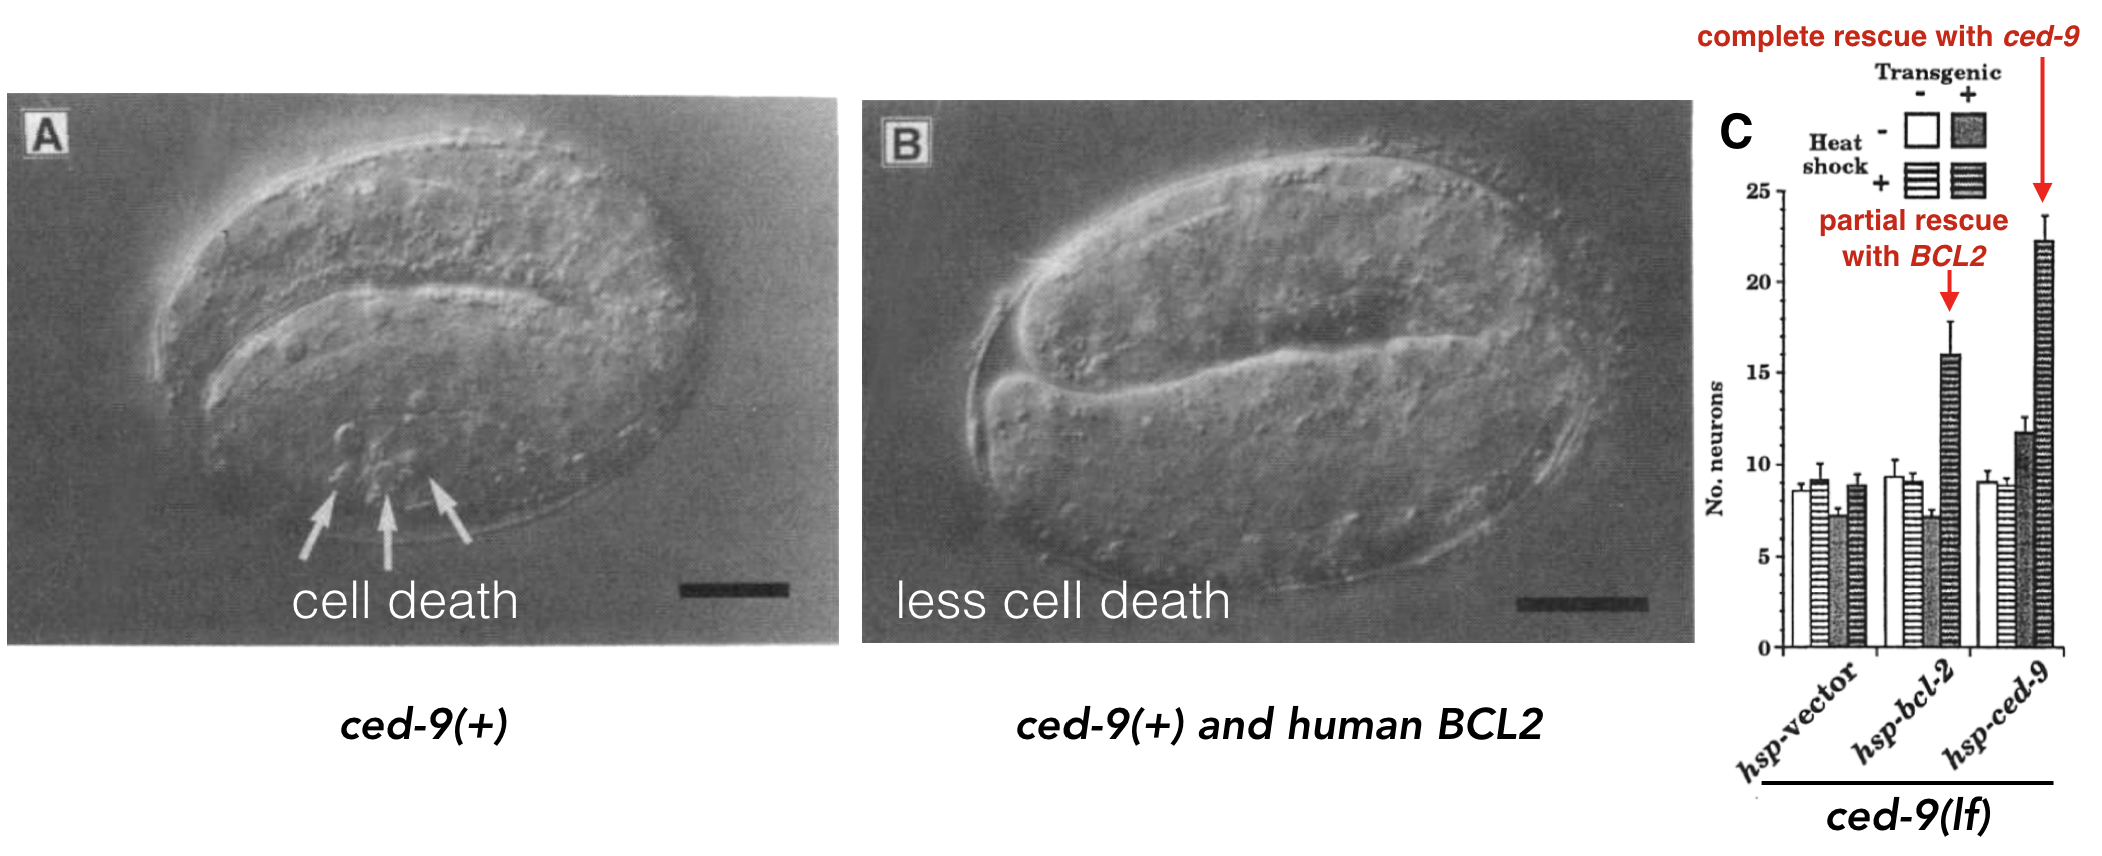
\includegraphics[width=1\linewidth]{static/images/BCL2}

}

\caption{A) Normal worm development includes a certain amount of programmed cell death. B) When human *BCL2* is expressed in worm embryos, less cell death is observed (Vaux et al. 1992). *+* indicates, wildtype allele. C) Data demonstrating that human *BCL2* is able to partially rescue the *ced-9* loss-of-function mutant phenotype (Hengartner and Horvitz, 1994). }\label{fig:BCL2rescue}
\end{figure}

A worm gene called \emph{ced-9} was later found to function similarly. In loss of function \emph{ced-9} mutants, more cells died suggesting that wildtype \emph{ced-9} (like \emph{BCL2}) inhibits programmed cell death. In subsequent experiments, Hengartner and Horvitz partially \textbf{rescued} \emph{ced-9} loss of function mutants with the human \emph{BCL2} gene! In other words, \emph{ced-9} mutant worms expressing human \emph{BCL2} looked more like wild type (Figure \ref{fig:BCL2rescue} C). Dr.~Vaux, the first author explained in an \href{https://www.nature.com/articles/4401439}{interview}: ``This meant that the human BCL2 protein must be interacting with the worm's cell death mechanism. The fact that human \emph{BCL2} could work in a worm suggested that human \emph{BCL2} can interact with whatever proteins the worm CED-9 protein interacts with. That, in turn, suggests that not only the gene but also the pathway of cell death is likely to be universal.'' That is one billion years of evolution separating worms and humans! This is strong evidence that human \emph{BCL2} and worm \emph{bcl-2} are \textbf{orthologs} a term that describes two genes in distinct species that evolved from an ancestral gene present in the last common ancestor.

In 2014, Dr.~Ethan Perlstein created Perlara, a biotech Public Benefit Corporation which aimed to accelerate the discovery of treatments for rare genetic diseases through the use of simple model organisms. While this company has since shut down\footnote{an early backer and partner withdrew from a licensing deal which triggered a fatal downward spiral} they were ultimately successful in in their efforts.

In one example, Perlara created yeast, worm and fly models of a rare congenital disorder of glycosylation called PMM2-CDG\footnote{According to Wikipedia, \textbf{glycosylation} is a process whereby a carbohydrate is attached to a hydroxyl or other functional group of another molecule (often a lipid or protein)} caused by mutations in the PMM2 gene\footnote{According to Genetics Home Reference, the PMM2 gene produces an enzyme called phosphomannomutase 2. This enzyme is involved in glycosylation (see earlier footnote), which acts by attaching groups of sugar molecules to proteins}. From their initial studies they knew they needed a drug that would boost the enzymatic activity of PMM2. To identify such a drug, Perlara performed a drug repurposing screen\footnote{searching through a library of drugs already available and approved for a different disorders} using the worm model Perlara created for PMM2-CDG. Eperlstat, a drug normally used to treat diabetic neuropathy looked promising and was later shown to boost PMM2 enzyme function in PMM2-CDG patient fibroblasts\footnote{PMM2-CDG patient fibroblasts are skin cells taken from patients with the PMM2 disorder.}! Finally in early 2020 Dr.~Ethan Persltein began treatment of the first human patient, Maggie Carmichael. After 6 months, the change has been dramatic (Figure \ref{fig:PMM2Perlquest}).

\begin{figure}

{\centering 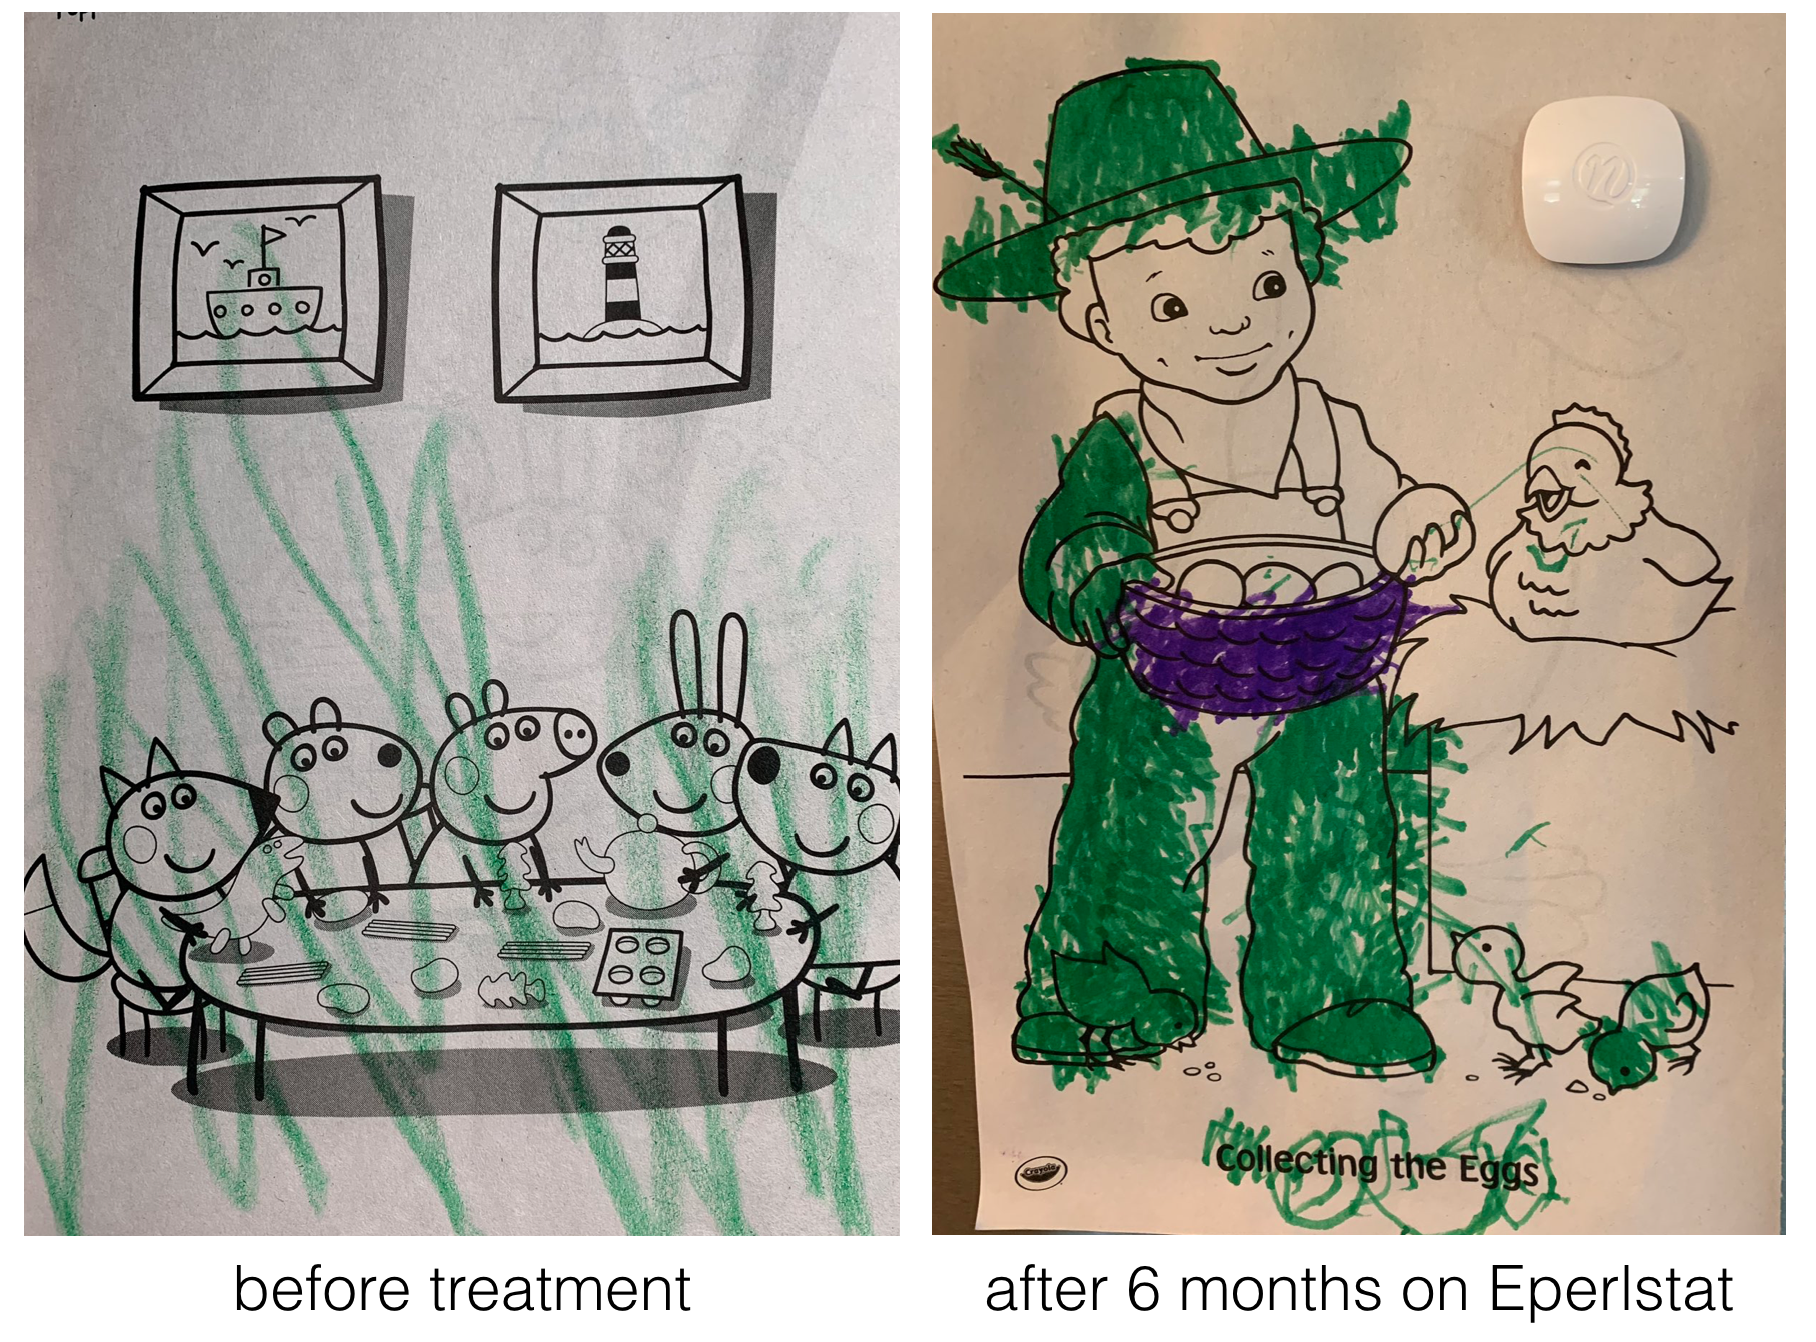
\includegraphics[width=0.5\linewidth]{static/images/MaggiesPerlquest}

}

\caption{Image courtesy of Holly and Dan Carmichael}\label{fig:PMM2Perlquest}
\end{figure}

Luckily for us, they also left behind a rich collection of blogs and publications that outline their approach for the benefit of others. The ones about the animal models for PMM2-CDG are listed below:

\begin{enumerate}
\def\labelenumi{\arabic{enumi}.}
\tightlist
\item
  \href{https://www.g3journal.org/content/ggg/9/2/413.full.pdf}{Yeast Models of Phosphomannomutase2 Deficiency, a Congenital Disorder of Glycosylation}
\item
  \href{https://www.perlara.com/blog/developing-pmm2-drosophila-models/}{Modeling PMM2 deficiency in Drosophila}.
\item
  \href{https://www.perlara.com/blog/a-chemical-modifier-screen-for-pmm2-deficiency-in-worms/}{A chemical modifier screen for PMM-2 deficiency in worms}.
\end{enumerate}

\textbf{The bottom line: The accurate identification of an orthologous pair between a model organism and humans is a prerequisite for creating a human disease model}. A simple and widely used approach to identify putative orthologs is known as the reciprocal best hit (RBH) method\footnote{Sometimes called the bidirectional best hit (BBH) method}. In fact, a recent study concludes that a high proportion of RBH pairs are likely to be true orthologs (Dalquen and Dessimoz, 2013).

\hypertarget{performing-a-reciprocal-best-hit-analysis}{%
\section{Performing a Reciprocal Best Hit Analysis}\label{performing-a-reciprocal-best-hit-analysis}}

To find a putative ortholog of a human gene, you start with a human protein (a gene product) as a \textbf{query}\footnote{defined by the online dictionary as ``a question, especially one addressed to an official or organization''. In our context, your human protein sequence \emph{implies} the question: Are there proteins in my model system of choice that are similar to this human protein sequence?} to search a protein database from a model organism of your choice. This is called performing a \textbf{BLASTP}\footnote{BLAST finds regions of similarity between biological sequences. The program compares nucleotide or protein sequences to sequence databases and calculates the statistical significance. The ``p'' in BLASTP searches protein databases with protein queries. BLASTN is for searching nucleotide databases with nucleotide sequences}. Your goal is to identify one protein in your model organism of choice with the \textbf{best} sequence similarity to the human protein you used as your query. This is your \textbf{best hit} also known as your \textbf{top hit}. You then use this ``best hit'' from the model organism as a query to search the human protein database (\textbf{a reciprocal BLASTP}). If your ``best hit'' in the human database is a gene product of the gene you used as a query in your first BLAST then you have found a \textbf{``Reciprocal Best Hit''} (Figure \ref{fig:RBH}). In other words, a reciprocal best hit succeeds at identifying a pair of orthologs when it identifies a pair of \emph{genes} that are \emph{eachother's} best hit. If successful, you now have evidence that a specific gene pair are putative orthologs.

\begin{figure}

{\centering 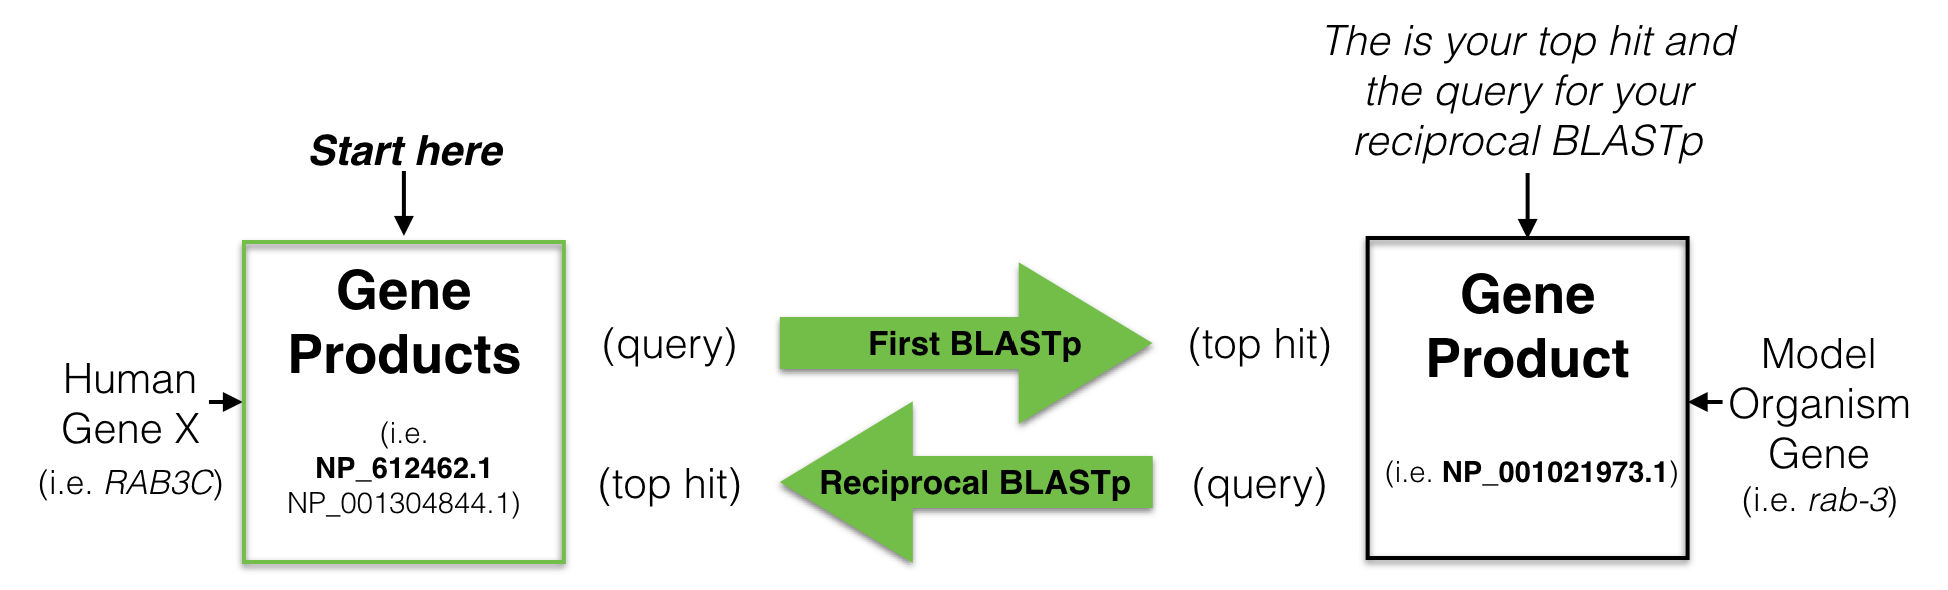
\includegraphics[width=1\linewidth]{static/images/RBHanalysis}

}

\caption{A schematic diagram to explain a reciptrocal best hit analysis. See text for details.}\label{fig:RBH}
\end{figure}

\hypertarget{rbh-analyis-of-human-bbs1-first-blastp.}{%
\section{RBH analyis of human BBS1: First BLASTP.}\label{rbh-analyis-of-human-bbs1-first-blastp.}}

To start, click the link for \href{https://genome.ucsc.edu/s/megallegos/Biol\%20310\%20Module\%201}{Module One}. Click on the BBS1 schematic within the NCBI Refseq Gene Predictions Track to open the gene information page. In the gene information page, click on the Protein Accession link (Format: NP\_XXXXX.X) to open the protein information page. At the top right corner of the protein information page, under the section entitled, ``Analyze this sequence'', click on ``Run BLAST''. A BLASTP page will open. On the BLASTP page, notice that the protein accession code for BBS1 has been entered into the query sequence window. This is the ``Query ID'' for your first BLASTP search. Keep all default settings \emph{except} the following: Choose the ``Reference Proteins (Refseq proteins)'' from the pull down menu for your \textbf{Database}. Then type \emph{``Caenorhabditis elegans''} into the query window for ``Organism''. As you type, a drop down menu will appear for your convenience. Choose the correct species on this list. \emph{Caenorhabditis} is not easy to spell. Best to just type \emph{``elegans''}! Finally, scroll to the bottom of the BLASTP page, click ``BLAST'' and wait (Figure \ref{fig:FIRSTBLAST}).

\begin{figure}

{\centering 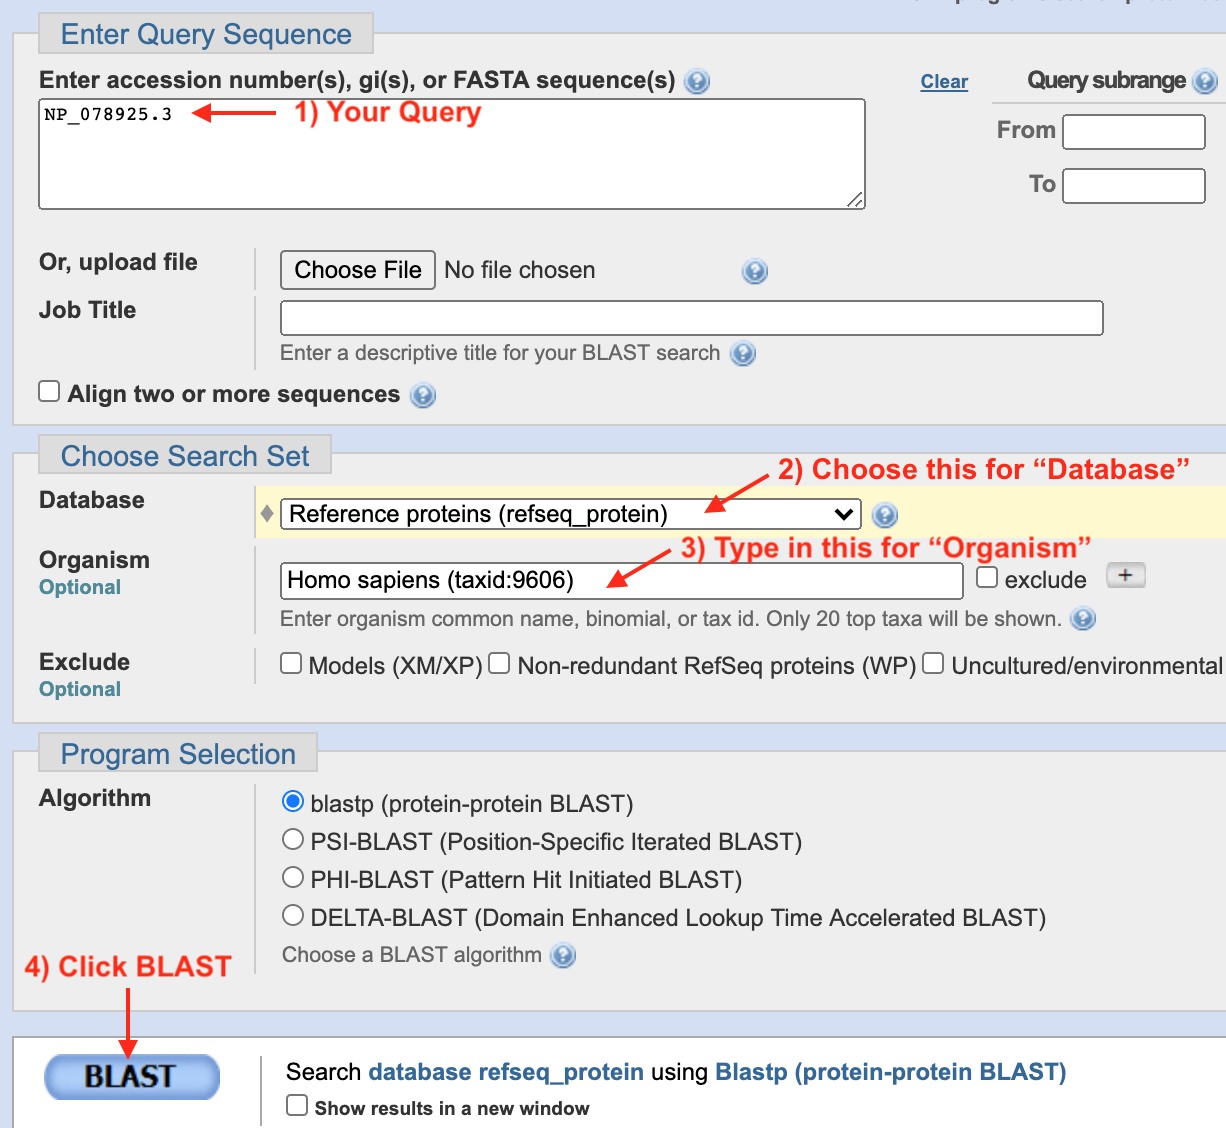
\includegraphics[width=0.75\linewidth]{static/images/firstBLASTP}

}

\caption{1) If you get to this page via the protein information page, your Refseq Accession number will already be present in the query window. If you get here via Google, you can type in your Refseq Accession number manually. To simplify your results, 2) choose **Reference Proteins (Refseq Proteins)** for your **Database**. 3) Type in your model system of choice in the **Organism** window. In most cases, you need to know the latin species name. 4) Now click **BLAST** then wait.}\label{fig:FIRSTBLAST}
\end{figure}

Your results page will appear after some time. It will contain multiple tabs near the top of the page including ``Descriptions'', ``Graphic Summary'', ``Alignments'' and ``Taxonomy''. You are welcome to ``click around'' and play but for now we will stick with the ``Descriptions'' tab. This tab includes a table that lists all your ``hits'' that have significant similarity to your query sequence. The table includes seven columns. In the descriptions column you will find the common or systematic name of the protein and the species in brackets. Columns 2, 3 and 5 quantify how similar your query is to the protein listed. Columns 2 and 3 should be high numbers while column 5 should be tiny. More intuitive measures of sequence similarity include ``Query Cover'' and ``Percent Identity''. ``Query Cover'' describes what fraction of the ``hit'' aligns with your query. ``Percent Identity'' describes the fraction of the \textbf{alignment} that are identical between the two sequences. The last column provides the accession number of the ``hit''. The ``best hit'' or ``top hit'' is the hit in the top row (row 1). It should have (in sum) the largest ``Max Score'', ``Total Score'', ``Query Coverage'' and ``Percent Identity''. It should also have the lowest ``E value''. To see the pairwise alignment of your top hit and query, click the ``Alignment'' tab. Scroll down to see the complete alignment. Each alignment includes a description of the hit including the protein name (descriptive or systematic) and the species in brackets. The next line includes the ``Sequence ID'' (Refseq Accesion Code) and the ``Length'' of the hit (in our example, this is the number of amino acids).

\hypertarget{understanding-a-pairwise-alignment}{%
\section{Understanding a Pairwise Alignment}\label{understanding-a-pairwise-alignment}}

Now that you have done your first BLASTP, you need to understand how to ``read'' a pairwise alignment. Figure \ref{fig:pairwise} includes a small portion of a pairwise alignment in two different formats. The default format is displayed in A. The first row of the alignment (A and B) contains the query sequence (from amino acids 196 to 255). This sequence is aligned to and stacked on top of a protein sequence that has significant sequence simalarity with the query (from amino acids 183 to 240). This aminco acid sequence is displayed in the ``Sbjct'' row. The middle row of the alignment in Figure \ref{fig:pairwise}A displays the \emph{degree} of matching between the two sequences at each position. ``+'' is placed in each column of the alignment where the amino acids in the ``query'' and ``sbjct'' are similar but not identical (conserved). An amino acid (in single letter code) is placed in the column where the amino acids in the ``query'' and ``sbjct'' are identical. Columns where the the amino acids in the ``query'' and ``sbjct'' are unrelated are left blank. The format in Figure \ref{fig:pairwise}B emphasizes the differences in the alignment as a ``.'' is placed in columns where in the ``query'' and ``sbjct'' are identical. In both formats, a \textbf{gap} in the alignment is represented by ``-``. Each gap suggests that during the process of evolution, one or more complete codons were either deleted in the query gene or added in the subject gene. It is not clear from a simple pairwise alignment if the ancestral gene looked more like the subject or query gene.

\begin{figure}

{\centering 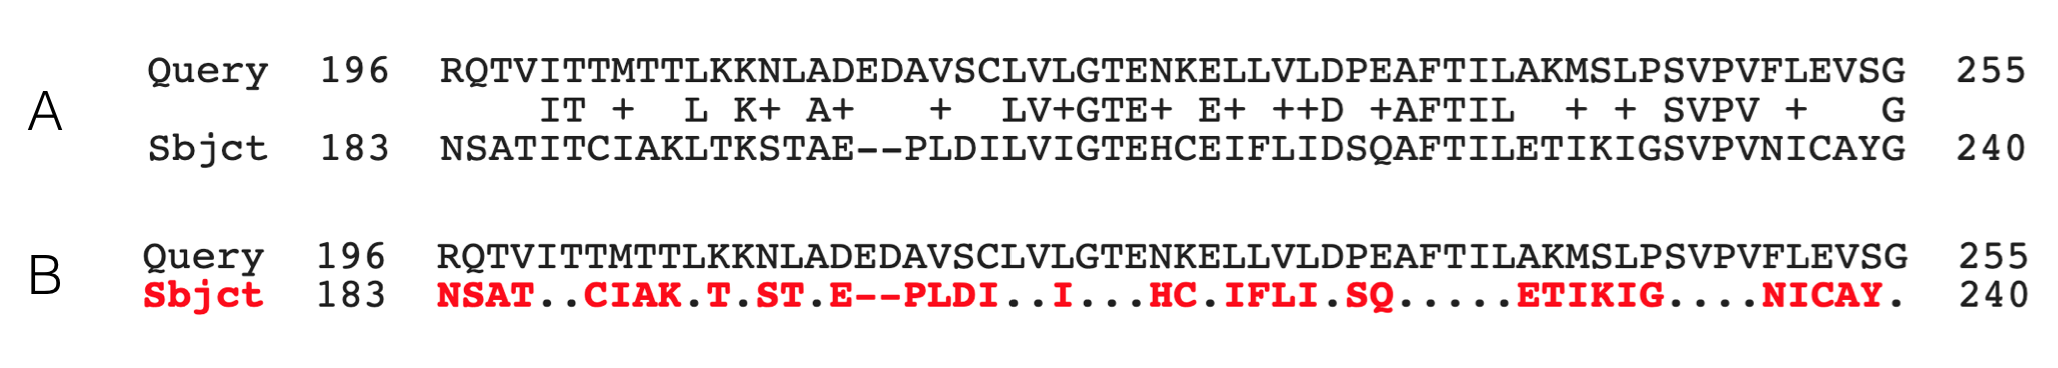
\includegraphics[width=1\linewidth]{static/images/TwoPairwiseAlignments}

}

\caption{A single row (small portion) of a pairwise alignment displayed in two different formats. The default format is shown on top. See text for details.}\label{fig:pairwise}
\end{figure}

To better understand how the numbering system works in a pairwise alignment, see if you can confirm the following statements. In Figure \ref{fig:pairwise}, there is a ``Q'' at position 197 of the Query sequence. Q197 aligns with an S at position 184 of the Sbjct. The ``I'' at position 200 of the Query is identical to the ``I'' at position 187 of the Sbjct. The ``M'' at position 203 of the Query is not identical but conserved with the ``I'' at position 190 in the Sbjct (methionine (M) and isoleucine (I) are both hydrophobic). Finally, there is a ``P'' at position 200 of the Sbjct. Can't confirm? Note that \textbf{gaps in an alignment are NOT counted.}

\hypertarget{test-your-understanding-25}{%
\subsection{\texorpdfstring{\href{https://docs.google.com/forms/d/e/1FAIpQLSeACOPQeUC_YCjHqISD95DYyEpiSjJPHThNVxIYZ0v1Okmd2g/viewform?usp=sf_link}{Test Your Understanding}}{Test Your Understanding}}\label{test-your-understanding-25}}

Use the pairwise alignment from your top hit of your first BLASTP (human BBS1 as your Query, C. elegans as your Subject, the ``Reference proteins'' as your database) to answer the following questions:

\begin{itemize}
\tightlist
\item
  \emph{There is a gap in the second alignment row with the sequence, \textbf{LSS -- -- IPS}, in the Subject row (the worm sequence). The S next to the gap in this sequence is at position 87. At what position is the P?}
\item
  \emph{What is the amino acid at position 260 of the human BBS1 protein (Use single letter amino acid code)?}
\item
  \emph{Consider the worm amino acid that is aligned with the human amino acid at position 260. What is it? (Use single letter amino acid code)?}
\item
  \emph{Consider the worm amino acid that is aligned with the human amino acid at position 260. Where is it? What position is it at within the worm protein? (Insert whole number)?}
\item
  \emph{Is amino acid 260 in humans identical, similar or unrelated to the worm amino acid it is aligned to?}
\item
  \emph{What is the amino acid at position 479 of the worm BBS1 protein? (use the single letter amino acid code)?}
\item
  \emph{Is amino acid at position 479 in worms identical, similar or unrelated to the human amino acid it is aligned to?}
\item
  \emph{What is the Refseq accession Code for the top hit (Hint: It should be begin with NP\_ or XP\_ and be from the C. elegans protein database?}
\item
  \emph{What is the \% identity of your top hit in C. elegans?}
\item
  \emph{What is the \% query cover of your top hit in C. elegans?}
\end{itemize}

\hypertarget{rbh-analyis-of-human-bbs1-reciprocal-blastp.}{%
\section{RBH analyis of human BBS1: Reciprocal BLASTP.}\label{rbh-analyis-of-human-bbs1-reciprocal-blastp.}}

Now that you have performed your first BLASTP, you are ready to look to see if the best hit in worms is a ``reciprocal best hit''. First step, identify your top hit from first BLASTP. You can either go to the ``Descriptions'' tab and click on the link to the Refseq Accession Code (Format: NP\_XXXXX.X) in the ``Accession'' Column for your \textbf{top hit}. Or you can go to the ``Alignment'' tab and click on the Refseq Accession Code link listed for ``Sequence ID:''. Either will take you to the same protein information page for your top hit in \emph{C. elegans}. Again, at the top right of the protein information page, under the section entitled, ``Analyze this sequence'', click on the word ``Run BLAST''. The BLASTP page will open. Again, on the BLASTP page, the accession code will have been entered into the query sequence window for you. This is your new ``Query ID'' for your reciprocal BLASTP. Keep all default settings \emph{except} the following: Choose the ``Reference Proteins (Refseq proteins)'' from the pull down menu for your \textbf{Database}. Then type \emph{``Homo sapiens''} into the query window for ``Organism''. As you type, a drop down menu will appear for your convenience. Choose the correct species on this list. Finally, scroll to the bottom of the BLASTP page, click ``BLAST'' and wait.

\hypertarget{test-your-understanding-26}{%
\subsection{\texorpdfstring{\href{https://docs.google.com/forms/d/e/1FAIpQLSctC_EHT6uey1_zYviwwxNJRCgWAM-bKxlkiJawl5HfZk6siw/viewform?usp=sf_link}{Test Your Understanding}}{Test Your Understanding}}\label{test-your-understanding-26}}

Perform your Reciprocal BLASTp to answer the following questions:

\begin{itemize}
\tightlist
\item
  \emph{For your reciprocal BLAST hit analysis, what is the Refseq protein accession code for your query?}
\item
  \emph{What is the Refseq protein accession code for the top hit in homo sapiens?}
\item
  \emph{Is this the same as the HUMAN Refseq accession code that you started with (for your first BLASTP) Look through your notes.}
\item
  \emph{What is the \% identity of the top hit in homo sapiens?}
\item
  \emph{What is the \% Query Cover of the top hit with human BBS1?}
\item
  \emph{Is this a Reciprocal Best Hit? Yes or no.}
\item
  \emph{How do you know? Be as specific as possible about your evidence.}
\item
  \emph{Does C. elegans have a putative ortholog of human BBS1 in its genome?}
\end{itemize}

\hypertarget{understanding-your-rbh-analysis}{%
\section{Understanding your RBH analysis}\label{understanding-your-rbh-analysis}}

In this module, you learned what an RBH analysis is and how to perform it starting with the human BBS1 protein as the query in your first BLASTP. The interpretation was straightforward. It is easy to interpret an RBH analysis when the Refseq ID used as a query in the first BLASTP is the same refseq ID obtained as the top hit in the reciprocal BLASTP. What does it mean when they don't match? One possibility, each protein refseq ID corresponds to two distinct genes and the gene pair are NOT orthologs. This is illustrated in Figure \ref{fig:alternativeRBHoutcome}. Compare this outcome with Figure \ref{fig:RBH}.

\begin{figure}

{\centering 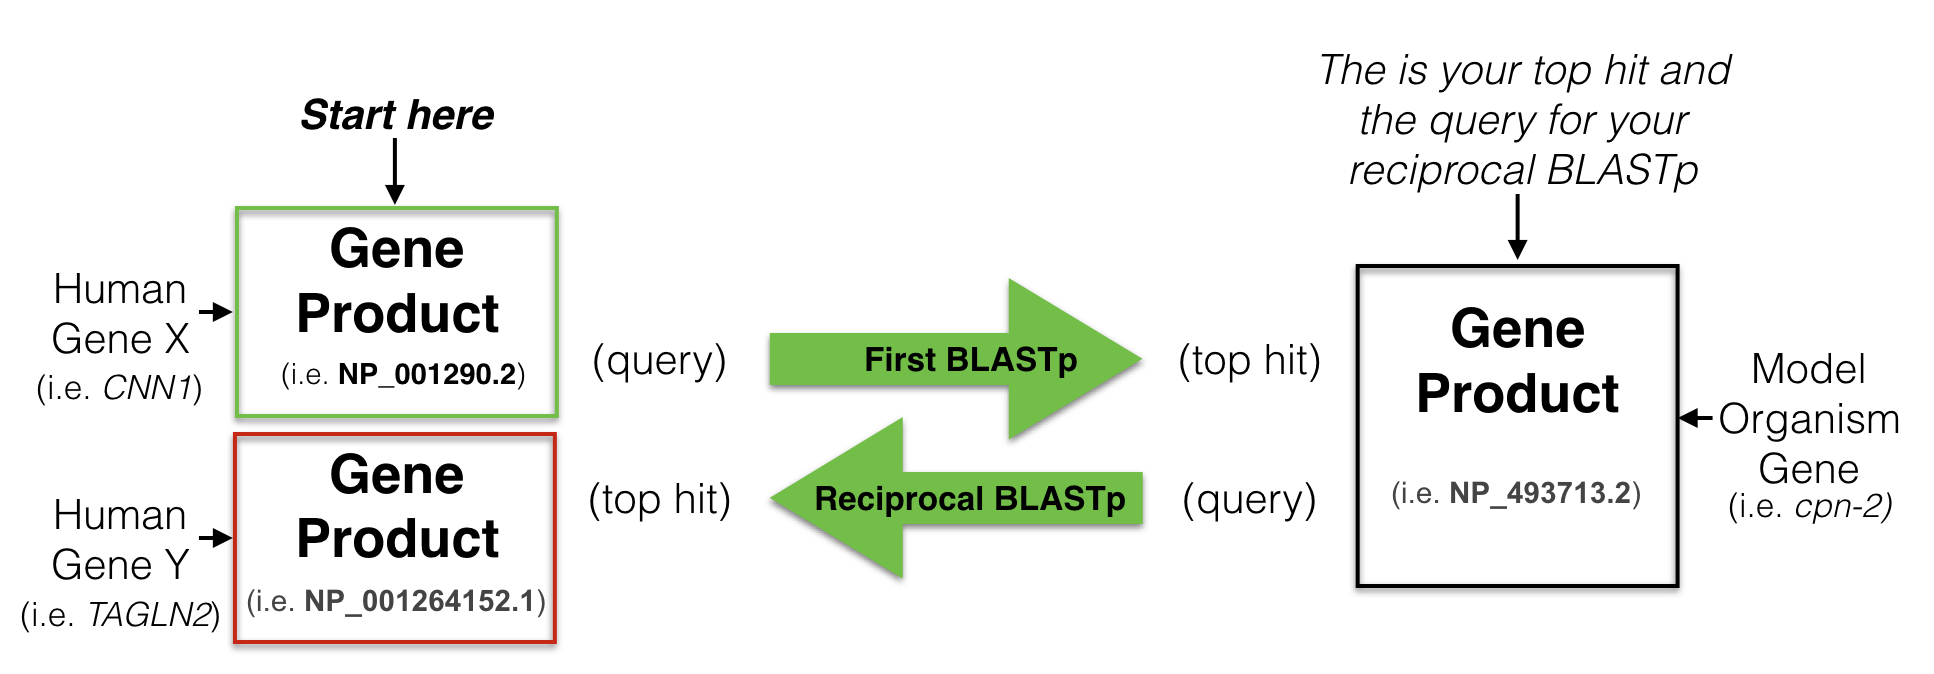
\includegraphics[width=0.75\linewidth]{static/images/RBH2}

}

\caption{A schematic diagram to another possible outcome for a reciptrocal best hit analysis. See text for details.}\label{fig:alternativeRBHoutcome}
\end{figure}

When the the Refseq Protein Accession IDs do not match you need to \emph{confirm} that they are gene products of \emph{different} genes before you claim that they are NOT orthologous. \emph{Recall, a gene can produce multiple protein isoforms! Thus, one gene can have multiple protein Accession number ID codes.} Where can you find this information? One way, go to the protein information page for each protein Refseq ID and search (Control F) for the gene annotation buried at the bottom of the page. (Figure \ref{fig:officialgenename}).

\begin{figure}

{\centering 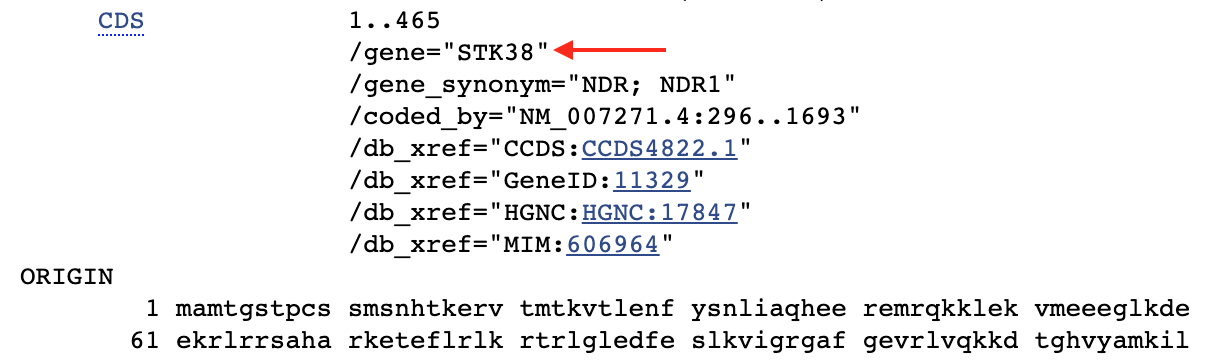
\includegraphics[width=0.75\linewidth]{static/images/GeneName}

}

\caption{This is a screenshot of a small portion of a protein information page for [NP_009202.1](https://www.ncbi.nlm.nih.gov/protein/NP_009202.1). The CDS annotation includes information about the gene. The official gene corresponding to this protein is STK38. This is the gene name used by the UCSC genome browser. Search for it!}\label{fig:officialgenename}
\end{figure}

\textbf{Take home Message:}

When one does an RBH analysis, protein sequences are used to perform each BLASTP (first and reciprocal). \emph{But} a reciprocal best hit successfully identifies a pair of orthologs when it identifies a pair of \textbf{\emph{genes}} that are \emph{eachother's} best hit. The BLASTP is used as a tool to identify those genes.

\hypertarget{test-your-understanding-27}{%
\subsection{\texorpdfstring{\href{https://docs.google.com/forms/d/e/1FAIpQLSdpIxVjTG0lSzcHmQr_21sdnyP5tj6GgEZI0MjvFeflmLqkiQ/viewform?usp=sf_link}{Test Your Understanding}}{Test Your Understanding}}\label{test-your-understanding-27}}

Perform a reciprocal best hit analysis of human ACVR1 using \href{https://www.ncbi.nlm.nih.gov/protein/NP_001334596.1}{NP\_001334596.1} as your query and the Refseq protein database from \emph{Caenorhabditis elegans} as your Subject in the first BLASTP.

\begin{itemize}
\tightlist
\item
  \emph{What is the top hit in C. elegans following your first BLASTP? Provide the Refseq Accession Code.}
\item
  \emph{What is the name of the gene corresponding to the top hit in C. elegans. Find the gene name on the protein information page linked to the refseq accession code.}
\item
  \emph{What is the top hit in H. sapiens following your reciprocal BLASTP? Provide the Refseq Accession Code.}
\item
  \emph{What is the name of the gene corresponding to the top hit found in H. sapiens following your reciprocal BLASTP? Find the gene name on the protein information page linked to the refseq accession code.}
\item
  \emph{Based on the results of your RBH analysis, does C. elegans have a putative ortholog of human ACVR1?}
\end{itemize}

Perform a reciprocal best hit analysis of human PICALM using \href{https://www.ncbi.nlm.nih.gov/protein/NP_009097.2}{NP\_009097.2} as your query and the Refseq protein database from \emph{Caenorhabditis elegans} as your Subject in the first BLASTP.

\begin{itemize}
\tightlist
\item
  \emph{What is the top hit in C. elegans following your first BLASTP? Provide the Refseq Accession Code.}
\item
  \emph{What is the name of the gene corresponding to the top hit in C. elegans. Find the gene name on the protein information page linked to the refseq accession code.}
\item
  \emph{What is the top hit in H. sapiens following your reciprocal BLASTP? Provide the Refseq Accession Code.}
\item
  \emph{What is the name of the gene corresponding to the best hit found in H. sapiens following your reciprocal BLASTP? Find the gene name on the protein information page linked to the refseq accession code.}
\item
  \emph{Based on the results of your RBH analysis, does C. elegans have a putative ortholog of human ACVR1?}
\end{itemize}

\hypertarget{homework-2}{%
\section{\texorpdfstring{\href{https://drive.google.com/file/d/1CWf927mnP3droqocuIpVahigShlSgt6R/view?usp=sharing}{Homework}}{Homework}}\label{homework-2}}

\hypertarget{independent-project}{%
\section{\texorpdfstring{\href{https://drive.google.com/file/d/1uDrvFGWak0VfqcvS_N6fbTqZ_-hIk7Y1/view?usp=sharing}{Independent Project}}{Independent Project}}\label{independent-project}}

Due: TBD

© 2019, Maria Gallegos. All rights reserved.

\end{document}
